\documentclass[12pt,twoside,a4paper,leftblank,vi,openright]{mitthesis}
\usepackage{cmap}
\usepackage[utf8]{inputenc}
\usepackage[T1]{fontenc}
\usepackage{mathtools}
\usepackage{amsmath}
\usepackage{amssymb}
\usepackage[main=english,ngerman,esperanto]{babel}
\usepackage[english=british]{csquotes}
\usepackage{caption}
\usepackage{booktabs}
\usepackage{colortbl}
\usepackage{multirow}
\usepackage{expex}
\usepackage{graphicx}
\usepackage[final,colorlinks]{hyperref}
\usepackage[normalem]{ulem}
\usepackage[backend=biber,style=authoryear-comp,natbib=true]{biblatex}
\addbibresource{content/matter/bibliography.bib}
\AtBeginRefsection{\GenRefcontextData{sorting=ynt}}
\AtEveryCite{\localrefcontext[sorting=ynt]}
\usepackage{stmaryrd}
\SetSymbolFont{stmry}{bold}{U}{stmry}{m}{n}
\usepackage{tikz}
\usepackage{pgfplots}\pgfplotsset{compat=1.17}
\usepackage{qtree}
\usepackage{bbm}
\usepackage{mfirstuc}
\usepackage{stackengine,scalerel}
\usepackage{soul}
\usepackage{ulem}
\usepackage[section,notbib]{tocbibind}
\usepackage{changepage}
\usepackage{svg}
\usepackage{microtype}
\hbadness=99999
\vbadness=99999
\hfuzz=100pt
\clubpenalty10000
\widowpenalty10000
\displaywidowpenalty=10000
\pagestyle{plain}
\setcounter{tocdepth}{4}
\setcounter{secnumdepth}{4}
\addtolength{\skip\footins}{1pc plus 5pt}
\captionsetup[table]{skip=10pt}
\captionsetup{labelfont=bf}
\graphicspath{{content/graphics/}}
\usetikzlibrary{decorations.text,calc,arrows.meta,shapes.geometric}
\newcommand*{\blankpage}{%
\vspace*{\fill}
{\centering THIS PAGE INTENTIONALLY LEFT BLANK\par}
\vspace{\fill}}
\makeatletter
\renewcommand*{\cleardoublepage}{\clearpage\if@twoside \ifodd\c@page\else
\blankpage
\thispagestyle{empty}
\newpage
\if@twocolumn\hbox{}\newpage\fi\fi\fi}
\makeatother
\makeatletter
\g@addto@macro\@floatboxreset\centering
\makeatother
\newcommand{\leadingzero}[1]{\ifnum #1<10 0\the#1\else\the#1\fi}
\newcommand{\todayI}{\the\year-\leadingzero{\month}-\leadingzero{\day}}
\newcommand{\labpage}[1]{\label{page:#1}}
\newcommand{\labpart}[1]{\label{part:#1}}
\newcommand{\labch}[1]{\label{ch:#1}}
\newcommand{\labapp}[1]{\label{app:#1}}
\newcommand{\labsec}[1]{\label{sec:#1}}
\newcommand{\labfig}[1]{\label{fig:#1}}
\newcommand{\labtab}[1]{\label{tab:#1}}
\newcommand{\labdef}[1]{\label{def:#1}}
\newcommand{\labex}[1]{\label{ex:#1}}
\newcommand{\refpage}[1]{\hyperref[page:#1]{Page \ref*{page:#1}}}
\newcommand{\refpart}[1]{\hyperref[part:#1]{Part \ref*{part:#1}}}
\newcommand{\refch}[1]{\hyperref[ch:#1]{Chapter~\ref*{ch:#1}}}
\newcommand{\refapp}[1]{\hyperref[app:#1]{Appendix~\ref*{app:#1}}}
\newcommand{\refsec}[1]{\hyperref[sec:#1]{Section~\ref*{sec:#1}}}
\newcommand{\reffig}[1]{\hyperref[fig:#1]{Figure~\ref*{fig:#1}}}
\newcommand{\reftab}[1]{\hyperref[tab:#1]{Table~\ref*{tab:#1}}}
\newcommand{\refdef}[1]{(\ref*{def:#1})}
\newcommand{\refex}[1]{\hyperref[ex:#1]{(\ref*{ex:#1})}}

\DeclareNameFormat{labelname:poss}{%
  \nameparts{#1}%
  \ifcase\value{uniquename}%
    \usebibmacro{name:family}{\namepartfamily}{\namepartgiven}{\namepartprefix}{\namepartsuffix}%
  \or
    \ifuseprefix
      {\usebibmacro{name:given-family}{\namepartfamily}{\namepartgiveni}{\namepartprefix}{\namepartsuffixi}}
      {\usebibmacro{name:given-family}{\namepartfamily}{\namepartgiveni}{\namepartprefixi}{\namepartsuffixi}}%
  \or
    \usebibmacro{name:given-family}{\namepartfamily}{\namepartgiven}{\namepartprefix}{\namepartsuffix}%
  \fi
  \usebibmacro{name:andothers}%
  \ifnumequal{\value{listcount}}{\value{liststop}}{'s}{}}
\DeclareFieldFormat{shorthand:poss}{%
  \ifnameundef{labelname}{#1's}{#1}}
\DeclareFieldFormat{citetitle:poss}{\mkbibemph{#1}'s}
\DeclareFieldFormat{label:poss}{#1's}
\newrobustcmd*{\citeposalias}{%
  \AtNextCite{%
    \DeclareNameAlias{labelname}{labelname:poss}%
    \DeclareFieldAlias{shorthand}{shorthand:poss}%
    \DeclareFieldAlias{citetitle}{citetitle:poss}%
    \DeclareFieldAlias{label}{label:poss}}}
\newrobustcmd*{\citepos}{%
  \citeposalias%
  \textcite}
\newrobustcmd*{\Citepos}{\bibsentence\citepos}
\newrobustcmd*{\citeposs}{%
  \citeposalias%
  \textcites}
\def\beginsubsub{%
\par
\begingroup
\advance\leftskip by 2em
\def\b##1{\par\leavevmode\llap{\hbox to 2em{##1\hfil}}\ignorespaces}}
\def\endsubsub{\par\endgroup}
\newcommand{\intension}[2][g]{\llbracket\text{#2}\rrbracket^{#1}}
\newcommand{\predicate}[1]{\text{\scshape{#1}}}
\newcommand{\textiff}{1\text{~~iff~~}}
\newcommand{\cf}{\ensuremath{\mathrel{\Box\kern-1.5pt\raise1pt\hbox{$\mathord{\rightarrow}$}}}}
\stackMath
\def\trianglelefteqslant{\ThisStyle{\mathrel{%
  \stackinset{r}{.75pt+.15\LMpt}{t}{.1\LMpt}{\rule{.3pt}{1.1\LMex+.2ex}}{\SavedStyle\leqslant}%
}}}
\newcommand{\lprob}{\triangleleft}
\newcommand{\leqprob}{\trianglelefteqslant}
\newcommand{\speaker}[1]{\textbf{#1:~}}
\newcommand{\context}[1]{\textit{#1}\\}
\newcommand{\contextpex}[1]{\textit{#1}}
\newcommand{\extitle}[1]{\underline{#1}\\}
\newcommand{\pextitle}[1]{\underline{#1}}
\newcommand{\emptyfill}{\hbox{}\hfill}
\pgfmathdeclarefunction{gauss}{2}{%
  \pgfmathparse{1/(#2*sqrt(2*pi))*exp(-((x-#1)^2)/(144*#2^2))}%
}

\def\tmp#1#2#3{%
  \definecolor{Hy#1color}{#2}{#3}%
  \hypersetup{#1color=Hy#1color}}
\tmp{link}{HTML}{800006}
\tmp{cite}{HTML}{2E7E2A}
\tmp{file}{HTML}{131877}
\tmp{url} {HTML}{8A0087}
\tmp{menu}{HTML}{727500}
\tmp{run} {HTML}{137776}
\def\tmp#1#2{%
  \colorlet{Hy#1bordercolor}{Hy#1color#2}%
  \hypersetup{#1bordercolor=Hy#1bordercolor}}
\tmp{link}{!60!white}
\tmp{cite}{!60!white}
\tmp{file}{!60!white}
\tmp{url} {!60!white}
\tmp{menu}{!60!white}
\tmp{run} {!60!white}

\makeatletter
\newcommand{\ChapterOutsidePart}{%
   \def\toclevel@chapter{-1}\def\toclevel@section{0}\def\toclevel@subsection{1}}
\newcommand{\ChapterInsidePart}{%
   \def\toclevel@chapter{0}\def\toclevel@section{1}\def\toclevel@subsection{2}}
\makeatother

\makeatletter
\def\@endpart{\vfil\newpage\if@twoside \if@openright
\mbox{}
\vspace*{\fill}
\begin{center}
{THIS PAGE INTENTIONALLY LEFT BLANK}
\end{center}
\vspace{\fill}
\thispagestyle{empty}
\newpage\fi\fi
\if@tempswa\twocolumn\fi}
\makeatother

\makeatletter
\protected\def\blx@langsetup#1{%
  \blx@lbxinput{#1}
    {\edef\blx@languagename{#1}}
    {}}
\makeatother

\DeclareQuoteStyle{esperanto}{\guillemotleft}{\guillemotright}{\guilsinglleft}{\guilsinglright}

\begin{document}\pagenumbering{roman}

\title{The Semantics and Pragmatics of Counterfactual Sentences at the Discourse Level: Sobel-Sequences and the Licensing of Negative Polarity Items}

\author{David Krassnig}
\department{Department of Linguistics}

\degree{Doctor of Philosophy}

\degreemonth{May}
\degreeyear{2023}
\thesisdate{MAY 22, 2023}


\supervisor{Mar\'ia Isabel Romero Sang\"uesa}{Professor}

\chairman{Someone B. Chairman}{Chairman, Department Committee on Graduate Theses}

\definecolor{konstanz}{RGB}{0,169,224}
\setulcolor{konstanz}
\setul{3pt}{1.5pt}
\begin{titlepage}\doublespacing
\begin{adjustwidth}{-4mm}{-4mm}
\begin{center}
\textbf{\huge The Semantics and Pragmatics of Counterfactual Sentences at the Discourse Level: Sobel-Sequences and the Licensing of Negative Polarity Items}
\end{center}
\end{adjustwidth}

\textbf{\large Doctoral Thesis for Obtaining the Academic Degree\\ Doctor of Philosophy (Dr.~phil.)}

submitted by\\{\large \textit{David Krassnig}}%

at the\\\vspace{-2.5mm}

\includegraphics[scale=0.25]{content/graphics/unikonstanz_signet}


{\large\scshape Faculty of Humanities\\
Department of Linguistics}


Konstanz, 2023
\end{titlepage}
\thispagestyle{empty}
\hbox{}\vfill\begin{flushleft}
\noindent\textbf{{Doctoral Thesis of the University of Konstanz}}

\enlargethispage{3\baselineskip}\noindent\textbf{Day of the oral examination:} 22\textsuperscript{nd} May 2023\\
\textbf{Referee:} Prof. Dr. Maribel Romero\\
\textbf{Referee:} Prof. Dr. Regine Eckardt\\
\textbf{Referee:} Asst. Prof. Dr. María Biezma
\end{flushleft}


\cleardoublepage%
\thispagestyle{empty}
\phantomsection\addcontentsline{toc}{chapter}{\protect Front Matter}%
\hbox{}\vskip 10mm
\begin{flushright}\doublespacing
\textit{\LARGE Life Before Death}\\
\textit{\LARGE Strength Before Weakness}\\
\textit{\LARGE Journey Before Destination}\\\vskip -2mm
\resizebox{81.4mm}{!}{\textbf{from Brandon Sanderson's \textit{The Stormlight Archive}}}
\end{flushright}
\enlargethispage{3\baselineskip}\vfill
\begin{center}\singlespacing
\includesvg[width=33.33mm]{content/graphics/newestvector_hatched.svg}
\end{center}

\cleardoublepage
\section*{Acknowledgements}\addcontentsline{toc}{section}{\protect Acknowledgements}%
First and foremost, I would like to express my deepest gratitude to the best supervisor of all possible worlds, Maribel Romero. If it were not for her, I very likely would not have become a semanticist: Having attended my first seminar on semantics with her as an instructor, I was not only captivated by the rigorous logic of formal semantics but also by her practically endless enthusiasm for her field of study. I could not have wished for a better supervisor, both in a professional and in an interpersonal capacity.

I would also like to express my deepest appreciation to Mar\'ia Biezma, my first second supervisor. She always made sure that I do not consider any given issue in isolation but in the broader context of language, always keeping the bigger picture in mind. She is also largely at fault for me warming up to formal pragmatics, when I originally studied only formal semantics.

I am also very thankful to my second second supervisor, Regine Eckardt. She finished the job that Mar\'ia had started with regards to formal pragmatics. Special thanks to her are due for agreeing to supervise my thesis committee.

I would further like to extend my sincere thanks to my predecessor, Andreas Walker. Having been the only PhD candidate in the field of semantics at the beginning of his studies at the University of Konstanz , he greatly influenced the culture of the emergent circle of fledgling semanticists in Konstanz. The friendly, egalitarian, and ridiculously supportive environment that I experienced in my time as a PhD student there is, in part, a testament to his tremendously caring nature and his dedication to leaving this world a better place.

Along this line of thought, I would also like to express my gratitude to my fellow PhD candidate and long-time office mate, Mark-Matthias Zymla. We had countless conversations on the nature of language and meaning, and even more discussions about the most inane and ridiculous things. He is, I think, partly responsible for me having kept my sanity during the often stressful times leading up to this dissertation.

Naturally, I also give many thanks to all of my other fellow semanticists and pragmaticists at the University of Konstanz. This includes but is not limited to Moritz Meßmer, Felicitas Enders, Erlinde Meertens, Gisela Disselkamp (geb. Grohne), Felix Frühauf, Maryam Mohammadi, Ramona Baumgartner (geb. Wallner), Kajsa Dj\"{a}rv, Arno Goebel, Vasiliki Erotokritou, Yvonne Viesel, Katerina Kalouli, Sven Lauer, Brian Leahy, Eva Csipak, Ryan Bochnak, Todor Koev, and Chen-An Chang.

There are also numerous linguists outside of this university to whom I would like to extend my deepest thanks for meeting with me and/or for providing me with their very insightful comments on my work, including but not limited to Prof.~Dr.~Luka Crni\v{c}, Prof.~Dr.~Kai von Fintel, Prof.~Dr.~Peter Klecha, Prof.~Dr.~Lucas Champollion, and Prof.~Dr.~Irene Heim.

I would also like to thank the research group \enquote{What if? On the Epistemological, Pragmatic, Psychological and Cultural Significance of Counterfactual Thinking} for funding large parts of my research. I would also like to thank each of the research group members for their support, comments, and help over the years. Here, very special thanks go to Prof. Dr. Wolfgang Spohn who masterfully organised and advocated for this research group.

But I must reserve my greatest of thanks to my family: to Stefan, the best big brother who always has my back; to my mother and to my father, Roswitha and Karl-Heinz, who always loved and supported me without condition or reservation; to Blacky, for having been my best friend for nearly two decades, may he rest in peace; to Anna, for being as close to a twin as a cousin can be; to my grandmothers, Oma K\"athe and Oma Resi, for never once making me doubt all the best stereotypes about grandmothers; to my mother-in-law, Mary, for taking me in as if I was her own and, in turn, discrediting all stereotypes about mother-in-laws; to my sisters-in-law, Leyla and Melissa, for being the crazy little sisters I never had; and to my father-in-law, for all he has sacrificed for his family.

Finally, to my wife, Sarah Ceylan Krassnig: You are the great love of my life and \enquote{If I had not met you, I would never have been complete} is the only counterfactual conditional that I would never fathom to be part of a felicitous Sobel sequence.
\cleardoublepage
\section*{Abstract (English)}\addcontentsline{toc}{section}{\protect Abstract (English)}%
In this thesis, I explore the question whether conditionals can be more accurately modelled with a \mbox{(semi-)}dynamic strict \parencite{Fintel2001,Gillies2007} or a variably-strict \parencite{Stalnaker1968,Lewis1973} semantics. To this end, I examine two linguistic phenomena that are associated with conditionals: (weak) negative polarity items and (reverse) Sobel sequences. Negative polarity items are words with a varyingly restrictive distribution that mostly (but not exclusively) occur in negative contexts (e.g., \textit{any} and \textit{ever}). Sobel sequences are conditional sequences that adhere to the pattern of \enquote{If $\phi$, $\chi$; but if $\phi\land\psi$, $\neg\chi$}. 

For negative polarity items, I rule out the traditional account that stipulated that they are licensed by downward monotone environment \parencite{Fauconnier1975a,Fauconnier1975b,Ladusaw1980} due to the contextually changing licensing of negative polarity items in non-monotone environments \parencite{Crnic2011}. This account would have restricted us to a (semi-)dynamic conditional semantics, which is (Strawson) downward monotone by nature, as the variably-strict semantics is non-monotone by nature. I then evaluate an alternative approach to negative polarity item licensing: the operator-based approach that stipulates that negative polarity items are licensed by a covert \textit{even}-like operator that imposes a probability-based scalar presupposition on its associated sentences \parencite[see, amongst others,][]{Crnic2014-dogma,Crnic2014-nm}. I improve the viability of this model by solving an issue that this model had with deriving a difference in question bias between questions containing unfocused weak negative polarity items and questions that contain the expression \textit{even \MakeUppercase{one}} \parencite[see, amongst others,][]{Crnic2014-dogma,Crnic2014-nm,Krassnig2018,Jeong2021,Jeong2022}. I then evaluate the interaction of this licensing model with a variably-strict conditional semantics and with a (semi-)dynamic strict conditional semantics. I show that the latter has a slight explanatory advantage over the former, being able to account for all of the known data, but conclude that this advantage might be mitigated by future research.

(Reverse) Sobel sequences have traditionally been considered another key piece in the debate on how to accurately model conditionals because regularly ordered Sobel sequences are felicitous but reverse Sobel sequences are infelicitous. This status originally spoke in favour of a (semi-)dynamic strict semantics, which was designed to predict reverse Sobel sequences to be infelicitous, because the variably-strict semantics predicts that either sequence type should be felicitous. However, recent developments have shown that some reverse Sobel sequences might be consistently rendered felicitous \parencite{Moss2012}, prompting a return to the variably-strict approach to conditionals with the addition of different selective pragmatic mechanisms that rule out some but not all reverse Sobel sequences \parencite{Moss2012,Klecha2014,Klecha2015,Lewis2018,Krassnig2017,Krassnig2020,Krassnig2022,Ippolito2020}. I survey the current empirical landscape on reverse Sobel sequences and improve upon it by conducting a reverse Sobel sequence felicity experiment. I conclude that the crucial factor for reverse Sobel sequence felicity is contrastive stress in the antecedent of the $\phi$-conditional and isolate a number of highly influential sub-factors for felicity that were partly already proposed in the literature in isolation: namely, (i) counterfactuality, (ii) a lack of a causal link between $\phi$ and $\psi$, and (iii) the use of overt or covert exclusion of $\psi$ as an epistemic possibility (the last of which acts as a felicity rescue operation for contrastively stressed reverse Sobel sequences). I propose a pragmatic model constructed around the effect of contrastive stress and show how this model is able to account for all of the known empirical data on reverse Sobel sequences via the interaction of contrastive stress and the aforementioned factors (where all components can be independently motivated by other phenomena in the literature). Crucially, I show that this proposed supererogatory pragmatic mechanism may be combined with either the variably-strict model or the (semi-)dynamic strict model without a change in the predicted felicity distribution (though the former requires a few additional independently motivated pragmatic mechanisms to do so).

In the end, I conclude that the (semi-)dynamic strict account appears to have a slight explanatory advantage over the variably-strict approach overall, but I also conclude that this advantage can likely be eliminated with further modifications to the variably-strict approach, rendering both approaches equally viable with respect to (reverse) Sobel sequences and negative polarity items.


\cleardoublepage
\section*{Abstract (German)}\addcontentsline{toc}{section}{\protect Abstract (German)}%
\begin{otherlanguage}{ngerman}
In dieser Dissertation untersuche ich die Frage, ob Konditionale eher mit einer \mbox{(semi-)}\linebreak dynamisch strikten \parencite{Fintel2001,Gillies2007} oder einer variabel-strikten Semantik \parencite{Stalnaker1968,Lewis1973} modelliert werden können. Zu diesem Zwecke untersuche ich zwei linguistische Phänomene, die mit Konditionalen assoziiert werden: (schwache) negative Polaritätselemente und (umgekehrte) Sobel-Sequenzen. Negative Polaritätselemente sind Worte mit einer unterschiedlich stark restriktiven Verteilung, die hauptsächlich (aber nicht exklusiv) in negativen Kontexten auftauchen (z.B. \textit{any} und \textit{ever} im Englischen). Sobel-Sequenzen sind Konditionalsequenzen, die dem Muster \glqq Falls $\phi$, $\chi$; aber falls $\phi\land\psi$, $\neg\chi$\grqq\ entsprechen.
    
Für negative Polaritätselemente schließe ich, aufgrund der kontextuell-variablen Lizensierung von negativen Polaritätselementen in nicht-monotonen Umgebungen \parencite{Crnic2011},  die traditionelle Lizensierungstheorie aus, welche davon ausgeht, dass negative Polaritätselemente durch abwärts monotone Umgebung lizensiert werden \parencite{Fauconnier1975a,Fauconnier1975b,Ladusaw1980}. Da die variabel-strikte semantik nicht-\linebreak monotoner Natur ist, hätte uns diese Theorie auf eine (semi-)dynamische strikte Semantik, welche (Strawson) abwärts monotoner Natur ist, eingeschränkt. Ich evaluiere dann einen alternativen Ansatz zur Lizensierung von negativen Polaritätselementen: der Operator-basierende Ansatz, welcher davon ausgeht, dass negative Polaritätselemente durch einen verdeckten \textit{even}-ähnlichen Operator lizensiert werden, der den verbundenen Sätzen, in denen er vorkommt, eine auf Wahrscheinlichkeiten basierende Skalarpräsupposition auferlegt \parencite[siehe, unter anderem][]{Crnic2014-dogma,Crnic2014-nm}. Ich verbessere die Viabilität dieses Modells dadurch, dass ich ein Problem löse, das dieses Modell hatte: die Herleitung des Unterschiedes in negativer Voreingenommenheit zwischen Fragen, die ein unfokusiertes schwaches negatives Polaritätselement beinhalten, und Fragen, die den Ausdruck \textit{even ONE}\footnote{Das nächstgelegene deutsche Äquivalent zu \textit{even ONE} wäre \textit{auch nur EIN}.} beinhalten \parencite[vgl.][]{Crnic2014-dogma,Crnic2014-nm,Krassnig2018,Jeong2021,Jeong2022}. Dann evaluiere ich die Interaktion dieses Lizensierungsmodells mit einer variabel-strikten Semantik und einer (semi-)dynamisch strikten Semantik. Ich zeige, dass die Letztere einen schwachen explanativen Vorteil gegenüber der Ersteren hat, dass die Letztere alle bekannten Fakten erklären kann, aber auch dass dieser Vorteil eventuell durch zukünftige Forschung abgeschwächt werden könnte.
    
(Umgekehrte) Sobel-Sequenzen werden traditionell als weiterer Schlüsselfaktor in der Debatte darüber, wie Konditionale am besten modelliert werden können, betrachtet, da regulär geordnete Sobel-Sequenzen als gelungen und umgekehrte Sobel-Sequenzen als mißlungen gelten. Da die variabel-strikte Semantik vorhersagt, dass beide Sequenztypen gelungen sein sollten, sprach dieser Status ursprünglich für eine \mbox{(semi-)}dynamische strikte Semantik, die dafür entworfen wurde, umgekehrte Sobel-\linebreak Sequenzen als mißlungen vorherzusagen. Neuere Entwicklungen haben jedoch aufgezeigt, dass einige umgekehrte Sobel-Sequenzen konsistent als gelungen eingestuft werden können \parencite[vgl.][]{Moss2012}. Dies führte zu einer Rückkehr zum variabel-strikten Ansatz zu Konditionalen mit der Hinzufügung verschiedener selektiver pragmatischer Mechanismen, die einige aber nicht alle umgekehrte Sobel-Sequenzen ausschließen \parencite[vgl.][]{Moss2012,Klecha2014,Klecha2015,Lewis2018,Krassnig2017,Krassnig2020,Krassnig2022,Ippolito2020}. Ich untersuche die Genauigkeit der aktuellen empirischen Landschaft von umgekehrten Sobel-Sequenzen und verbessere diese durch die Durchführung eines  Experiments, welche umgekehrte Sobel-Sequenzen auf ihre Gelungenheit untersucht. Dann schlussfolgere ich, dass der entscheidende Faktor für die Gelungenheit von umgekehrten Sobel-Sequenzen der kontrastive Stress im Antezedenten der $\phi$-Konditionale ist und isoliere eine Anzahl von einflussreichen Unterfaktoren für Gelungenheit, die teilweise bereits in der Literatur isoliert vorgeschlagen wurden: nämlich (i)~Kontrafaktualität, (ii)~das Fehlen eines kausalen Zusammenhangs zwischen $\phi$ und $\psi$ und (iii)~die Verwendung eines offenen oder verdeckten Ausschlusses von $\psi$ als epistemische Möglichkeit (Letzteres fungiert als Gelungenheit-Rettungsoperation für kontrastiv betonte umgekehrte Sobel-Sequenzen). Ich schlage ein pragmatisches Modell vor, das um den Effekt des kontrastiven Stresses herum aufgebaut ist, und zeige auf, wie dieses Modell durch die Interaktion zwischen dem kontrastiven Stress und den vorher genannten Faktoren alle bekannten empirischen Daten zu umgekehrten Sobel-Sequenzen korrekt vorhersagen kann (wobei alle Komponenten durch andere Phänomene in der Literatur unabhängig motiviert werden können). Schlussendlich zeige ich, dass dieser vorgeschlagene pragmatische Mechanismus entweder mit dem variabel-strikten Modell oder mit dem (semi-)dynamischen strikten Modell kombiniert werden kann, ohne dass sich die vorhergesagte Gelungenheitsdistribution verändert (wobei letztere Semantik einige zusätzliche unabhängig motivierte pragmatische Mechanismen erfordert).
    
Am Ende schlussfolgere ich, dass das (semi-)dynamische strikte Modell insgesamt einen leichten explanativen Vorteil gegenüber dem variabel-strikten Ansatz hat. Ich schlussfolgere aber auch, dass dieser Vorteil wahrscheinlich durch weitere Modifikationen des variabel-strikten Ansatzes eliminiert werden kann, wodurch beide Ansätze in Bezug auf (umgekehrte) Sobel-Sequenzen und negative Polartitäts-Elemente gleichermaßen tragfähig werden würden.
\end{otherlanguage}

\cleardoublepage
\section*{Abstract (Esperanto)}\addcontentsline{toc}{section}{\protect Abstract (Esperanto)}%
\begin{otherlanguage}{esperanto}\setquotestyle{esperanto}
En ĉi tiu disertaĵo, mi esploras la demandon ĉu oni povas modeli kondiĉfrazojn pli precize per (duon-)dinamika strikta semantiko \parencite{Fintel2001,Gillies2007} aŭ variabla-strikta semantiko \parencite{Stalnaker1968,Lewis1973}. Por tio, mi ekzamenas du lingvajn fenomenojn kiuj estas asociitaj kun kondiĉfrazoj: (malfortajn) negativajn polusaĵojn kaj (inversajn) Sobel-sekvencojn. Negativaj polusaĵoj estas vortoj kun varie restriktiva distribuo kiuj plejparte (sed ne ekskluzive) aperas en negativaj kuntekstoj (ekz. \textit{any} kaj \textit{ever} en la angla). Sobel-sekvencoj estas kondiĉfrazaj sekvencoj kiuj obeas al la ŝablono de \enquote{Se $\phi$, $\chi$; sed se $\phi\land\psi$, $\neg\chi$}.

Por negativaj polusaĵoj, mi forĵetas la tradician klarigon, kiu asertis ke negativaj polusaĵoj permesiĝas per malsuprene monotonaj medioj \parencite{Fauconnier1975a,Fauconnier1975b,Ladusaw1980}, pro la kuntekste ŝanĝiĝanta permesigeco de negativaj polusaĵoj en ne-monotonaj medioj \parencite{Crnic2011}. Tiu klarigo restriktus nin al (duon-)dinamika kondiĉfraza semantikoj, kiu estas (Strawson-e) malsupre monotona medie, ĉar la variabla-strikta semantiko estas ne-monotona medie. Mi tiam taksas alternativan aliron al la permesigeco de negativaj polusaĵoj: la operatora aliro kiu asertas ke negativaj polusaĵoj permesiĝas per kaŝa \textit{eĉ}-simila operatoro kiu aldonas probablan skalisan antaŭsupozon al siaj asociitaj frazoj \parencite[vidu, inter aliajn,][]{Crnic2014-dogma,Crnic2014-nm}. Mi plibonigas la vivipoveco de ĉi tiu modelo per solvado problemon kiun ĉi tiu modelo havis pri derivado la malsamon de demando-inkliniĝo inter demandoj kiuj enhavas ne-fokusigatan malfortan negativan polusaĵon kaj demandoj kiuj enhavas la esprimon \textit{eĉ unu} \parencite[vidu, inter aliajn,][]{Crnic2014-dogma,Crnic2014-nm,Krassnig2018,Jeong2021,Jeong2022}. Poste, mi evalvas la interagon de ĉi tiu permesiga modelo kun variabla-strikta kondiĉfraza semantiko kaj kun (duon-)dinamika strikta kondiĉfraza semantiko. Mi montras ke la lasta havas iomajn klarigajn avantaĝojn kontraŭ la unua, ke ĝi povas klarigi ĉiujn konatajn datumojn, sed konkludas ke ĉi tiu avantaĝo povus esti malgrandigita per estonta esplorado.
    
(Inversaj) Sobel-sekvencoj estas tradicie konsideritaj aliaj ĉefaj punktoj en la diskuto pri la preciza modeligo de kondiĉfrazoj, ĉar regule ordigitaj Sobel-sekvencoj estas feliĉumaj, sed inversaj Sobel-sekvencoj estas malfeliĉumaj. Tiu statuso unue favoris (duon-)dinamikan striktan semantikon, kiu estis kreita por antaŭdiri ke inversaj Sobel-sekvencoj estu malfeliĉumaj, ĉar la variabla-strikta semantiko antaŭdiras ke ambaŭ sekvenctipoj estu feliĉumaj. Tamen, lastatempaj evoluoj montris, ke kelkaj inversaj Sobel-sekvencoj povas esti konstante feliĉumaj \parencite{Moss2012}, instigante revenon al la variabla-strikta aliro al kondiĉfrazoj kun aldonaj elektivaj pragmatikaj mekanismoj kiuj elĵetas iujn sed ne ĉiujn inversajn Sobel-sekvencojn \parencite{Moss2012,Klecha2014,Klecha2015,Lewis2018,Krassnig2017,Krassnig2020,Krassnig2022,Ippolito2020}. Mi esploras la nunan empirian pejzaĝon pri inversaj Sobel-sekvencoj kaj plibonigas ĝin per realigo de esperimento pri feliĉumeco de inversaj Sobel-sekvencoj. Mi konkludas, ke la decida faktoro por la aprobo de inversaj Sobel-sekvencoj estas kontrasta streso en la antaŭaĵo de la $\phi$-kondiĉfrazo kaj apartigas kelkajn tre influajn subfaktorojn por aprobo, kiuj estis parte jam proponitaj en la literaturo izole: nome, (i) kontrafaktualeco, (ii) manko de kaŭza ligilo inter $\phi$ kaj $\psi$, kaj (iii) la uzo de malkaŝa aŭ kaŝa ekskludo de $\psi$ kiel epistema ebleco (la lasta el kiuj agas kiel feliĉumeco-savilo por kontraste streseblaj inversaj Sobel-sekvencoj). Mi proponas pragmatikan modelon kiu estas konstruita ĉirkaŭ la efiko de kontrasta streso kaj mi montras kiel ĉi tiu modelo kapablas klarigi ĉiujn konatajn empiriajn datumojn pri inversaj Sobel-sekvencoj per la interago de kontrasta streso kaj la antaŭdiraj faktoroj (kie ĉiuj komponantoj povas esti sendepende motivitaj per aliaj fenomenoj en la literaturo). Grave, mi montras ke ĉi tiu proponita aldona pragmatika mekanismo povas esti kombinita aŭ kun la variabla-strikta modelo aŭ kun la (duon-)dinamika strikta modelo sen ŝanĝo en la antaŭdirita feliĉumeco-distribuo (kvankam la unua postulas kelkajn aldonajn sendepende motivitajn pragmatikajn mekanismojn por plenumi tion).
    
Fine, mi konkludas ke la (duon-)dinamika strikta klarigo ŝajnas havi iometan klarigan avantaĝon kontraŭ la variabla-strikta aliro en la tutaĵo, sed mi ankaŭ konkludas ke ĉi tiu avantaĝo verŝajne povas esti eliminata per pluaj modifoj al la variabla-strikta aliro, farante ambaŭ aliroj egale taŭgaj rilate al (inversaj) Sobel-sekvencoj kaj negativaj polusaĵoj.
\end{otherlanguage}

\cleardoublepage

\pagestyle{plain}
\renewcommand{\contentsname}{Table of Contents}
\tableofcontents
\newpage
\listoffigures
\newpage
\listoftables
\cleardoublepage
\pagenumbering{arabic}
\setcounter{page}{1}
\chapter{Introduction}\labch{intro}
In the field of formal semantics, pinning down the exact nature of the meaning of conditionals has been a long-standing and controversial topic. Our earliest sources on the meaning of conditionals date back to ancient Greece, where Philo the Dialectician, in a debate with his teacher Diodorus Cronus, argued that a conditional is true exactly when it is not the case that the antecedent is true and the consequent is false, as reported by Sextus Empiricus in the second century of the Common Era \parencite{Kneale1962}. This definition gave rise to the analysis of conditionals in \textcite{Frege1879} and \citepos{Whitehead1910} two-valued propositional framework that modern philosophisers refer to as the \enquote{material conditional}, as defined in \refdef{material}.
\ex\phantomsection
$\intension[w,g]{If $\phi$, $\psi$}=\textiff\phi\supset\psi$\\
\phantom{$\intension[w,g]{If $\phi$, $\psi$}=~$}$\textiff\phi\rightarrow\psi$\\
\phantom{$\intension[w,g]{If $\phi$, $\psi$}=~$}$\textiff\neg\phi\lor\psi$\\
\phantom{$\intension[w,g]{If $\phi$, $\psi$}=~$}$\textiff\phi\land\neg\psi$\labdef{material}
\xe
But, as already noted by \textcite{Frege1879} himself, this definition is woefully inadequate when trying to define the meaning of natural language conditionals, as it leads to a number of highly unintuitive properties that are collectively known as the paradoxes of material implication. One of the gravest of these shortcomings is typically considered to be that this model predicts all conditionals to be true so long as their antecedents are false, irrespective of their actual propositional content \parencite{Lewis1912}.

\section{Strict Semantics}
To rectify this issue, providing a first step towards an intensional treatment of conditionals, \textcite[p.~33]{Peirce1896} and \textcite{Lewis1912,Lewis1914,Lewis1918} proposed an analysis of conditionals where the material conditional must not only be true but necessarily true; i.e., the material implication must be true in all (accessible) possible worlds. This approach is referred to as the strict approach to conditional semantics. Using \citepos{Kripke1963} modal logic semantics, \citepos{Lewis1912,Lewis1914,Lewis1918} definition may be expressed as shown in \refex{strict-intro}.
\ex\phantomsection\label{ex:strict-intro}
$\intension[w,g]{If $\phi$, $\psi$.}=\textiff\square(\phi\supset\psi)$
\xe
This definition successfuly avoids the aforementioned paradox of material implication: Even if the antecedent is false in the actual world, we would still have to evaluate whether the material implication is also true in all possible worlds, including worlds where the antecedent is true.

However, whilst being a definite improvement over the material conditional, this traditional strict conditional semantics still carries a number of issues that preclude it from being considered a real candidate for an accurate semantics of natural language conditionals. One of these issues, for example, relates to the fact that \citepos{Lewis1912,Lewis1914,Lewis1918} semantics would predict that conditionals are transitive by nature (i.e., when \enquote{If $\phi$, $\psi$} and \enquote{If $\psi$, $\chi$} are true, then we would expect \enquote{If $\phi$, $\chi$} to be true as well). Natural language conditionals are not, however, universally transitive by nature, as demonstrated by \refex{transitive}.
\ex\phantomsection
If Brown wins the election, Smith will retire to private life. If Smith dies before the election, Brown will win it. \#Therefore, if Smith dies before the election, then he will retire to private life.\hfill\parencite[p.~166]{Adams1965}\labex{transitive}
\xe
Another issue is that of monotonicity. \textcite{Lewis1912,Lewis1914,Lewis1918} would predict that all conditional antecedents are purely downward monotone with regards to all possible worlds. This has two consequences of note: one positive and one negative. 

The positive consequence of note would be that so-called weak negative polarity items would be licensed in the antecedent of conditionals according to their classical environment-/monotonicity-based licensing theory. Weak negative polarity items, such as \textit{any} or \textit{ever}, are words which are restricted in their distribution to certain contexts (most of which are perceived to be negative by nature). Their classical licensing theory posits that they may only ever occur in downward monotone environments \parencite{Ladusaw1980,Fauconnier1975a,Fauconnier1975b}. 
\ex\phantomsection\label{def:dm-intro}%
\extitle{Downward Monotonicity}%
$f\in D_{\langle\sigma,\tau\rangle}$ is downward monotone iff for all $x,y\in D_\sigma$ s.t. $x\subseteq y$: $f(y)\Rightarrow f(x)$.%

\xe
However, empirical data shows that negative polarity items also occur in the antecedent of conditionals:
\ex\phantomsection
If John had read any book, he would've passed the test.\labex{npi-conditional-good-any-intro}
\xe
Since the strict approach to conditionals would render the antecedent of conditionals downward monotone by nature, this model would correctly predict that negative polarity items are licensed in this environment.

The negative consequence of this presumed downward monotonicity, on the other hand, would be as follows: If we have a conditional that was evaluated to be true, any and all conditionals whose antecedents are mere specifications of the original antecedent must necessarily also be true with respect to the original consequent. However, as noted by \textcite[p.~10]{Lewis1973}, this is clearly not the case for all conditionals. In fact, \textcite{Lewis1973} noted that any conditional \enquote{If $\phi$, $\chi$} may have its antecedent further specified by some proposition $\psi$ such that it leads to the negation of the consequent, yielding a conditional along the lines of \enquote{If $\phi\land\psi$, $\neg\chi$}. In addition, the latter may follow the former in a sequence of conditionals without any feeling of contradiction of infelicity. This is shown in \refex{SS-nuclear-intro}.
\ex\phantomsection\labex{SS-nuclear-intro}If the USA threw its weapons into the sea tomorrow, there would be war;\linebreak but if the USA and the other nuclear powers all threw their weapons into the sea tomorrow, there would be peace.\hfill\parencite[p.~10]{Lewis1973}
\xe
Because the first verifiable mention of such conditional sequences in modern science was done by \textcite{Sobel1970}, such sentences are referred to as \textit{Sobel sequences}.
\ex\phantomsection\labdef{SS-intro}\extitle{Sobel Sequence}A Sobel sequence is any sequence of conditionals that adheres to the pattern of \enquote{If $\phi$, $\chi$; [but] if $(\phi\land\psi)$, $\neg\chi$}, where $\phi\neq\psi$.%
\xe
Since the strict conditional semantics assumes that conditional antecedents are downward monotone by nature, we would erroneously predict all Sobel sequences to be contradictory and, therefore, to be infelicitous. This was one of the main motivations behind the development of the so-called variably-strict approach to conditional semantics \parencite{Stalnaker1968,Lewis1973}.


\section{Variably-Strict Semantics}
\textcite{Stalnaker1968} and \textcite{Lewis1973} introduced the notion that at least subjunctive conditionals (e.g., counterfactuals) do not simply quantify over all accessible worlds but merely over a subset of these worlds. More specifically, they quantify only over those possible worlds that fulfil the requirements of the antecedent and that can be considered the least different to the world that the conditional was uttered in (referred to as the evaluation world, which typically though not necessarily coincides with the actual world $w_0$). To achieve this, researchers have introduced the concepts of world similarity as well as world closeness. These terms were often used nigh interchangeably until relatively recently. To differentiate, world closeness refers to ranking each possible world in relation to a specific evaluation world according to some metric, and this metric is typically equal to world similarity (though not necessarily). World similarity, in turn, measures how similar any given possible world should be considered to the evaluation world, and was nigh-simultaneously developed by \textcite{Stalnaker1968}, \textcite{Stalnaker1970}, \textcite{Sprigge1970}, \textcite{Lewis1973}, and \textcite{Nute1975}, but first formulated as a notion by \textcite[p.~107]{Todd1964}:
\begin{displayquote}
When we allow for the possibility of the antecedent’s being true in the case of a counterfactual, we are hypothetically substituting a different world for the actual one. It has to be supposed that this hypothetical world is as much like the actual one as possible so that we will have grounds for saying that the consequent would be realised in such a world.
\end{displayquote}
To this end, \textcite{Lewis1973} counts any additional deviation from the evaluation world as a singular decrease in world similarity.\footnote{This view on similarity leads to a number of problems down the line. A more sensible approach concerning how world similarity is to be measured is introduced in \refsec{css-bennett-explanation} and reflects the work of \textcite{Bennett2003} and \textcite{Arregui2009}.} This similarity ordering is traditionally visually represented by concentric layers, where each layer further out represents an additional decrease in similarity to the evaluation world, which is found at the very centre, as seen in \reffig{similarity-ordering-intro}.
\begin{figure}[!htb]
\begin{tikzpicture}
	\coordinate (O) at (0,0);

	\draw[fill=white] (O) circle (2.05);
	\draw[fill=white] (O) circle (1.475);
	\draw[fill=white] (O) circle (0.9);
	\draw[fill=white] (O) circle (0.325)node {w$_0$};

	\node at (0,0.6) {w$_1$};
	\node at (0.5,-0.4) {w$_2$};
	\node at (-0.5,-0.4) {w$_3$};
	
	\node at (-0.85,0.825) {w$_4$};
	\node at (0.85,0.825) {w$_5$};
	\node at (0,-1.15) {w$_6$};
	
	\node at (-0.85,-1.6) {w$_7$};
	\node at (0.85,-1.6) {w$_8$};
	\node at (0,1.75) {w$_9$};
	
	\node at (0,-2.6) {Similarity Ordering};
\end{tikzpicture}
\caption{Similarity ordering with respect to the evaluation world $w_0$, where the worlds $w_{1\leqslant n\leqslant3}$ are equally similar to $w_0$, but more similar to $w_0$ than $w_{4\leqslant n\leqslant9}$, and where $w_{4\leqslant n\leqslant6}$ are still more similar to $w_0$ than $w_{7\leqslant n\leqslant9}$.}
\labfig{similarity-ordering-intro}
\end{figure}

\noindent We therefore define the variably-strict analysis's conditional semantics as in \refdef{variablystrict-intro}:
\ex\phantomsection\labdef{variablystrict-intro}For all contexts $c$, \enquote{If $\phi$, $\psi$} is true at $w$ in $c$ iff all the closest $\phi$-worlds to $w$ are $\psi$-worlds, where closeness is determined by similarity.%
\xe
Alternatively, the same underlying mechanism can be expressed in a more formalised fashion as shown in \refdef{variablystrictformal-intro}, where the accessibility function $f_\leqslant(p,w)$ returns the set of the $p$-worlds that are closest to the evaluation world $w$.\enlargethispage*{1.5\baselineskip}
\ex\phantomsection\labdef{variablystrictformal-intro}$\intension{If $\phi$, $\psi$}=[\lambda w_s.\forall v:v\in f_\leqslant([\lambda w'_s.\phi(w')],w)[\psi(v)]]$\xe\newpage
\noindent This effectively renders conditionals non-monotonic in their domain of quantification. 
\ex\phantomsection\label{def:nm-intro}%
\extitle{Non-Monotonicity}%
$f\in D_{\langle\sigma,\tau\rangle}$ is non-monotone iff for all $x,y\in D_\sigma$ s.t. $x\subseteq y$:\\$f(y)\not\Rightarrow f(x)$ and $f(x)\not\Rightarrow f(y)$.%

\xe
This has, again, one negative and one positive consequence of note.

For the licensing of negative polarity items in the antecedent of conditionals, the presumed non-monotone nature of conditional antecedents would entail that no weak negative polarity items should be licensed in this environment according to \textcite{Fauconnier1975a,Fauconnier1975b} and \citepos{Ladusaw1980} licensing theory. This is an obviously wrong prediction, given the empirical data shown in \refex{npi-conditional-good-any-intro}.

For Sobel sequences, on the other hand, the result would be a bit more positive. Given the non-monotone nature of antecedents, the $\phi$-conditional no longer considers the worlds of the $\phi\land\psi$-conditional for its own evaluation. Instead, the two conditionals quantify over two completely separate sets of worlds, as illustrated in \reffig{stalnakerlewis-SS-intro}.
\begin{figure}[!htb]
    \begin{tikzpicture}
	\coordinate (O) at (0,0);
    \node at (-2,2) {\textbf{Step 1}};
	\draw[fill=white] (O) circle (2.05);
	\draw[fill=white] (O) circle (1.475);
	\draw[fill=gray!33] (O) circle (0.9);
	\draw[fill=white] (O) circle (0.325)node {w\textsubscript{0}};

	\node at (0,0.6) {\textbf{w\textsubscript{1}}};
	\node at (0.5,-0.4) {\textbf{w\textsubscript{2}}};
	\node at (-0.5,-0.4) {\textbf{w\textsubscript{3}}};
	
	\node at (-0.85,0.825) {w\textsubscript{4}};
	\node at (0.85,0.825) {w\textsubscript{5}};
	\node at (0,-1.15) {w\textsubscript{6}};
	
	\node at (-0.85,-1.6) {w\textsubscript{7}};
	\node at (0.85,-1.6) {w\textsubscript{8}};
	\node at (0,1.75) {w\textsubscript{9}};
	
	\node at (0,-2.6) {If $\phi$, $\chi$};
	
	
	\begin{scope}[xshift=5.5cm]
		\coordinate (O) at (0,0);
        \node at (-2,2) {\textbf{Step 2}};
    \draw[fill=white] (O) circle (2.05);
	\draw[fill=gray!33] (O) circle (1.475);
	\draw[fill=white] (O) circle (0.9);
	\draw[fill=white] (O) circle (0.325)node {w\textsubscript{0}};

	\node at (0,0.6) {w\textsubscript{1}};
	\node at (0.5,-0.4) {w\textsubscript{2}};
	\node at (-0.5,-0.4) {w\textsubscript{3}};
	
	\node at (-0.85,0.825) {\textbf{w\textsubscript{4}}};
	\node at (0.85,0.825) {\textbf{w\textsubscript{5}}};
	\node at (0,-1.15) {\textbf{w\textsubscript{6}}};
	
	\node at (-0.85,-1.6) {w\textsubscript{7}};
	\node at (0.85,-1.6) {w\textsubscript{8}};
	\node at (0,1.75) {w\textsubscript{9}};
	
	\node at (0,-2.6) {If $(\phi\land\psi)$, $\neg\chi$};
	\end{scope}
\end{tikzpicture}
\caption{Domains of quantification for Sobel sequences according to \textcite{Stalnaker1968} and \citepos{Lewis1973} variably-strict conditional analyses. For all $w_n$-worlds: If $n\geqslant1$, then $\phi=1$ is true for $w_n$, and if $n\geqslant 4$, then $\psi=1$ holds true for $w_n$. If $n\geqslant 7$, then some proposition $\omega=1$ such that $\omega\neq\phi$, $\omega\neq\psi$, and $\phi,\psi$ do not precede $\omega$ on some causal chain of events.}
\labfig{stalnakerlewis-SS-intro}
\end{figure}

\noindent Therefore, no conflicting statement is made, rendering Sobel sequences felicitous.

Crucially, the order of the conditionals should be of no further relevance because the set of the closest $\phi$-worlds and the set of the closest $\phi\land\psi$-worlds are disjoint. This does not, however, appear to not be the case: Reverse Sobel sequences---defined in \refdef{rSS-intro}---have traditionally been observed to be infelicitous, even though they, as the name would imply, consist of the same conditionals as a Sobel sequence, merely in reverse order. The infelicity of such sequences is typically demonstrated with the counterpart to \refex{SS-nuclear-intro}, as seen in \refex{rSS-nuclear-intro}, that was originally provided by \textcite{Heim1994}.
\ex\phantomsection\labdef{rSS-intro}\extitle{Reverse Sobel Sequence}A reverse Sobel sequence is any sequence of conditionals that adheres to the pattern of \enquote{If $(\phi\land\psi)$, $\neg\chi$; [but] if $\phi$, $\chi$}, where $\phi\neq\psi$.%
\xe
\ex\phantomsection\labex{rSS-nuclear-intro}If the USA and the other nuclear powers all threw their weapons into the sea tomorrow, there would be peace;\\\ljudge\# but if the USA threw its weapons into the sea tomorrow, there would be war.\\\emptyfill\parencite{Heim1994}
\xe

The hereto illustrated variably-strict conditional analysis fails to predict the infelicity or perceived inconsistency of the reverse Sobel sequence, as the domains of quantification remain entirely disjoint, as seen in \reffig{stalnakerlewis-rSS-intro}:
\begin{figure}[!htb]
\begin{tikzpicture}
	\coordinate (O) at (0,0);
    \node at (-2,2) {\textbf{Step 1}};
	\draw[fill=white] (O) circle (2.05);
	\draw[fill=gray!33] (O) circle (1.475);
	\draw[fill=white] (O) circle (0.9);
	\draw[fill=white] (O) circle (0.325)node {w\textsubscript{0}};

	\node at (0,0.6) {w\textsubscript{1}};
	\node at (0.5,-0.4) {w\textsubscript{2}};
	\node at (-0.5,-0.4) {w\textsubscript{3}};
	
	\node at (-0.85,0.825) {\textbf{w\textsubscript{4}}};
	\node at (0.85,0.825) {\textbf{w\textsubscript{5}}};
	\node at (0,-1.15) {\textbf{w\textsubscript{6}}};
	
	\node at (-0.85,-1.6) {w\textsubscript{7}};
	\node at (0.85,-1.6) {w\textsubscript{8}};
	\node at (0,1.75) {w\textsubscript{9}};
	
	\node at (0,-2.6) {If $(\phi\land\psi)$, $\neg\chi$};
	
	
	\begin{scope}[xshift=5.5cm]
		\coordinate (O) at (0,0);
        \node at (-2,2) {\textbf{Step 2}};
    \draw[fill=white] (O) circle (2.05);
	\draw[fill=white] (O) circle (1.475);
	\draw[fill=gray!33] (O) circle (0.9);
	\draw[fill=white] (O) circle (0.325)node {w\textsubscript{0}};

	\node at (0,0.6) {\textbf{w\textsubscript{1}}};
	\node at (0.5,-0.4) {\textbf{w\textsubscript{2}}};
	\node at (-0.5,-0.4) {\textbf{w\textsubscript{3}}};
	
	\node at (-0.85,0.825) {w\textsubscript{4}};
	\node at (0.85,0.825) {w\textsubscript{5}};
	\node at (0,-1.15) {w\textsubscript{6}};
	
	\node at (-0.85,-1.6) {w\textsubscript{7}};
	\node at (0.85,-1.6) {w\textsubscript{8}};
	\node at (0,1.75) {w\textsubscript{9}};
	
	\node at (0,-2.6) {If $\phi$, $\chi$};
	\end{scope}
\end{tikzpicture}%
\caption{Quantificational domains for reverse Sobel sequences according to \textcite{Stalnaker1968} and \citepos{Lewis1973} variably-strict conditional analyses. For all worlds $w_n$: If $n\geqslant1$, then $\phi=1$ is true for $w_n$, and if $n\geqslant 4$, then $\psi=1$ holds true for $w_n$. If $n\geqslant 7$, then some proposition $\omega=1$ such that $\omega\neq\phi$, $\omega\neq\psi$, and $\phi,\psi$ do not precede $\omega$ on some causal chain of events.}\labfig{stalnakerlewis-rSS-intro}
\end{figure}

\noindent Since the sequence's two relevant domains of quantification are entirely disjoint, it makes---from a semantic point of view---no difference in which order a claim about the respective worlds is made. As such, the variably-strict semantics would falsely predict all reverse Sobel sequences to be felicitous.\vfill
\section{(Semi-)Dynamic Strict Semantics}
The infelicity of reverse Sobel sequences led to a renewed interest in the strict conditional analysis, as that approach correctly predicted the infelicity of reverse Sobel sequences. To account for regularly ordered Sobel sequences, however, the original model requires additional constraints on the domain of quantification, such that Sobel sequences do not yield a contradiction---without affecting the fact that reverse Sobel sequences do. This led to the inception of the (semi-)dynamic strict conditional line of thought, as originally put forth by \textcite{Fintel2001} and \textcite{Gillies2007}. 

\textcite{Fintel2001} proposes that counterfactual conditionals are analysed as strict conditionals that apply to a contextually determined domain of quantification. Counterfactual conditionals also carry a presupposition of entertainability, which means that their antecedents must be possible with respect to the aforementioned contextually defined domain of quantification. If this presupposition is violated---that is, the contextually determined domain of quantification does not contain any antecedent world---then the contextual domain of quantification is expanded to include all possible worlds up to and including the closest possible antecedent worlds. For this reason, \textcite{Fintel2001} also refers to the contextually-expanding domain of quantification as a modal horizon. This operation is formally executed through the accessibility relation $f_\sigma$ as specified by the context $\sigma$ (which initially comprises only the evaluation world itself). If the context lacks any valid antecedent worlds, the respective counterfactual modifies $\sigma$ to include all worlds up to and including the closest antecedent worlds. The modified context is then maintained for any subsequent counterfactual conditionals, with the process of modifying $\sigma$ being repeated as necessary (i.e., whenever no valid antecedent world already exists in the modal horizon).\linebreak\newpage\noindent This entire process in formally defined in its entirety in \refdef{fintel-intro}.
\pex\phantomsection\labdef{fintel-intro}\resizebox{395pt}{!}{\pextitle{Modal Horizon and Counterfactual Semantics by \citet{Fintel2001} for `If p, q'}}
\a\extitle{Context Change Potential}$f_\sigma+\intension[]{would}_{KvF}(q)(p)(w) = f^p_\sigma = [\lambda w_s.f_\sigma(w)\cup\{w':\forall w''\in p[w'\leqslant_w w'']\}]$
\a\extitle{Truth Conditions}$\intension[\sigma]{would}_{KvF}=[\lambda q_{<s,t>}.[\lambda p_{<s,t>}.[\lambda w_s.\hspace{1mm}\forall v\in f^p_\sigma(w)\cap p\hspace{0.5mm}[q(v)]\hspace{1mm}]]]$
\xe
This process is illustrated in \reffig{fintel-contextchange-intro} for the conditional \enquote{If p, q}:
\begin{figure}[!htb]
\resizebox{\textwidth}{!}{\begin{tikzpicture}
	\coordinate (O) at (0,0);
    \node at (-2,2) {\textbf{Step 1}};
	\draw[fill=white] (O) circle (2.05);
	\draw[fill=white] (O) circle (1.475);
	\draw[fill=white] (O) circle (0.9);
	\draw[fill=gray!33] (O) circle (0.325)node {w\textsubscript{0}};

	\node at (0,0.6) {w\textsubscript{1}};
	\node at (0.5,-0.4) {w\textsubscript{2}};
	\node at (-0.5,-0.4) {w\textsubscript{3}};
	
	\node at (-0.85,0.825) {w\textsubscript{4}};
	\node at (0.85,0.825) {w\textsubscript{5}};
	\node at (0,-1.15) {w\textsubscript{6}};
	
	\node at (-0.85,-1.6) {w\textsubscript{7}};
	\node at (0.85,-1.6) {w\textsubscript{8}};
	\node at (0,1.75) {w\textsubscript{9}};
	
	\node at (0,-2.6) {Context-Initial};
	\node at (0,-3.1) {Modal Horizon};
	
	
	\begin{scope}[xshift=5.5cm]
		\coordinate (O) at (0,0);
        \node at (-2,2) {\textbf{Step 2}};
    \draw[fill=white] (O) circle (2.05);
	\draw[fill=white] (O) circle (1.475);
	\draw[fill=gray!33] (O) circle (0.9);
	\draw[fill=gray!33] (O) circle (0.325)node {w\textsubscript{0}};

	\node at (0,0.6) {w\textsubscript{1}};
	\node at (0.5,-0.4) {w\textsubscript{2}};
	\node at (-0.5,-0.4) {w\textsubscript{3}};
	
	\node at (-0.85,0.825) {w\textsubscript{4}};
	\node at (0.85,0.825) {w\textsubscript{5}};
	\node at (0,-1.15) {w\textsubscript{6}};
	
	\node at (-0.85,-1.6) {w\textsubscript{7}};
	\node at (0.85,-1.6) {w\textsubscript{8}};
	\node at (0,1.75) {w\textsubscript{9}};
	
	\node at (0,-2.6) {Modal Horizon};
	\node at (0,-3.1) {Expansion};
	
	
	\begin{scope}[xshift=5.5cm]
		\coordinate (O) at (0,0);
        \node at (-2,2) {\textbf{Step 3}};
    \draw[fill=white] (O) circle (2.05);
	\draw[fill=white] (O) circle (1.475);
	\draw[fill=gray!66] (O) circle (0.9);
	\draw[fill=gray!33] (O) circle (0.325)node {w\textsubscript{0}};

	\node at (0,0.6) {\textbf{w\textsubscript{1}}};
	\node at (0.5,-0.4) {\textbf{w\textsubscript{2}}};
	\node at (-0.5,-0.4) {\textbf{w\textsubscript{3}}};
	
	\node at (-0.85,0.825) {w\textsubscript{4}};
	\node at (0.85,0.825) {w\textsubscript{5}};
	\node at (0,-1.15) {w\textsubscript{6}};
	
	\node at (-0.85,-1.6) {w\textsubscript{7}};
	\node at (0.85,-1.6) {w\textsubscript{8}};
	\node at (0,1.75) {w\textsubscript{9}};
	
	\node at (0,-2.6) {Evaluation of};
	\node at (0,-3.1) {`If p, q'};
	\end{scope}
	\end{scope}
	
\end{tikzpicture}}
\caption{Modal horizon (all shades of grey) and antecedent worlds quantified over (dark grey) for the conditional `If p, q', according to \citepos{Fintel2001} semi-dynamic strict analysis, when the context initial modal horizon does not contain any suitable antecedent worlds. For all worlds $w_n$: If $n\geqslant1$, then $p=1$ is true for $w_n$.}\labfig{fintel-contextchange-intro}
\end{figure}

For Sobel sequences, this means that the $\phi$-conditional updates $\sigma$ such that it contains all possible worlds up to including the closet $\phi$-worlds. Crucially, this means that the modal horizon does not contain any $\phi\land\psi$-worlds, since these worlds are less close to the evaluation world than the closet $\phi$-worlds. Since the $\phi\land\psi$-conditional's domain of quantification would then be empty, it further updates $\sigma$ to include the closest $\phi\land\psi$-worlds as as well. This way, the felicity of Sobel sequences would be explained, as illustrated in \reffig{fintel-SS-intro}.\pagebreak
\begin{figure}[!htb]
\begin{tikzpicture}
	\coordinate (O) at (0,0);
    \node at (-2,2) {\textbf{Step 1}};
	\draw[fill=white] (O) circle (2.05);
	\draw[fill=white] (O) circle (1.475);
	\draw[fill=gray!66] (O) circle (0.9);
	\draw[fill=gray!33] (O) circle (0.325)node {w\textsubscript{0}};

	\node at (0,0.6) {\textbf{w\textsubscript{1}}};
	\node at (0.5,-0.4) {\textbf{w\textsubscript{2}}};
	\node at (-0.5,-0.4) {\textbf{w\textsubscript{3}}};
	
	\node at (-0.85,0.825) {w\textsubscript{4}};
	\node at (0.85,0.825) {w\textsubscript{5}};
	\node at (0,-1.15) {w\textsubscript{6}};
	
	\node at (-0.85,-1.6) {w\textsubscript{7}};
	\node at (0.85,-1.6) {w\textsubscript{8}};
	\node at (0,1.75) {w\textsubscript{9}};
	
	\node at (0,-2.6) {$\phi\cf\chi$};
	
	
	\begin{scope}[xshift=5.5cm]
		\coordinate (O) at (0,0);
        \node at (-2,2) {\textbf{Step 2}};
    \draw[fill=white] (O) circle (2.05);
	\draw[fill=gray!66] (O) circle (1.475);
	\draw[fill=gray!33] (O) circle (0.9);
	\draw[fill=gray!33] (O) circle (0.325)node {w\textsubscript{0}};

	\node at (0,0.6) {{w\textsubscript{1}}};
	\node at (0.5,-0.4) {{w\textsubscript{2}}};
	\node at (-0.5,-0.4) {{w\textsubscript{3}}};
	
	\node at (-0.85,0.825) {\textbf{w\textsubscript{4}}};
	\node at (0.85,0.825) {\textbf{w\textsubscript{5}}};
	\node at (0,-1.15) {\textbf{w\textsubscript{6}}};
	
	\node at (-0.85,-1.6) {w\textsubscript{7}};
	\node at (0.85,-1.6) {w\textsubscript{8}};
	\node at (0,1.75) {w\textsubscript{9}};
	
	\node at (0,-2.6) {$(\phi\land\psi)\cf\neg\chi$};
	\end{scope}
\end{tikzpicture}
\caption{Quantificational domains for Sobel sequences according to \citepos{Fintel2001} semi-dynamic strict conditional analysis. For all worlds $w_n$: If $n\geqslant1$, then $\phi=1$ is true for $w_n$, and if $n\geqslant 4$, then $\psi=1$ holds true for $w_n$. Non-antecedent worlds present within the modal horizon are shaded in the lighter grey.}\labfig{fintel-SS-intro}
\end{figure}

For reverse Sobel sequences, the situation is slightly different. The initial $\phi\land\psi$-conditional update $\sigma$ to include all possible worlds of similarity equal to or greater than the closest $\phi\land\psi$-worlds. Naturally, this also includes the closest $\phi$-worlds. 

\begin{figure}[!htb]
\begin{tikzpicture}
	\coordinate (O) at (0,0);
    \node at (-2,2) {\textbf{Step 1}};
	\draw[fill=white] (O) circle (2.05);
	\draw[fill=gray!66] (O) circle (1.475);
	\draw[fill=gray!33] (O) circle (0.9);
	\draw[fill=gray!33] (O) circle (0.325)node {w\textsubscript{0}};

	\node at (0,0.6) {{w\textsubscript{1}}};
	\node at (0.5,-0.4) {{w\textsubscript{2}}};
	\node at (-0.5,-0.4) {{w\textsubscript{3}}};
	
	\node at (-0.85,0.825) {\textbf{w\textsubscript{4}}};
	\node at (0.85,0.825) {\textbf{w\textsubscript{5}}};
	\node at (0,-1.15) {\textbf{w\textsubscript{6}}};
	
	\node at (-0.85,-1.6) {w\textsubscript{7}};
	\node at (0.85,-1.6) {w\textsubscript{8}};
	\node at (0,1.75) {w\textsubscript{9}};
	
	\node at (0,-2.6) {If $(\phi\land\psi)$, $\neg\chi$};
	
	
	\begin{scope}[xshift=5.5cm]
		\coordinate (O) at (0,0);
        \node at (-2,2) {\textbf{Step 2}};
    \draw[fill=white] (O) circle (2.05);
	\draw[fill=gray!66] (O) circle (1.475);
	\draw[fill=gray!66] (O) circle (0.9);
	\draw[fill=gray!33] (O) circle (0.325)node {w\textsubscript{0}};

	\node at (0,0.6) {\textbf{w\textsubscript{1}}};
	\node at (0.5,-0.4) {\textbf{w\textsubscript{2}}};
	\node at (-0.5,-0.4) {\textbf{w\textsubscript{3}}};
	
	\node at (-0.85,0.825) {\textbf{w\textsubscript{4}}};
	\node at (0.85,0.825) {\textbf{w\textsubscript{5}}};
	\node at (0,-1.15) {\textbf{w\textsubscript{6}}};
	
	\node at (-0.85,-1.6) {w\textsubscript{7}};
	\node at (0.85,-1.6) {w\textsubscript{8}};
	\node at (0,1.75) {w\textsubscript{9}};
	
	\node at (0,-2.6) {If $\phi$, $\chi$};
	\end{scope}
\end{tikzpicture}
\caption{Quantificational domains for reverse Sobel sequences according to \citepos{Fintel2001} semi-dynamic strict conditional analysis. For all worlds $w_n$: If $n\geqslant1$, then $\phi=1$ is true for $w_n$, and if $n\geqslant 4$, then $\psi=1$ holds true for $w_n$. Non-antecedent worlds present within the modal horizon are shaded in the lighter grey.}\labfig{fintel-rSS-intro}
\end{figure}
As illustrated in \reffig{fintel-rSS-intro}, the subsequent $\phi$-conditional's domain of quantification then already contains some antecedent worlds and, as such, does not require an expansion of the modal horizon. Neither does the modal horizon contract to exclude any semantically unnecessary worlds. The $\phi$-conditional would therefore quantify not only over the closest $\phi$-worlds, but any other $\phi$-worlds already present in the context, including the closest $\phi\land\psi$-worlds. This would obviously contradict the meaning of the previous $\phi\land\psi$-conditional, thereby deriving the infelicity of reverse Sobel sequences.


But what are the consequences of this model for negative polarity items? The semantics proposed in \refdef{fintel-intro} would render the antecedent of conditionals to be downward monotone by nature---but only with respect to conditionals that would be defined by its modal horizon. This special type of downward monotonicity has been termed \textit{Strawson downward monotone} and was proposed by \textcite{Fintel1999} to also license negative polarity items (see \refsec{NPI-accounts-mono} for details). As such, the (semi-)dynamic strict approach to conditionals would not only correctly predict Sobel sequences to felicitous, reverse Sobel sequences to be infelicitous, but also negative polarity items to be licensed.


\section{Current Developments}
In recent years, the debate on whether or not conditionals should be modelled in a (semi-)dynamic strict or in a variably-strict manner has resurged in importance. One of the main contributing factors of this resurgence was the discovery of some consistently felicitous reverse Sobel sequences \parencite{Moss2012}, as seen in \refex{moss-intro}.
\pex\phantomsection\label{ex:moss-intro}
\contextpex{Suppose John and Mary are our mutual friends. John was going to ask Mary to marry him, but chickened out at the last minute. I know Mary much better than you do, and you ask me whether Mary might have said yes if John had proposed. I tell you that I swore to Mary that I would never tell anyone that information, which means that strictly speaking, I cannot answer your question. But I say that I will go so far as to tell you two facts:}
\a\phantomsection If John had proposed to Mary and she had said yes, he would have been really happy.
\a\phantomsection But if John had proposed, he would have been really unhappy.\\\emptyfill\parencite[p.~577]{Moss2012}
\xe
As the (semi-)dynamic strict approach would summarily rule out the felicity of \refex{moss-intro}, many semanticists have returned to a variably-strict semantics, as that framework does not intrinsically disallow felicitous reverse Sobel sequences. However, as an extremely large number of reverse Sobel sequences are, in fact, infelicitous, a number of supererogatory pragmatic mechanisms have been proposed in addition to a variably-strict semantics such that they selectively rule out some but not all reverse Sobel sequences \parencite{Moss2012,Klecha2011,Klecha2014,Klecha2015,Lewis2018,Krassnig2017,Krassnig2020}. We refer to \refch{SS} for details.

In addition, the traditionalist monotonicity-/environment-based approach to negative polarity item licensing is gradually being superseded by operator-based approaches \parencite{Lee1994,Lahiri1998,Crnic2011,Crnic2014-dogma,Crnic2014-nm,Jeong2021} that would no longer automatically exclude the possibility of a variably-strict semantics. This development is in large part due to the fact that negative polarity items are sometimes, depending on the context, also licensed in environments that are non-monotone by nature. This is shown, for example, in \refex{nm-intro}.
\pex[nopreamble=true]\phantomsection\label{ex:nm-intro}%
\a\phantomsection Exactly four of my students have ever read a book.\label{ex:nm-intro1}
\a\phantomsection \ljudge{\#}Exactly four hundred of my students have ever read a book.\label{ex:nm-intro2}
\xe
For the operator-based approach, one of the most promising avenues is the hypothesis that negative polarity items are actually licensed by a covert \textit{even}-like operator that imposes a scalar probability presupposition upon any statement that wishes to license a negative polarity item. The increase in popularity of such approaches is in large part due to the fact that an environment-based licensing theory would have trouble accounting for why a negative polarity item is licensed in \refex{nm-intro1} but not in \refex{nm-intro2}, as the environment of both sentences should technically be the same (displaying only a difference in number). An operator-based licensing theory, on the other hand, might be able to account for this differences based upon the properties of the licensing operator \parencite[see][]{Crnic2011,Crnic2014-nm}. Not being restricted to a specific kind of monotone environment, both the variably-strict and (semi-)dynamic strict approaches to conditionals may be valid candidates and need to be reevaluated within the framework of such an operator-based licensing theory of negative polarity items to see if either approach has an explanatory advantage over the other.

\section{Aims and Outline of this Dissertation}
The overall aim of this thesis is to contribute to the debate on whether or not conditionals should be modelled in a variably-strict or in a (semi-)dynamic strict manner. We do this by examining the two aforementioned phenomena that provide a window into what is required of an accurate conditional semantics: negative polarity items and (reverse) Sobel sequences. These issues were specifically chosen for their crucial role in the debate between the two conditional approaches. Negative polarity items have long since been thought of to impose restrictions upon the underlying semantics of conditionals, traditionally having required a downward monotone environment. Reverse Sobel sequences and their (in-)felicity distribution, on the other hand, has long since been a confounding factor in the debate that switches forth and back between supporting one approach or the other. As such, finally resolving (i) which factors empirically decide whether or not a reverse Sobel sequence is felicitous or infelicitous and (ii) whether or not the operator-based approach to negative polarity items makes differing predictions with respect to the two conditional theories are perhaps the two most important key aspects in deciding between the two approaches.

For negative polarity items, we explore the two main licensing theories in \refch{npi}: the environment or monotonicity-based approach and the operator or \textit{even}-based approach. There, we examine the distribution of negative polarity items across a wide spectrum of different non-conditional environments and evaluate how well the environment-based approach and the operator-based approach to negative polarity item licensing account for the empirical data shown there. We use the results of this evaluation to decide which of the approaches has an explanatory advantage. In \refch{npi-conditionals}, we then examine the distribution of negative polarity items in conditionals and evaluate how the model chosen in \refch{npi} may account for this data using both a variably-strict and a (semi-)dynamic strict account. We also evaluate if either approach to conditionals can be improved upon to better represent the empirical distribution of negative polarity items in conditional antecedents and, overall, which approach more closely reflects empirical reality when combined with the chosen approach to negative polarity item licensing. We show that, for negative polarity items, the (semi-)dynamic strict approach appears to have an explanatory advantage over the variably-strict approach (albeit a minor one).

We cover reverse Sobel sequences as well as regularly ordered Sobel sequences in \refch{SS}, \refch{pragmatics-SS}, and \refch{ippolito}. First, we examine the disparate examples of reverse Sobel sequences and evaluate which factors might decide reverse Sobel sequence felicity in \refch{SS}. To this end, we discuss and examine factors that were previously proposed in the literature, conduct an experiment to verify some of the claims made in the literature, and finally isolate the key factor in reverse Sobel sequence felicity (as well as a number of highly influential subfactors): namely, contrastive stress. Then, in \refch{pragmatics-SS}, we formalise a pragmatic approach based on the findings of the previous chapter, combine it with both the variably-strict as well as the (semi-)dynamic strict account, and evaluate which of the two conditional semantics is better able to derive the desired empirical distribution when combined with the aforementioned pragmatic mechanism. We show that both approaches to conditionals are equally capable of deriving all of the known associated empirical data. Lastly, in \refch{ippolito}, we evaluate one of the most recent and promising approaches to reverse Sobel sequence (in-)felicity, the one proposed by \textcite{Ippolito2020}, and compare it to the model we have constructed in the preceding chapter.

Finally, in \refch{conclusion}, we summarise all of our findings and evaluate how they impact the debate between the variably-strict approach and the (semi-)dynamic strict approach to conditionals.
\cleardoublepage
\part{Negative Polarity Items}\cleardoublepage
\chapter{Negative Polarity Items}\labch{npi}
Negative polarity items (NPIs)---a term coined by \textcite{Baker1969,Baker1970}---are expressions with a varyingly restrictive distribution: Originally thought to be licensed by negative environments \parencite{Jespersen1917,Klima1964,Baker1969,Baker1970} due to their frequent use in negative contexts, subsequent literature has revealed that the distribution of NPIs is an exceedingly complicated matter that has---as of yet---still not been fully resolved by any contemporary semantic theory.

In this chapter, we explore which NPI licensing approach best models the available data on NPIs (i.e., their distribution and their pragmatic effects) and, in \refch{npi-conditionals}, we later relate this to the debate on whether conditionals should be modelled in a (dynamic) strict or a variably-strict fashion. To this end, we recount the current state of the literature concerning the empirical distribution of NPIs and their pragmatic effects in \refsec{NPI-data}. In \refsec{NPI-accounts-mono} and \refsec{NPI-accounts-even}, we go through individual NPI licensing models: First, we explain \textcite{Fauconnier1975a,Fauconnier1975b}, \textcite{Ladusaw1980}, and \citepos{Fintel1999} monotonicity-based approach to NPI licensing as well as \textcite{Zwarts1995} and \citepos{Giannakidou1998} non-veridicality-based approach to NPI licensing in \refsec{NPI-accounts-mono}, grouping both monotonicity-based and non-veridicality-based approaches together as the \textit{environment-based} approaches to NPI licensing. Finally, in \refsec{NPI-accounts-even}, we explain the \textit{even}-based NPI licensing model, as advocated for and developed by \textcite{Lahiri1998}, \textcite{Crnic2011,Crnic2014-nm,Crnic2014-dogma}, and \textcite{Jeong2021,Jeong2022}.

Note that we do not cover NPIs in conditionals in this chapter but in \refch{npi-conditionals}.

\section{Empirical Data on Negative Polarity Items}\labsec{NPI-data}
There are four major challenges for any NPI licensing model: First, to find an underlying common factor that licenses NPIs in superficially unrelated environments. Second, that some NPIs are licensed by a narrower amount of contexts. Third, that some less restrictive NPIs' behaviour groups more closely with restrictive NPIs' if they carry some type of accent. Fourth, that more restrictive NPIs sometimes cause different pragmatic effects than less restrictive NPIs.

\subsection{Distribution of Negative Polarity Items}\labsec{npi-dist}
In this subsection, we examine the distribution of various NPIs in different contexts and environments. To demonstrate the varying degrees of restrictiveness when it comes to NPI licensing, we have chosen five NPIs: the NPI \textit{any}, its accented counterpart \textit{\MakeUppercase{any}} (which is also referred to as \textit{emphatic any}), the minimiser NPI \textit{lifted a finger}, the NPI expression \textit{in years}, and the NPI \textit{one bit}. It should be noted that the environments and contexts examined in this subsection are in no way to be considered to be exhaustive (as an exhaustive list and discussion would far exceed the bounds of this dissertation)---rather, the examples in this section were selected to represent the majority of relevant environmental types with the fewest examples necessary. For a far more detailed discussion on which specific environments and contexts license NPIs, we refer to the preexisting literature on NPI licensing.

When it comes to the distribution of NPIs, the universally accepted view is that all NPIs are licensed in simple negative assertions if they are in the direct scope of negative particle such as \textit{not} or \textit{n't} \parencite[see, amongst many others,][]{Jespersen1917,Klima1964,Baker1969,Baker1970}. This is shown in \refex{npi-negation}.
\pex\label{ex:npi-negation}
\a John didn't read any book.
\a John didn't read \MakeUppercase{any} book.
\a John didn't lifted a finger to help Mary.
\a John hasn't read a book in years.
\a John wasn't one bit happy about that.
\xe
All NPIs, on the other hand, are unlicensed in simple affirmative statements that have no negative context whatsoever \parencite[see, amongst many others,][]{Jespersen1917,Klima1964,Baker1969,Baker1970}. This is shown in \refex{npi-um}.
\pex\label{ex:npi-um}
\a\ljudge{\#} John read any book.
\a\ljudge{\#} John read \MakeUppercase{any} book.
\a\ljudge{\#} John lifted a finger to help Mary.
\a\ljudge{\#} John has read a book in years.
\a\ljudge{\#} John was one bit happy about that.
\xe

Furthermore, most NPIs are also licensed by negative quantifiers such as \textit{nobody}, \textit{nothing}, or \textit{no}. This is shown in \refex{npi-dm}. However, some rare NPIs like \textit{one bit} are only licensed under an overt negation particle and not licensed by negative quantifiers or other more covert forms of negation \parencite{Zwarts1993,Zwarts1998}, as shown in \refex{npi-dm-bit}.
\pex\label{ex:npi-dm}
\a No student in my class read any book.
\a No student in my class read \MakeUppercase{any} book.
\a No student in my class lifted a finger to help Mary.
\a No student in my class has read a book in years.
\a\ljudge{\#} No student in my class was one bit happy about that.\labex{npi-dm-bit}
\xe
However, NPIs are not only licensed in explicitly (or implicitly) negative contexts---which renders the term Negative Polarity Item as a slight historical misnomer---as they are also commonly found in the scope of a variety of non-negative quantifiers and other operators \parencite[see, amongst many subsequent others,][]{Klima1964,Ladusaw1980,Hoeksema1983,Linebarger1987,Wouden1997,Giannakidou1998}.

The first non-explicitly negative environment we show---and also the main topic of discussion in \refsec{npi-qbias} and \refsec{even-qbias}---are questions. In polar questions (as well as in wh-questions), most NPIs are licensed; though not as many as under negative quantifiers. This is shown in \refex{npi-question}. 
\pex\label{ex:npi-question}
\a Did John read any book?\labex{npi-question-any}
\a Did John read \MakeUppercase{any} book?\labex{npi-question-ANY}
\a Did John lifted a finger to help Mary?\labex{npi-question-finger}
\a\ljudge{\#} Has John read a book in years?\labex{npi-question-years}
\a\ljudge{\#} Was John one bit happy about that?\labex{npi-question-bit}
\xe
Whilst \textit{one bit} remains unlicensed, as shown in \refex{npi-question-bit}, \textit{in years} is also shown to be unlicensed in questions \parencite{Nicolae2015,Roelofsen2018,Jeong2021,Jeong2022}, as shown in \refex{npi-question-years}. This renders NPIs like \textit{in years} more restrictive than the remaining NPIs but less restrictive than NPIs like \textit{one bit}. It should also be noted that \refex{npi-question-ANY} and \refex{npi-question-finger} carry a context-sensitive negative bias reading, leading to a feeling of rhetoricity (at the very least for \refex{npi-question-finger}), that, if contextually unsupported, may degrade their acceptability, whereas this is not the case for \refex{npi-question-any}. This is further explored in \refsec{npi-qbias}.

The next environment in which most NPIs are licensed is in the restrictor of universal quantifiers \parencite{Ladusaw1980,Wouden1997}, as shown in \refex{npi-every-okay}.
\pex\label{ex:npi-every-okay}
\a Every student in my class who read any book passed the exam.\labex{npi-every-okay-any}
\a Every student in my class who read \MakeUppercase{any} book passed the exam.\labex{npi-every-okay-ANY}
\a Every student in my class who lifted a finger in class passed the exam.\labex{npi-every-okay-finger}
\a\ljudge{\#} Every student in my class who has read a book in years passed the exam.\labex{npi-every-good-years}
\a\ljudge{\#} Every student in my class who was one bit happy about that thanked me.\labex{npi-every-good-bit}
\xe
Here, the only universally unlicensed NPIs are the ones of the same type as \textit{in years} (see \refex{npi-every-good-years}) or as \textit{one bit} (see \refex{npi-every-good-bit}). However, it appears that only standard \textit{any} is licensed in all possible contexts, as emphatic \textit{any} as well as minimisers display some degree of context-sensitivity \parencite{Heim1984,Schwarz2000,Crnic2011,Crnic2014-dogma,Crnic2014-nm}, as shown in \refex{npi-every-bad}.
\pex\label{ex:npi-every-bad}
\a Every student in my class who read any book wore blue jeans.\labex{npi-every-bad-any}
\a\ljudge{\#} Every student in my class who read \MakeUppercase{any} book wore blue jeans.\labex{npi-every-bad-ANY}
\a\ljudge{\#} Every student in my class who lifted a finger in class wore blue jeans.\labex{npi-every-bad-finger}
\a\ljudge{\#} Every student in my class who has read a book in years wore blue jeans.
\a\ljudge{\#} Every student in my class who was one bit happy about that wore blue jeans.
\xe
Here, the use of NPIs in \refex{npi-every-bad-ANY} and \refex{npi-every-bad-finger} appears to be unlicensed in a context where the quantifier's restrictor and the quantifier's matrix verb phrase have no apparent causal link. As such, it would appear that some NPIs---namely emphatic \textit{any} and minimisers---are context-sensitive in their felicity.

With this, we come to the last licensing context that we cover: Most NPIs are licensed in the restrictor of the \textit{exactly $n$} quantifier \textcite{Linebarger1980,Linebarger1987}, as shown in \refex{npi-nm-okay}.
\pex\label{ex:npi-nm-okay}
\a Exactly two students in my class read any book.\labex{npi-nm-okay-any}
\a Exactly two students in my class read \MakeUppercase{any} book.\labex{npi-nm-okay-ANY}
\a Exactly two students in my class lifted a finger to help Mary.\labex{npi-nm-okay-finger}
\a\ljudge{\#} Exactly three students in my class have read a book in years.
\a\ljudge{\#} Exactly two students in my class were one bit happy about that.
\xe
However, this is only the case if $n$ is a contextually exceptionally low number. If $n$ does not correspond to such a number, then all NPIs are unlicensed in such a context \parencite{Crnic2011,Crnic2014-dogma,Crnic2014-nm}. This is shown in \refex{npi-nm-bad}
\pex\label{ex:npi-nm-bad}
\a\ljudge{\#} Exactly twenty students in my class read any book.
\a\ljudge{\#} Exactly twenty students in my class read \MakeUppercase{any} book.
\a\ljudge{\#} Exactly twenty students in my class lifted a finger to help Mary.
\a\ljudge{\#} Exactly twenty students in my class have read a book in years.
\a\ljudge{\#} Exactly twenty students in my class were one bit happy about that.
\xe
As such, plain \textit{any} displays the same degree of context-sensitivity as emphatic \textit{any} and minimisers in the restrictor of \textit{exactly $n$}, though it does not do so in the restrictor of universal quantification.

With this, we may summarise the empirical data presented in this subsection with \reftab{npi-raw}, below, which indicates the status of NPIs for each environment.
\begin{table}[!htb]
\caption{List of NPI licensing environments for the NPIs \textit{any}, emphatic \textit{any}, \textit{lift a finger}, \textit{in years}, and \textit{one bit}. Multiple values in one cell indicate context sensitivity for the respective environment. Sorted by average acceptability.}
\resizebox{\textwidth}{!}{
    \begin{tabular}{lcccccc}\toprule
            \multirow{2}{*}{NPI Type}     & Negative & Negative & \multirow{2}{*}{Question} & Universal & \multirow{2}{*}{Exactly $n$} & Simple\\
             & Particle & Quantifier &  & Quantifier & & Affirmative\\\midrule
            any                 & \checkmark & \checkmark & \checkmark & \checkmark & \checkmark/\# & \#\\
            \MakeUppercase{any} & \checkmark & \checkmark & \checkmark/\# & \checkmark/\# & \checkmark/\# & \#\\
            lift a finger       & \checkmark & \checkmark & \checkmark/\# & \checkmark/\# & \checkmark/\# & \#\\
            in years            & \checkmark & \checkmark & \# & \# & \# & \#\\
            one bit             & \checkmark & \# & \# & \# & \# & \#\\
          \bottomrule
    \end{tabular}
}\labtab{npi-raw}
\end{table}

\noindent As shown in \reftab{npi-raw}, three environments cause for some NPIs to be context-sensitive in their licensing. This comes down to three different pragmatic effects that each influence the felicity of an NPI in their respective environment. First, \textit{ANY} and \textit{lift a finger} are only licensed in questions if the context allows or supports the \textbf{negative bias} that their use in question induces. This negative bias effect, and its contextual requirements, is further explored in \refsec{npi-qbias}. Second, \textit{ANY} and \textit{lift a finger} are only licensed in the restrictor of universal quantification if there is a \textbf{causal link} between the restrictor and the main matrix verb phrase of the quantifier. Third, \textit{any}, \textit{ANY}, and \textit{lift a finger} are only licensed in the \textit{exactly $n$} environment if $n$ corresponds to a contextually \textbf{low number}.\footnote{As a preview, it can be said that, in general, the environment-based account of NPI licensing fails to account for these pragmatic effects, as is shown in \refsec{NPI-accounts-mono}, because assumed licensing environmental properties remain constant and independent of these pragmatic effects.}
A table that takes these three pragmatic effects explicitly into account is shown at the beginning of \refsec{npi-taxonomy}, after the exact parameters of the negative bias effect have been quantified in \refsec{npi-qbias}.

\noindent With this table, a hierarchy in NPI restrictiveness becomes readily apparent: There appear to be four levels of NPI restrictiveness. First, NPIs like \textit{any} are the least restrictive kind, as they are available in all non-simple-affirmative environments, though their use in \textit{exactly $n$} is subject to contextual restrictions. Second, emphatic NPIs and minimisers appear to group together to form a single category. They are the second-most permissive type of NPI. They may principally occur in the same environments as the previous category, but they impose contextual restrictions not only on \textit{exactly $n$}, but also upon their use in the restrictor of universal quantifiers. Third, NPIs like \textit{in years} are the second-most restrictive kind of NPI, as they are only licensed under either a negative particle or a negative quantifier. Fourth, NPIs like \textit{one bit} represent the most restrictive kind of NPI, as they are only licensed under the direct scope of a negative particle.

The most common NPI taxonomy, the one proposed by \textcite{Zwarts1998}, which categorises all NPIs as either weak, strong, or superstrong would therefore not suffice, as it lacks at least one level of differentiation. \citepos{Zwarts1998} classical NPI taxonomy labels NPIs like simple \textit{any} as \textit{weak NPIs}, whereas it proposes that emphatic \textit{any}, minimisers, and NPIs like \textit{in years} all constitute a single category: \textit{strong NPIs}. NPIs like \textit{one bit}, then, form a category of their own: \textit{superstrong NPIs}. The issue here is that the category of strong NPIs lumps together NPIs whose distribution is very dissimilar to one another: Emphatic \textit{any} and minimisers are far closer in distribution to simple \textit{any} than they are to \textit{in years} \parencite[see, amongst others,][]{Heim1984,Lahiri1998,Guerzoni2004,Crnic2011}.
However, before we settle on a taxonomy for NPIs, we first review the pragmatic differences between simple \textit{any}, emphatic \textit{any}, and minimisers like \textit{lift a finger} in polar questions. This is crucial as their difference must be accounted for by any proposed taxonomy.


\subsection{Negative Bias in NPI Questions}\labsec{npi-qbias}
As shown in \refex{npi-question}, the only NPIs that are licensed in questions are the ones sharing a type with \textit{any}, \textit{ANY}, or minimisers. The respective examples are repeated in \refex{npi-question-repeat}.
\pex\label{ex:npi-question-repeat}
\a Did John read any book?\labex{npi-question-repeat-any}
\a Did John read \MakeUppercase{any} book?\labex{npi-question-repeat-ANY}
\a Did John lifted a finger to help Mary?\labex{npi-question-repeat-finger}
\xe
Whilst the use of all NPIs is equally felicitous in \refex{npi-question-repeat}, the pragmatic impact upon their question's flavor is not identical. Whilst NPIs such as simple \textit{any} or \textit{ever} carry little additional pragmatic inferences, NPIs like emphatic \textit{any} and minimisers like \textit{lift a finger} induce a bias towards their question's negative answer  \parencite{Borkin1971,Heim1984,Krifka1995,Abels2003,vanRooij2003,Guerzoni2003,Guerzoni2004,Asher2005,Nicolae2013,Nicolae2015,Jeong2020,Jeong2021,Jeong2022}. As such, the use of emphatic \textit{any} and minimisers in questions is restricted to contexts where such a negative bias is justified. If there is no reason or evidence for the speaker to exhibit any kind of bias, the use of NPIs in questions is unlicensed, as shown in \refex{appleQ-bad} and \refex{fingerQ-bad}, below.
\ex
\context{Speaker B saunters into a fruit stand and asks out of the blue:}
\speaker{B}\#Do you have ANY apples?\labex{appleQ-bad}\hfill\parencite[p.~41]{Jeong2022}
\xe
\ex
\context{Speaker A has no idea how much Speaker B has helped Mary.}
\speaker{A}\#Did you lift a finger to help Mary?\labex{fingerQ-bad}
\xe
The strength of the induced negative bias, however, has been subject to some debate. There are approximately two views regarding the matter: the strong negative bias view and the weak negative bias view. Though both lines of thought attempt to account for the fact that some NPIs cause a feeling of rhetoricity as a result of some negative bias, they deviate in how this feeling of rhetoricity is to derived. The strong view considers these questions to be inherently biased by only having one possible felicitous answer (as such, it derives rhetoricity via presuppositional failure); i.e., that there is an obligatory negative bias in terms of the speaker belief about the question's negative answer itself \parencite{Guerzoni2004,Asher2005}, though this view is often restricted to minimiser questions and agnostic about emphatic NPI questions \parencite[e.g.][]{Guerzoni2004}. The weak view considers these questions' negative bias to be determined by context. The negative bias itself is formulated not as a negative bias towards the question's negative answer itself, but as a bias with regards to the negative answers of some or all alternatives to the original question \parencite{Borkin1971,vanRooij2003,Jeong2020,Jeong2021,Jeong2022}. In other words, the weak view presupposes that, for a polar question \enquote{whether $p$?}, some or all relevant alternative questions \enquote{whether $p'$?} have already been settled negatively (at least for the speaker)---while the issue of whether or not $p$ is true may still be open \parencite{Borkin1971,vanRooij2003,Jeong2020,Jeong2021,Jeong2022}.

Between the two views, the weak one appears to more accurately describe speaker intuitions. Consider the example from \textcite{Jeong2021} in \refex{fruitstand}, below.
\ex\label{ex:fruitstand}
\context{Speaker~A is at a small fruit stand, looking for apples to bake an apple pie.}
\speaker{A}Do you have tart apples?\\
\speaker{B}No.\\
\speaker{A}Do you have gala apples?\\
\speaker{B}No.\\
\speaker{A}Do you have ANY apples?\hfill\parencite[p.~4]{Jeong2021}
\xe
Here, Speaker~A grows exasperated with the lack of specific types of apple they desire, resulting in the final question that asks Speaker~B whether or not they have any type of apple at all. Here, Speaker~A does not necessarily believe that Speaker~B has no apples at all---they only believe that Speaker~B lacks some of the most common apple types. This is in direct opposition to the strong view on negative bias \parencite[see][]{Jeong2020}, which derives an active belief in the negative answer to the actual question (i.e., that Speaker~B has no apples at all) rather than an belief in the negative answers of the relevant alternative questions (i.e., whether or not Speaker~B has tart apples or gala apples). However, there is an apparent difference in required contextual strength between emphatic NPI and minimisers. The negative bias induced by minimisers is far greater, thereby requiring more contextual validation for its use. If only a few relevant alternative questions are settled negatively, the minimiser need not be licensed, as shown in \refex{badminimiserQ}.
\ex\label{ex:badminimiserQ}
\context{Speaker~A and Speaker~B discuss the behaviour of their spouses.}
\speaker{A}\phantom{\#}Does your husband do the dishes?\\
\speaker{B}\phantom{\#}No.\\
\speaker{A}\phantom{\#}Does your husband clean the counters?\\
\speaker{B}\phantom{\#}No.\\
\speaker{A}\#Does your husband lift a finger to help you in the kitchen?
\xe
If the context is appropriately negative, however, excluding all relevant degrees of what constitutes as helping in the kitchen, its use becomes licensed \parencite{vanRooij2003,Jeong2021,Jeong2022}, as shown in \refex{goodminimiserQ}, below.
\ex\label{ex:goodminimiserQ}
\context{Speaker~A knows that Speaker~B's husband does nothing normally associated with helping in the kitchen. At best, he might put one plate away when it's directly given to him whilst complaining about it.}
\speaker{B}My husband fully supports me.\\
\speaker{A}Not really; I mean, has your husband ever even lifted a finger in the kitchen?
\xe

In light of this evidence, we follow the weak view on negative bias, as proposed by \textcite{Borkin1971}, \textcite{vanRooij2003}, and \textcite{Jeong2021,Jeong2022}, excluding any further review of proposals that attempt to derive a strong negative bias reading \parencite[e.g.][]{Guerzoni2003,Guerzoni2004,Asher2005}. This also means that this minor difference in distribution between emphatic \textit{any} and minimisers needs to be accounted for in any valid NPI taxonomy.

\subsection{Taxonomy of Negative Polarity Items}\labsec{npi-taxonomy}
In light of the empirical date provided in \refsec{npi-dist} and \refsec{npi-qbias}, which we summarise below in \reftab{npi-raw-bias}, we adopt \citepos{Jeong2021} proposed taxonomy for NPIs, extending it to include superstrong NPIs (which were not mentioned or accounted for by them). 
\begin{table}[!htb]
\caption{List of NPI licensing environments for the NPIs \textit{any}, emphatic \textit{any}, \textit{lift a finger}, \textit{in years}, and \textit{one bit}. \textit{Strong}, \textit{Weak}, and \textit{$\emptyset$} refer to the negative strength of the context (i.e., how many alternative questions are negatively settled). Sorted by average acceptability.}
\resizebox{\textwidth}{!}{
    \begin{tabular}{lcccccccccc}\toprule
            \multirow{2}{*}{NPI Type}     & Negative & Negative & \multicolumn{3}{c}{\multirow{2}{*}{Question}} & \multicolumn{2}{c}{Universal} & \multicolumn{2}{c}{\multirow{2}{*}{Exactly $n$}} & Simple\\
             & Particle & Quantifier &  &  &  & \multicolumn{2}{c}{Quantifier} & & & Affirmative\\\midrule
            Context & & & Strong & Weak & $\emptyset$ & Link & No Link & Low & High\\\midrule
            any                 & \checkmark & \checkmark & \checkmark & \checkmark &\checkmark & \checkmark & \checkmark & \checkmark & \# & \#\\
            \MakeUppercase{any} & \checkmark & \checkmark & \checkmark & \checkmark & \# & \checkmark & \# & \checkmark & \# & \#\\
            lift a finger       & \checkmark & \checkmark & \checkmark & \# & \# & \checkmark & \# & \checkmark & \# & \#\\
            in years            & \checkmark & \checkmark & \# & \# & \# & \# & \# & \# & \# & \#\\
            one bit             & \checkmark & \# & \# & \# & \# & \# & \# & \# & \# & \#\\
          \bottomrule
    \end{tabular}
}\labtab{npi-raw-bias}
\end{table}

\noindent Any valid NPI taxonomy needs to account not only for the general environments in which NPIs may be licensed, but also why some environments only license NPIs with a suitable context---and that this context-dependency varies across groups of NPIs.

\textcite{Jeong2021,Jeong2022} proposes that NPIs may be divided into two main categories: \textit{strong NPIs} and \textit{weak NPIs}. Strong NPIs are NPIs that are not licensed in questions (e.g., \textit{in years}), whereas weak NPIs encompasses all remaining NPIs. Weak NPIs, in turn, are subdivided into two categories: \textit{unfocused weak NPIs} (e.g., simple \textit{any}) and \textit{focused weak NPIs} (e.g., emphatic \textit{any} and all minimisers). To account for the difference between emphatic \textit{any} and minimisers with regards to negative bias, they further subdivided focused weak NPIs into inherently focused weak NPIs and contingently focused NPIs. The former represent all minimisers, as they obligatorily carry semantic focus, and the latter category corresponds to the non-obligatory emphatic use of other weak NPIs (e.g., emphatic \textit{any} or emphatic \textit{even}). To further differentiate between NPIs like \textit{in years} and NPIs like \textit{one bit}, we amend \citepos{Jeong2021,Jeong2022} taxonomy to include superstrong NPIs. This hierarchy is visually summarised in the tree structure in \reffig{npi-taxonomy}, and we provide a generalised version of \reftab{npi-raw-bias} in \reftab{npi-taxonomy}.
\begin{figure}[!htb]
    \centering
    \resizebox{\textwidth}{!}{\Tree [.{\textbf{NPIs}} {\textbf{Superstrong NPIs}\\one bit} [.{\textbf{Non-Superstrong NPIs}} {\textbf{Strong NPIs}\\in years\\until June} [.{\textbf{Weak NPIs}} [.{\textbf{Focused}} {\textbf{Inherently Focused}\\lift a finger\\sleep a wink} {\textbf{Contingently Focused}\\\MakeUppercase{any}\\\MakeUppercase{ever}} ] {\textbf{Unfocused}\\any\\ever} ] ] ]}
    \caption{\citepos{Jeong2021,Jeong2022} proposed NPI taxonomy, extended to include superstrong NPIs. Categories are in boldface with example NPIs below them.}
    \labfig{npi-taxonomy}
\end{figure}
\begin{table}[!htb]
\caption{List of NPI licensing environments distributions. For question contexts, \textit{Strong}, \textit{Weak}, and \textit{$\emptyset$} refer to the negative strength of the context (i.e., how many alternative questions are negatively settled) and the checkmarks indicate whether the use of the NPI is licensed in these contexts. Sorted by average acceptability.}
\resizebox{\textwidth}{!}{
    \begin{tabular}{lcccccccccc}\toprule
            \multirow{2}{*}{NPI Type}     & Negative & Negative & \multicolumn{3}{c}{\multirow{2}{*}{Question}} & \multicolumn{2}{c}{Universal} & \multicolumn{2}{c}{\multirow{2}{*}{Exactly $n$}} & Simple\\
             & Particle & Quantifier &  &  & & \multicolumn{2}{c}{Quantifier} & & & Affirmative\\\midrule
            Context & & & Strong & Weak & $\emptyset$ & Link & No Link & Low & High\\\midrule
            Unfocused Weak             & \checkmark & \checkmark & \checkmark & \checkmark &\checkmark & \checkmark & \checkmark & \checkmark & \# & \#\\
            Cont.-F. Weak & \checkmark & \checkmark & \checkmark & \checkmark & \# & \checkmark & \# & \checkmark & \# & \#\\
            Inh.-F. Weak       & \checkmark & \checkmark & \checkmark & \# & \# & \checkmark & \# & \checkmark & \# & \#\\
            Strong            & \checkmark & \checkmark & \# & \# & \# & \# & \# & \# & \# & \#\\
            Superstrong             & \checkmark & \# & \# & \# & \# & \# & \# & \# & \# & \#\\
          \bottomrule
    \end{tabular}
}\labtab{npi-taxonomy}
\end{table}

\noindent Note that, in this dissertation, we henceforth mostly focus on what we consider to be weak NPIs. We do this because our main contribution in this chapter is to explore the effect of NPIs with regards to question bias in \refsec{even-qbias}, and, as non-weak NPIs are not licensed in questions, they are of no further relevance with regards to that topic. In addition, and more generally, the focus of this dissertation is to examine how to best model conditionals: as strict or as variably-strict constructs. As is later shown in \refch{npi-conditionals}, neither strong nor superstrong NPIs are licensed in the antecedent of conditionals whereas weak NPIs may be licensed in this environment, further reducing the importance of non-weak NPIs (in the context of this dissertation's objectives).\footnote{Note that we entirely sidestep the issue of non-weak NPI licensing with regards to the operator-based approach to NPI licensing, as the \textit{even}-based approach to NPI licensing does not intend to account for the distribution of non-weak NPIs. As such, the mechanisms presented in \refsec{NPI-accounts-even} do not cause an overgeneration of non-weak NPI felicity.}


\section{Environment-Based Licensing}\labsec{NPI-accounts-mono}
In this section, we review the environment-based---or monotonicity-based---approach to NPI licensing, as proposed by \textcite{Fauconnier1975a,Fauconnier1975b}, \textcite{Ladusaw1980}, \textcite{Giannakidou1998}, and \textcite{Fintel1999,Fintel2001}.

\textcite{Fauconnier1975a,Fauconnier1975b} and \textcite{Ladusaw1980} observed that the presumed majority of NPI licensing environments share one fundamental trait: downward monotonicity (also referred to as downward entailingness). Downward monotonicity refers to the characteristic of a function where the relation of logical strength between expressions is reversed (i.e., the entailing relations between expressions are reversed by virtue of occurring in a downward monotone function).
\ex\label{def:dm}%
\extitle{Downward Monotonicity}%
$f\in D_{\langle\sigma,\tau\rangle}$ is downward monotone iff for all $x,y\in D_\sigma$ s.t. $x\subseteq y$: $f(y)\Rightarrow f(x)$.%

\xe
Consider the expression \textit{read a book}, for example. By itself, \textit{read a book} is logically weaker than the expression \textit{read a strong book}, as the former is less restrictive than the latter, since $\intension{read a good book}\subseteq\intension{read a book}$ (i.e., \textit{read a good book} entails \textit{read a book}). If said expressions were to occur within the confines of some downward monotone function $f_\text{\scshape dm}$, then the entailing relations between them would reverse; i.e., $f_\text{\scshape dm}(\intension{read a book})\subseteq f_\text{\scshape dm}(\intension{read a good book})$. Typical downward monotone functions are the negative particle, negative quantifiers, and the restrictor of universal quantification, as shown below in \refex{dm-neg}, \refex{dm-negquant}, and \refex{dm-every}, respectively, where the first sentence always entail the second sentence but not vice versa.
\pex\label{ex:dm-neg}
\a John didn't read a book.
\a John didn't read a good book.
\xe
\pex\label{ex:dm-negquant}
\a No student in my class read a book.
\a No student in my class read a good book.
\xe
\pex\label{ex:dm-every}
\a Every student in my class who read a book passed the exam.
\a Every student in my class who read a good book passed the exam.
\xe
As there was a very good overlap between downward monotone environments and NPI-licensing environments, \textcite{Ladusaw1980} proposed that all NPIs are licensed by downward monotone functions. However, \textcite{Fintel1999} pointed out that NPIs are also licensed in some environments which are not traditionally downward monotone but which function like downward monotone environments for all entailed inferences that are defined (i.e., whose presuppositions are fulfilled). He termed this type of environment to be Strawson downward monotone, which is formally defined as in~\refdef{sdm}.
\ex\label{def:sdm}%
\extitle{Strawson Downward Monotonicity}%
$f\in D_{\langle\sigma,\tau\rangle}$ is Strawson downward monotone iff for all $x,y\in D_\sigma$ s.t. $x\subseteq y$ and $f(x)$ is defined: $f(y)\Rightarrow f(x)$.%
%
\xe
The classical example of this is kind of NPI-licensing environment is shown in \refex{only-npi}.
\ex
Only John ever ate any kale for breakfast.\labex{only-npi}\hfill\parencite[p.~101]{Fintel1999}
\xe
\textcite{Fintel1999} correctly argues that \textit{only} is not a regular downward monotone function, as \enquote{Only $\phi$} does not entail \enquote{Only $\psi$} for all $\phi,\psi$ s.t. $\phi\subseteq\psi$. This is demonstrated with the sentences in \refex{only-dm}:
\pex\label{ex:only-dm}
\a Only John ate vegetables for breakfast.\labex{only-dm1}
\a Only John ate kale for breakfast.\labex{only-dm2}
\xe
Here, \refex{only-dm1} clearly does not necessarily entail \refex{only-dm2} (e.g., if John did not eat any kale for breakfast). As such, \textit{only} cannot be purely downward monotone. \textcite{Fintel1999} argues that the entailing relation here does not hold true due to the fact that \textit{only} presupposes that its prejacent is considered true: Though the presupposition may be fulfilled or accommodated for for the sentence in \refex{only-dm1}, there is no reason to assume or accommodate for the presupposition of \refex{only-dm2} solely due to \refex{only-dm1} being evaluated as true, rendering \refex{only-dm2} undefined. Crucially, the same reasoning applies to our example of universal quantification in \refex{dm-every}: Assuming that \textit{every} carries an existential presupposition, it would also be classified as a Strawson downward monotone environment \parencite{Fintel1999} rather than as purely downward monotone as previously assumed \parencite{Fauconnier1975a,Fauconnier1975b,Ladusaw1980}. This fact has important ramifications for the operator-based approach to NPI licensing, as later shown in \refsec{even-contextsensitivity}.



Conversely, NPIs are then not licensed in assertions that are not (Strawson) downward monotone. One such environment are simple unnegated assertions such as \textit{John read a book} and \textit{John read a good book}, where the latter entails the former and not vice versa, as simple assertions such as these maintain the entailing relation between their expressions. This characteristic of a function is referred to as upward monotonicity.
\ex\label{def:um}%
\extitle{Upward Monotonicity}%
$f\in D_{\langle\sigma,\tau\rangle}$ is upward monotone iff for all $x,y\in D_\sigma$ s.t. $x\subseteq y$: $f(x)\Rightarrow f(y)$.%

\xe
Typical upward monotone environments are, as previously mentioned, simple assertions with no quantification, but also existential quantifiers. This is shown in \refex{um-ass} and \refex{um-some}, respectively, where the examples' first sentence each entail their example's second sentence.
\pex\label{ex:um-ass}
\a John read a good book.
\a John read a book.
\xe
\pex\label{ex:um-some}
\a Some student read a good book.
\a Some student read a book.
\xe
As such, \textcite{Fauconnier1975a,Fauconnier1975b} and \textcite{Ladusaw1980} are able to explain the most general divide in NPI licensing contexts. However, as recounted in the previous sections, not all NPIs are licensed in the same environments. 

Crucially, not all NPIs are licensed in all downward monotone environments: NPIs like \textit{in years} are not licensed in the restrictor of universal quantifiers, and NPIs like \textit{one bit} are licensed neither in the restrictor of universal quantifiers nor in the scope of a negative quantifier, even though both of these environments are downward monotone by nature. To account for this fact, \textcite{Zwarts1998} and \textcite{Wouden1997} proposed that some NPIs have supererogatory licensing conditions that further restrict the environments in which they may occur. To this end, \textcite{Zwarts1998} and \textcite{Wouden1997} suggest that only weak NPIs are licensed solely by downward monotonicity. They propose that strong NPIs are are licensed by downward monotone anti-additive functions and that superstrong NPIs are licensed by functions that are not only downward monotone and anti-additive but also antimorphic, as defined in \refdef{antiadditive} and \refdef{antimorphic}, respectively, building a hierarchy of restrictive properties.
\ex%
\extitle{Anti-Additivity}%
A function $f\in D_{\langle\sigma,\tau\rangle}$ is anti-additive iff for all $x,y\in D_\sigma$:\\ $f(x\lor y)\Leftrightarrow(f(x)\land f(y))$.%
\labdef{antiadditive}
\xe
\ex%
\extitle{Anti-Morphicity}%
A function $f\in D_{\langle\sigma,\tau\rangle}$ is anti-morphic iff for all $x,y\in D_\sigma$:\\ $f(x\lor y)\Leftrightarrow(f(x)\land f(y))$ and $f(x\land y)\Leftrightarrow(f(x)\lor f(y))$.%
\labdef{antimorphic}
\xe
Note that, since antimorphic functions are a proper subset of anti-additive functions, and anti-additive functions are, in turn, a proper subset of all downward monotone functions, we hereafter only characterise functions by their most restrictive property.

With this, \textcite{Zwarts1998} and \textcite{Wouden1997} may explain why strong NPIs are licensed in the scope of a negative quantifier whereas superstrong NPIs are not: Negative quantifiers are anti-additive but not antimorphic. That negative quantifiers are anti-additive is shown with \refex{aa-no}, as either sentence entails the other.
\pex\label{ex:aa-no}%
\a No student read a book or looked at the slides.
\a No student read a book and no student looked at the slides.
\xe
That negative quantifiers are not antimorphic is shown with \refex{am-no}, as only \refex{am-no1} entails \refex{am-no2} but \refex{am-no2} does not entail \refex{am-no1}.
\pex\label{ex:am-no}%
\a No student read a book and looked at the slides\labex{am-no1}
\a No student read a book or no student even looked at the slides.\labex{am-no2}
\xe

To show that strong NPIs are licensed in anti-additive environments but not in merely downward monotone environments, we use the downward monotone quantifier \textit{at most $n$} in \refex{aa-atmost}.
\pex\label{ex:aa-atmost}%
\a At most two students read a book or looked at the slides.\labex{aa-atmost1}
\a At most two students read a book and at most two students looked at the slides.\labex{aa-atmost2}
\xe
Here, \refex{aa-atmost1} entails \refex{aa-atmost2} but not vice versa. The quantifier \textit{at most $n$} is, therefore, not an anti-additive one. As such, \textcite{Zwarts1998} and \textcite{Wouden1997} would predict strong NPIs to not be licensed in the scope of \textit{at most $n$}, which is proven correct with \refex{npi-atmost-inyears}, and weak NPIs to be licensed in such an environment, as shown in \refex{npi-atmost-ever}.
\pex\label{ex:npi-atmost}%
\a At most two of my students have ever read a book.\labex{npi-atmost-ever}
\a \ljudge{\#}At most two of my students have read a book in years.\labex{npi-atmost-inyears}
\xe
One issue arises for their view however: Strong NPIs are not licensed in the restrictor of universal quantifiers even though it is an anti-additive environment, as shown with \refex{aa-every} where either sentence entails the other.
\pex\label{ex:aa-every}%
\a Every student or professor read a book.
\a Every student read a book and every professor read a book.
\xe
One way to account for this was proposed by \textcite{Gajewski2011}. He proposes that strong NPIs must be anti-additive on all levels of meaning: on the assertive level, on the presuppositional level, and on the level of implicatures. The restrictor of universal quantifiers, however, is typically assumed to carry a positive existential presupposition that there is at least one individual in its domain that fulfils the conditions laid out by the restrictor. As such, a universal quantifier would carry some non-at-issue content that is not anti-additive, preventing strong NPIs from being licensed.

With this, the following factors must still be accounted for by the monotonicity-based approach to NPI licensing: NPI licensing in questions, derivation of NPI question bias, the context-sensitivity of some NPI environments, and NPI licensing by \textit{exactly~$n$}.

\subsection{Questions}
The fact that questions license NPIs is, on the surface level, an issue to a monotonicity-based approach to NPI licensing, as questions themselves are typically not considered to be downward monotone \parencite{vanRooij2003,Guerzoni2007}. Consider the pair of questions in \refex{q-monotone}.
\pex\label{ex:q-monotone}
\a Did John read a book?\labex{q-monotone-book}
\a Did John read \textit{Harry Potter and the Prisoner of Azkaban}?\labex{q-monotone-potter}
\xe
If questions were downward monotone, we would assume that asking \refex{q-monotone-book} automatically entails asking \refex{q-monotone-potter}; i.e., by soliciting information about one we automatically solicit for information about the other as well \parencite[p.~366f]{Guerzoni2007}. This is clearly not the case, making the downward monotone nature of question a doubtful status. This is even clearer if we embed questions in a larger structure---thereby making it possible to test for standard logical entailment \parencite[p.~367]{Guerzoni2007}. Consider the sentences in \refex{embeddedq-monotone}.
\pex\label{ex:embeddedq-monotone}
\a Bill wonders whether John read a book.\label{ex:embeddedq-monotone1}
\a Bill wonders whether John read Harry Potter and the Prisoner of Azkaban.\label{ex:embeddedq-monotone2}
\xe
\textcite[p.~367f]{Guerzoni2007} argues that, if we were to informally assume that the meaning of \textit{x wonders Q} is approximately equal to \enquote{x wants to know the answer to Q}, it is quite clear that \refex{embeddedq-monotone1} does not entail \refex{embeddedq-monotone2}: Bill can easily want to know the answer to whether or not John has read some book without specifically wanting to know whether or not John has read the third volume of Harry Potter. 

As such, assuming that questions are not downward monotone, we would falsely predict that questions do not license NPIs using \citepos{Ladusaw1980} monotonicity-based approach. Since they clearly do, however, multiple possible solutions have been proposed with regards to this problem. These solutions can be roughly divided into two categories: First, to model questions such that they contain a downward monotone environment that licenses NPIs without being downward monotone themselves. Second, to further relax the licensing restrictions from being licensed by downward monotone environment to some other, weaker requirement \parencite{Giannakidou1998}.

\subsubsection{Monotonicity-Based Approach}
In the first approach, NPIs are typically licensed by virtue of the downward monotone environment that is created by an operator belonging to the question's negative answer \parencite{Guerzoni2004,Guerzoni2014,Nicolae2013,Nicolae2015}. This is possible due the fact that the meaning of questions is often equated to its set of possible answers \parencite{Hamblin1973}, which, in turn, typically contains at least one answer that contains a downward monotone environment. For a polar question \enquote{Whether $p$?}, for example, this downward monotone operator typically corresponds to the negation found in the negative answer $\neg p$ \parencite{Guerzoni2004,Guerzoni2014} as they are found in the question's set of answers $\intension{Whether $p$?}=\{p,\neg p\}$ \parencite{Hamblin1973}. How this set of answers---or \textit{Hamblin set}---is derived varies between different approaches but is of no greater consequence here. For more details on how the semantics of questions derive corresponding Hamblin sets and how they contain downward monotone environment we refer to \refsec{even-qbias}, where we cover this more extensively (as the specific way of how we derive the Hamblin set creates different predictions for the \textit{even}-based approach of NPI licensing).

\subsubsection{Non-Veridicality-Based Approach}
In the second approach, \textcite{Giannakidou1998} proposes that weak NPIs are not only licensed by downward monotone environments but also by non-veridical or anti-veridical ones in general; i.e., contexts where some proposition $p$ in the scope of some function $f$ either does not entail $p$ itself or actively entails its negation $\neg p$.
\ex\label{def:nonveridicality}%
\extitle{Non-Veridicality}%
Some function $f$ is non-veridical iff for all $p\in D_{\langle s,t\rangle}$: $f(p)\not\Rightarrow p$.%

\xe
\ex\label{def:antiveridicality}%
\extitle{Anti-Veridicality}%
Some function $f$ is anti-veridical iff for all $p\in D_{\langle s,t\rangle}$: $f(p)\Rightarrow\neg p$.%

\xe
Similarly to \citepos{Zwarts1998}, weak NPIs are already licensed via mere non-veridicality whereas strong and superstrong NPIs require non-veridical and anti-veridical environments (also, superstrong NPIs still require anti-morphic environments), if we use \citepos{Giannakidou1998} weaker NPI licensing requirements. This way, NPIs are licensed in questions by virtue of questions not entailing their answers, rendering them non-veridical (e.g., \enquote{Whether $p$?} does not entail $p$ itself).

\subsection{Non-Monotonicity and Context-Sensitivity}
With this, we arrive at the last two issues that need to be accounted for by any NPI licensing theory: the context-dependent licensing of NPIs under quantifiers like \textit{exactly $n$} that requires \textbf{low numbers} and the general context-dependency of some NPIs in some environments such as in the restrictor of universal quantification that requires a \textbf{causal link}. Expressions such as \textit{exactly $n$} are neither (Strawson) downward monotone nor are they upward monotone. This is demonstrated with \refex{nm-exactly}:
\pex\label{ex:nm-exactly}
\a Exactly two students read a book.\labex{nm-exactly1}
\a Exactly two students read Harry Potter.\labex{nm-exactly2}
\xe
Here, \refex{nm-exactly1} clearly does not logically entail \refex{nm-exactly2}---as such, it is not downward monotone---nor does \refex{nm-exactly2} logically entail \refex{nm-exactly1}---as such it is not upward monotone. This kind of environment is referred to as non-monotone, as defined in \refdef{nm}:
\ex\label{def:nm}%
\extitle{Non-Monotonicity}%
$f\in D_{\langle\sigma,\tau\rangle}$ is non-monotone iff for all $x,y\in D_\sigma$ s.t. $x\subseteq y$:\\$f(y)\not\Rightarrow f(x)$ and $f(x)\not\Rightarrow f(y)$.%

\xe
The issue here is twofold: First, neither a (Strawson) downward monotonicity nor a non-veridicality based approach may account for why NPIs are licensed in non-monotone environments as is. It also appears quite difficult to come up with any environment-based licensing requirement that does not overgenerate the licensing of NPIs. As such, these cases remain a persistent and well-known issue for these kinds of NPI licensing theories \parencite[see][p.~112, Footnote~1]{Gajewski2011}. Second, even if some environment-based account for NPIs were to successfully account for the possibility of non-monotone NPIs, this would neither account for why their licensing in these environments is entirely dependent upon context nor why Strawson downward environments like the restrictor of universal quantifiers require a causal link between the restrictor and their matrix verb phrase: After all, the context of an expression should not affect either the monotonicity nor the veridicality of any given environment in said expression. As such, environment-based licensing theories are incapable of accounting for the context-based differences in NPI licensing demonstrated in \refsec{npi-dist}. That is, at least they are incapable of doing so without positing some additional operators that influence the licensing of NPIs---which would move us away from an environment-based licensing theory of NPIs toward an operator-based theory of NPI licensing anyway \parencite{Krifka1995,Chierchia2006,Chierchia2013,Crnic2011,Crnic2014-dogma,Crnic2014-nm}.

\section{Operator-Based NPI Licensing}\labsec{NPI-accounts-even}
In this section, we explore the operator-based approach to NPI licensing (i.e., NPIs are not licensed by an environment but by some covert operator at LF). In essence, the operator-based differs from the environment-based approach to NPI licensing in the following manner: Rather than assuming that NPIs are licensed by the environments themselves simply by virtue of a descriptive analysis, the operator-based approach posits that NPIs carry some uninterpretable feature that is checked by some operator that is covertly generated scoping above the NPI at LF \parencite[see][]{Chierchia2013}. The question of whether or not NPIs are licensed in any given environment is then a natural consequence of its meaning associating with said covert operator, moving away from the environmental approach's purely descriptivist analysis. 
In this chapter, we exclusively explore the \textit{even}-based approach to (weak) NPI licensing as proposed by \textcite{Lee1994}, \textcite{Lahiri1998}, \textcite{Crnic2011,Crnic2014-dogma,Crnic2014-nm}, and \textcite{Jeong2021,Jeong2022}.\footnote{Note that there are alternative NPI licensing operators proposed in the literature. \textcite{Krifka1995} and \textcite{Chierchia2013}, for example, assume that NPIs may also be licensed by a covert exhaustifying operator rather than solely by a covert instance of \textit{even}. In this dissertation, for the sake of simplicity, we only assume that \textit{even} licenses NPIs as that suffices to account for the empirical data presented in \refsec{NPI-data} \parencite{Crnic2011,Crnic2014-dogma,Crnic2014-nm}. For further information on the multiple licensing operator NPI account, we refer to \textcite{Krifka1995}, \textcite{Chierchia2013}, and \textcite[p.~41ff]{Crnic2014-nm} for details.}\textsuperscript{,}\footnote{Note that the \textit{even}-based approach to NPI licensing does not intend to account for the distribution of non-weak NPIs and restricts itself entirely to the domain of weak NPIs. As such, the mechanisms presented in this chapter should not be assumed to generalise to non-weak NPIs, which would cause an undue overgeneration of their felicity.}

The \textit{even}-based approach to NPI licensing was first considered by \textcite{Heim1984} due the similar distribution of the expression \textit{even \MakeUppercase{one}} in comparison to weak NPIs, though she ultimately ruled it out as a viable approach due to some differences in distribution. We cover this in more detail in \refsec{even-distribution}. However, most of the subsequent literature on the \textit{even}-based approach has managed to account for the majority of these distributional differences in one way or another \parencite{Crnic2011,Crnic2014-dogma,Crnic2014-nm}. We cover how these distributional differences were accounted for in \refsec{even-dm} and \refsec{even-contextsensitivity}. Crucially, one difference in distribution concerns a difference in question bias between the expression \textit{even \MakeUppercase{one}} and weak NPIs has not yet been perfectly accounted for in the literature in the context of this framework: why unfocused weak NPIs in questions do not generate negative bias but the expression \textit{even ONE} does. We cover this difference in more detail and attempt to provide an improved solution in \refsec{even-qbias}. But before we cover these issues, we first explain the basics of the \textit{even}-based account in \refsec{even-basics} and show how it may account for the most rudimentary of NPI behaviours in \refsec{even-um} and \refsec{even-dm}---namely the behaviour in upward monotone and downward monotone environments, respectively.

\subsection{Distribution of \textit{Even ONE}}\labsec{even-distribution}
In this section, we show the distribution of the expression \textit{even \MakeUppercase{one}} in comparison to the distribution of weak NPIs, ignoring the distribution of strong and superstrong NPIs as the \textit{even}-based NPI licensing theory does not address the issue of their licensing criteria.
The expression \textit{even \MakeUppercase{one}} patterns closely with the distribution of weak NPIs---especially with focused weak NPIs, as will be shown later. For the sake of comparative clarity, we provide a repetition of the relevant NPI example from \refsec{NPI-data} alongside each \textit{even \MakeUppercase{one}} expression. 

To start with, \textit{even \MakeUppercase{one}} is generally not licensed in upward monotone contexts such as in simple affirmative assertions. This is shown in \refex{even-um}.
\pex\label{ex:even-um}
\a\ljudge{\#} John read any book.
\a\ljudge{\#} John read \MakeUppercase{any} book.
\a\ljudge{\#} John lifted a finger to help Mary.
\a\ljudge{\#} John read even \MakeUppercase{one} book.
\xe
But, just like all weak NPIs, \textit{even ONE} is universally licensed in clearly negative downward monotone expressions such as directly under a negative particle, shown in \refex{even-negation}, or in the scope of a negative quantifier, as shown in \refex{even-dm}.
\pex\label{ex:even-negation}
\a John didn't read any book.
\a John didn't read \MakeUppercase{any} book.
\a John didn't lifted a finger to help Mary.
\a John didn't read even \MakeUppercase{one} book.
\xe
\pex\label{ex:even-dm}
\a No student in my class read any book.
\a No student in my class read \MakeUppercase{any} book.
\a No student in my class lifted a finger to help Mary.
\a No student in my class read even \MakeUppercase{one} book.
\xe

However, when it comes to the downward monotone environment of being licensed in the restrictor of universal quantification, the expression \textit{even \MakeUppercase{one}} patterns along the lines of weak focused NPIs. That is to say \textit{even \MakeUppercase{one}} may or may not be licensed in such an environment depending on whether or not there is a contextually clear relation between the restrictor of the universal quantifier and the claims the sentence makes about the quantifier's domain \parencite{Crnic2014-dogma}. This is shown with \refex{even-every-okay}, where there is a clear relation between reading (relevant) books and passing the exam and where \textit{even \MakeUppercase{one}} is licensed, and with \refex{even-every-bad}, where there is no clear relation between reading books as a student and wearing blue jeans and where \textit{even \MakeUppercase{one}} is not licensed.
\pex\label{ex:even-every-okay}
\a Every student in my class who read any book passed the exam.
\a Every student in my class who read \MakeUppercase{any} book passed the exam.
\a Every student in my class who lifted a finger in class passed the exam.
\a Every student in my class who read even \MakeUppercase{one} book passed the exam.\labex{even-every-okay-one}
\xe
\pex\label{ex:even-every-bad}
\a Every student in my class who read any book wore blue jeans.
\a\ljudge{\#} Every student in my class who read \MakeUppercase{any} book wore blue jeans.\labex{even-every-bad-ANY}
\a\ljudge{\#} Every student in my class who lifted a finger in class wore blue jeans.\labex{even-every-bad-finger}
\a\ljudge{\#} Every student in my class who read even \MakeUppercase{one} book wore blue jeans.\labex{even-every-bad-one}
\xe

Regarding non-monotone environments such as \textit{exactly $n$}, \textit{even \MakeUppercase{one}} patterns exactly alike with all weak NPIs: being contextually restricted to lower numbers, as shown with the difference between \refex{even-nm-okay} and \refex{even-nm-bad}.
\pex\label{ex:even-nm-okay}
\a Exactly two students in my class have read any book.
\a Exactly two students in my class have read \MakeUppercase{any} book.
\a Exactly two students in my class have lifted a finger to help Mary.
\a Exactly two students in my class have read even \MakeUppercase{one} book.
\xe
\pex\label{ex:even-nm-bad}
\a\ljudge{\#} Exactly twenty students in my class have read any book.
\a\ljudge{\#} Exactly twenty students in my class have read \MakeUppercase{any} book.
\a\ljudge{\#} Exactly twenty students in my class have lifted a finger to help Mary.
\a\ljudge{\#} Exactly twenty students in my class have read even \MakeUppercase{one} book.
\xe

Finally, the expression \textit{even \MakeUppercase{one}} is also licensed in questions, same as the other weak NPIs, as shown in \refex{even-question}.
\pex\label{ex:even-question}
\a Did John read any book?\labex{even-question-any}
\a Did John read \MakeUppercase{any} book?\labex{even-question-ANY}
\a Did John lifted a finger to help Mary?\labex{even-question-finger}
\a Did John read even \MakeUppercase{one} book?\labex{even-question-one}
\xe
However, aside from being licensed, \refex{even-question-one} also invokes a negative bias to its question. In this, \textit{even \MakeUppercase{one}} patterns once more with focused weak NPIs. Specifically, \textit{even \MakeUppercase{one}} invokes a strong negative bias reading similar to inherently focused weak NPIs such as \refex{even-question-finger}, patterning closer with these NPIs rather than with contingently focused weak NPIs. This is shown by comparing \refex{fruitstand} and \refex{badminimiserQ}, repeated below as \refex{even-fruitstand} and \refex{even-badminimiserQ} respectively, with the question containing \textit{even \MakeUppercase{one}} in \refex{even-badoneQ}.
\ex\label{ex:even-fruitstand}
\context{Speaker~A is at a small fruit stand, looking for apples to bake an apple pie.}
\speaker{A}Do you have tart apples?\\
\speaker{B}No.\\
\speaker{A}Do you have gala apples?\\
\speaker{B}No.\\
\speaker{A}Do you have ANY apples?\hfill\parencites{Jeong2021}[p.~4]{Jeong2022}
\xe
\ex\label{ex:even-badminimiserQ}
\context{Speaker~A and Speaker~B discuss the behaviour of their spouses.}
\speaker{A}\phantom{\#}Does your husband do the dishes?\\
\speaker{B}\phantom{\#}No.\\
\speaker{A}\phantom{\#}Does your husband clean the counters?\\
\speaker{B}\phantom{\#}No.\\
\speaker{A}\#Does your husband lift a finger to help you in the kitchen?
\xe
\ex\label{ex:even-badoneQ}
\context{Speaker~A and Speaker~B discuss the behaviour of their spouses.}
\speaker{A}\phantom{\#}Does your husband do the dishes?\\
\speaker{B}\phantom{\#}No.\\
\speaker{A}\phantom{\#}Does your husband clean the counters?\\
\speaker{B}\phantom{\#}No.\\
\speaker{A}\#Does your husband do even \MakeUppercase{one} thing in the kitchen?
\xe

As such, \textit{even \MakeUppercase{one}} patterns very closely with all weak NPIs. In fact, its distribution is an exact match for inherently focused weak NPIs, with the next closest match being the contingently focused weak NPIs---their only difference being a difference in question bias strength \parencite{Jeong2021,Jeong2022}. It also patterns closely with unfocused weak NPIs but lacks their focus sensitivity in certain environments \parencite{Crnic2011,Crnic2014-dogma,Crnic2014-nm}. This is shown in a summarised fashion in \reftab{even-taxonomy}.
\begin{table}[!htb]
\caption{Felicity distribution for weak NPIs and the expression \textit{even \MakeUppercase{one}}. For question contexts, \textit{Strong}, \textit{Weak}, and \textit{$\emptyset$} refer to the negative strength of the context (i.e., how many alternative questions are negatively settled) and the checkmarks indicate whether the use of the NPI is licensed in these contexts. Sorted by average acceptability.}
\resizebox{\textwidth}{!}{
    \begin{tabular}{lcccccccccc}\toprule
            \multirow{2}{*}{Construction}     & Negative & Negative & \multicolumn{3}{c}{\multirow{2}{*}{Question}} & \multicolumn{2}{c}{Universal} & \multicolumn{2}{c}{\multirow{2}{*}{Exactly $n$}} & Simple\\
             & Particle & Quantifier &  &  & & \multicolumn{2}{c}{Quantifier} & & & Affirmative\\\midrule
            Context & & & Strong & Weak & $\emptyset$ & Link & No Link & Low & High\\\midrule
            Unfocused NPI                 & \checkmark & \checkmark & \checkmark & \checkmark &\checkmark &  \checkmark & \checkmark & \checkmark & \# & \#\\
            Contingently Focused NPI & \checkmark & \checkmark & \checkmark & \checkmark & \# & \checkmark & \# & \checkmark & \# & \#\\
            Inherently Focused NPI      & \checkmark & \checkmark & \checkmark & \# & \# & \checkmark & \# & \checkmark & \# & \#\\
            Even \MakeUppercase{one}       & \checkmark & \checkmark & \checkmark & \# & \# & \checkmark & \# & \checkmark & \# & \#\\
          \bottomrule
    \end{tabular}
}\labtab{even-taxonomy}
\end{table}

Given this distribution, it has been rather conventional to treat either all focused weak NPIs or only inherently focused weak NPIs as being licensed by some covert {\scshape even}-like operator---without assuming that unfocused weak NPIs are licensed by it \parencite[see, amongst many others,][]{Heim1984,Krifka1995,Guerzoni2003,Guerzoni2004,Chierchia2013}.

Therefore, it must be motivated why even unfocused weak NPIs should be licensed by \textit{even} though it doesn't pattern exactly alike with it. \textcite{Crnic2011,Crnic2014-dogma,Crnic2014-nm} does this by showing (i) that the \textit{even}-operator is required to explain the context-dependent licensing of unfocused weak NPIs in non-monotone environments (see \refsec{even-nm}) and (ii) that the context-sensitivity in Strawson downward monotone environments is not actually caused by the meaning of \textit{even} itself but additional pragmatic inferences that are caused by it in its more overt instances (see \refsec{even-contextsensitivity}).

\subsection{Basic Framework}\labsec{even-basics}
The \textit{even}-based approach to NPI licensing relies on four important pillars: First, it assumes that NPIs are to be treated as existential quantifiers over contextually determined domains \parencite{Krifka1995,Chierchia2013}. 
\ex
$\intension[g,c]{any}=[\lambda{P_{\langle e,\langle s,t\rangle\rangle}}.[\lambda{Q_{\langle e,\langle s,t\rangle\rangle}}.[\lambda{w_s}.\exists{x\in D^c}[P(x)(w)\land Q(x)(w)]]]]$\labdef{any}
\xe
Note that this differs from \citepos{Lee1994} original proposal that merely equates \textit{any} with simple existential quantification---i.e., $\intension{any}=\intension{one}$---which did not quantify over a contextually determined domain. We follow the definition in \refdef{any} due to it better capturing the domain widening effects that are frequently displayed by the use of NPIs \parencite[see][]{Krifka1995}.

Second, it assumes that NPIs generate alternatives that must serve as the input for a covert {\scshape even}-operator that associates with them \parencite{Krifka1995,Crnic2011,Crnic2014-dogma,Crnic2014-nm,Chierchia2013}. Here, there are two possible sets of alternatives for each weak NPI, depending on which part of meaning is targeted by the context, using standard \citepos{Rooth1985} alternative semantics. They either induce alternative domains, as proposed by \textcite{Krifka1995} and \textcite{Chierchia2013} and as seen in \refdef{any-focus}, or they induce scalar alternatives, as proposed by \textcite{Lee1994} and \textcite{Lahiri1998} and as shown in \refdef{any-focus-scalar}.
\ex
\resizebox{0.923\linewidth}{!}{$\intension[g,c]{any}_\text{\scshape alt}=\{[\lambda{P_{\langle e,\langle s,t\rangle\rangle}}.[\lambda{Q_{\langle e,\langle s,t\rangle\rangle}}.[\lambda{w_s}.\exists{x\in D'}[P(x)(w)\land Q(x)(w)]]]]~|~D'\subseteq D^c\}$}\labdef{any-focus}
\xe
\ex
\resizebox{0.923\linewidth}{!}{$\intension[g,c]{any}_\text{\scshape alt}=\{[\lambda{P_{\langle e,\langle s,t\rangle\rangle}}.[\lambda{Q_{\langle e,\langle s,t\rangle\rangle}}.[\lambda{w_s}.\exists_n{x\in D^c}[P(x)(w)\land Q(x)(w)]]]]~|~n\in\mathbb{N}\}$}\labdef{any-focus-scalar}
\xe
That both readings are available can be seen by \refex{even-domain} and \refex{even-scalar}:
\ex
\speaker{A}Do you have tart apples?\\
\speaker{B}No.\\
\speaker{A}Do you have \emph{any} apples?\hfill\parencite[p.~14]{Jeong2021}\labex{even-domain}
\xe
\ex
\speaker{A}Did you bring all the books?\\
\speaker{B}No.\\
\speaker{A}Did you bring \emph{any}?\hfill\parencite[p.~14]{Jeong2021}\labex{even-scalar}
\xe
In \refex{even-domain}, Speaker~A clearly uses an NPI to inquire whether or not Speaker~B has any kind of apples (i.e., a domain-based reading). In \refex{even-scalar}, on the other hand, Speaker~A uses an NPI to inquire whether or not Speaker~B has brought any non-zero number of books, having learned that they at least did not bring all of them (i.e., a scalar reading based on numerical alternatives).

Third, it assumes that \textit{even} carries a probability-based scalar presupposition that requires its prejacent to be the least likely option available in the set of alternatives generated by the weak NPI. We formally define this probability presupposition of \textit{even} in \refdef{even-crnic}, where $\lprob_c$ represents the relation of \enquote{given an information state provided by the context $c$, $p$ is less likely than $q$}. Furthermore, we assume that the relevant alternatives need to be defined in the context for a comparison of their probabilities relative to that context to be possible \parencite[p.~118]{Crnic2014-dogma}.
\ex
$\intension[g,c]{even\textsubscript{C}}=[\lambda{p_{\langle s,t\rangle}}:\forall{q\in C}[p\neq q\rightarrow p\lprob_c q].[\lambda{w_s}.p(w)=1]]$\labdef{even-crnic}
\xe

Fourth, \textit{even} and the covert {\scshape even}-operator may move at LF to scope outside of its immediate place of generation \parencite[see, amongst others,][]{Karttunen1979,Wilkinson1996,Lahiri1998}. That is that a sentence such as \enquote{John didn't read even \MakeUppercase{one} book} is evaluated as in \refex{even-movement}.
\pex\label{ex:even-movement}
\a John didn't read even \MakeUppercase{one} book.
\a[] [even\textsubscript{C} [not \sout{even\textsubscript{C}} [John read one\textsubscript{F} book]]]
\xe
This is a necessary assumption, as \textit{even} needs to scope above negation to be able to fulfil its presupposition. This is shown in \refsec{even-um} and \refsec{even-dm}.

At this point, the careful reader might wonder how the different types of NPIs and the expression \textit{even ONE} may yield different predictions in the same environments, given that they are licensed by the same factors, excepting that \textit{even~ONE} does not carry the possible domain-based reading that NPIs may do. For example, unfocused NPIs cause neither context-sensitivity in Strawson downward monotone environments nor negative bias in questions, whereas focused NPIs as well as \textit{even~ONE} do cause these pragmatic effects (to differing degrees with regards to the negative bias in questions). While we provide the details on the motivation and implementation of these effects later in \refsec{even-contextsensitivity} and \refsec{even-qbias}, we can preview that both phenomena are caused by the presence of overt focus: It introduces covert exhaustification in Strawson downward monotone environments, rendering them non-monotone by nature \parencite{Klecha2014,Klecha2015}, for reasons to be examined in \refsec{even-contextsensitivity}, and it introduces an additive inference which derives varying degrees of negative bias in questions \parencite{Jeong2021,Jeong2022} as detailed in \refsec{even-qbias}.

\subsection{Upward Monotone Environments}\labsec{even-um}
As shown in \refsec{even-distribution}, \textit{even \MakeUppercase{one}} is generally unlicensed in upward monotone environments. The reason for this lies with the scalar probability presupposition of \textit{even}. \textit{Even} presupposes that its original prejacent is the least likely available option amongst its associated set of alternatives. However, in an upward monotone environment, this is an unfulfillable requirement. According to \citepos{Kolmogorov1933} third axiom of probability, entailment serves an upper limit to probability: No proposition can be more probable than any of its entailments.
\ex
\extitle{\citepos{Kolmogorov1933} third axiom of probability}
For all $\phi,\psi\in{D_{\langle s,t\rangle}}$: If $\phi\Rightarrow\psi$, then $\phi\leqprob\psi$ must necessarily be the case.\labdef{kolmogorov}
\xe
This is due to the fact that if $\phi$ entails $\psi$, that all worlds that are $\phi$-worlds also must be $\psi$-worlds. As such, the probability that the actual world is contained by the set of all $\psi$-worlds must be at least equal to the probability that the actual world is contained by the set of all $\phi$-worlds, as the former set contains all of the worlds of the former (i.e., $\phi\subseteq\psi$). As the set of $\psi$-worlds may additionally contain worlds that are not $\phi$-worlds, the probability of the actual world being in its set may even be higher than for the set of $\phi$-worlds. In reverse, this enforces a limit to the probability of $\phi$. Since, in an upward monotone environment, the entailing relations are simply maintained, associating \textit{even} with a lexical entry that is entailed by all of its alternatives ensures that said lexical entry may never be the least probable option amongst its set of alternatives. As \textit{(at least) one} and \textit{any} both share this trait, neither could ever be a felicitous target for \textit{even}'s scalar presupposition so long as the entailing relations are neither reversed nor suspended.

We illustrate this point via the sentence in \refex{even-um-demo-sentence}, its corresponding LF in \refex{even-um-demo-lf}, and the assertive meaning in \refex{even-um-demo-assertion}, which would generate the set of alternatives in \refex{even-um-demo-alternative-list} and \refex{even-um-demo-alternative}, where we make use of the $\exists_nxP(x)$ notation to indicate that there are at least $n$ individuals such that $P(x)=1$.
\pex
\a\ljudge{\#} John read even \MakeUppercase{one} book.\labex{even-um-demo-sentence}
\a[] [even\textsubscript{C} [John read one\textsubscript{F} book]\labex{even-um-demo-lf}
\a $\intension[g,c]{John read one\textsubscript{F} book}=[\lambda{w_s}.\exists{x}[\predicate{book}(x,w)\land\predicate{read}(j,x,w)]]$\labex{even-um-demo-assertion}
\a $\intension[f,g,c]{John read one\textsubscript{F} book}=\{[\lambda{w_s}.\exists{x}[\predicate{book}(x,w)\land\predicate{read}(j,x,w)]],$\\
\phantom{$\intension[f,g,c]{John read one\textsubscript{F} book}=\{$}$[\lambda{w_s}.\exists_2{x}[\predicate{book}(x,w)\land\predicate{read}(j,x,w)]],$\\
\phantom{$\intension[f,g,c]{John read one\textsubscript{F} book}=\{$}$[\lambda{w_s}.\exists_3{x}[\predicate{book}(x,w)\land\predicate{read}(j,x,w)]],$\\
\phantom{$\intension[f,g,c]{John read one\textsubscript{F} book}=\{$}$\ldots\}$\labex{even-um-demo-alternative-list}
\a $\intension[f,g,c]{John read one\textsubscript{F} book}=$\\\emptyfill$\{[\lambda{w_s}.\exists_n{x}[\predicate{book}(x,w)\land\predicate{read}(j,x,w)]]$~| $n\in\mathbb{N}\geqslant1\}$\labex{even-um-demo-alternative}
\xe
Given the LF in \refex{even-um-demo-lf} and the generated set of alternatives in \refex{even-um-demo-alternative-list} and \refex{even-um-demo-alternative}, \textit{even}'s presupposition would require \enquote{John read one book} to be less likely than \enquote{John read $n>1$ books}, as shown in \refex{even-um-demo-even}.
\ex
\resizebox{0.9249\textwidth}{!}{$\intension[g,c]{even\textsubscript{C}}(\intension[g,c]{John read one\textsubscript{F} book})(w)$ is defined in $w$ only if for all $n\in\mathbb{N}>1$:}\\$\exists_1{x}[\predicate{book}(x,w)\land\predicate{read}(j,x,w)]\lprob_c\exists_n{x}[\predicate{book}(x,w)\land\predicate{read}(j,x,w)]$\labex{even-um-demo-even}
\xe
Naturally, this is an impossibility given \citepos{Kolmogorov1933} third axiom of probability. Since, for all $n\in\mathbb{N}>1$, $\intension[g,c]{John read n books}\subseteq\intension[g,c]{John read one book}$, the probability that the actual world is part of the latter's set of worlds could never be lower than the probability of it being in any of the former's sets of worlds.

For NPIs, we have, as previously discussed, two possible alternative sets: we either derive a scalar reading or a domain reading. The scalar reading is---for all intents and purposes here---equal to the reading of \refex{even-um-demo-sentence} and, as such, is not reiterated separately here or in any of the subsequent environments. For the domain reading, we also run into the same issue of the original prejacent being entailed by all of its alternatives, rendering \textit{even}'s presupposition impossible to be fulfilled in entailment-preserving contexts. We demonstrate this with the sentence in \refex{even-npi-um-demo-sentence}, with its LF in \refex{even-npi-um-demo-lf}, and its assertive meaning in \refex{even-npi-um-demo-assertion}, which derives the set of alternatives in \refex{even-npi-um-demo-alternative}.
\pex
\a\ljudge{\#} John read any book.\labex{even-npi-um-demo-sentence}
\a[] [even\textsubscript{C} [John read any book]\labex{even-npi-um-demo-lf}
\a $\intension[g,c]{John read any book}=[\lambda{w_s}.\exists{x\in{D^c}}[\predicate{book}(x,w)\land\predicate{read}(j,x,w)]]$\labex{even-npi-um-demo-assertion}
\a $\intension[g,c]{John read any book}_{\text{\scshape alt}}=$\\\emptyfill$\{[\lambda{w_s}.\exists{x\in{D'}}[\predicate{book}(x,w)\land\predicate{read}(j,x,w)]]~|~D'\subseteq D^c\}$\labex{even-npi-um-demo-alternative}
\xe
Given the set of alternatives in \refex{even-npi-um-demo-alternative} and the original prejacent's assertive meaning in \refex{even-npi-um-demo-assertion}, the {\scshape even}-operator associating with \textit{any} would derive the presupposition that using the contextually supplied domain $D^c$ should result in a proposition less probable than substituting it with any domain $D'\subset D^c$, as shown in \refex{even-npi-um-demo-even}.
\ex
$\intension[g,c]{even\textsubscript{C}}(\intension[g,c]{John read any book})(w)$ is defined in $w$ only if for all $D'\subset D^c$:\\$\exists{x\in D^c}[\predicate{book}(x,w)\land\predicate{read}(j,x,w)]\lprob_c\exists{x\in D'}[\predicate{book}(x,w)\land\predicate{read}(j,x,w)]$\labex{even-npi-um-demo-even}
\xe
Naturally, this is an impossible presupposition as $D'\subset D^c$ ensures that the original prejacent---which uses the domain $D^c$---is entailed by all of its alternatives, ensuring that it is equally probable or more probable for it to contain the actual world than that it is for the alternatives to do so. As such, since either reading presupposes an impossible relation between alternatives, weak NPIs are always unlicensed in entailment-preserving contexts such as upward monotone statements.

\subsection{Downward Monotone Environments}\labsec{even-dm}
For downward monotone environments, which reverse any entailing relations between alternatives, \citepos{Kolmogorov1933} enforces the opposite: Since, in an downward monotone environment, \textit{(at least) one} and weak NPIs such as \textit{any} are entailed by all of their alternatives, the scalar probability presupposition of \textit{even} is guaranteed to succeed, ensuring that NPIs are always licensed in such contexts.

We demonstrate this with the sentence in \refex{even-dm-demo-sentence}, with its LF in \refex{even-dm-demo-LF}, and its assertive meaning in \refex{even-dm-demo-assertion}, which generates the set of alternatives in \refex{even-dm-demo-alternative-list} and \refex{even-dm-demo-alternative}.
\pex
\a John didn't read even \MakeUppercase{one} book.\labex{even-dm-demo-sentence}
\a[] [even\textsubscript{C} [not [John read one\textsubscript{F} book]]\labex{even-dm-demo-LF}
\a $\intension[g,c]{John didn't read one\textsubscript{F} book}=[\lambda{w_s}.\neg\exists{x}[\predicate{book}(x,w)\land\predicate{read}(j,x,w)]]$\labex{even-dm-demo-assertion}
\a $\intension[f,g,c]{John didn't read one\textsubscript{F} book}=$\resizebox{0.45\textwidth}{!}{$\{[\lambda{w_s}.\neg\exists{x}[\predicate{book}(x,w)\land\predicate{read}(j,x,w)]],$}\\
\phantom{$\intension[f,g,c]{John didn't read one\textsubscript{F} book}=$}\resizebox{0.45\textwidth}{!}{\phantom{$\{$}$[\lambda{w_s}.\neg\exists_2{x}[\predicate{book}(x,w)\land\predicate{read}(j,x,w)]],$}\\
\phantom{$\intension[f,g,c]{John didn't read one\textsubscript{F} book}=$}\resizebox{0.45\textwidth}{!}{\phantom{$\{$}$[\lambda{w_s}.\neg\exists_3{x}[\predicate{book}(x,w)\land\predicate{read}(j,x,w)]],$}\\
\phantom{$\intension[f,g,c]{John didn't read one\textsubscript{F} book}=\{$}$\ldots\}$\labex{even-dm-demo-alternative-list}
\a $\intension[f,g,c]{John didn't read one\textsubscript{F} book}=$\\\emptyfill$\{[\lambda{w_s}.\neg\exists_n{x}[\predicate{book}(x,w)\land\predicate{read}(j,x,w)]]$~| $n\in\mathbb{N}\geqslant1\}$\labex{even-dm-demo-alternative}
\xe
Given the LF in \refex{even-dm-demo-LF} and the generated set of alternatives in \refex{even-dm-demo-alternative-list} and \refex{even-dm-demo-alternative}, \textit{even}'s presupposition would require \enquote{John didn't read one book} to be less likely than \enquote{John didn't read $n>1$ books}, as shown in \refex{even-dm-demo-even}.
\ex
$\intension[g,c]{even\textsubscript{C}}(\intension[g,c]{John didn't read one\textsubscript{F} book})(w)$ is defined in $w$ only if for all\linebreak\resizebox{0.9249\textwidth}{!}{$n\in\mathbb{N}>1$:$\neg\exists_1{x}[\predicate{book}(x,w)\land\predicate{read}(j,x,w)]\lprob_c\neg\exists_n{x}[\predicate{book}(x,w)\land\predicate{read}(j,x,w)]$}\labex{even-dm-demo-even}
\xe
Since $\intension[g,c]{John didn't read one book}\subseteq\intension[g,c]{John didn't read n books}$ for all $n\in\mathbb{N}>1$, the probability that the actual world is part of the original prejacent must be less than the probability of any of the alternatives---as the sets of worlds codified by the alternatives are all necessarily larger than the set of worlds codified by the original prejacent. As such, \citepos{Kolmogorov1933} third axiom of probability enforces the scalar probability presupposition of \textit{even} in downward monotone contexts.

This also explains why \textit{even} must be able to move at the level of LF: If it did not, it would typically scope below the downward monotone operator, associating with an upward monotone environment instead, forcing an impossible presupposition \parencite[see, amongst others,][]{Karttunen1979,Lee1994,Crnic2011}.

For NPIs, for the domain reading, the same naturally applies, given that downward monotone operators reverse the entailing relations between alternatives. We demonstrate this with the sentence in \refex{even-npi-dm-demo-sentence}, with its LF in \refex{even-npi-dm-demo-LF}, and its assertive meaning in \refex{even-npi-dm-demo-assertion}, which generates the set of alternatives in \refex{even-npi-dm-demo-alternative}.
\pex
\a John didn't read any book.\labex{even-npi-dm-demo-sentence}
\a[] [even\textsubscript{C} [not [John read any book]]\labex{even-npi-dm-demo-LF}
\a $\intension[g,c]{John didn't read any book}=$\\\emptyfill$[\lambda{w_s}.\neg\exists{x\in D^c}[\predicate{book}(x,w)\land\predicate{read}(j,x,w)]]$\labex{even-npi-dm-demo-assertion}
\a $\intension[g,c]{John didn't read any book}_{\text{\scshape alt}}=$\\\emptyfill$\{[\lambda{w_s}.\neg\exists{x\in D'}[\predicate{book}(x,w)\land\predicate{read}(j,x,w)]]$~| $D'\subseteq D^c\}$\labex{even-npi-dm-demo-alternative}
\xe
Given the set of alternatives in \refex{even-npi-dm-demo-alternative} and the original prejacent's assertive meaning in \refex{even-npi-dm-demo-assertion}, the {\scshape even}-operator associating with \textit{any} would derive the presupposition that using the contextually supplied domain $D^c$ should result in a proposition less probable than substituting it with any domain $D'\subset D^c$, as shown in \refex{even-npi-dm-demo-even}.
\ex
$\intension[g,c]{even\textsubscript{C}}(\intension[g,c]{John didn't read any book})(w)$ is defined in $w$ only if for all\linebreak\resizebox{0.9249\textwidth}{!}{$D'\subset D^c$:$\neg\exists{x\in D^c}[\predicate{book}(x,w)\land\predicate{read}(j,x,w)]\lprob_c\neg\exists{x\in D'}[\predicate{book}(x,w)\land\predicate{read}(j,x,w)]$}\labex{even-npi-dm-demo-even}
\xe
This presupposition is automatically satisfied by \citepos{Kolmogorov1933} third axiom of probability: The probability that the actual world is not found in the largest domain $D^c$ is naturally less than the probability that the actual world is not found in any smaller subdomain $D'\subseteq D^c$, as the former entails the latter via the sentence's negation. As such, NPIs are also necessarily licensed in downward monotone environments due to \citepos{Kolmogorov1933} third axiom of probability.

\subsection{Context-Sensitivity of Strawson Downward Monotone Environments}\labsec{even-contextsensitivity}
With this, we arrive at the context-sensitivity that \textit{even ONE} as well as inherently and contingently focused weak NPIs exhibit in some (Strawson) downward monotone environments, as exemplified by the restrictor of universal quantification in \refex{even-every-okay-one} and \refex{even-every-bad-one}, repeated below as \refex{even-every-okay-one-repeat} and \refex{even-every-bad-one-repeat}, respectively.
\pex
\a Every student in my class who read even \MakeUppercase{one} book passed the exam.\labex{even-every-okay-one-repeat}
\a\ljudge{\#}Every student in my class who read even \MakeUppercase{one} book passed wore blue jeans.\labex{even-every-bad-one-repeat}
\xe
Here, the connection between the restrictor of the universal quantifier and the verb phrase of the sentence appears to determine the felicity of the expression \textit{even \MakeUppercase{one}}. This is unexpected in a downward monotone environment, as the reversed entailing relations should ensure \textit{even}'s scalar probability presupposition's fulfilment \parencite{Crnic2014-dogma,Crnic2014-nm}. We demonstrate this with the sentence in \refex{even-sdm-demo-sentence}, where VP represents any possible verb phrase, with its LF in \refex{even-sdm-demo-LF}, and its assertion in \refex{even-sdm-demo-assertion}, which generates the set of alternatives in \refex{even-sdm-demo-alternative}.
\pex\label{ex:even-sdm-demo}
\a Every student (in my class) who read even \MakeUppercase{one} book VP.\labex{even-sdm-demo-sentence}
\a[] [even\textsubscript{C} [every student who read one\textsubscript{F} book VP]]\labex{even-sdm-demo-LF}
\a $\intension[g,c]{Every student who read one\textsubscript{F} book VP}=$\\\emptyfill$[\lambda{w_s}.\forall{x}[\predicate{student}(x,w)\land\exists{y}[\predicate{read}(x,y,w)\land\predicate{book}(y,w)]\rightarrow\predicate{vp}(x,w)]]$\labex{even-sdm-demo-assertion}
\a $\intension[f,g,c]{Every student who read one\textsubscript{F} book VP}=$\\$\{[\lambda{w_s}.\forall{x}[\predicate{student}(x,w)\land\exists_n{y}[\predicate{read}(x,y,w)\land\predicate{book}(y,w)]\rightarrow\predicate{vp}(x,w)]]$\\\emptyfill~| $n\in\mathbb{N}\geqslant1\}$\labex{even-sdm-demo-alternative}
\xe
Given the LF in \refex{even-sdm-demo-LF}, the assertion of \textit{even}'s original prejacent in \refex{even-sdm-demo-assertion}, and the generated set of alternatives in \refex{even-sdm-demo-alternative}, \textit{even} would presuppose that the proposition  \enquote{Every student who read (at least) one book does VP} is less probable than \enquote{Every student who read (at least) $n>1$ books does VP} for $n>1$, as shown in \refex{even-sdm-demo-even}.
\ex
$\intension[g,c]{even\textsubscript{C}}(\intension[g,c]{Every student who read one\textsubscript{F} book VP})(w)$\\is defined in $w$ only if for all $n\in\mathbb{N}>1$:\\$\forall{x}[\predicate{student}(x,w)\land\exists_1{y}[\predicate{read}(x,y,w)\land\predicate{book}(y,w)]\rightarrow\predicate{vp}(x,w)]\lprob_c$\\\emptyfill$\forall{x}[\predicate{student}(x,w)\land\exists_n{y}[\predicate{read}(x,y,w)\land\predicate{book}(y,w)]\rightarrow\predicate{vp}(x,w)]$\labex{even-sdm-demo-even}
\xe
Given that all the alternatives entail the original prejacent, the original assertion should be the least probable member of the set of alternatives, due to \citepos{Kolmogorov1933} third axiom of probability.

\textcite{Crnic2014-dogma,Crnic2014-nm} proposes to correct this erroneous prediction by introducing\linebreak mandatory exhaustification for overt instances of \textit{even} in Strawson downward monotone environments. \textcite{Crnic2014-dogma,Crnic2014-nm} motivates this operation by claiming that the overt use of \textit{even} in Strawson downward monotone environments---such as in the restrictor of \textit{every}---violates the economy principle that prohibits vacuous occurrences of focus-sensitive expressions that are not required on structural grounds \parencite{Crnic2011-meaning,Spector2013}. This violation is then to be remedied via the use of covert exhaustification.
\ex
\extitle{Principle of Non-Vacuity}
An occurrence of a focus-sensitive expression is felicitous only if its semantic import is non-vacuous or if it is required on structural grounds.\\\emptyfill\parencite[p.~133]{Crnic2014-dogma}\labdef{nonvacuity}
\xe
Here, he proposed that the semantic import of a focus-sensitive expression is non-vacuous if the following conditions are met: (i) there is some context in which the alternatives over which the expression quantifies are defined, (ii) the structure to which it is adjoined can be used, and (iii) said structure does not contextually entail the meaning of the structure with \textit{even}. This principle was formally defined as \refdef{semanticvacuity}.
\ex
\extitle{Non-Vacuous Semantic Import}
An occurrence of a focus-sensitive expression, $F$, has non-vacuous import with respect to
its argument $S$ and a set of alternatives $C$ if there is a context $c$ in which $S$ can be used and
in which the alternatives in $C$ are defined such that $S\not\Rightarrow_c F(C)(S)$.\hfill\parencite[p.~134]{Crnic2014-dogma}\labdef{semanticvacuity}
\xe
But how is the semantic import of \textit{even} vacuous in the restrictor of universal quantification? To explain this, \textcite{Crnic2014-dogma} appealed to the generally acknowledged principle of maximising presuppositions---as it was proposed by, amongst others, \textcite{Heim1991}, \textcite{Percus2006}, \textcite{Sauerland2006}, and \textcite{Singh2011}. The principle of maximising presuppositions mandates that, if there is a contextually equivalent alternative $S$ to some expression $S'$ and the former's presuppositions entail the presuppositions of the latter but not vice versa, then the use of $S'$ is infelicitous and the use of $S$ is required instead. This principle was summarised as shown in \refdef{maxpresup}.
\ex
\extitle{Maximise Presupposition}
If $S$ and $S'$ are contextually equivalent alternatives, and the presuppositions of $S$ asymmetrically entail those of $S'$ and are satisfied in the context, then you must use $S$.\hfill\parencite[p.~134]{Crnic2014-dogma}\labdef{maxpresup}
\xe
To illustrate this principle, \textcite[p.~134]{Crnic2014-nm} argued that this principle explained why the use of an indefinite is infelicitous when referring to some contextually uniquely identifiable entity, as shown in \refex{maxpresup}, where the alternative in \refex{maxpresup-infelicitous} is disallowed and the alternative in \refex{maxpresup-felicitous} must be used instead.
\pex\label{ex:maxpresup}
\a\ljudge{\#} A sun is shining.\labex{maxpresup-infelicitous}
\a The sun is shining.\labex{maxpresup-felicitous}\hfill\parencite[p.~134]{Crnic2014-dogma}
\xe
This principle of maximising presuppositions has a direct effect on Strawson downward monotone expressions, as Strawson downward monotonicity is defined by the criterion that it is only downward monotone with regards to those of its alternatives whose presuppositions are fulfilled. As such, Strawson downward monotone environments obligatorily carry some presupposition that defines them. This presupposition is, of course, also subject to the principle of maximising presuppositions. For \textit{every}, this would be the presupposition that there exists at least one element that matches the criteria laid out by \textit{every}'s restrictor. Consider the sentence in \refex{stilldoingthis}.
\ex
Every student who read (at least) one book VP.\labex{stilldoingthis}
\xe
Here, \refex{stilldoingthis} presupposes that there exists at least one student that has read (at least) one book. As such, to determine the felicity of this sentence, the principle of maximising presuppositions would require us to check if there are any contextually equivalent alternatives to \refex{stilldoingthis} whose presupposition asymmetrically entails those of \refex{stilldoingthis}. If, for example, all students that have read one book have also read a second book, then \refex{stilldoingthisagain} would be contextually equivalent to \refex{stilldoingthis}, as both sentences would be quantifying over the exact same individuals.
\ex
Every student who read (at least) two books VP.\labex{stilldoingthisagain}
\xe
However, the presupposition of \refex{stilldoingthisagain}---that there is at least one student who has read at least two books---asymmetrically entails the presupposition of \refex{stilldoingthis}. As such, the principle of maximising presuppositions would force us to use \refex{stilldoingthisagain} in such contexts, rendering the use of \refex{stilldoingthis} infelicitous in these cases. \textcite{Crnic2014-dogma} illustrated this using \refex{maxpresup2}.
\pex\label{ex:maxpresup2}\contextpex{For someone to be admitted to the elite school they had to either read at least two books or write at least two essays on their intellectual influences.}
\a\ljudge{\#} Every student who read (at least) one book did well.
\a Every student who read (at least) two books did well.\labex{maxpresup2-2}
\xe
As such, the felicitous use of \textit{(at least) one book} over some greater number of books read indicates something about the necessary underlying discourse assumptions: \enquote{Every student who read (at least) one book VP} must asymmetrically contextually entail \enquote{Every student who read (at least) $n$ books VP} for all $n>1$ whose sentence is defined. If this were not the case, the $n$-alternative that contextually entails $n=1$ would be the only felicitous utterance in this context. As such, the principle of maximising presuppositions makes indirect statements about the structure of the set of alternatives: The uttered sentence must entail all of its alternatives, but must not be entailed by any of them. This requirement is what \textcite{Crnic2014-dogma} uses to render the semantic import of \textit{even} vacuous, as we now show.

Naturally, these required contextual entailing relations between alternatives have an appreciable impact on the probability relations between them: Since \enquote{Every student who read (at least) $n$ books VP} must asymmetrically contextually entail \enquote{Every student who read (at least) $n+1$ books VP} to be felicitous when both alternatives are defined, the former alternative must therefore necessarily be evaluated as less probable than the latter alternative \parencite{Kolmogorov1933} when both of them are defined \parencite[p.~135]{Crnic2014-dogma}. This would mean that \enquote{Every student who read one book VP} must necessarily be the least probable alternative when maximise presupposition is not violated and thus the sentence is felicitous. \textcite{Crnic2014-dogma} argues that this enforced probability relation amongst alternatives would render the use of \textit{even} semantically vacuous. Recall the assertive and presuppositional meaning of \enquote{Every student who read even \MakeUppercase{one} book VP} in \refex{even-sdm-demo} and \refex{even-sdm-demo-even}, repeated below as \refex{even-sdm-demo-repeat2} and \refex{even-sdm-demo-even-repeat2}, respectively.
\pex\label{ex:even-sdm-demo-repeat2}
\a Every student (in my class) who read even \MakeUppercase{one} book VP.\labex{even-sdm-demo-sentence-repeat2}
\a[] [even\textsubscript{C} [every student who read one\textsubscript{F} book VP]]\labex{even-sdm-demo-LF-repeat2}
\a $\intension[g,c]{Every student who read one\textsubscript{F} book VP}=$\\\emptyfill$[\lambda{w_s}.\forall{x}[\predicate{student}(x,w)\land\exists{y}[\predicate{read}(x,y,w)\land\predicate{book}(y,w)]\rightarrow\predicate{vp}(x,w)]]$\labex{even-sdm-demo-assertion-repeat2}
\a $\intension[f,g,c]{Every student who read one\textsubscript{F} book VP}=$\\$\{[\lambda{w_s}.\forall{x}[\predicate{student}(x,w)\land\exists_n{y}[\predicate{read}(x,y,w)\land\predicate{book}(y,w)]\rightarrow\predicate{vp}(x,w)]]$\\\emptyfill~| $n\in\mathbb{N}\geqslant1\}$\labex{even-sdm-demo-alternative-repeat2}
\a $\intension[g,c]{even\textsubscript{C}}(\intension[g,c]{Every student who read one\textsubscript{F} book VP})(w)$\\is defined in $w$ only if for all $n\in\mathbb{N}>1$:\\$\forall{x}[\predicate{student}(x,w)\land\exists_1{y}[\predicate{read}(x,y,w)\land\predicate{book}(y,w)]\rightarrow\predicate{vp}(x,w)]\lprob_c$\\\emptyfill$\forall{x}[\predicate{student}(x,w)\land\exists_n{y}[\predicate{read}(x,y,w)\land\predicate{book}(y,w)]\rightarrow\predicate{vp}(x,w)]$\labex{even-sdm-demo-even-repeat2}
\xe
Here, \textit{even} would make no assertive contribution but presupposes that its prejacent is the least likely alternative available to us \parencite{Karttunen1979,Kay1990}. However, this presupposition can already be derived via the existential presupposition of \textit{every} and the principle of maximising presuppositions: While \enquote{Every student who read (at least) one book VP} necessarily entails all of its alternatives due to its logical form---which would mean that it is either less or equal probable than any of its alternatives---the principle of maximising presuppositions necessitates that it is not contextually entailed by any of its alternatives, entailing that it must be strictly less probable than all of its alternatives \parencite{Kolmogorov1933}. As such, the presuppositional contribution of \textit{even} would be contextually redundant and therefore superfluous. Since its presence is also not required on any structural grounds, \textcite{Crnic2014-dogma} argues that this would render its use in violation of the principle of non-vacuous semantic import as it was defined in \refdef{semanticvacuity}.\footnote{Here it is crucial to note that the semantic import of \textit{even} was only rendered vacuous because its presupposition can be derived via the presupposition that characterises the Strawson downward monotone environment in which it occurs. As pure downward monotone environments do not have such a characterising presupposition, they remain entirely unaffected from the content of this section.}

To avoid this violation, \textcite{Crnic2014-dogma} proposes that these expressions induce covert exhaustification inside the universal quantifier's restrictor to render the relationship between alternatives non-monotonous, using the covert operator {\scshape exh} proposed by \textcite{Chierchia2012}, as defined in \refdef{exh}.
\ex\labdef{exh}$\intension[g,c]{\scshape{exh}}(C)(\phi)(w)=\textiff\phi(w)=1\land\forall\psi\in{C}[\psi\not\subseteq\phi\land\psi(w)=0]$%
\xe
The {\scshape exh}-operator asserts the original assertion of its prejacent as well as the negation of all of the assertion's alternatives that are not entailed by it. By using {\scshape exh} inside of the universal quantifier's restrictor, we end up with a logical form as in \refex{universalrestrictorexh-lf}, where the meaning of {\scshape exh}'s prejacent is as in \refex{universalrestrictorexh-assert}, with a focus value of \refex{universalrestrictorexh-focus}, resulting in {\scshape exh}'s modified meaning in \refex{universalrestrictorexh-exh}, where all non-entailed alternatives are negated, resulting in an \enquote{exactly one} reading.
\pex
\a[] [even\textsubscript{C'} [every student wh\textsubscript{1} [{\scshape exh}\textsubscript{C} t\textsubscript{1} read one\textsubscript{F} book] VP]]\labex{universalrestrictorexh-lf}
\a $\intension[g,c]{t\textsubscript{1} read one\textsubscript{F} book}=[\lambda{w_s}.\exists{x}[\predicate{read}(g(1),x,w)\land\predicate{book}(x,w)]]$\labex{universalrestrictorexh-assert}
\a $\intension[f,g,c]{t\textsubscript{1} read one\textsubscript{F} book}=$\\\emptyfill$\{[\lambda{w_s}.\exists_n{x}[\predicate{read}(g(1),x,w)\land\predicate{book}(x,w)]]~|~n\in\mathbb{N}\geqslant1\}$\labex{universalrestrictorexh-focus}
\a $\intension[g,c]{{\scshape exh}\textsubscript{C} t\textsubscript{1} read one\textsubscript{F} book}=[\lambda{w_s}.\exists!_1{x}[\predicate{read}(g(1),x,w)\land\predicate{book}(x,w)]]$\labex{universalrestrictorexh-exh}
\xe
With this, the final assertive meaning of \refex{universalrestrictorexh-lf} would be as shown in \refex{universalrestrictorexh-final}, with its definedness conditions introduced by the \textit{even}-operator in \refex{universalrestrictorexh-even}.
\ex
$\intension[g,c]{Every student who\textsubscript{1} {\scshape exh}\textsubscript{C} t\textsubscript{1} read one\textsubscript{F} book VP}=$\\\emptyfill$[\lambda{w_s}.\forall{x}[\predicate{student}(x,w)\land\exists!_1{y}[\predicate{read}(x,y,w)\land\predicate{book}(y,w)]\rightarrow\predicate{vp}(x,w)]]$\labex{universalrestrictorexh-final}
\xe
\ex
$\intension[g,c]{even\textsubscript{C}}(\intension[g,c]{Every student who\textsubscript{1} {\scshape exh}\textsubscript{C} t\textsubscript{1} read one\textsubscript{F} book VP})(w)$\\is defined in $w$ only if for all $n\in\mathbb{N}>1$:\\$\forall{x}[\predicate{student}(x,w)\land\exists!_1{y}[\predicate{read}(x,y,w)\land\predicate{book}(y,w)]\rightarrow\predicate{vp}(x,w)]\lprob_c$\\\emptyfill$\forall{x}[\predicate{student}(x,w)\land\exists!_n{y}[\predicate{read}(x,y,w)\land\predicate{book}(y,w)]\rightarrow\predicate{vp}(x,w)]$\labex{universalrestrictorexh-even}
\xe
Here, {\scshape exh} suspended the entailing relations of the quantifier's restrictor, thereby ensuring that \citepos{Kolmogorov1933} third axiom of probability does not automatically enforce a felicitous reading of the sentence (as it would do without exhaustification). Instead, the felicity of this sentence type rests entirely upon whether or not our expectations of the world align with the generated scalar probability presupposition. In other words, the felicity of the expression becomes context-sensitive: If the VP of the sentence is such that we would expect \enquote{Every student who read one book VP} to be less likely than \enquote{Every student who read $n\geqslant2$ books VP}, the expression would be considered felicitous. For this to be the case, however, there needs to be some perceived causal relation between the universal quantifier's restrictor and the VP such that, in our example, the probability of the expression increases with the number of books read by students. If, on the other hand, no such causal link exists---either due to there not being any clear causal link or there being an inverse correlation---then the expression would be rendered infelicitous \parencite[p.~136]{Crnic2014-dogma}

With this, the difference in (in-)felicity between \refex{even-every-okay-one} and \refex{even-every-bad-one}, repeated below as \refex{even-every-okay-one-repeat2} and \refex{even-every-bad-one-repeat2}, may be accounted for.
\pex
\a Every student in my class who read even \MakeUppercase{one} book passed the exam.\labex{even-every-okay-one-repeat2}
\a\ljudge{\#}Every student in my class who read even \MakeUppercase{one} book passed wore blue jeans.\labex{even-every-bad-one-repeat2}
\xe
The sentence in \refex{even-every-okay-one-repeat2} would yield the following definedness condition in \refex{everydefinedness1}:
\ex
\resizebox{401pt}{!}{$\intension[g,c]{even\textsubscript{C}}(\intension[g,c]{Every student who\textsubscript{1} {\scshape exh}\textsubscript{C} t\textsubscript{1} read one\textsubscript{F} book passed the exam})(w)$}\\is defined in $w$ only if for all $n\in\mathbb{N}>1$:\\\resizebox{401pt}{!}{$\forall{x}[\predicate{student}(x,w)\land\exists!_1{y}[\predicate{read}(x,y,w)\land\predicate{book}(y,w)]\rightarrow\predicate{pass}(x,\iota{z}[\predicate{exam}(z,w)],w)]\lprob_c$}\\\resizebox{401pt}{!}{$\forall{x}[\predicate{student}(x,w)\land\exists!_n{y}[\predicate{read}(x,y,w)\land\predicate{book}(y,w)]\rightarrow\predicate{pass}(x,\iota{z}[\predicate{exam}(z,w)],w)]$}\labex{everydefinedness1}
\xe
This scalar presupposition is easily fulfilled or accommodated for: There is a clear causal link between reading (relevant) books and passing some exam. As such, the fact that every student who has read only one book passing the exam being less probable than the alternatives of every student who have read more than one book passing the exam seems to be reasonable assumption given our world expectations. For the sentence \refex{even-every-bad-one-repeat2}, on the other hand, whose definedness condition is given in \refex{everydefinedness2} below, the situation looks rather different.
\ex
\resizebox{401pt}{!}{$\intension[g,c]{even\textsubscript{C}}(\intension[g,c]{Every student who\textsubscript{1} {\scshape exh}\textsubscript{C} t\textsubscript{1} read one\textsubscript{F} book wore blue jeans})(w)$}\\is defined in $w$ only if for all $n\in\mathbb{N}>1$:\\\resizebox{0.9249\textwidth}{!}{$\forall{x}[\predicate{student}(x,w)\land\exists_1{y}[\predicate{read}(x,y,w)\land\predicate{book}(y,w)]\rightarrow\exists{z}[\predicate{wear}(x,z,w)\land\predicate{jeans}(z,w)]]\lprob_c$}\\\resizebox{0.9249\textwidth}{!}{$\forall{x}[\predicate{student}(x,w)\land\exists_n{y}[\predicate{read}(x,y,w)\land\predicate{book}(y,w)]\rightarrow\exists{z}[\predicate{wear}(x,z,w)\land\predicate{jeans}(z,w)]]$}\labex{everydefinedness2}
\xe
Here, there is no clear causal relation between students reading books and them wearing blue jeans. As such, we cannot readily assume that the probability of every student who read only one book wearing blue jeans is going to be less than the probabilities of every students who read more than one book wearing blue jeans (for each number of books read). As such, given our expectations about the world, this presupposition would not be fulfilled, explaining the expression's infelicity.

Having accounted for the context-sensitivity of \textit{even \MakeUppercase{one}} expressions in Strawson downward monotone environments such as the restrictor of universal quantification, we turn to how \textcite{Crnic2014-dogma} accounts for the context-insensitivity of unfocused weak NPIs, as shown in \refex{npi-every-okay-any} and \refex{npi-every-bad-any}, repeated below as \refex{npi-every-okay-any-repeat} and \refex{npi-every-bad-any-repeat}, as well as for the context-sensitivity of focused weak NPIs, as shown in \refex{npi-every-okay-ANY} and \refex{npi-every-bad-ANY} for contingently focused weak NPIs and as shown in \refex{npi-every-okay-finger} and \refex{npi-every-bad-finger} for inherently focused weak NPIs, repeated below respectively as \refex{npi-every-okay-ANY-repeat}, \refex{npi-every-bad-ANY-repeat}, \refex{npi-every-okay-finger-repeat}, and \refex{npi-every-bad-finger-repeat}.
\pex\label{ex:npi-every-okay-repeat}
\a Every student in my class who read any book passed the exam.\labex{npi-every-okay-any-repeat}
\a Every student in my class who read \MakeUppercase{any} book passed the exam.\labex{npi-every-okay-ANY-repeat}
\a Every student in my class who lifted a finger in class passed the exam.\labex{npi-every-okay-finger-repeat}
\xe
\pex\label{ex:npi-every-bad-repeat}
\a Every student in my class who read any book wore blue jeans.\labex{npi-every-bad-any-repeat}
\a\ljudge{\#} Every student in my class who read \MakeUppercase{any} book wore blue jeans.\labex{npi-every-bad-ANY-repeat}
\a\ljudge{\#} Every student in my class who lifted a finger in class wore blue jeans.\labex{npi-every-bad-finger-repeat}
\xe
For unfocused NPIs, which are felicitous in Strawson downward monotone environments regardless of context, \citepos{Crnic2014-dogma} account is as follows: Since weak NPIs are obligatorily licensed by the covert {\scshape even}-operator, its presence is justified due to being required on structural grounds---which renders otherwise vacuous and therefore infelicitous focus-sensitive expressions non-vacuous and felicitous, as defined in \refdef{nonvacuity}. As such, in these expressions, the presence of {\scshape even} does not induce covert exhaustification to justify its existence. Therefore, the resulting scalar probability presuppositions would remain downward monotone, ensuring that the required probability ordering is enforced by \citepos{Kolmogorov1933} axiom of probability. The general respective LF, assertive meaning, domain-based alternatives, as well as the domain-based scalar presupposition of such sentences is shown below in \refex{any-sdm-demo}.
\pex\label{ex:any-sdm-demo}
\a Every student (in my class) who read any book VP.\labex{any-sdm-demo-sentence}
\a[] [even\textsubscript{C} [every student who read any book VP]]\labex{any-sdm-demo-LF}
\a $\intension[g,c]{Every student who read any book VP}=$\\\resizebox{375pt}{!}{$[\lambda{w_s}.\forall{x}[\predicate{student}(x,w)\land\exists{y\in{D^c}}[\predicate{read}(x,y,w)\land\predicate{book}(y,w)]\rightarrow\predicate{vp}(x,w)]]$}\labex{any-sdm-demo-assertion}
\a $\intension[g,c]{Every student who read any book VP}_{\text{\scshape alt}}=$\\\resizebox{375pt}{!}{$\{[\lambda{w_s}.\forall{x}[\predicate{student}(x,w)\land\exists{y\in{D'}}[\predicate{read}(x,y,w)\land\predicate{book}(y,w)]\rightarrow\predicate{vp}(x,w)]]$}\\\emptyfill~| $D'\subseteq D^c\}$\labex{any-sdm-demo-alternative-domain}
\a $\intension[g,c]{even\textsubscript{C}}(\intension[g,c]{Every student who read any book VP})(w)$\\is defined in $w$ only if for all $D'\subset D^c$:\\$\forall{x}[\predicate{student}(x,w)\land\exists{y\in{D^c}}[\predicate{read}(x,y,w)\land\predicate{book}(y,w)]\rightarrow\predicate{vp}(x,w)]\lprob_c$\\$\forall{x}[\predicate{student}(x,w)\land\exists{y\in{D'}}[\predicate{read}(x,y,w)\land\predicate{book}(y,w)]\rightarrow\predicate{vp}(x,w)]$\labex{any-sdm-demo-even-domain}
\xe

This leaves us with the context-sensitivity of contingently and inherently focused weak NPIs, which is not explicitly accounted for by \textcite{Crnic2014-dogma}, though he postulated that his account could probably be extended to also account for the case of inherently focused weak NPIs \parencite[p.~143]{Crnic2014-dogma}. The issue with the current proposal is that the overt presence of \textit{even} only induces covert exhaustification because its presence is not required on structural grounds: for weak NPIs, regardless of whether or not they are focused, this is not the case, as the \textit{even} licensing theory of NPIs does require the presence of {\scshape even} on structural grounds for the licensing of the respective NPI. As such, the proposal by \textcite{Crnic2014-dogma} would erroneously predict focused NPIs to be context-insensitive, same as unfocused NPIs. One way to rectify this would be to alter \citepos{Crnic2014-dogma} principle of non-vacuity, previously defined in \refdef{nonvacuity}, such that the exception to infelicity based upon being required on structural grounds is exclusive to overtly unfocused expressions. To this end, we provide a revised definition in \refdef{nonvacuity-revised}.
\ex
\extitle{Principle of Non-Vacuity (Revised)}
An occurrence of a focus-sensitive expression is felicitous only if its semantic import is non-vacuous or if it is required on structural grounds to satisfy the licensing conditions of an overtly unfocused expression.\labdef{nonvacuity-revised}
\xe
The main question then would be why the exception is restricted to unfocused expressions. We would argue that the increased emphasis that is placed on focused expressions increases the scrutiny placed upon them: We ignore the contextual redundancy of {\scshape even} for unfocused NPIs specifically because (i) it is required on structural grounds and (ii) the NPI is not the main focus of the sentence that contains it. As such, we accept weak NPIs in these contexts solely due to the fact that we do not wish to waste resources on processing potentially unnecessary pragmatic inferences and checks of a lexical item that is not the main emphasis of the evaluated sentence. For focused NPIs of any type, however, the emphasis placed upon the NPI forces us to go through with checking whether or not {\scshape even} is semantically vacuous in this context, leading to the same situation as with the overt expression \textit{even \MakeUppercase{one}} in the same context, where we attempt to justify {\scshape even}'s presence via covert exhaustification. %

Accepting, for the sake of argument, our revised definition in \refex{any-sdm-demo-even-domain}, the derivation of context-sensitivity for focused weak NPIs becomes rather straightforward---at least for the numerical reading of focused weak NPI sentences.\footnote{For the domain-based reading of universally quantifying sentences that contain a focused weak NPI in the restrictor, this extension is less straightforward. \textcite{Crnic2014-dogma} did not specifically address domain-based readings, and it is unclear to us how his exhaustification-based approach can be extended to such cases. See \refapp{appendix-crnic} for some attempts at such an extension.} Here, the derivation would follow along the lines of the overt expression \textit{even \MakeUppercase{one}}, making use of covert exhaustification: By using {\scshape exh} inside of the universal quantifier's restrictor, we end with a logical form as in \refex{universalrestrictorexh-lf-satan}, where the meaning of {\scshape exh}'s prejacent is as in \refex{universalrestrictorexh-assert-satan}, with a focus value of \refex{universalrestrictorexh-focus-satan}, resulting in {\scshape exh}'s modified meaning in \refex{universalrestrictorexh-exh-satan}, where all non-entailed alternatives are negated, resulting in a non-monotone reading.
\pex
\a[] [even\textsubscript{C'} [every student wh\textsubscript{1} [{\scshape exh}\textsubscript{C} t\textsubscript{1} read any\textsubscript{F} book] VP]]\labex{universalrestrictorexh-lf-satan}
\a $\intension[g,c]{t\textsubscript{1} read any\textsubscript{F} book}=[\lambda{w_s}.\exists{x\in{D^c}}[\predicate{read}(g(1),x,w)\land\predicate{book}(x,w)]]$\labex{universalrestrictorexh-assert-satan}
\a $\intension[f,g,c]{t\textsubscript{1} read any\textsubscript{F} book}=$\\\emptyfill$\{[\lambda{w_s}.\exists_n{x\in{D^c}}[\predicate{read}(g(1),x,w)\land\predicate{book}(x,w)]]~|~n\in\mathbb{N}\geqslant1\}$\labex{universalrestrictorexh-focus-satan}
\a $\intension[g,c]{{\scshape exh}\textsubscript{C} t\textsubscript{1} read any\textsubscript{F} book}=$\\\emptyfill$[\lambda{w_s}.\exists!_1{x\in{D^c}}[\predicate{read}(g(1),x,w)\land\predicate{book}(x,w)]]$\labex{universalrestrictorexh-exh-satan}
\xe
With this, the final assertive meaning of \refex{universalrestrictorexh-lf-satan} would be as shown in \refex{universalrestrictorexh-final-satan}, with its definedness conditions introduced by the \textit{even}-operator in \refex{universalrestrictorexh-even-satan}.
\ex
$\intension[g,c]{Every student who\textsubscript{1} {\scshape exh}\textsubscript{C} t\textsubscript{1} read any\textsubscript{F} book VP}=$\\\emptyfill$[\lambda{w_s}.\forall{x}[\predicate{student}(x,w)\land\exists!_1{y\in{D^c}}[\predicate{read}(x,y,w)\land\predicate{book}(y,w)]\rightarrow\predicate{vp}(x,w)]]$\labex{universalrestrictorexh-final-satan}
\xe
\ex
$\intension[g,c]{even\textsubscript{C}}(\intension[g,c]{Every student who\textsubscript{1} {\scshape exh}\textsubscript{C} t\textsubscript{1} read any\textsubscript{F} book VP})(w)$\\is defined in $w$ only if for all $n\in\mathbb{N}>1$:\\$\forall{x}[\predicate{student}(x,w)\land\exists!_1{y\in{D^c}}[\predicate{read}(x,y,w)\land\predicate{book}(y,w)]\rightarrow\predicate{vp}(x,w)]\lprob_c$\\\emptyfill$\forall{x}[\predicate{student}(x,w)\land\exists!_n{y\in{D^c}}[\predicate{read}(x,y,w)\land\predicate{book}(y,w)]\rightarrow\predicate{vp}(x,w)]$\labex{universalrestrictorexh-even-satan}
\xe
Naturally, as \refex{universalrestrictorexh-even-satan} is direct analogue to the definedness condition of its \textit{even \MakeUppercase{one}} equivalent in \refex{universalrestrictorexh-even}, the same context-sensitivity is derived (and we refer back to that section for details).





\subsection{Non-Monotone Environments}\labsec{even-nm}
For non-monotone environments such as \textit{exactly $n$}, which license both weak NPIs and the overt expression \textit{even \MakeUppercase{one}} depending on the context, as previously shown in \refex{even-nm-okay} and \refex{even-nm-bad}, repeated below as \refex{even-nm-okay-repeat} and \refex{even-nm-bad-repeat} respectively, \citepos{Crnic2011,Crnic2014-dogma,Crnic2014-nm} account is relatively straightforward.
\pex\label{ex:even-nm-okay-repeat}
\a Exactly two students in my class have read any book.\labex{even-nm-okay-repeat-any}
\a Exactly two students in my class have read \MakeUppercase{any} book.
\a Exactly two students in my class have lifted a finger to help Mary.
\a Exactly two students in my class have read even \MakeUppercase{one} book.\labex{even-nm-okay-repeat-evenone}
\xe
\pex\label{ex:even-nm-bad-repeat}
\a\ljudge{\#} Exactly twenty students in my class have read any book.\labex{even-nm-bad-repeat-any}
\a\ljudge{\#} Exactly twenty students in my class have read \MakeUppercase{any} book.
\a\ljudge{\#} Exactly twenty students in my class have lifted a finger to help Mary.
\a\ljudge{\#} Exactly twenty students in my class have read even \MakeUppercase{one} book.\labex{even-nm-bad-repeat-evenone}
\xe
First, we start with the expression \textit{even ONE} in \refex{even-nm-okay-repeat-evenone} and \refex{even-nm-bad-repeat-evenone}, before we move on to the weak NPIs in \refex{even-nm-okay-repeat} and \refex{even-nm-bad-repeat}. As previously mentioned, \textit{even} moves at LF to include its associated proposition in its scope. As such, the generalised sentence in \refex{nonmonotone-even-sentence} would have the LF in \refex{nonmonotone-even-lf}, the assertive meaning in \refex{nonmonotone-even-assertion}, and the set of alternatives in \refex{nonmonotone-even-alternatives}, resulting in the scalar probability presupposition in \refex{nonmonotone-even-presupposition}.
\pex
\a Exactly $n$ students have read even \MakeUppercase{one} book.\labex{nonmonotone-even-sentence}
\a[] [even\textsubscript{C} [exactly $n$ students read one\textsubscript{F} book]]\labex{nonmonotone-even-lf}
\a $\intension[g,c]{Exactly n students read one\textsubscript{F} book}=$\\\emptyfill$[\lambda{w_s}.\exists!_n{x}[\predicate{students}(x,w)\land\exists{y}[\predicate{read}(x,y,w)\land\predicate{book}(y,w)]]]$\labex{nonmonotone-even-assertion}
\a $\intension[f,g,c]{Exactly n students read one\textsubscript{F} book}=$\\\emptyfill\resizebox{375pt}{!}{$\{[\lambda{w_s}.\exists!_n{x}[\predicate{students}(x,w)\land\exists_z{y}[\predicate{read}(x,y,w)\land\predicate{book}(y,w)]]]~|~z\in\mathbb{N}\geqslant1\}$}\labex{nonmonotone-even-alternatives}
\xe
\ex
$\intension[g,c]{even\textsubscript{C}}(\intension[g,c]{Exactly n students read one\textsubscript{F} book})(w)$ is defined in $w$ only if for all $z\in\mathbb{N}>1$: $\exists!_n{x}[\predicate{student}(x,w)\land\exists_1{y}[\predicate{book}(y,w)\land\predicate{read}(x,y,w)]]\lprob_c$\\\emptyfill$\exists!_n{x}[\predicate{student}(x,w)\land\exists_z{y}[\predicate{book}(y,w)\land\predicate{read}(x,y,w)]]$\labex{nonmonotone-even-presupposition}
\xe
Since non-monotone environments suspend entailing relations, \citepos{Kolmogorov1933} third axiom of probability does not apply in either direction, ensuring that these expressions are felicitous only if the original utterance is, via context, deemed to be the least probable option amongst the set of alternatives. The expression \textit{even \MakeUppercase{one}} is then contextually restricted to low numbers due to the way we generally structure our expectations of how many students have read how many books.
\begin{figure}[!htb]
    \begin{tikzpicture}
    \begin{axis}[every axis plot post/.append style={
        mark=none,domain=0:65,samples=50,smooth}, %
        axis x line*=bottom, %
        width=0.99\linewidth,
        height=7cm,
        xtick={0,2,5,10,15,20,25,30,35,40,45,50,55,60,65,70},
        axis y line*=left, %
        ytick style={draw=none},
        yticklabels={,,},
        enlargelimits=upper,
        ylabel={Expectation},
        xlabel={Exact Number of Students},
        legend cell align={left}] %
        \addplot [ultra thick,dotted,blue] {gauss(5,0.8)};
        \addplot [ultra thick,dashed,brown] {gauss(15,1)};
        \addplot [ultra thick,red] {gauss(30,1.25)};
        \draw [lightgray] (2,0) -- (2,1);
        \draw [lightgray] (20,0) -- (20,1);
        \legend{read at least three books, read at least two books, read at least one book}
    \end{axis}
\end{tikzpicture}
    \caption{The epistemic probability distribution (or expectation) of how many students read how many books.}
    \labfig{crnic-probability}
\end{figure}
As shown in \reffig{crnic-probability}, we generally expect a higher number of students to have read (at least) a lower number of books. The more books a group of students has read, the lower we necessarily expect the number of students in that group to be due to an indirect application of \citepos{Kolmogorov1933} third axiom of probability: We can't expect more people to have read at least two books than we expect people to have read at least one book, since the former entails the latter. Knowing that the expectation of students having read the lowest number of books necessarily peaks at a higher number of students than any other amounts of books, it follows that the expectation of a very low number of students having read the lowest number of books is lower than the same number of students having read more than that number of books. This is also shown in \reffig{crnic-probability}. This way, \textcite{Crnic2011,Crnic2014-dogma,Crnic2014-nm} can easily account for why \refex{even-nm-okay-repeat-evenone} is felicitous but \refex{even-nm-bad-repeat-evenone} is not. For \refex{even-nm-okay-repeat-evenone}, where \enquote{exactly $n=2$ students}, the resulting scalar probability presupposition would be as shown in \refex{nonmonotone-even-presupposition-n2}.
\ex
$\intension[g,c]{even\textsubscript{C}}(\intension[g,c]{Exactly two students read one\textsubscript{F} book})(w)$ is defined in $w$ only if for all $n\in\mathbb{N}>1$: $\exists!_2{x}[\predicate{student}(x,w)\land\exists_1{y}[\predicate{book}(y,w)\land\predicate{read}(x,y,w)]]\lprob_c$\\\emptyfill$\exists!_2{x}[\predicate{student}(x,w)\land\exists_n{y}[\predicate{book}(y,w)\land\predicate{read}(x,y,w)]]$\labex{nonmonotone-even-presupposition-n2}
\xe
As can be easily surmised using \reffig{crnic-probability}, where \enquote{exactly $n=2$ students} is marked with a vertical line, the probability of exactly two students having read one book is less likely than the probability of exactly two students having read any other higher number of books. As such, \refex{even-nm-okay-repeat-evenone} is predicted to be felicitous.

For \refex{even-nm-bad-repeat-evenone}, where \enquote{exactly $n=20$ students}, the resulting scalar probability presupposition would be as shown in \refex{nonmonotone-even-presupposition-n20}.
\ex
\resizebox{395.1pt}{!}{$\intension[g,c]{even\textsubscript{C}}(\intension[g,c]{Exactly twenty students read one\textsubscript{F} book})(w)$ is defined in $w$ only}\\if for all $n\in\mathbb{N}>1$: $\exists!_{20}{x}[\predicate{student}(x,w)\land\exists_1{y}[\predicate{book}(y,w)\land\predicate{read}(x,y,w)]]\lprob_c$\\\emptyfill$\exists!_{20}{x}[\predicate{student}(x,w)\land\exists_n{y}[\predicate{book}(y,w)\land\predicate{read}(x,y,w)]]$\labex{nonmonotone-even-presupposition-n20}
\xe
Again, using \reffig{crnic-probability}, where \enquote{exactly $n=20$ students} is marked with another vertical line, it can be easily surmised that the expected probability of exactly twenty students having read one book is not less likely than all of the other available alternatives. As such, \refex{even-nm-bad-repeat-evenone} is predicted to be infelicitous.

For weak NPIs, the same basic analysis applies. For the generalised NPI sentence in \refex{nonmonotone-any-sentence} would have the LF in \refex{nonmonotone-any-lf}, the assertive meaning in \refex{nonmonotone-any-assertion}, and the set of domain alternatives in \refex{nonmonotone-any-alternatives}, resulting in the domain-based scalar probability presupposition in \refex{nonmonotone-any-presupposition}.
\pex
\a Exactly $n$ students have read any book.\labex{nonmonotone-any-sentence}
\a[] [even\textsubscript{C} [exactly $n$ students read any book]]\labex{nonmonotone-any-lf}
\a $\intension[g,c]{Exactly n students read any book}=$\\\emptyfill$[\lambda{w_s}.\exists!_n{x}[\predicate{students}(x,w)\land\exists{y\in{D}^c}[\predicate{read}(x,y,w)\land\predicate{book}(y,w)]]]$\labex{nonmonotone-any-assertion}
\a $\intension[g,c]{Exactly n students read any book}_{\text{\scshape alt}}=$\\\emptyfill\resizebox{374.5pt}{!}{$\{[\lambda{w_s}.\exists!_n{x}[\predicate{students}(x,w)\land\exists{y\in{D'}}[\predicate{read}(x,y,w)\land\predicate{book}(y,w)]]]~|~D'\subseteq{D^c}\}$}\labex{nonmonotone-any-alternatives}
\xe
\ex
$\intension[g,c]{even\textsubscript{C}}(\intension[g,c]{Exactly n students read any book})(w)$ is defined in $w$ only if for all $D'\subset D^c$: $\exists!_n{x}[\predicate{student}(x,w)\land\exists{y\in{D^c}}[\predicate{book}(y,w)\land\predicate{read}(x,y,w)]]\lprob_c$\\\emptyfill$\exists!_n{x}[\predicate{student}(x,w)\land\exists{y\in{D'}}[\predicate{book}(y,w)\land\predicate{read}(x,y,w)]]$\labex{nonmonotone-any-presupposition}
\xe
As shown in \reffig{crnic-probability-any}, we necessarily expect a higher number of students to have read at least one of the books belonging to domain $D^c$, since an indirect application of \citepos{Kolmogorov1933} third axiom of probability mandates that the probability of any of $D^c$'s subdomains must generally be lower than the probability of $D^c$.  We can't expect more people to have read at least one book from $D'\subset D^c$ than we expect people to have read at least one book from any $D^c$, since the latter entails the former. As such, same as before, knowing that the expectation of students having read some $D^c$ book must necessarily peak at a higher number of students than any other domain, it follows that the expectation of a very low number of students having read only some book from $D^c$ is lower than the same number of students having read only some book from any $D'\subset D^c$. This is also illustrated with \reffig{crnic-probability-any}.
\begin{figure}[!htb]
    \begin{tikzpicture}
    \begin{axis}[every axis plot post/.append style={
        mark=none,domain=0:65,samples=50,smooth}, %
        axis x line*=bottom, %
        width=0.99\linewidth,
        height=7cm,
        xtick={0,2,5,10,15,20,25,30,35,40,45,50,55,60,65,70},
        axis y line*=left, %
        ytick style={draw=none},
        yticklabels={,,},
        enlargelimits=upper,
        ylabel={Expectation},
        xlabel={Exact Number of Students},
        legend cell align={left}] %
        \addplot [ultra thick,dotted,blue] {gauss(5,0.8)};
        \addplot [ultra thick,dashed,brown] {gauss(15,1)};
        \addplot [ultra thick,red] {gauss(30,1.25)};
        \draw [lightgray] (2,0) -- (2,1);
        \draw [lightgray] (20,0) -- (20,1);
        \legend{read at least one book from domain D', read at least one book from domain D'', read at least one book from domain D\textsuperscript{c}}
    \end{axis}
\end{tikzpicture}
    \caption{The epistemic probability distribution (or expectation) of how many students read at least one book from different domains of books, where $D'\subset D''\subset D^c$.}
    \labfig{crnic-probability-any}
\end{figure}
This way, \textcite{Crnic2011,Crnic2014-dogma,Crnic2014-nm} can easily account for why \refex{even-nm-okay-repeat-any} is felicitous but why \refex{even-nm-bad-repeat-any} is not. For \refex{even-nm-okay-repeat-any}, where \enquote{exactly $n=2$ students}, the resulting scalar probability presupposition would be as shown in \refex{nonmonotone-any-presupposition-n2}.
\ex
$\intension[g,c]{even\textsubscript{C}}(\intension[g,c]{Exactly 2 students read any book})(w)$ is defined in $w$ only if for all $D'\subset D^c$: $\exists!_2{x}[\predicate{student}(x,w)\land\exists{y\in{D^c}}[\predicate{book}(y,w)\land\predicate{read}(x,y,w)]]\lprob_c$\\\emptyfill$\exists!_2{x}[\predicate{student}(x,w)\land\exists{y\in{D'}}[\predicate{book}(y,w)\land\predicate{read}(x,y,w)]]$\labex{nonmonotone-any-presupposition-n2}
\xe
As can once more be easily surmised using \reffig{crnic-probability-any}, where \enquote{exactly $n=2$ students} is marked with a vertical line, the probability of exactly two students having read some book from $D^c$ is less likely than the probability of exactly two students having read some book from any other alternative subdomain. As such, \refex{even-nm-okay-repeat-any} is predicted to be felicitous.

For \refex{even-nm-bad-repeat-any}, where \enquote{exactly $n=20$ students}, the resulting scalar probability presupposition would be as shown in \refex{nonmonotone-any-presupposition-n20}.
\ex
$\intension[g,c]{even\textsubscript{C}}(\intension[g,c]{Exactly 2 students read any book})(w)$ is defined in $w$ only if for all $D'\subset D^c$: $\exists!_{20}{x}[\predicate{student}(x,w)\land\exists{y\in{D^c}}[\predicate{book}(y,w)\land\predicate{read}(x,y,w)]]\lprob_c$\\\emptyfill$\exists!_{20}{x}[\predicate{student}(x,w)\land\exists{y\in{D'}}[\predicate{book}(y,w)\land\predicate{read}(x,y,w)]]$\labex{nonmonotone-any-presupposition-n20}
\xe
As can, for one final time, be surmised using \reffig{crnic-probability-any}, the probability of exactly twenty students having read some book from $D^c$ is not less likely than all of the other available subdomains. As such, \refex{even-nm-bad-repeat-any} is predicted to be infelicitous.

\subsection{Questions and Question Bias}\labsec{even-qbias}
With this, we may turn our attention to the last empirical facts to account for: (i) Why \textit{even \MakeUppercase{one}} and weak NPIs are licensed in questions, and (ii) why \textit{even \MakeUppercase{one}} and focused weak NPIs induce a negative bias in questions whereas unfocused weak NPIs do not. In this dissertation, we exclusively focus on polar questions, as previously mentioned. To model the licensing of NPIs in polar questions, there are approximately three main approaches available to us \parencite{Crnic2014-dogma,Crnic2014-nm,Jeong2021,Jeong2022}: the \textit{answers to questions} approach \parencite{Guerzoni2003,Guerzoni2004}, the inquisitive \textit{cumulative answer probability} approach \parencite{Jeong2021,Jeong2022}, and the \textit{environments in questions} approach \parencite{Guerzoni2014-enviro,Nicolae2013}. We review each respective approach in turn. 

\subsubsection{Answers to Questions Approach}
First is the \textit{answers to questions approach}, which was first popularised by \textcite{Guerzoni2003,Guerzoni2004} and was originally intended to derive a strong negative bias in questions for \textit{even \MakeUppercase{one}} expressions and inherently focused weak NPIs (i.e., minimisers). \citepos{Guerzoni2003,Guerzoni2004} model is based upon the work of \textcite{Hamblin1973} and \citepos{Heim1994-questions} adaptation of \textcite{Karttunen1977}. First, we briefly give an overview on how \textcite{Guerzoni2003,Guerzoni2004} handles regular polar questions, followed by an explanation of how she tries to account for the negative bias induced by \textit{even \MakeUppercase{one}} and inherently focused weak NPIs. \textcite{Guerzoni2003,Guerzoni2004} argues that polar questions are a specific subtype of Wh-questions and that they have the LF in \refex{q-lf}.
\pex
\a Did John read a book?
\a[] [ whether-(or-not) [ 1 [ Q [ t\textsubscript{1} [ John read a book ]\hspace{0.5mm}]\hspace{0.5mm}]\hspace{0.5mm}]\hspace{0.5mm}]\labex{q-lf}
\xe
As can be seen from \refex{q-lf}, \textcite{Guerzoni2003,Guerzoni2004} follows \citepos{Karttunen1977} assumption that all Wh-operators are covertly raised out of their respective syntactic position and that, in doing so, they leave behind a trace of varying semantics types in their stead. In the case of polar questions, this trace $t_n$ has the semantic type such that $\intension[]{t\textsubscript{n}}\in D_{\langle\langle s,t\rangle,\langle s,t\rangle\rangle}$. We then form the proto-question via the interrogative morpheme $\intension[g,c]{Q}$, as it is defined in \refdef{protoquestion}, which lays the foundations for the derivation of the question's Hamblin set.
\ex
$\intension[g,c]{Q}=[\lambda{p}_{\langle s,t\rangle}.\{p\}]$\labdef{protoquestion}
\xe
Having formed the proto-question structure, we then specify the type of question we wish to derive via different operators that combine with the predicate abstraction of the proto-question. In our case, \textcite{Guerzoni2003,Guerzoni2004} assumes polar questions to make use of the operator \enquote{whether (or not)}, as defined in \refdef{whether}, as she considers polar questions to be alternative questions where \enquote{whether} is silent.
\ex
\resizebox{395pt}{!}{$\intension[g,c]{whether}=[\lambda{f_{\langle\langle\langle s,t\rangle,\langle s,t\rangle\rangle,\langle s,t\rangle\rangle}}.\exists{h_{\langle\langle s,t\rangle,\langle s,t\rangle\rangle}}[(h=[\lambda{p_{\langle s,t\rangle}}.p]\lor h=[\lambda{p_{\langle s,t\rangle}}.\neg p])\land p\in f(h)]]$}\\\emptyfill\parencite[p.~331]{Guerzoni2004}\labdef{whether}
\xe
This way, the function that was introduced to the proto-question via predicate abstraction must be rendered equal to the identity function or negation function, deriving a Hamblin set that contains the affirmative and the negative answer to our polar question. This is briefly shown in the shortened derivation tree in \reffig{guerzonitree}.
\begin{figure}[!htb]
    \centering
    \Tree[.{$\{\intension[g,c]{John read a book},\neg\intension[g,c]{John read a book}\}$} $\intension[g,c]{whether}$ [.{$[\lambda f_{\langle\langle s,t\rangle,\langle s,t\rangle\rangle}.\{f(\intension[g,c]{John read a book})\}]$} 1 [.{$\{g(1)(\intension[g,c]{John read a book})\}$} $\intension[g,c]{Q}$ [.{$g(1)(\intension[g,c]{John read a book})$} $\intension[g,c]{t\textsubscript{1}}=g(1)$ $\intension[g,c]{John read a book}$ ] ] ] ]
    \caption{Derivation tree of the Hamblin set for the question \enquote{Did John read a book?} according to \textcite{Guerzoni2003,Guerzoni2004}.}
    \labfig{guerzonitree}
\end{figure}
Now, given this semantics, how does \textcite{Guerzoni2003,Guerzoni2004} account for the negative question bias induced by \textit{even \MakeUppercase{one}} and inherently focused weak NPIs? Given \citepos{Guerzoni2003,Guerzoni2004} semantics, there are only two possible placements for the {\scshape even}-operator at LF: It either scopes directly above the trace left behind by the Wh-operator or the trace scopes directly above the {\scshape even}-operator. This is shown in \refex{guerzoni-even-lf}.
\pex\label{ex:guerzoni-even-lf}
\a[] [ whether-(or-not) [ 1 [ Q [ t\textsubscript{1} [ even\textsubscript{C} [ John read a book ]\hspace{0.5mm}]\hspace{0.5mm}]\hspace{0.5mm}]\hspace{0.5mm}]\hspace{0.5mm}]\labex{guerzoni-even-lf-bad}
\a[] [ whether-(or-not) [ 1 [ Q [ even\textsubscript{C} [ t\textsubscript{1} [ John read a book ]\hspace{0.5mm}]\hspace{0.5mm}]\hspace{0.5mm}]\hspace{0.5mm}]\hspace{0.5mm}]\labex{guerzoni-even-lf-good}
\xe
Here, the issue quickly becomes apparent: In \refex{guerzoni-even-lf-bad}, the negation introduced by the Wh-operator via the trace it left behind would scope above {\scshape even}, ensuring that the scalar particle would be forced to associate with an upward monotone environment---the proposition that John read (at least) one book---which guarantees that its presupposition cannot succeed (see \refsec{even-um} for details). As such, using \refex{guerzoni-even-lf-bad}, neither answer would be defined. Using \refex{guerzoni-even-lf-good}, the negation introduced by the Wh-operator via the trace it left behind would scope below {\scshape even}, ensuring that the scalar particle may associate with a downward monotone environment in the negative answer and an upward-monotone environment in the affirmative answer. This would leave the former defined but the latter undefined. This is shown in \refex{guerzoni-even-lf-hamblin}, where the derived Hamblin set of \refex{guerzoni-even-lf-bad} is shown in \refex{guerzoni-even-lf-bad-hamblin} and where the derived Hamblin set of \refex{guerzoni-even-lf-good} is shown in \refex{guerzoni-even-lf-good-hamblin}.
\pex\label{ex:guerzoni-even-lf-hamblin}
\a \resizebox{375pt}{!}{$\{\intension[g,c]{even\textsubscript{C}}(\intension[g,c]{John read one\textsubscript{F} book}),\neg\intension[g,c]{even\textsubscript{C}}(\intension[g,c]{John read one\textsubscript{F} book})\}$}\labex{guerzoni-even-lf-bad-hamblin}
\a \resizebox{375pt}{!}{$\{\intension[g,c]{even\textsubscript{C}}(\intension[g,c]{John read one\textsubscript{F} book}),\intension[g,c]{even\textsubscript{C}}(\neg\intension[g,c]{John read one\textsubscript{F} book})\}$}\labex{guerzoni-even-lf-good-hamblin}
\xe
As such, \textcite{Guerzoni2003,Guerzoni2004} would derive a strong bias for the expression \textit{even \MakeUppercase{one}} by virtue of deriving only one defined answer: the negative answer. She derives the negative bias of inherently focused weak NPIs in the same fashion by assuming that they are also licensed by {\scshape even}. Here, two issues immediately come to my mind for the {\scshape even}-based account of NPI licensing: First, contrary to \textcite{Guerzoni2003,Guerzoni2004}, we assume that not only inherently focused weak NPIs are licensed by {\scshape even} but that all weak NPIs are licensed in this manner. As such, her account would predict a strong negative bias for all weak NPIs when merged with this NPI licensing account. Second, \textcite{Guerzoni2003,Guerzoni2004} derives solely a very strong negative bias, whereas \refsec{npi-qbias} has shown that the negative bias induced by focused weak NPIs varies in its strength in accordance to context. Given the former, \textcite{Crnic2014-dogma,Crnic2014-nm} ruled out this account as a possible explanation for the negative bias in questions. This position is only reinforced when we also consider the latter.

\subsubsection{Cumulative Answer Probability Approach}
With this, we come to the second approach to deriving the negative bias in questions: the \textit{cumulative answer probability approach}. This type of approach was spearheaded by \textcite{Jeong2021,Jeong2022}, using the inquisitive semantics framework developed by \textcite{Ciardelli2009}, \textcite{Groenendijk2009}, \textcite{Mascarenhas2009}, \textcite{CiardelliRoelofsen2009}, and \textcite{GroenendijkRoelofsen2009}---and compiled in the form of a general handbook by \textcite{Ciardelli2019}. In inquisitive semantics, the assertive meaning of some sentence $\phi$ is not equal to its corresponding proposition but to a set of propositions such that it contains the sentences' proposition as its single maximal element and all subsets of this proposition---i.e., the set of propositions in inquisitive semantics is downwards closed (which is indicated via the symbol~$\downarrow$). So, whilst in standard generative semantics \enquote{John read a book} is evaluated as the proposition $\intension[g,c]{John read a book}=[\lambda{w_s}.\exists{x}[\predicate{book}(x,w)\land\predicate{read}(j,x,w)]]$, which may also be rendered as $\intension[g,c]{John read a book}=\{w|\exists{x}[\predicate{book}(x,w)\land\predicate{read}(j,x,w)]\}$, in inquisitive semantics, it is evaluated as the downwards closed set, as defined in \refdef{downward-closed}, that contains aforementioned proposition as its single maximal element, as shown in \refex{inquisitive-johnreadbook}.
\ex\label{def:downward-closed}
\extitle{Downward Closedness}
A set $P$ is downward closed, indicated as $P^\downarrow$, iff for any $p\in P$ and $q\subset p$ it also follows that $q\in P$. That is, $P^\downarrow\coloneqq\{q~|~q\subset p\text{ for some }p\in P\}$.
\xe
\ex
$\intension[g,c]{John read a book}=\{~\{w|\exists{x}[\predicate{book}(x,w)\land\predicate{read}(j,x,w)]\}~\}^\downarrow$\\
\hbox{}\hspace{114pt}$=\{q~|~q\subseteq \{w~|~\exists{x}[\predicate{book}(x,w)\land\predicate{read}(j,x,w)]\}\}$\labex{inquisitive-johnreadbook}
\xe
As such, in inquisitive semantics, an expression $\phi$ does not only convey its informative proposition, which is referred to as the informative content of the expression and is equal to $\cup\intension[]{$\phi$}$, but also the issue raised by $\phi$, which is referred to as the inquisitive content. The fact that we now have sets of propositions instead of propositions brings forth the question of how {\scshape even} associates with such elements, as, ostensibly, it would take a set of propositions as its input instead of a proposition as in standard generative semantics. \textcite{Roelofsen2018} proposed that the licensing {\scshape even} operator compares the probability of the informative content of an expression against the probability respective informative content of each of its alternatives. The probability relation is formally defined in \refdef{inquisitive-probability} and the inquisitive definition of \textit{even} is defined in \refdef{inquisitive-even}.
\ex
$\intension[g,c]{$\phi$}\lprob_c\intension[g,c]{$\psi$}$~~iff~~$Pr^c(\cup\intension[g,c]{$\phi$})< Pr^c(\cup\intension[g,c]{$\psi$})$\labdef{inquisitive-probability}
\xe
\ex 
$\intension[g,c]{even\textsubscript{C}}=[\lambda{p_{\langle\langle s,t\rangle,t\rangle}}:\forall{q\in C}[p\neq q\rightarrow p\lprob_c q].\{\{w~|~p(w)=1\}\}^\downarrow]$\labdef{inquisitive-even}
\xe
As such, in inquisitive semantics, the sentence \enquote{John didn't read even \MakeUppercase{one} book} from \refex{even-negation} has the inquisitive assertive meaning in \refex{inquisitive-assertion-negation}, the alternatives in \refex{inquisitive-alternatives-negation}, as well as the scalar probability presupposition in \refex{inquisitive-even-negation}.
\pex
\a $\intension[g,c]{John didn't read one\textsubscript{F} book}=$\\\emptyfill$\{~\{w|\neg\exists{x}[\predicate{book}(x,w)\land\predicate{read}(j,x,w)]\}~\}^\downarrow$\labex{inquisitive-assertion-negation}
\a $\intension[f,g,c]{John didn't read one\textsubscript{F} book}=$\\\emptyfill$\{\{\{w|\neg\exists_n{x}[\predicate{book}(x,w)\land\predicate{read}(j,x,w)]\}\}^\downarrow|~n\in\mathbb{N}\}$\labex{inquisitive-alternatives-negation}
\xe
\ex
\resizebox{395pt}{!}{$\intension[g,c]{even\textsubscript{C}}(\intension[g,c]{John didn't read one\textsubscript{F} book})$ is defined only if for all $n\in\mathbb{N}>1$:}\\
$\{\{w|\neg\exists_1{x}[\predicate{book}(x,w)\land\predicate{read}(j,x,w)]\}\}^\downarrow$\\\emptyfill$\lprob_c\{\{w|\neg\exists_n{x}[\predicate{book}(x,w)\land\predicate{read}(j,x,w)]\}\}^\downarrow$\labex{inquisitive-even-negation}
\xe
As such, for the moment, nothing has changed for definedness predictions concerning declaratives, since the cumulative probability of a statement is equal to the probability of its single maximal element (the proposition derived by standard generative semantics). In other words, since $\{w~|~\phi(w)\}=\cup\{\{w~|~\phi(w)\}\}^\downarrow$, we now have a functionally equivalent implementation of our previous standard generative semantics account of {\scshape even} in an inquisitive framework for declaratives. With this, we may turn our attention to {\scshape even} in questions. In inquisitive semantics, questions are handled as being of the same semantic type as declaratives. The main difference between declaratives and interrogatives is that the former is characterised by a single maximal element whereas the latter is characterised by multiple maximal elements. This is shown by the inquisitive at-issue meaning of the question \enquote{Did John read a book?} in \refex{inquisitive-q}, which, as a polar question, is characterised by an affirmative and a negative maximal element.
\ex
$\intension[g,c]{Did John read a book?}=\left\{\begin{tabular}{@{}l@{}}
  $\{w|\exists{x}[\predicate{book}(x,w)\land\predicate{read}(j,x,w)]\}$, \\
  $\{w|\neg\exists{x}[\predicate{book}(x,w)\land\predicate{read}(j,x,w)]\}$
  \end{tabular}
\right\}^\downarrow$\labex{inquisitive-q}
\xe
The elegance of the inquisitive approach then is that {\scshape even} may simply associate with questions in the same way that it does with declaratives, since both utterance types have the same semantic type in an inquisitive semantics. There is only one issue: The probability of the informative content of a polar question is necessarily $Pr^c(\cup\intension[g,c]{$\phi$?})=1$ since the affirmative and the negative answer to the question together exhaust the entirety of logical space. To circumvent this issue, \textcite{Roelofsen2018} and \textcite{Jeong2021,Jeong2022} propose that the requirement of {\scshape even} is relaxed such that it no longer requires its prejacent to be the least likely element of its set of alternatives but that it also allows for the possibility that its prejacent may also be equal in probability to some or all of its alternatives. Here, it should be noted that \textcite{Jeong2021,Jeong2022} only explicitly make this change for the covert {\scshape even} operator without making any commitments on whether or not overt \textit{even} makes use of the same scalar presupposition. However, as this change is required for \textit{even} to even work in their framework, we tentatively extend their account to overt \textit{even} as well, rendering both definitions equal\footnote{Note that we revisit whether or not this causes issues for overt \textit{even} in statements only later on---namely at the end of this section. To preview, this change has more grave consequences for overt \textit{even} in statements than it does for the licensing {\scshape even} for NPIs in statements. But there is no obvious   sensible way for \textcite{Jeong2021,Jeong2022} to decouple the two definitions and retain one fully functioning system.} This revised definition is shown in \refdef{inquisitive-even-equal}.
\ex 
$\intension[g,c]{even\textsubscript{C}}=[\lambda{p_{\langle\langle s,t\rangle,t\rangle}}:\forall{q\in C}[p\neq q\rightarrow p\leqprob\hspace{-1mm}_c\hspace{0.5mm} q].\{\{w~|~p(w)=1\}\}^\downarrow]$\labdef{inquisitive-even-equal}
\xe
This way, {\scshape even}'s presupposition would always be defined by associating with a polar question, since its prejacent and the compared alternatives, also being polar questions, would all be equal in their probability, due to $Pr^c(\cup\intension[g,c]{$\phi$?})=1$. This way, they derive the licensing of \textit{even} in (polar) questions. 

But how do they derive the negative bias in questions? Because, so far, there is no component that would to so. To remedy this, \textcite{Jeong2021,Jeong2022} propose to reintroduce an additive presupposition to the definition of {\scshape even}, similarly to \textcite{Crnic2019}, which has previously been argued for in the literature (see \textcite[p.~110ff]{Guerzoni2003}~Section~2.7.3 for an overview), and use this additive presupposition to derive a negative bias, similar to \textcite{vanRooij2003}. This additive component traditionally presupposes, in addition to the probability-based scalar presupposition, that either at least one or all of the alternatives are already considered to be true. However, to make the additive presupposition work with interrogatives, \textcite{Jeong2021,Jeong2022} relax this requirement so that there must only be at least one contextually salient alternative and that all of the contextually salient alternatives are merely \textit{settled} in the speaker's doxastic state. Here settledness is defined such that a sentence $\phi$ is considered settled in an information state $s$ only if (i) the information conveyed by $\phi$ is already available in $s$ and (ii) the issue raised by $\phi$ is already resolved by the information in $s$. This entails for statements, that the salient alternatives must already be considered true, and, for questions, that at least one alternative question is already settled either affirmatively or negatively. This supplemented definition of {\scshape even} is shown in \refdef{inquisitive-even-equal-add}, where $\predicate{dox}^{Sp}_w$ is the speaker's doxastic state in $w$.
\ex
$\intension[g,c]{even\textsubscript{C}}=[\lambda{p_{\langle\langle s,t\rangle,t\rangle}}:\forall{q\in C}[p\neq q\rightarrow p\leqprob\hspace{-1mm}_c\hspace{0.5mm} q]$ and $\exists{p\neq q\land q\in C}[q$ is salient in~$c]$ and $\forall{p\neq q\land q\in C}[q$ is salient in $c\rightarrow\predicate{dox}^{Sp}_w\in q].$\\\emptyfill$\{\{w~|~p(w)=1\}\}^\downarrow]$\labdef{inquisitive-even-equal-add}
\xe
How does the additive component derive the negative bias in questions? Consider the inquisitive meaning of the polar question in \refex{even-question-one}, repeated below as \refex{even-question-one-inquisitive}, as shown in \refex{even-question-one-inquisitive-assertion}, with the corresponding set of alternatives in \refex{even-question-one-inquisitive-alternatives}.
\pex
\a Did John read even \MakeUppercase{one} book?\labex{even-question-one-inquisitive}
\a $\intension[g,c]{Did John read one\textsubscript{F} book?}=$\resizebox{205pt}{!}{$\left\{\begin{tabular}{@{}l@{}}
  $\{w|\exists{x}[\predicate{book}(x,w)\land\predicate{read}(j,x,w)]\}$, \\
  $\{w|\neg\exists{x}[\predicate{book}(x,w)\land\predicate{read}(j,x,w)]\}$
  \end{tabular}
\right\}^\downarrow$}\labex{even-question-one-inquisitive-assertion}
\a $\intension[f,g,c]{Did John read one\textsubscript{F} book?}=$\\\emptyfill$\left\{\left\{\begin{tabular}{@{}l@{}}
  $\{w|\exists_n{x}[\predicate{book}(x,w)\land\predicate{read}(j,x,w)]\}$, \\
  $\{w|\neg\exists_n{x}[\predicate{book}(x,w)\land\predicate{read}(j,x,w)]\}$
  \end{tabular}
\right\}^\downarrow|~n\in\mathbb{N}\right\}$\labex{even-question-one-inquisitive-alternatives}
\xe
In this case, the presuppositions yielded by {\scshape even} would be as follows:
\ex
\resizebox{392pt}{!}{$\intension[g,c]{even\textsubscript{C}}(\intension[g,c]{Did John read one\textsubscript{F} book?})$ is defined only if for all $n\in\mathbb{N}>1$:}\\\resizebox{392pt}{!}{$\{\{w|\exists_1{x}[\predicate{book}(x,w)\land\predicate{read}(j,x,w)]\},\{w|\neg\exists_1{x}[\predicate{book}(x,w)\land\predicate{read}(j,x,w)]\}\}^\downarrow$}\\\resizebox{392pt}{!}{$\leqprob\hspace{-1mm}_c\hspace{0.5mm}\{\{w|\exists_n{x}[\predicate{book}(x,w)\land\predicate{read}(j,x,w)]\},\{w|\neg\exists_n{x}[\predicate{book}(x,w)\land\predicate{read}(j,x,w)]\}\}^\downarrow$}\\
and at least one salient $n\in\mathbb{N}>1$ exists s.t.:\\
\resizebox{392pt}{!}{$\{\{w|\exists_n{x}[\predicate{book}(x,w)\land\predicate{read}(j,x,w)]\},\{w|\neg\exists_n{x}[\predicate{book}(x,w)\land\predicate{read}(j,x,w)]\}\}^\downarrow$}\\
and for all salient $n\in\mathbb{N}>1$:\\
\resizebox{392pt}{!}{$\predicate{dox}^{Sp}_w\in\{\{w|\exists_n{x}[\predicate{book}(x,w)\land\predicate{read}(j,x,w)]\},\{w|\neg\exists_n{x}[\predicate{book}(x,w)\land\predicate{read}(j,x,w)]\}\}^\downarrow$} \labex{even-question-one-inquisitive-presupposition}
\xe
The scalar presupposition would be tautological, as previously discussed. The additive inference presupposes that the question of \enquote{Did John read $n$ books?} is settled for all contextually salient $n\in\mathbb{N}>1$, of which at least one such instance exists. Whilst, from a technical point of view, this question may be settled towards either the affirmative or the negative, pragmatics would imply that said question has been settled towards the negative. \citepos{Jeong2021,Jeong2022} reasoning regarding this is as follows: 
If the speaker believed in the affirmative answer to the alternative question, they must also believe in the affirmative answer to the original question. As such, the act of raising the current issue itself would suggest that the alternative question must be settled negatively in her doxastic state. This, \textcite{Jeong2021,Jeong2022} would reason, is why \textit{even \MakeUppercase{one}} induces a negative bias: Pragmatics would enforce that we need all salient alternatives to have been negatively settled already, rendering the range of books John could have read in \refex{even-question-one-inquisitive} to the lower ranges, as we would argue that the overt utterance of \textit{ONE} raises to salience all contextually feasible alternative numbers. This reasoning is also how \textcite{vanRooij2003} argues negative bias is derived for what he considers to be minimally information-seeking questions. This way, \textcite{Jeong2021,Jeong2022} would derive the negative bias for \textit{even \MakeUppercase{one}} questions. 

But what about the negative bias induced by focused NPI questions? Here, \textcite{Jeong2021,Jeong2022} applies the same reasoning, assuming our standard meaning for NPIs. As such, the basic derivation of negative bias is not treated separately here. 

The more interesting question is how \textcite{Jeong2021,Jeong2022} differentiates the strong bias induced by inherently focused NPI questions from the weak bias induced by contingently focused NPI questions. Here, \textcite{Jeong2021,Jeong2022} derives the difference as follows: For contingently focused NPI questions, the alternative question that is settled negatively is entirely up to context. For inherently focused NPI questions, however, they argue that the salient settled alternative must always be its neutral non-NPI counterpart---i.e., the use of \enquote{Did John lift a finger?} is justified if the alternative question of its neutral counterpart \enquote{Did John help?} has already been negatively settled (leaving only unsettled whether John has done a degree of helping that is not typically counted as truly being helpful). As such, the issues settled by inherently focused NPI questions are far more restrictive than the issues that may be settled when we use contingently focused NPI questions. Therefore, the former has a stronger negative bias than the latter. 

With this, we only need to account for the unbiased questions using unfocused weak NPIs. \textcite{Jeong2021,Jeong2022} propose to achieve this by making the additive component contingent on the presence of focus; i.e., the additive component, contrary to the scalar presupposition, only associates with alternatives that have been generated via focus. Since unfocused weak NPIs generate alternatives without overt focus, the additive component does not contribute anything to the definedness conditions of expressions containing it. Therefore, questions with unfocused weak NPIs do not derive a negative bias, because the additive component does not presuppose that some alternative question must already be settled.\footnote{This is a bit of an oversimplification, as \textcite{Jeong2021,Jeong2022} derive a way in which the additive component is actually always present but is equal to a tautology when it associates with an unfocused expression. For our present purposes, however, our description above suffices and we would refer to \textcite[p.~12ff]{Jeong2021} or \textcite[p.~27ff]{Jeong2022} for details, as these would needlessly complicate matters here.}This way, \textcite{Jeong2021,Jeong2022} account for all of the known data regarding NPIs in questions. 

However, there are some possible issues we perceive with \citepos{Jeong2021,Jeong2022} proposal. Most notably, it requires a relaxing of {\scshape even} from inducing a \textit{less-probable-than} relation to a \textit{less-or-equally-probable-to} relation. Whilst \textcite[p.~8,~Footnote~6]{Jeong2021} believes that this should not impact the analysis of declaratives, at least for NPIs, we are not as certain when it comes to the overt construction \textit{even ONE}. %

Let us review the issue of the probability relation. Traditionally, \textit{even} was posited to presuppose that its prejacent is the definitive least likely option amongst its set of alternatives. This was posited because overt \textit{even} has been observed to require non-trivial hierarchy of propositions of which its prejacent is the most noteworthy one. By weakening the probability relation, \textcite{Jeong2021,Jeong2022} would explicitly allow \textit{even} to not only associate with a highly noteworthy proposition but also with a proposition that belongs to a trivial hierarchy such that all of its alternatives are equal in probability with one another. Consider the scenarios in \refex{stupidscenario1} and \refex{stupidscenario2}.
\ex\context{John has thrown a perfectly balanced Laplace dice.}
Look at that: \#John has even rolled a \MakeUppercase{three}.\labex{stupidscenario1}
\xe
\ex\context{John is throwing a party. He invited Anna, Berta, and Charlie. All three of them have a respective chance of showing up of 50\%, completely unaffected by each others' behaviour.}
John's party was a success. \#Even \MakeUppercase{Anna} has shown up.\labex{stupidscenario2}
\xe
Arguably, the use of \textit{even} should be justified in these scenarios---contrary to observed fact. After all, rolling a three is not any more or less probable than any other available number. Neither is there any person to show up for John's party less probable than Anna. As such, we would tentatively rule out that the relaxation of overt \textit{even}'s scalar presupposition as a valid option. A possible response to this may be that covert {\scshape even} and overt \textit{even} introduce slightly different scalar presuppositions, and that \citepos{Jeong2021,Jeong2022} account remains intact for NPIs and that \textit{even ONE} simply requires an alternative explanation within the same framework. However, as the system currently stands, the dilution of the scalar presupposition is absolutely required in order for it to have any hope of being fulfilled in polar questions. Considering that \textit{even ONE} and inherently focused NPIs such as \textit{lift a finger} are perfectly equal in distribution and pragmatic effects, any explanation for overt \textit{even} that lets it retain its traditional scalar presupposition would function equally well for said NPIs. This would eliminate the need for a separate explanation between the two phenomena, making it dubious to believe that there are two differing definitions for overt \textit{even} and covert {\scshape even} from an economy point of view. As such, we would not only tentatively rule out the relaxation of overt \textit{even}'s scalar presupposition, but also the relaxation of its covert counterpart's scalar presupposition. As this elimination would critically clash with \citepos{Jeong2021,Jeong2022} account for questions, this would naturally also force us to abandon their inquisitive framework in general---at least until another way to handle questions has been found, which seems unlikely at the moment---requiring the use of an alternative model for questions.\footnote{Note that this also eliminates the need for \citepos{Jeong2021,Jeong2022} diluted variant of \textit{even}'s additive component. We revert to the undiluted variant for the sake of keeping our assumptions more traditional, but the choice between the two variants would not make any different predictions at this point.}


\subsubsection{Environments in Questions Approach}
With this, we come to the third approach to NPI licensing in questions: the \textit{environments in questions approach}. This approach was spearheaded by \textcite{Guerzoni2014-enviro} and \textcite{Nicolae2013}, who propose very similar question semantics that would license NPIs by containing a (Strawson) downward monotone environments in the LF of polar questions. In fact, somewhat oversimplified, they mostly differ only with regards to what operator they use to induce aforementioned downward monotone environment. For the sake of simplicity, we follow \textcite{Guerzoni2014-enviro}, who uses negation to produce a downward monotone environment. \textcite{Guerzoni2014-enviro} propose that a question of the form \enquote{Did John read a book} is actually a partially elided alternative question where both of its answers are spelled out at the level of LF, as shown in \refex{gs-q-lf}, where elision is marked by the respective component being crossed out.
\ex
[] [whether\textsuperscript{L} [ 1 [ Q [ [John read a book] (or\textsubscript{1} [ not) \sout{[John read a book]} ]\hspace{0.5mm}]\hspace{0.5mm}]\hspace{0.5mm}]\hspace{0.5mm}]\labex{gs-q-lf}
\xe
Here, in polar questions, the disjunction separating the two possible answers to the question is co-indexed to the trace that is left behind by the movement of \textit{whether\textsuperscript{L}} and is considered to be a Heimian indefinite\footnote{A Heimian indefinite is a restricted variable bound by another operator further up in the LF. We refer to \textcite{Heim1982} for further details on this topic.} as proposed by \textcite{Rooth1982}. The relevant lexical entries are defined in \refex{gs-definitions}.
\pex\label{ex:gs-definitions}
\a $\intension[w,g]{Q}=[\lambda{q_{\langle s,t\rangle}}.[\lambda{p_{\langle s,t\rangle}}.p=q]]$
\a $\intension[w,g]{or\textsubscript{n}}=[\lambda{P_{\langle\sigma,t\rangle}}.[\lambda{Q_{\langle\sigma,t\rangle}}.[\lambda{z_{\sigma}}.(g(n)=P\lor g(n)=Q)\land g(n)(z)=1]]]$
\a $\intension[w,g]{whether\textsuperscript{L}}=[\lambda{Q_{\langle\langle s,t\rangle,\langle\langle s,t\rangle,t\rangle}}.[\lambda{q_{\langle s,t\rangle}}.\exists{r_{\langle s,t\rangle}[Q(r)(q)=1\land q(w)=1]}]]$
\xe
The Hamblin set of the question \enquote{Did John read a book?} would then be derived as shown in \reffig{gs-derivation}, where the derived top node is converted to its equivalent Hamblin set \parencite[cf.][p.~206,~Footnote~7]{Guerzoni2014-enviro}.\footnote{Note that \textcite{Guerzoni2014-enviro} technically derive a singleton answer set for their questions. We follow \textcite{Crnic2014-nm} in converting this into a regular non-singleton Hamblin set for the sake of uniformity. We show this conversion in \reffig{gs-derivation} via the symbol \enquote{$\approx$}.}
\begin{figure}[!htb]
    \centering
    \resizebox{\linewidth}{!}{\Tree[.{$\approx\{\exists{x}[\predicate{book}(x)\land\predicate{read}(j,x)],\neg\exists{x}[\predicate{book}(x)\land\predicate{read}(j,x)]\}$} [.{$[\lambda{p_{\langle s,t\rangle}}.(p=\exists{x}[\predicate{book}(x)\land\predicate{read}(j,x)]$\\$\lor p=\neg\exists{x}[\predicate{book}(x)\land\predicate{read}(j,x)])\land p(w)=1]$} [.{$[\lambda{q_{\langle s,t\rangle}}.\exists{r_{\langle s,t\rangle}}[q=[\lambda{w'_s}.(r=\exists{x}[\predicate{book}(x)\land\predicate{read}(j,x)]$\\$\lor r=\neg\exists{x}[\predicate{book}(x)\land\predicate{read}(j,x)])$\\$\land r(w')=1]\land q(w)=1]]$}  $\intension[w,g]{whether\textsuperscript{L}}$ [.{$[\lambda{q_{\langle s,t\rangle}}.[\lambda{p_{\langle s,t\rangle}}.p=[\lambda{w'_s}.(q=\exists{x}[\predicate{book}(x)\land\predicate{read}(j,x)]$\\$\lor q=\neg\exists{x}[\predicate{book}(x)\land\predicate{read}(j,x)])$\\$\land q(w')=1]]]$} 1 [.{$[\lambda{p_{\langle s,t\rangle}}.p=[\lambda{w'_s}.(g(1)=\exists{x}[\predicate{book}(x)\land\predicate{read}(j,x)]$\\$\lor g(1)=\neg\exists{x}[\predicate{book}(x)\land\predicate{read}(j,x)])$\\$\land g(1)(w')=1]]$} Q \qroof{$\intension[w,g]{[John read a book] (or\textsubscript{1} [ not) \sout{[John read a book]} ]}$}.{$[\lambda{w'_s}.(g(1)=\exists{x}[\predicate{book}(x)\land\predicate{read}(j,x)]$\\$\lor g(1)=\neg\exists{x}[\predicate{book}(x)$\\$\land\predicate{read}(j,x)])\land g(1)(w')=1]$} ] ] ] ] ]} 
    \caption{Derivation tree of the Hamblin set for the question \enquote{Did John read a book?} according to \textcite{Guerzoni2014-enviro}.}
    \labfig{gs-derivation}
\end{figure}

\noindent This way, the LF of polar questions contain a downward monotone environment which licenses NPIs (either via {\scshape even} or, as \textcite{Guerzoni2014-enviro} assumed, by the environment itself). \textcite{Guerzoni2014-enviro} partly motivated their model due to the following fact: polar questions that contain an NPI may not end with \enquote{or not?}, as regular polar questions may do. However, when embedded both regular polar questions and NPI polar questions may be prefixed with \enquote{whether or not}. This is shown in \refex{q-elision-restriction}.
\pex\label{ex:q-elision-restriction}
\a Did John read a book, or not?
\a \ljudge{\#}Did John read any book, or not?
\a I asked whether or not John has read a book.
\a I asked whether or not John has read any book.
\xe
This can all be accounted for with their model, since the NPI is part of the negative answer, and the negative answer is typically the elided constituent for unembedded polar questions---and the pronunciation of \enquote{or not} is rendered optional. When we use an NPI in polar questions, we would therefore have to elide the affirmative answer, since only the negative answer overtly contains the NPI form. Since \enquote{or not} precedes the negative answer, we cannot append it to polar questions where it is the affirmative answer that is elided. This is shown in \refex{gs-q-lf-neg}.
\ex
[] [whether\textsuperscript{L} [ 1 [ Q [ \sout{[John read a book]} (or\textsubscript{1} [ not) [John read any book] ]\hspace{0.5mm}]\hspace{0.5mm}]\hspace{0.5mm}]\hspace{0.5mm}]\labex{gs-q-lf-neg}
\xe
\textcite{Crnic2014-dogma,Crnic2014-nm} then posited the LF in \refex{gs-lf-crnic-even} for polar questions containing \textit{even \MakeUppercase{one}} and the LF in \refex{gs-lf-crnic} for polar NPI questions using the {\scshape even}-based NPI licensing theory.
\ex
[] \resizebox{395pt}{!}{[whether\textsuperscript{L} [ 1 [ Q [ \sout{[John read a book]} (or\textsubscript{1} [ even [ not) [John read one\textsubscript{F} book] ]\hspace{0.5mm}]\hspace{0.5mm}]\hspace{0.5mm}]\hspace{0.5mm}]]}\labex{gs-lf-crnic-even}
\xe
\ex
[] \resizebox{395pt}{!}{[whether\textsuperscript{L} [ 1 [ Q [ \sout{[John read a book]} (or\textsubscript{1} [ even [ not) [John read any book] ]\hspace{0.5mm}]\hspace{0.5mm}]\hspace{0.5mm}]\hspace{0.5mm}]]}\labex{gs-lf-crnic}
\xe
This way, we would end up with the following Hamblin sets for \refex{gs-lf-crnic-even} and \refex{gs-lf-crnic} in, respectively, \refex{gs-lf-crnic-even-hamblin} and \refex{gs-lf-crnic-hamblin}:
\ex
$\intension[g,c]{Did John read even \MakeUppercase{one} book?}=\{\intension[g,c]{John read one book},$\\\emptyfill$\intension[g,c]{even\textsubscript{C}}(\intension[g,c]{John didn't read one\textsubscript{F} book})\}$\labex{gs-lf-crnic-even-hamblin}
\xe
\ex
$\intension[g,c]{Did John read any book?}=\{\intension[g,c]{John read one book},$\\\emptyfill$\intension[g,c]{even\textsubscript{C}}(\intension[g,c]{John didn't read any book})\}$\labex{gs-lf-crnic-hamblin}
\xe
As such, the scalar presupposition of {\scshape even} would automatically succeed as it associates with a downward monotone environment due to \citepos{Kolmogorov1933} third axiom of probability---we refer to \refsec{even-nm} for details. However, as \textcite{Crnic2014-dogma,Crnic2014-nm} noted, this would not derive the negative bias for questions containing \textit{even \MakeUppercase{one}} and inherently focused weak NPIs.

To rectify this situation, we propose to adopt a semantics and reasoning akin to the one previously proposed by \textcite{Jeong2021,Jeong2022}: We reintroduce the additive component to {\scshape even} in its undiluted form (though we do restrict its use to focus-generated sets of alternatives same as \textcite{Jeong2021,Jeong2022})\footnote{Note that \textcite{Crnic2011,Crnic2014-dogma,Crnic2014-nm} already accounted for the fulfilment of the additive component of \textit{even} in downward monotone environments. We mostly follow his reasoning, but add the additional restrictions placed upon the additive component by \textcite{Jeong2021,Jeong2022}.} as well as maintain the undiluted form of the scalar probability presupposition. This way, we would modify our definition of {\scshape even} in \refdef{even-crnic} as shown in \refdef{even-our}:
\ex
$\intension[g,c]{even\textsubscript{C}}=[\lambda{p_{\langle s,t\rangle}}:\forall{q\in C}[p\neq q\rightarrow p\lprob\hspace{-1mm}_c\hspace{0.5mm} q]$ and $\exists{q\in C}[p\neq q\land q$ is salient in~$c]$ and $\forall{q\in C}[p\neq q\land q$ is salient in $c\rightarrow q(w)=1].p(w)=1]$\labdef{even-our}
\xe
This way, the negative answer in \refex{gs-lf-crnic-even-hamblin} would be defined under the conditions posited in \refex{gs-lf-crnic-even-defined}, whereas \refex{gs-lf-crnic-hamblin} only presupposes the scalar probability relation.
\ex
$\intension[g,c]{even\textsubscript{C}}(\intension[g,c]{John didn't read one\textsubscript{F} book})(w)$ is defined in $w$ only if for all\linebreak\resizebox{395pt}{!}{$n\in\mathbb{N}>1$:$\neg\exists_1{x}[\predicate{book}(x,w)\land\predicate{read}(j,x,w)]\lprob_c\neg\exists_n{x}[\predicate{book}(x,w)\land\predicate{read}(j,x,w)]$}\\%
and at least one salient alternative $n\in\mathbb{N}>1$ exists s.t.\\%
$\neg\exists_n{x}[\predicate{book}(x,w)\land\predicate{read}(j,x,w)]$\\%
and for all salient $n\in\mathbb{N}>1:\neg\exists_n{x}[\predicate{book}(x,w)\land\predicate{read}(j,x,w)]=1$ \labex{gs-lf-crnic-even-defined}
\xe
Contrary to \textcite{Jeong2021,Jeong2022}, we do not require pragmatic reasoning to determine that the question is settled negatively, as the undiluted additive component necessarily presupposes that all salient alternative negative answers must be true (as {\scshape even} associates only with the question's negative answer). We would assume that the overt use of \textit{even \MakeUppercase{one}} renders most if not all subsequent numbers salient. This way, the negative bias for \textit{even \MakeUppercase{one}} is derived. 

For focused polar questions, the negative bias is derived in the same way. The only noteworthy difference is which alternative question's negative answer is presupposed to be true, same as in \textcite{Jeong2021,Jeong2022}. 
For contingently focused weak NPIs, all salient alternative questions' negative answers are presupposed to be true. As such, the strength of its bias is entirely dependent on context and how many alternative questions are contextually salient and therefore negatively settled.

For inherently focused weak NPIs such as \enquote{lift a finger}, the salient alternative would always be its neutral counterpart, as \textcite{Jeong2021,Jeong2022} claim that inherently focused NPIs are always contrastively stressed against their neutral counterparts (which is why they are obligatorily focused in the first place). In the case of \enquote{lift a finger}, that counterpart would be \enquote{to help}. The former expression is used to express that some degree of help was done greater than zero. The latter expression is used to express that some degree of help was done greater than some contextually determined threshold that determines what amount of help is evaluated to actually starts being counted as being helpful. The obligatory strong negative bias of inherently focused weak NPIs is then derived due to this, as we negate, in our example, that the person in question has done anything that we would qualify as actual help (though they may have done some things that fall short of the contextually determined threshold of being helpful). This reasoning is along the lines of \textcite{vanRooij2003}. Unfocused NPIs do not derive any bias, as the additive component only interacts with alternatives generated by overt focus. 

This way, we can derive all of the known empirical data, same as \textcite{Jeong2021,Jeong2022}: Why unfocused weak NPI questions are unbiased, why the focused weak NPI questions are biased, and why the focused weak NPI questions display differing strengths of negative bias. In addition, contrary to \textcite{Jeong2021,Jeong2022}, we may account for this data without weakening any of the presuppositions of {\scshape even}, eliminating a possible source of overprediction.

\section{Intermediate Conclusion}
With this, we can draw the intermediate conclusion of this chapter. As we have shown in \refsec{NPI-accounts-mono}, the environment-based account of NPI licensing (i.e., the Strawson downward monotone account) is insufficient in many regards---most specifically all issues that involve context-sensitivity. Its only major advantage appears to be that it extends its reach beyond weak NPIs and also attempts to account for strong and superstrong NPIs. The {\scshape even}-based NPI licensing theory, on the other hand, appears to be capable of deriving all of the known empirical data concerning the distribution of both \textit{even} and the distribution of weak NPIs. The preliminary concerns shown in \refsec{even-distribution} that there are some differences in distribution and pragmatics between \textit{even \MakeUppercase{one}} and some weak NPIs were resolved using either known explanations from the literature \parencite{Crnic2011,Crnic2014-dogma,Crnic2014-nm,Jeong2021,Jeong2022} or adaptations of said explanations in a slightly modified way (see \refsec{even-qbias}). As such, the {\scshape even}-based NPI licensing theory appears to win out over the environment-based approach to NPI licensing. We therefore continue only with the former approach to NPI licensing in this dissertation.

With this, we may turn our attention in \refch{npi-conditionals} to how the {\scshape even}-based NPI licensing theory interacts with conditionals; or, more specifically, what different predictions arise between its use in conjunction with a variably-strict conditionals semantics and a (semi-)dynamic strict conditional semantics.\cleardoublepage
\chapter{Negative Polarity Items in Conditional Antecedents}\labch{npi-conditionals}
In this chapter, we examine the interaction between the \textit{even}-based approach to NPI licensing and the two predominant approaches to conditional semantics: the variably-strict approach \parencite{Stalnaker1968,Lewis1973} as well as the (semi-)dynamic strict approach \parencite{Fintel2001,Gillies2007}. We do this to better tease apart the predictions that result from the two approaches to conditionals, to further the debate on which model more accurately reflects speaker use. To accomplish this, we first examine what types of NPIs are licensed in conditionals and which conditions might influence the felicity of their use in conditional antecedents in \refsec{conditional-npi-data}. This is followed by an examination of the interaction between the \textit{even}-based approach and \textcite{Stalnaker1968} and \citepos{Lewis1973} variably-strict semantics in \refsec{conditional-npi-vss}. We then examine the same interaction with \citepos{Fintel2001} (semi-)dynamic strict semantics in \refsec{conditional-npi-sss}. Finally, in \refsec{conditional-npi-conclusion}, we provide an intermediate conclusion for this chapter and its impact on  the debate between a variably-strict conditional semantics and a (semi-)dynamic strict conditional semantics.

\section{Empirical Data on NPIs in Conditionals}\labsec{conditional-npi-data}
The traditional view is that all those NPIs that we have classified as weak in \refsec{npi-taxonomy} \parencite{Ladusaw1980,Wouden1997,Jeong2021,Jeong2022} are licensed in the antecedent of conditionals. We show this in \refex{npi-conditional-good-any}, \refex{npi-conditional-good-ANY}, and \refex{npi-conditional-good-finger}. In addition, the expression \textit{even \MakeUppercase{one}} is also typically licensed in such constructions, as shown in \refex{even-conditional-good-even}.
\pex[nopreamble=true]\phantomsection\label{ex:npi-conditional-good}%
\a\phantomsection If John had read any book, he would've passed the test.\labex{npi-conditional-good-any}
\a\phantomsection If John had read \MakeUppercase{any} book, he would've passed the test.\labex{npi-conditional-good-ANY}
\a\phantomsection If John had lifted a finger during class, he would've passed the test.\labex{npi-conditional-good-finger}
\a\phantomsection If John had read even \MakeUppercase{one} book, he would've passed the test.\labex{even-conditional-good-even}
\xe
However, the felicity of weak NPIs and of the expression \textit{even \MakeUppercase{one}} in conditional antecedents appears to be by no means guaranteed. \textcite[p.~122]{Crnic2014-dogma} argues that the distribution of weak NPIs in conditional antecedents is akin in its context-sensitivity to that of Strawson downward monotone environments such as the restrictor of universal quantification: I.e., emphatic \textit{any} and minimisers display some degree of context-sensitivity, whereas the unfocused weak NPI \textit{any} should not. We show this in \refex{npi-conditional-bad-any}, \refex{npi-conditional-bad-ANY}, and \refex{npi-conditional-bad-finger}. In addition, the expression \textit{even \MakeUppercase{one}} also appears to be unlicensed in such contexts, as shown in \refex{even-conditional-bad-even}.
\pex[nopreamble=true]\phantomsection\label{ex:npi-conditional-bad}%
\a\phantomsection\ljudge{} If John had read any book, he would've worn blue jeans.\labex{npi-conditional-bad-any}
\a\phantomsection\ljudge{\#} If John had read \MakeUppercase{any} book, he would've worn blue jeans.\labex{npi-conditional-bad-ANY}
\a\phantomsection\ljudge{\#} If John had lifted a finger in class, he would've worn blue jeans.\labex{npi-conditional-bad-finger}
\a\phantomsection\ljudge{\#} If John had read even \MakeUppercase{one} book, he would've worn blue jeans.\labex{even-conditional-bad-even}
\xe
Here, the use of NPIs in \refex{npi-conditional-bad-ANY} and \refex{npi-conditional-bad-finger} is clearly unlicensed in a context where the antecedent and the consequent of the conditional have no apparent correlation. As such, it would appear that some NPIs---namely emphatic \textit{any} and minimisers---are context-sensitive insofar as that they require a clear link between their use in the antecedent and the intended causative correlation towards their consequent.

However, the case of unfocused NPIs in conditional antecedents is not as clear: While \textcite{Crnic2014-dogma} implicitly claimed that they should be felicitous regardless of any causation between antecedent and consequent\footnote{We say that \textcite{Crnic2014-dogma} only claimed this implicitly as he did not provide any concrete conditional examples nor did he specifically say that unfocused weak NPIs should be felicitous in conditional antecedents. He merely stated that the distribution and context-sensitivity of weak NPIs in conditionals appears to be equal to their distribution in the restrictor of universal quantifiers \parencite[p.~122--124]{Crnic2014-dogma}. This should entail that we should be able to use them felicitously in \refex{npi-conditional-bad-any}.}, our preliminary and limited feedback from native speakers appears mixed: Some find \refex{npi-conditional-bad-any} to only be marginally better than \refex{npi-conditional-bad-ANY}, others find them equally infelicitous, and only some few find \refex{npi-conditional-bad-any} to be substantially better than \refex{npi-conditional-bad-ANY}. As such, our actually observed felicity distribution of weak NPIs and \textit{even \MakeUppercase{one}} is actually closer to the one shown in \refex{npi-conditional-bad-actual}---where we signify this mostly negative mixture of judgements with the symbol \%---rather than the one shown in \refex{npi-conditional-bad}.
\pex[nopreamble=true]\phantomsection\label{ex:npi-conditional-bad-actual}%
\a\phantomsection\ljudge{\%} If John had read any book, he would've worn blue jeans.\labex{npi-conditional-bad-any-actual}
\a\phantomsection\ljudge{\#} If John had read \MakeUppercase{any} book, he would've worn blue jeans.\labex{npi-conditional-bad-ANY-actual}
\a\phantomsection\ljudge{\#} If John had lifted a finger in class, he would've worn blue jeans.\labex{npi-conditional-bad-finger-actual}
\a\phantomsection\ljudge{\#} If John had read even \MakeUppercase{one} book, he would've worn blue jeans.\labex{even-conditional-bad-even-actual}
\xe

We do not know, however, if \textcite{Crnic2014-dogma} had such conditional sentences in mind when he made this claim. As such, we turn to the closest possible conditional analogue of the universally quantifying sentences in \refex{even-every-bad}, repeated below as \refex{npi-every-bad-condch}:
\pex[nopreamble=true]\phantomsection\label{ex:npi-every-bad-condch}%
\a\phantomsection Every student in my class who read any book wore blue jeans.
\a\phantomsection\ljudge{\#} Every student in my class who read \MakeUppercase{any} book wore blue jeans.
\a\phantomsection\ljudge{\#} Every student in my class who lifted a finger in class wore blue jeans.
\a\phantomsection\ljudge{\#} Every student in my class who read even \MakeUppercase{one} book wore blue jeans.
\xe
Here, \citepos{Crnic2014-dogma} claimed empirical distribution for conditional analogues of \refex{npi-every-bad-condch} would have been \refex{npi-every-bad-analogue} for non-counterfactuals and \refex{npi-every-bad-analogue2} for counterfactuals, where the unfocused weak NPI yields felicitous conditional sentences but the focused weak NPIs do not.
\pex[nopreamble=true]\phantomsection\label{ex:npi-every-bad-analogue}%
\a\phantomsection\ljudge{} If a student in my class read any book, they wore blue jeans.
\a\phantomsection\ljudge{\#} If a student in my class read \MakeUppercase{any} book, they wore blue jeans.
\a\phantomsection\ljudge{\#} If a student in my class lifted a finger in class, they wore blue jeans.
\a\phantomsection\ljudge{\#} If a student in my class read even \MakeUppercase{one} book, they wore blue jeans.
\xe
\pex[nopreamble=true]\phantomsection\label{ex:npi-every-bad-analogue2}%
\a\phantomsection\ljudge{} If a student in my class had read any book, they would've worn blue jeans.
\a\phantomsection\ljudge{\#} \resizebox{374pt}{!}{If a student in my class had read \MakeUppercase{any} book, they would've worn blue jeans.}
\a\phantomsection\ljudge{\#} If a student in my class had lifted a finger in class, they would've worn blue jeans.
\a\phantomsection\ljudge{\#} If a student in my class had read even \MakeUppercase{one} book, they would've wore blue jeans.
\xe
Instead of this expected distribution, our preliminary feedback for these sentences would suggest an empirical distribution such that the unfocused weak NPI conditionals are again either infelicitous or, at least, degraded (though most judged them to be not as bad as focused weak NPIs in the same context), as shown in \refex{npi-every-bad-analogue3} and \refex{npi-every-bad-analogue4}.
\pex[nopreamble=true]\phantomsection\label{ex:npi-every-bad-analogue3}%
\a\phantomsection\ljudge{\%} If a student in my class read any book, they wore blue jeans.
\a\phantomsection\ljudge{\#} If a student in my class read \MakeUppercase{any} book, they wore blue jeans.
\a\phantomsection\ljudge{\#} If a student in my class lifted a finger in class, they wore blue jeans.
\a\phantomsection\ljudge{\#} If a student in my class read even \MakeUppercase{one} book, they wore blue jeans.
\xe
\pex[nopreamble=true]\phantomsection\label{ex:npi-every-bad-analogue4}%
\a\phantomsection\ljudge{\%} If a student in my class had read any book, they would've worn blue jeans.
\a\phantomsection\ljudge{\#} \resizebox{374pt}{!}{If a student in my class had read \MakeUppercase{any} book, they would've worn blue jeans.}
\a\phantomsection\ljudge{\#} If a student in my class had lifted a finger in class, they would've worn blue jeans.
\a\phantomsection\ljudge{\#} If a student in my class had read even \MakeUppercase{one} book, they would've wore blue jeans.
\xe

It is unclear whether the perceived infelicity of unfocused weak NPIs and of the expression \textit{even \MakeUppercase{one}} in conditional antecedents that have no causative correlation to their consequents is a product of the respective expression itself or of a more general phenomenon pertaining to conditionals: Namely that we generally expect conditional antecedents and consequents to bear a causative correlation \parencite[see, among many others,][]{Douven2008,Schulz2011,Spohn2013,vanRooij2022}.\footnote{Note that these citations treat different kinds of conditionals.\textcite{Schulz2011}, for example, makes this point with regards to counterfactual conditionals only. The remaining citations either make the point for non-counterfactual as well as counterfactual conditionals or only for the former ones.} Consider the counterfactual and non-counterfactual conditional sentences in \refex{bluejeansconditionals}.
\pex[nopreamble=true]\phantomsection\label{ex:bluejeansconditionals}%
\textit{Yesterday, John was wearing blue jeans all day long.}
\a\phantomsection\ljudge{\%} If John read a book yesterday, he was wearing blue jeans.
\a\phantomsection\ljudge{\%} If John had read a book yesterday, he would've been wearing blue jeans.
\xe
These sentences do not contain any NPIs, yet we have also received mixed responses with regards to whether or not they are felicitous or infelicitous, though most of the feedback agreed that they would deem the sentences themselves to be true, given the context. While some have indicated that they found the sentences in \refex{bluejeansconditionals} to be marginally better than their equivalent containing an unfocused weak NPI, others have not indicated this. 

As such, we would argue that we do not have enough data at the moment to definitively settle the issue of whether or not the introduction of weak NPIs in the antecedent of such conditionals further degrades their acceptability. However, there are three differentiable possibilities, of which the first two are closely related: 

First, \textcite{Crnic2014-dogma} is entirely correct, and the causal link between antecedent and consequent is only of any importance to conditionals containing a focused weak NPI. This can be tentatively ruled out, given our preliminary feedback and preexisting literature concerning the nature of conditionals \parencite{Douven2008,Schulz2011,Spohn2013,vanRooij2022}. This particular hypothetical empirical distribution is shown in \reftab{even-taxonomy-crnic}.
\begin{table}[!htb]
\caption{Felicity distribution for weak NPIs and the expression \textit{even \MakeUppercase{one}}. For question contexts, \textit{Strong}, \textit{Weak}, and \textit{$\emptyset$} refer to the negative strength of the context (i.e., how many alternative questions are negatively settled) and the checkmarks indicate whether the use of the NPI is licensed in these contexts. Sorted by average acceptability.}
\resizebox{\textwidth}{!}{
    \begin{tabular}{lccccc>{\columncolor[gray]{0.85}}c>{\columncolor[gray]{0.85}}cccccc}\toprule
            \multirow{2}{*}{Construction}     & Negative & Negative & \multicolumn{3}{c}{\multirow{2}{*}{Question}} & \multicolumn{2}{>{\columncolor[gray]{0.85}}c}{Conditional} & \multicolumn{2}{c}{Universal} & \multicolumn{2}{c}{\multirow{2}{*}{Exactly $n$}} & Simple\\
             & Particle & Quantifier &  &  & & \multicolumn{2}{>{\columncolor[gray]{0.85}}c}{Antecedent} & \multicolumn{2}{c}{Quantifier} & & & Affirmative\\\midrule
            Context & & & Strong & Weak & $\emptyset$ & Link & No Link & Link & No Link & Low & High\\\midrule
            Unfocused NPI                 & \checkmark & \checkmark & \checkmark & \checkmark &\checkmark & \checkmark & \checkmark & \checkmark & \checkmark & \checkmark & \# & \#\\
            Contingently Focused NPI & \checkmark & \checkmark & \checkmark & \checkmark & \# & \checkmark & \# & \checkmark & \# & \checkmark & \# & \#\\
            Inherently Focused NPI       & \checkmark & \checkmark & \checkmark & \# & \# & \checkmark & \# & \checkmark & \# & \checkmark & \# & \#\\
            Even \MakeUppercase{one}       & \checkmark & \checkmark & \checkmark & \# & \# & \checkmark & \# & \checkmark & \# & \checkmark & \# & \#\\
          \bottomrule
    \end{tabular}
}\labtab{even-taxonomy-crnic}
\end{table}

Second, \textcite{Crnic2014-dogma} is correct in assuming that focused weak NPIs exhibit a degree of context-sensitivity in antecedents that unfocused weak NPIs do not. However, the general need of conditionals to have an appropriate correlation between antecedent and consequent masks this fact---to an extent---by degrading conditionals without an appropriate causal link, but a contrast between focused and unfocused is expected and can still be detected. This possible empirical distribution is shown in \reftab{even-taxonomy-ch2}, where ?\# signifies a degraded sentence that is contrastively more acceptable than a sentence marked with \#.
\begin{table}[!htb]
\caption{Felicity distribution for weak NPIs and the expression \textit{even \MakeUppercase{one}}. For question contexts, \textit{Strong}, \textit{Weak}, and \textit{$\emptyset$} refer to the negative strength of the context (i.e., how many alternative questions are negatively settled) and the checkmarks indicate whether the use of the NPI is licensed in these contexts. Sorted by average acceptability.}
\resizebox{\textwidth}{!}{
    \begin{tabular}{lccccc>{\columncolor[gray]{0.85}}c>{\columncolor[gray]{0.85}}cccccc}\toprule
            \multirow{2}{*}{Construction}     & Negative & Negative & \multicolumn{3}{c}{\multirow{2}{*}{Question}} & \multicolumn{2}{>{\columncolor[gray]{0.85}}c}{Conditional} & \multicolumn{2}{c}{Universal} & \multicolumn{2}{c}{\multirow{2}{*}{Exactly $n$}} & Simple\\
             & Particle & Quantifier &  &  & & \multicolumn{2}{>{\columncolor[gray]{0.85}}c}{Antecedent} & \multicolumn{2}{c}{Quantifier} & & & Affirmative\\\midrule
            Context & & & Strong & Weak & $\emptyset$ & Link & No Link & Link & No Link & Low & High\\\midrule
            Unfocused NPI                 & \checkmark & \checkmark & \checkmark & \checkmark &\checkmark & \checkmark & ?\# & \checkmark & \checkmark & \checkmark & \# & \#\\
            Contingently Focused NPI & \checkmark & \checkmark & \checkmark & \checkmark & \# & \checkmark & \# & \checkmark & \# & \checkmark & \# & \#\\
            Inherently Focused NPI       & \checkmark & \checkmark & \checkmark & \# & \# & \checkmark & \# & \checkmark & \# & \checkmark & \# & \#\\
            Even \MakeUppercase{one}       & \checkmark & \checkmark & \checkmark & \# & \# & \checkmark & \# & \checkmark & \# & \checkmark & \# & \#\\
          \bottomrule
    \end{tabular}
}\labtab{even-taxonomy-ch2}
\end{table}

Third, the general need of conditionals to have a sensible causal relation between antecedent and consequent renders such constructions infelicitous to such a degree that no contrast is be detectable, regardless of any presuppositions carried by \textit{even \MakeUppercase{one}} or by weak NPIs. This particular possible empirical distribution is shown in \reftab{even-taxonomy-nocrnic}, where \textit{N.A.} is the abbreviation for \textit{Not Applicable}.
\begin{table}[!htb]
\caption{Felicity distribution for weak NPIs and the expression \textit{even \MakeUppercase{one}}. For question contexts, \textit{Strong}, \textit{Weak}, and \textit{$\emptyset$} refer to the negative strength of the context (i.e., how many alternative questions are negatively settled) and the checkmarks indicate whether the use of the NPI is licensed in these contexts. Sorted by average acceptability.}
\resizebox{\textwidth}{!}{
    \begin{tabular}{lccccc>{\columncolor[gray]{0.85}}c>{\columncolor[gray]{0.85}}cccccc}\toprule
            \multirow{2}{*}{Construction}     & Negative & Negative & \multicolumn{3}{c}{\multirow{2}{*}{Question}} & \multicolumn{2}{>{\columncolor[gray]{0.85}}c}{Conditional} & \multicolumn{2}{c}{Universal} & \multicolumn{2}{c}{\multirow{2}{*}{Exactly $n$}} & Simple\\
             & Particle & Quantifier &  &  & & \multicolumn{2}{>{\columncolor[gray]{0.85}}c}{Antecedent} & \multicolumn{2}{c}{Quantifier} & & & Affirmative\\\midrule
            Context & & & Strong & Weak & $\emptyset$ & Link & No Link & Link & No Link & Low & High\\\midrule
            Unfocused NPI                 & \checkmark & \checkmark & \checkmark & \checkmark &\checkmark & \checkmark & N.A. & \checkmark & \checkmark & \checkmark & \# & \#\\
            Contingently Focused NPI & \checkmark & \checkmark & \checkmark & \checkmark & \# & \checkmark & N.A. & \checkmark & \# & \checkmark & \# & \#\\
            Inherently Focused NPI       & \checkmark & \checkmark & \checkmark & \# & \# & \checkmark & N.A. & \checkmark & \# & \checkmark & \# & \#\\
            Even \MakeUppercase{one}       & \checkmark & \checkmark & \checkmark & \# & \# & \checkmark & N.A. & \checkmark & \# & \checkmark & \# & \#\\
          \bottomrule
    \end{tabular}
}\labtab{even-taxonomy-nocrnic}
\end{table}

Generally speaking, the first two possibilities that (more or less) correspond to \citepos{Crnic2014-dogma} expected distribution and can be characterised as requiring there to be some kind of contrast between unfocused and focused NPIs, whereas the third possibility expects that there is no possibility of detecting a contrast between these types of NPIs.

Of these possibilities, the one that best fits our preliminary feedback is the second one, shown in \reftab{even-taxonomy-ch2}. We assume this particular possibility to be the case for the remainder of this chapter. However, we return to consider the other possible felicity distributions in \refsec{conditional-npi-conclusion} and see how compatible they are to each model.

\section{Variably-Strict Semantics}\labsec{conditional-npi-vss}
\textcite{Stalnaker1968} and \textcite{Lewis1973} assume that any conditional \enquote{If $\phi$, $\psi$} is true iff all the closest $\phi$-worlds are also $\psi$-worlds, as defined in \refdef{variablystrict-intro} and \refdef{variablystrictformal-intro}, as repeated below in \refdef{variablystrict-npisection2} and \refdef{variablystrictformal-npisection}, where the accessibility function $f_\leqslant(p,w)$ returns the set of the $p$-worlds that are closest to the evaluation world $w$.
\ex\phantomsection\labdef{variablystrict-npisection2}For all contexts $c$, \enquote{If $\phi$, $\psi$} is true at $w$ in $c$ iff all the closest $\phi$-worlds to $w$ are $\psi$-worlds, where closeness is determined by similarity.%
\xe
\ex\phantomsection\labdef{variablystrictformal-npisection}$\intension{If $\phi$, $\psi$}=[\lambda w_s.\forall v:v\in f_\leqslant([\lambda w'_s.\phi(w')],w)[\psi(v)]]$\xe
Given this basic semantics, the generalised variant of the conditionals in \refex{even-conditional-good-even} and \refex{even-conditional-bad-even}, provided in \refex{vs-neutral-conditional-sentence} below, would have the LF in \refex{vs-neutral-conditional-lf}. Said LF would, in turn, yield the assertive meaning in \refex{vs-neutral-conditional-assertion}, the set of alternatives in \refex{vs-neutral-conditional-alternatives}, as well as the probability-based scalar presupposition in \refex{vs-neutral-conditional-even}.
\pex[nopreamble=true]\phantomsection\label{ex:vs-neutral-conditional}%
\a\phantomsection If John had read even \MakeUppercase{one} book, IP.\labex{vs-neutral-conditional-sentence}
\a[]\phantomsection [even\textsubscript{C} [If John had read one\textsubscript{F} book IP]]\labex{vs-neutral-conditional-lf}
\a\phantomsection $\intension[g,c]{If John had read one\textsubscript{F} book, IP}=$\\$[\lambda w_s.\forall v:v\in f_\leqslant([\lambda w'_s.\exists{x}[\predicate{read}(j,x,w')\land\predicate{book}(x,w')]],w)[\predicate{ip}(v)]]$\labex{vs-neutral-conditional-assertion}
\a\phantomsection $\intension[f,g,c]{If John had read one\textsubscript{F} book, IP}=$\\$\{[\lambda w_s.\forall v:v\in f_\leqslant([\lambda w'_s.\exists_n{x}[\predicate{read}(j,x,w')\land\predicate{book}(x,w')]],w)[\predicate{ip}(v)]]$\\\emptyfill$~|~n\in\mathbb{N}\geqslant1\}$\labex{vs-neutral-conditional-alternatives}
\xe

\ex\phantomsection
$\intension[g,c]{even\textsubscript{C}}(\intension[g,c]{If John had read one\textsubscript{F} book, IP})(w)$\\ is defined in $w$ only if for all $n\in\mathbb{N}>1$:\\
$\forall v:v\in f_\leqslant([\lambda w'_s.\exists_1{x}[\predicate{read}(j,x,w')\land\predicate{book}(x,w')]],w)[\predicate{ip}(v)]~\lprob_c$\\\emptyfill$\forall v:v\in f_\leqslant([\lambda w'_s.\exists_n{x}[\predicate{read}(j,x,w')\land\predicate{book}(x,w')]],w)[\predicate{ip}(v)]$\labex{vs-neutral-conditional-even}
\xe
To evaluate whether or not the probability relation holds true, we must consider the relation between the alternatives. In the variably-strict analysis of conditionals, $\intension[g,c]{If John had read one book, IP}$ does not entail $\intension[g,c]{If John had read n books, IP}$ for $n>1$, as the world selection function exclusively selects worlds that fulfil its respective antecedent and are maximally close to the evaluation world. In this specific case, where the different antecedents relate to how many books John has read, each counterfactually read book decreases the respective world similarity to the actual world by one, resulting in the disjoint domains shown in \reffig{evenone-stalnaker}. 
\begin{figure}[!htb]
    \centering
    \resizebox{\linewidth}{!}{    \begin{tikzpicture}
	\coordinate (O) at (0,0);
	\draw[fill=white] (O) circle (2.05);
	\draw[fill=white] (O) circle (1.475);
	\draw[fill=gray!33] (O) circle (0.9);
	\draw[fill=white] (O) circle (0.325)node {w\textsubscript{0}};

	\node at (0,0.6) {\textbf{w\textsubscript{1}}};
	\node at (0.5,-0.4) {\textbf{w\textsubscript{2}}};
	\node at (-0.5,-0.4) {\textbf{w\textsubscript{3}}};
	
	\node at (-0.85,0.825) {w\textsubscript{4}};
	\node at (0.85,0.825) {w\textsubscript{5}};
	\node at (0,-1.15) {w\textsubscript{6}};
	
	\node at (-0.85,-1.6) {w\textsubscript{7}};
	\node at (0.85,-1.6) {w\textsubscript{8}};
	\node at (0,1.75) {w\textsubscript{9}};
	
	\node at (0,-2.6) {If John had read one book};
	
	
	\begin{scope}[xshift=5.5cm]
		\coordinate (O) at (0,0);
    \draw[fill=white] (O) circle (2.05);
	\draw[fill=gray!33] (O) circle (1.475);
	\draw[fill=white] (O) circle (0.9);
	\draw[fill=white] (O) circle (0.325)node {w\textsubscript{0}};

	\node at (0,0.6) {w\textsubscript{1}};
	\node at (0.5,-0.4) {w\textsubscript{2}};
	\node at (-0.5,-0.4) {w\textsubscript{3}};
	
	\node at (-0.85,0.825) {\textbf{w\textsubscript{4}}};
	\node at (0.85,0.825) {\textbf{w\textsubscript{5}}};
	\node at (0,-1.15) {\textbf{w\textsubscript{6}}};
	
	\node at (-0.85,-1.6) {w\textsubscript{7}};
	\node at (0.85,-1.6) {w\textsubscript{8}};
	\node at (0,1.75) {w\textsubscript{9}};
	
	\node at (0,-2.6) {If John had read two books};
	
	\begin{scope}[xshift=5.5cm]
		\coordinate (O) at (0,0);
    \draw[fill=gray!33] (O) circle (2.05);
	\draw[fill=white] (O) circle (1.475);
	\draw[fill=white] (O) circle (0.9);
	\draw[fill=white] (O) circle (0.325)node {w\textsubscript{0}};

	\node at (0,0.6) {w\textsubscript{1}};
	\node at (0.5,-0.4) {w\textsubscript{2}};
	\node at (-0.5,-0.4) {w\textsubscript{3}};
	
	\node at (-0.85,0.825) {w\textsubscript{4}};
	\node at (0.85,0.825) {w\textsubscript{5}};
	\node at (0,-1.15) {w\textsubscript{6}};
	
	\node at (-0.85,-1.6) {\textbf{w\textsubscript{7}}};
	\node at (0.85,-1.6) {\textbf{w\textsubscript{8}}};
	\node at (0,1.75) {\textbf{w\textsubscript{9}}};
	
	\node at (0,-2.6) {If John had read three books};
	\end{scope}
	\end{scope}
\end{tikzpicture}}
    \caption{Domains of quantification for \enquote{If John had read \MakeUppercase{one} book, IP} and some of its alternatives according to \textcite{Stalnaker1968} and \citepos{Lewis1973} variably-strict conditional analyses. For all $w_n$-worlds: If $1\leqslant n\leqslant 3$, then John read read one book in $w_n$, and if $4\leqslant n\leqslant 6$, then John read two books $w_n$. If $n\geqslant 7$, then John read at least three books.}
    \labfig{evenone-stalnaker}
\end{figure}
Due to this, the variably-strict semantics is non-monotone by nature. As such, since \citepos{Kolmogorov1933} third axiom of probability does not determine the hierarchy of probabilities for the propositions contained by the set of alternatives, whether or not the probability of $\intension[g,c]{If John had read one book, IP}$ is less than the probability of $\intension[g,c]{If John had read n books, IP}$ for all $n>1$ depends entirely upon the context (i.e., speaker assumptions). In this regard, the non-monotone variably-strict semantics of \textcite{Stalnaker1968} and \textcite{Lewis1973} behaves alike with the other non-monotone environments, as shown in \refsec{even-nm}. In order to ensure that the original prejacent is the least likely member of its set, we would generally have to assume that the probability of the IP increases with the total number of books read (or, at the very least, that there is a one time increase in the IP's probability between having read one book and having read more than one book). As such, \textit{even \MakeUppercase{one}} in conditionals requires some causative correlation between the antecedent and the consequent of the conditional. This is prediction is perfectly in line with the felicity distribution of \textit{even \MakeUppercase{one}} that was shown in \refsec{even-distribution}. For the sentence in \refex{even-conditional-good-even}, the scalar presupposition would be as shown in \refex{vs-good-conditional-even}.
\ex\phantomsection
\resizebox{395pt}{!}{$\intension[g,c]{even\textsubscript{C}}(\intension[g,c]{If John had read one\textsubscript{F} book, he would have passed the test})(w)$}\\ is defined in $w$ only if for all $n\in\mathbb{N}>1$:\\
\resizebox{395pt}{!}{$\forall v:v\in f_\leqslant([\lambda w'_s.\exists_1{x}[\predicate{read}(j,x,w')\land\predicate{book}(x,w')]],w)[\predicate{pass}(j,\iota{y}[\predicate{test}(y,v)],v)]~\lprob_c$}\\
\resizebox{395pt}{!}{$\forall v:v\in f_\leqslant([\lambda w'_s.\exists_n{x}[\predicate{read}(j,x,w')\land\predicate{book}(x,w')]],w)[\predicate{pass}(j,\iota{y}[\predicate{test}(y,v)],v)]$}\labex{vs-good-conditional-even}
\xe
Arguably, this scalar probability presupposition is easily fulfilled or at least accommodated for: There is an obvious link between reading (relevant) books and passing the test. As such, the probability of success should increase with the number of books read, making the probability of success with having read only one book the least likely option in the set of alternatives. As such, this presupposition would be fulfilled, correctly predicting the felicity of \refex{even-conditional-good-even}.

For the sentence in \refex{even-conditional-bad-even}, on the other hand, the scalar presupposition would be as shown in \refex{vs-bad-conditional-even}.
\ex\phantomsection
\resizebox{395pt}{!}{$\intension[g,c]{even\textsubscript{C}}(\intension[g,c]{If John had read one\textsubscript{F} book, he would have worn blue jeans.})(w)$}\\ is defined in $w$ only if for all $n\in\mathbb{N}>1$:\\
\resizebox{395pt}{!}{$\forall v:v\in f_\leqslant([\lambda w'_s.\exists_1{x}[\predicate{read}(j,x,w')\land\predicate{book}(x,w')]],w)[\exists{y}[\predicate{wear}(j,y,v)\land\predicate{jeans}(y,v)]]~\lprob_c$}\\
\resizebox{395pt}{!}{$\forall v:v\in f_\leqslant([\lambda w'_s.\exists_n{x}[\predicate{read}(j,x,w')\land\predicate{book}(x,w')]],w)[\exists{y}[\predicate{wear}(j,y,v)\land\predicate{jeans}(y,v)]$}\labex{vs-bad-conditional-even}
\xe
Here, the scalar probability presupposition posits that the probability of John wearing blue jeans should increase with the number of books read. Barring some bizarre scenarios, this is not typically contextually supported and therefore hard to accommodate for. As such, this presupposition would be unfulfilled, correctly predicting the infelicity of \textit{even \MakeUppercase{one}} in \refex{even-conditional-bad-even}.

However, the fact that the context-sensitivity of \textit{even \MakeUppercase{one}} is already predicted by the basic framework of the variably-strict semantics poses a problem for the analysis of weak NPIs in the framework of the \textit{even}-based licensing theory of NPIs: If context-sensitivity is already predicted for \textit{even \MakeUppercase{one}} without additional covert operations (such as exhaustification), then all weak NPIs would also be predicted to be equally sensitive to context. However, as stipulated in \refsec{conditional-npi-data} and \reftab{even-taxonomy-ch2}, and as exemplified by \refex{npi-conditional-bad-any-actual} and \refex{npi-conditional-bad-ANY-actual}, repeated below as \refex{npi-conditional-bad-any-actual-repeat} and \refex{npi-conditional-bad-ANY-actual-repeat}, this is not the case: Whilst neither conditional is perfectly acceptable, we take the unfocused weak NPI conditional to be somewhat better, on average, than its focused weak NPI counterpart.
\pex[nopreamble=true]\phantomsection%
\a\phantomsection \ljudge{\%}If John had read any book, he would've worn blue jeans.\labex{npi-conditional-bad-any-actual-repeat}
\a\phantomsection\ljudge{\#} If John had read \MakeUppercase{any} book, he would've worn blue jeans.\labex{npi-conditional-bad-ANY-actual-repeat}
\xe
The fact that the variably-strict framework already predicts the context-sensitivity of \textit{even \MakeUppercase{one}} conditionals without additional covert operations is especially problematic for the numeral-based reading of weak NPIs, as its presupposition is essentially identical to the presupposition of overt \textit{even \MakeUppercase{one}}. However, this issue also affects the domain-based reading of weak NPIs. Consider the generalised variant of the conditional \refex{npi-conditional-bad-any-actual-repeat}, provided in \refex{vs-neutral-conditional-any-sentence}, with the LF in \refex{vs-neutral-conditional-any-lf}, the assertive meaning in \refex{vs-neutral-conditional-any-assertion}, the domain-based set of alternatives in \refex{vs-neutral-conditional-any-alternatives}, as well as the resulting scalar presupposition in \refex{vs-neutral-conditional-any-even}:
\pex[nopreamble=true]\phantomsection\label{ex:vs-neutral-conditional-any}%
\a\phantomsection If John had read any book, IP.\labex{vs-neutral-conditional-any-sentence}
\a[]\phantomsection [even\textsubscript{C} [If John had read any book IP]]\labex{vs-neutral-conditional-any-lf}
\a\phantomsection $\intension[g,c]{If John had read any book, IP}=$\\$[\lambda w_s.\forall v:v\in f_\leqslant([\lambda w'_s.\exists{x\in{D^c}}[\predicate{read}(j,x,w')\land\predicate{book}(x,w')]],w)[\predicate{ip}(v)]]$\labex{vs-neutral-conditional-any-assertion}
\a\phantomsection $\intension[g,c]{If John had read any book, IP}_{\text{\scshape alt}}=$\\$\{[\lambda w_s.\forall v:v\in f_\leqslant([\lambda w'_s.\exists{x\in{D'}}[\predicate{read}(j,x,w')\land\predicate{book}(x,w')]],w)[\predicate{ip}(v)]]$\\\emptyfill$~|~D'\subseteq D^c\}$\labex{vs-neutral-conditional-any-alternatives}
\xe
\ex\phantomsection
$\intension[g,c]{even\textsubscript{C}}(\intension[g,c]{If John had read any book, IP})(w)$\\ is defined in $w$ only if for all $D'\subset D^c$:\\
$\forall v:v\in f_\leqslant([\lambda w'_s.\exists{x\in D^c}[\predicate{read}(j,x,w')\land\predicate{book}(x,w')]],w)[\predicate{ip}(v)]~\lprob_c$\\\emptyfill$\forall v:v\in f_\leqslant([\lambda w'_s.\exists{x\in D'}[\predicate{read}(j,x,w')\land\predicate{book}(x,w')]],w)[\predicate{ip}(v)]$\labex{vs-neutral-conditional-any-even}
\xe
Here, we would presuppose that the probability of IP given the assumed fact that John had read at least one book from the domain $D^c$ is less likely than if we had assumed that John had read at least one book from a subdomain $D'$ s.t. $D'\subset D^c$. This presupposition would be enforced by \citepos{Kolmogorov1933} third axiom of probability if we were to assume that $\intension[g,c]{If John had read some D\textsuperscript{c}-book, IP}$ actually entailed $\intension[g,c]{If John had read some D'-book, IP}$ for all respective subdomains. Intuitively speaking, this may often be the case. Imagine the following scenario: There are three books that John had access to, that he could have read without a problem, and that were the only books relevant to the context. As such, we might assume $D^c=\{b_1,b_2,b_3\}$. In this scenario, the counterfactual world in which he read $b_1$ is equally close to $w_0$ as the counterfactual worlds in which he read $b_2$ or $b_3$ are. Let us refer to these worlds as $w_1$, $w_2$, and $w_3$, respectively. Given this scenario, the original conditional would quantify over the closest worlds in which he had read one book from $D^c$: $w_1$, $w_2$, and $w_3$. The alternative conditionals with the domains $D'\subset D^c$ would then quantify over the same degree of world closeness, excluding only one or two worlds of $D^c$ from their domain of quantification, depending on the specific makeup of $D'$. As such, there would be an actual entailment between the original conditional and its alternatives because they all make claims regarding the same worlds, which would allow \citepos{Kolmogorov1933} third axiom of probability to establish the desired probability-based scalar hierarchy.

However, this entailment only holds true when we assume that all elements of $D^c$ share the same degree of world closeness to $w_0$---which is not necessarily given. Assume the following new scenario: There is only one book that John had access to and that he could have read without a problem. In addition, there were two other books relevant to the context that John did not have ready access to. As such, we would still assume that $D^c=\{b_1,b_2,b_3\}$. Now, however, the world in which he had read $b_1$ is not equal in world closeness to $w_0$ as either the world in which he read $b_2$ or the world in which he read $b_3$. We, again, refer to these worlds as $w_1$, $w_2$, and $w_3$, respectively. Here, $w_1$ only requires a single deviance from $w_0$: that John read $b_1$. The worlds $w_2$ and $w_3$ posit one additional deviance to $w_0$: the counterfactual assumption that John had gained access to these books. As such, the original conditional and most of its alternatives would not quantify over the same degree of world closeness. The original conditional, using $D^c$, as well as any $D'$ s.t $b_1\in D'$, would select for the closest antecedent-worlds, which would be $w_1$. Any conditional using a $D'$ s.t. $b_1\not\in D'$, on the other hand, would select for either $w_2$, $w_3$, or both, but never $w_1$. As such, the original conditional does not make a claim regarding all of the worlds selected for by its alternatives, rendering some of their domains disjoint, thereby ensuring that there is no entailing relation between these alternatives. As such, \citepos{Kolmogorov1933} third axiom of probability would create no overarching hierarchy of probability here, rendering the felicity of the expression mostly up to context, same as with the previous numerical reading of weak NPIs or the overt occurrence of \textit{even \MakeUppercase{one}}.

In addition, the exhaustification of the antecedent by {\scshape exh} would also serve no purpose: In a variably-strict semantics, the conditionals \enquote{If John had read one book, IP} and \enquote{If John had read exactly one book, IP} would quantify over the exact same worlds, given that the former selects for the closest worlds where John had read one book---which are all worlds in which John had read exactly one book, as previously shown in \reffig{evenone-stalnaker}, since the reading of a second book would have decreased world closeness to $w_0$. As such, the variably-strict semantics would predict that there is no difference in probability between such conditionals, rendering the use {\scshape exh} in the antecedent on numbers entirely pointless.\footnote{We consider this to be a separate, somewhat unrelated but important failing of this specific account, as, intuitively speaking, the probability of \enquote{If John had read at least one book, IP} should be able to differ from the probability of \enquote{If John had read exactly one book, IP}. In fact, we would argue that the former is intuitively more often than not higher than the latter for most contexts where there is a linear causative correlation between the antecedent and the consequent of a conditional.} 

In sum, the variably-strict approach of \textcite{Stalnaker1968} and \textcite{Lewis1973} fails to predict the correct distribution of NPI felicity by falsely predicting all weak NPIs to be equally sensitive to context rather than predicting unfocused weak NPIs to be marginally better than their focused counterparts. It does, however, account for the context-sensitivity of \textit{even \MakeUppercase{one}} and focused weak NPIs as a consequence of that. The predicted felicity distribution is summarised in \reftab{even-predictions-vs}.%
\begin{table}[!htb]
\caption{Predicted felicity distribution for weak NPIs and \textit{even \MakeUppercase{one}} in conditionals according to a standard variably-strict semantics.}
    \begin{tabular}{lcccc}\toprule
            \multirow{2}{*}{Construction} & \multicolumn{2}{c}{Conditional}\\
                                        & \multicolumn{2}{c}{Antecedent}\\\midrule
            Context                     & Link          & No Link \\\midrule
            Unfocused NPI               & \checkmark    & \#\\
            Contingently Focused NPI    & \checkmark    & \#\\
            Inherently Focused NPI      & \checkmark    & \#\\
            Even \MakeUppercase{one}    & \checkmark    & \#\\
          \bottomrule
    \end{tabular}
\labtab{even-predictions-vs}
\end{table}

\subsection{Dynamic Variably-Strict Semantics}\labsec{dynamicvss}
So far, we have examined the predictions of a variably-strict semantics within its regular static framework. However, \textcite{vanRooij2006} has previously attempted to derive the felicity of NPIs in a variably-strict semantics by adapting it into a dynamic semantic framework such as the \textit{Dynamic Predicate Logic} (DPL) of \textcite{Groenendijk1991}. We therefore must evaluate whether or not the adoption of a dynamic semantics would improve the predictions of a variably-strict semantics with regards to NPI licensing, which is the aim of this subsection.

\textcite{vanRooij2006} set out to accomplish a couple of objectives: Of these, three are of direct importance to this subsection.

First, he attempted to account for an equivalence that is often perceived to be inherent to the majority of so-called donkey sentences, conditionals with the underlying form \enquote{If $\exists{x}P(x)$, $Q(x)$}, such as the one shown in \refex{donkey}, whilst retaining a variably-strict semantics for conditionals.
\ex\phantomsection
If John had owned a donkey, he would have beaten it.\labex{donkey}
\xe
Namely, the donkey sentence \enquote{If $\exists{x}P(x)$, (would-)$Q(x)$} is typically taken to be logically equivalent to the universally quantifying proposition $\forall{x}[P(x)\rightarrow Q(x)]$: Regardless of which donkey John would have counterfactually owned, it is assumed that he would have beaten it. I.e., assuming the domain of donkeys $D_\text{\scshape donkey}=\{d_1,d_2,d_3\}$, \refex{donkey} is equivalent to the conjunction of all conditionals in \refex{donkey-conjunction}.
\pex[nopreamble=true]\phantomsection\label{ex:donkey-conjunction}%
\a\phantomsection If John had owned $d_1$, he would have beaten $d_1$.
\a\phantomsection If John had owned $d_2$, he would have beaten $d_2$.
\a\phantomsection If John had owned $d_3$, he would have beaten $d_3$.
\xe
This kind of donkey sentence reading is also referred to as the \textit{high reading} of indefinites in donkey sentences \parencite{Walker2015}.

Second, \textcite{vanRooij2006} attempted to account for identifying donkey sentences \parencite[p.~393f]{vanRooij2006}, such as \refex{donkey-id}, and weak counterfactual donkey sentences \parencite[first (non-counterfactual) observation due][]{Schubert1987}, such as \refex{donkey-weak}, where this equivalency does not bear out.
\pex[nopreamble=true]\phantomsection%
\a\phantomsection  If Alex had been married to a girl from his class, it would've been Sue.\\\emptyfill\parencite[adapted from][p.~394]{vanRooij2006}\labex{donkey-id}
\a\phantomsection  If I had had a dime in my pocket, I would've thrown it into the meter.\\\emptyfill\parencites[adapted from][]{Schubert1987}[p.~395]{vanRooij2006}\labex{donkey-weak}
\xe
Here, \refex{donkey-id} obviously does not mean that all girls from his class are Sue, and \refex{donkey-weak} does not mean that the speaker would have thrown all of the dimes in his pocket into the meter: Rather, he would only have thrown one of them into it. This kind of reading is also referred to as the \textit{low reading} of indefinites in donkey sentences \parencite{Walker2015}.

Third, and most importantly, he attempted to account for the presence of NPIs in the antecedent of conditionals whilst retaining the fundamental mechanics of a variably-strict semantics. 

To accomplish his first aim, deriving the equivalence to a universally quantified reading for high reading donkey sentences, he adopted the variably-strict semantics into the DPL framework, where the semantic value of any expression is a set of pairs of assignments (an input pair and and output pair), rather than simply a single set of assignments such as in static semantics, allowing us to define which formulas' assignment changes are temporary or permanent. Using this, \textcite{Groenendijk1991} define existential quantification as in \refex{dynamic-exist}.
\ex\phantomsection
$\llbracket\exists x\phi\rrbracket=\{\langle g,h\rangle~|~\exists k:k[x]g\land\langle k,h\rangle\in\llbracket\phi\rrbracket\}$\labex{dynamic-exist}
\xe
\textcite{vanRooij2006} then redefines the ordering relation, making it a partial order over world-assignment pairs where only world-assignments pairs that share an assignment are ranked with respect to one another, as shown in \refdef{rooij-order}.
\ex\phantomsection
\extitle{Modified ordering relation $\leqslant^*$}
$\langle v,h\rangle\leqslant^*_{\langle w,g\rangle}\langle u,k\rangle$~~iff\textsubscript{def}~~$g\subseteq h=k\land v\leqslant_w u$\labdef{rooij-order}
\xe
If this ordering relation is paired with existential quantification, which introduces a new variable into the assignment function, splits the ordering into sub-orderings such that each sub-ordering is anchored to a different variable-assignment. I.e., we arrive at one sub-ordering of world-assignment pairs for each individual which can be assigned as a possible value to the assignment's newly introduced variable.

Using $\leqslant^*$, \textcite{vanRooij2006} defined a new accessibility function $f^*$, shown in \refdef{rooij-accessibility}, which maps each world-assignment pair $\langle w,g\rangle$ to the set of world-assignment pairs which satisfy $\phi$ and which are otherwise maximally similar to $\langle w,g\rangle$, resulting in the conditional semantics in \refdef{rooij-conditional}.
\pex[nopreamble=true]\phantomsection%
\a\phantomsection $f^*_{\langle w,g\rangle}(/\phi/_g)=_\text{def}\{\langle v,h\rangle\in/\phi/_g~|~\neg\exists\langle u,k\rangle\in/\phi/_g:\langle u,k\rangle<^*_{\langle w,g\rangle}\langle v,h\rangle\}$\labdef{rooij-accessibility}
\a\phantomsection $\llbracket\text{If}~\phi\text{,}~\psi\rrbracket^{f^*,\leqslant^*}(\langle w,g\rangle)=1$~~iff~~$\forall\langle v,h\rangle\in f^*_{\langle w,g\rangle}(/\phi/_g):\langle v,h\rangle\in/\psi/_g$\labdef{rooij-conditional}
\xe
This way, conditionals would quantify over $\langle v,h\rangle$-pairs rather than over possible worlds. More specifically, conditionals quantify over at least one world-assignment pair per individual because the counterfactual quantifies over the bottom elements $\langle v,h\rangle$ of all the smaller sub-orderings. The existential in the antecedent then is equivalent to universal quantification over the entire conditional \parencite[see][]{Schubert1987}, resulting in a high indefinite reading, yielding the desired equivalence.

We briefly illustrate this using the sentence \refex{donkey}, repeated below as \refex{donkey-repeat}, using the assumed model shown in \reftab{donkey} \parencite[due][]{Walker2015}.
\ex\phantomsection
If John had owned a donkey, he would have beaten it.\labex{donkey-repeat}
\xe
\begin{table}[!htb]
\caption{Sample model for \refex{donkey}/\refex{donkey-repeat}, where the world ranking looks as follows:\linebreak $w_0<w_1<w_2=w_3<w_4$.}
    \begin{tabular}{lccc}\toprule
            & {\scshape donkey} & {\scshape own} & {\scshape beat}\\\midrule
            $w_0$ & $\{d_1,d_2,d_3\}$ & $\emptyset$ & $\emptyset$\\
            $w_1$ & $\{d_1,d_2,d_3\}$ & $\{\langle j,d_1\rangle\}$ & $\{\langle j,d_1\rangle\}$\\
            $w_2$ & $\{d_1,d_2,d_3\}$ & $\{\langle j,d_2\rangle\}$ & $\{\langle j,d_2\rangle\}$\\
            $w_3$ & $\{d_1,d_2,d_3\}$ & $\{\langle j,d_3\rangle\}$ & $\{\langle j,d_3\rangle\}$\\
            $w_4$ & $\{d_1,d_2,d_3\}$ & $\{\langle j,d_1\rangle,\langle j,d_2\rangle\}$ & $\emptyset$\\
          \bottomrule
    \end{tabular}
\labtab{donkey}
\end{table}
This would yield the world assignment pairs shown in \refex{rooij-pairs}.
\ex\phantomsection
$f^*_{\langle w,g\rangle}(/\text{John had owned a donkey}/_g)=\{\langle w_1,g^{d_1/x}\rangle,\langle w_2,g^{d_2/x}\rangle,\langle w_3,g^{d_3/x}\rangle\}$\labex{rooij-pairs}
\xe
Here, $w_2$ and $w_3$ appear alongside $w_1$, even though they are less similar to $w_0$ than $w_1$ is, because their respective pairs do not share an assignment with $\langle w_1,g^{d_1/x}\rangle$. World $w_4$, on the other hand, does not appear alongside them, despite rendering the antecedent true for a given assignment, because the antecedent worlds $w_2$ and $w_3$ are paired with the same assignments and are closer to $w_0$, rendering $w_4$ inaccessible. This would render the counterfactual in \refex{donkey-repeat} to be true, as all of the closest antecedent world-assignment pairs validate the consequent of the conditional.

To achieve his second aim, accounting for high as well as low donkey readings, \textcite{vanRooij2006} adopted the mechanism that was developed by \textcite{Root1986} to deal with asymmetric indicative donkey sentence readings: Rather than using unselective quantification, he relativised his semantics to a contextually given variable $X$ which contains the variables to be taken into account for the evaluation, as defined in \refdef{rooij-relative}.
\pex[nopreamble=true]\phantomsection\label{def:rooij-relative}%
\a\phantomsection $h\uparrow^X=k\uparrow^X$~~iff~~$\forall{x\in X}:h(x)=k(x)$\labdef{rooij-relative1}
\a\phantomsection $\langle v,h\rangle\leqslant^{*,X}_{\langle w,g\rangle}\langle u,k\rangle$~~iff~~$g\subseteq h,k$; $h\uparrow^{X}=k\uparrow^{X}$; and $v\leqslant_w u$\labdef{rooij-relative2}
\a\phantomsection $f^{*,X}_{\langle w,g\rangle}(/\phi/_g)=\{\langle v,h\rangle\in/\phi/_g~|~\neg\exists\langle u,k\rangle\in/\phi/_g:\langle u,k\rangle<^{*,X}_{\langle w,g\rangle}\langle v,h\rangle\}$\labdef{rooij-relative3}
\a\phantomsection $\langle v,h\rangle\sim^X\langle u,k\rangle$~~iff~~$v=u$ and $h\uparrow^X=k\uparrow^X$\labdef{rooij-relative-pair}
\a\phantomsection $\llbracket\text{If}^{X}~\phi\text{,}~\psi\rrbracket^\leqslant(\langle w,g\rangle)=1$~~iff~~$\forall{\langle v,h\rangle\in f^{*,X}_{\langle w,g\rangle}(/\phi/_g)}:$\\\emptyfill$\exists\langle u,k\rangle\in f^{*,X}_{\langle w,g\rangle}(/\phi/_g):\langle u,k\rangle\sim^X\langle v,h\rangle\land\langle u,k\rangle\in/\psi/_g)$\labdef{rooij-relative-conditional}
\xe
Here, \refdef{rooij-relative1} and \refdef{rooij-relative2} tell us that, iff $h$ and $k$ are supersets of $g$, $h$, and $k$ overlap in the values assigned to the unselectively bound variables in $X$ and $v$ is closer to $w$ than to $u$, that the pair $\langle v,h\rangle$ would be closer to the actual $\langle w,g\rangle$-pair than the pair $\langle u,k\rangle$. In \refdef{rooij-relative3}, it is defined that $f^{*,X}_{\langle w,g\rangle}$ selects the antecedent-fulfilling pairs $\langle v,h\rangle$ that are closest to $\langle w,g\rangle$ according to these criteria. In \refdef{rooij-relative-conditional}, it is then defined that the conditional asserts that each of these closest pairs possesses a consequent-fulfilling variant $\langle u,k\rangle$ of it, where $k$ matches $h$ in all variable values found in $X$ and where $v=u$, as defined in \refdef{rooij-relative-pair}.

This semantics is reduced to the previously established semantics if $X$ contains all of the variables that have been introduced by $\phi$, yielding a high reading just as before. If, on the other hand, $X$ did not contain all of the variables, a low reading would be obtained instead. We illustrate this using the low reading donkey sentence in \refex{donkey-weak}, repeated below as \refex{donkey-weak-repeat}, and the model in \reftab{dime} \parencite[due][]{Walker2015}
\ex\phantomsection
If I had had a dime in my pocket, I would've thrown it into the meter.\\\emptyfill\parencites[adapted from][]{Schubert1987}[p.~395]{vanRooij2006}\labex{donkey-weak-repeat}
\xe
\begin{table}[!htb]
\caption{Sample model for \refex{donkey-weak}/\refex{donkey-weak-repeat}, where the world ranking looks as follows: $w_0<w_1$.}
    \begin{tabular}{lccc}\toprule
            & {\scshape dime} & {\scshape have} & {\scshape throw}\\\midrule
            $w_0$ & $\{d_1,d_2,d_3\}$ & $\emptyset$ & $\emptyset$\\
            $w_1$ & $\{d_1,d_2,d_3\}$ & $\{\langle i,d_1\rangle,\langle i,d_2\rangle,\langle i,d_3\rangle\}$ & $\{\langle i,d_1\rangle\}$\\
          \bottomrule
    \end{tabular}
\labtab{dime}
\end{table}

\noindent Here, the selection function would return the result in \refex{dime-selection}.
\ex\phantomsection
$f^{*,\emptyset}_{\langle w,g\rangle}(/\text{I have a dime}/_g)=\{\langle w,g^{d_1/x}\rangle,\langle w,g^{d_2/x}\rangle,\langle w,g^{d_3/x}\rangle\}$\labex{dime-selection}
\xe
Not all of the world-assignment pairs returned by the assignment function in \refex{dime-selection} would render the consequent to be true, as shown in \reftab{dime}. However, the relativised conditional semantics in \refdef{rooij-relative-conditional} only requires that there exists an $X$-equivalent world-assignment pair for each world-assignment pair, as defined in \refdef{rooij-relative-pair}. This is fulfilled here, as all of the three world-assignment pairs returned by the selection function are $X$-equivalent to $\langle w_1,g^{d_1/x}\rangle$, which, in turn, would satisfy the consequent, rendering the overall conditional true according to \citepos{vanRooij2006} framework.

With this , we turn to \citepos{vanRooij2006} third aim: accounting for the presence of NPIs in conditional antecedents. \textcite{vanRooij2006} accomplished this by assuming \citepos{Kadmon1993} widening analysis, where an NPI such as \textit{any} is taken to widen the domains of quantifications, being felicitous only if said domain widening results in a logically stronger proposition. Since \citepos{vanRooij2006} conditionals are generally speaking (i.e., for high readings) analysed as being equivalent to a universal quantification over the conditional, this is generally guaranteed to be true, as universal quantification is downward monotone with respect to its generated alternatives. We can illustrate this using \refex{donkey}, repeated below as \refex{donkey-repeat2}, and the NPI's widened domain of donkeys $D_\text{\scshape donkey}=\{d_1,d_2,d_3\}$.
\ex\phantomsection
If John had owned a donkey, he would have beaten it.\labex{donkey-repeat2}
\xe
Here, the conditional's semantics would be equivalent to the conjunction of the conditionals in \refex{donkey-conjunction2}.
\pex[nopreamble=true]\phantomsection\label{ex:donkey-conjunction2}%
\a\phantomsection If John had owned $d_1$, he would have beaten $d_1$.
\a\phantomsection If John had owned $d_2$, he would have beaten $d_2$.
\a\phantomsection If John had owned $d_3$, he would have beaten $d_3$.
\xe
Its set of alternative domains would be $\{\{d_1\},\{d_2\},\{d_3\},\{d_1,d_2\},\{d_1,d_3\},\{d_2,d_3\},$ $\{d_1,d_2,d_3\}\}$, ensuring that the NPI's original domain is a superset of all non-equal alternative domains. This would mean that the conditional's alternatives would be equivalent to either a simple conditional for singleton domains or conjunctive chains of conditionals that are all subsets to the original sentence's conjunctive chain of conditionals. As such, the domain widening ensures that the original conditional is the strongest available logical proposition, rendering NPIs felicitous according to \textcite{Kadmon1993}.

In the context of the \textit{even}-based approach to NPI licensing, this reasoning would equally guarantee the felicity of weak NPIs in the antecedents with such a conjunctive sequence equivalency (i.e., high reading conditionals). After all, the original conjunctive chain would entail all of its subsets, ensuring that \citepos{Kolmogorov1933} third axiom of probability would enforce an \textit{even}-compliant probability relation amongst the alternatives. As such, \textcite{vanRooij2006} is an improvement over the original variably-strict account in terms of deriving unfocused weak NPI felicity (at least in accordance to the weak NPI distribution purported by \textcite{Crnic2014-dogma}, where \textit{any} is context-insensitively licensed). 

However, some crucial issues persist for us to resolve here: Namely, the equivalency that guarantees the fulfilment of \textit{even}'s scalar presupposition is restricted to high reading conditionals. As \textcite{Walker2015} pointed out, low reading conditionals would not automatically license weak NPIs in \citepos{Kadmon1993} strength-based NPI licensing approach, as the environment would be non-monotone by nature. For us, this would mean that they ought to be context-sensitive in exactly the same fashion as we have described them to be for a static variably-strict semantics: That is, it exhibits the same type of context-sensitivity as the non-monotone expression \textit{exactly $n$}. However, this does not appear to be the case, as low reading conditionals appear to license NPIs just as well as any other conditional, as shown by \textcite{Walker2015} in \refex{lowreading-npi}.%
\pex[nopreamble=true]\phantomsection\label{ex:lowreading-npi}%
\a\phantomsection If I had had any dime, I would've thrown it into the meter.\label{ex:lowreading-npi1}
\a\phantomsection If any$_{\{a(lex),b,c\}}$ animal had escaped last night, it would have been Alex.\\\emptyfill\parencite[adapted from][p.~300]{Walker2015}\label{ex:lowreading-npi2}
\xe
However, entailments and their effect on the probability relations between alternative propositions are not the only way in which such constructs may be (quasi-)guaranteed to fulfil \textit{even}'s scalar presupposition: Leaving the established groundwork of \textcite{vanRooij2006} and \textcite{Walker2015} behind, we would argue that the way low reading conditionals are constructed in conjunction with conditionals' need for causal relevance between antecedents and consequents may achieve essentially the same outcome. To see whether they would generally fulfil the required scalar presupposition, we must evaluate what the probability relations for the two types of low reading conditionals---the general low reading conditionals and the identificational conditionals, as exemplified by the conditionals in \refex{lowreading-npi}---would look like.

To this end, we first examine the general low reading conditional in \refex{lowreading-npi1}, with the assertive meaning in \refex{dime-assertion}\footnote{Note that we use our standard static variably-strict semantics here instead of its dynamic variant for the sake of simplicity, as there is no relevant difference in output.}, which, intuitively speaking, seems to carry a numerical-based reading such that its set of alternatives would correspond to \refex{dime-alternative}.
\pex[nopreamble=true]\phantomsection%
\a\phantomsection \resizebox{374pt}{!}{$\intension[c,\leqslant]{If I had had any dime, I would've thrown it into the meter}(\langle w,g\rangle)=$}\\\resizebox{374pt}{!}{$\forall{\langle v,h\rangle\in f^{*,X}_{\langle w,g\rangle}(/\text{I have a D\textsuperscript{c}-dime}/_g)}:\exists\langle u,k\rangle\in f^{*,X}_{\langle w,g\rangle}(/\text{I have a D\textsuperscript{c}-dime}/_g):$}\linebreak\emptyfill$\langle u,k\rangle\sim^X\langle v,h\rangle\land\langle u,k\rangle\in/\text{I throw it into the well}/_g)$\labex{dime-assertion}
\a\phantomsection \resizebox{374pt}{!}{$\intension[c,\leqslant]{If I had had any dime, I would've thrown it into the meter}_\text{\scshape alt}(\langle w,g\rangle)=$}\\\resizebox{374pt}{!}{$\{\forall{\langle v,h\rangle\in f^{*,X}_{\langle w,g\rangle}(/\text{I have n D\textsuperscript{c}-dimes}/_g)}:\exists\langle u,k\rangle\in f^{*,X}_{\langle w,g\rangle}(/\text{I have n D\textsuperscript{c}-dimes}/_g):$}\linebreak\emptyfill$\langle u,k\rangle\sim^X\langle v,h\rangle\land\langle u,k\rangle\in/\text{I throw it into the well}/_g)~|~n\geqslant1\}$\labex{dime-alternative}
\xe
This would result in the scalar presupposition as shown in \refex{dime-scalar}.
\ex\phantomsection
\resizebox{395pt}{!}{$\intension[c,\leqslant]{even\textsubscript{C}}(\intension[c,\leqslant]{If I had had any dime, I would've thrown it into the meter})(\langle w,g\rangle)$}\linebreak
is defined in $\langle w,g\rangle$ only if for all $n\in\mathbb{N}>1$:\\
$\forall{\langle v,h\rangle\in f^{*,X}_{\langle w,g\rangle}(/\text{I have a D\textsuperscript{c}-dime}/_g)}:\exists\langle u,k\rangle\in f^{*,X}_{\langle w,g\rangle}(/\text{I have a D\textsuperscript{c}-dime}/_g):$\linebreak\emptyfill$\langle u,k\rangle\sim^X\langle v,h\rangle\land\langle u,k\rangle\in/\text{I throw it into the well}/_g)~\lprob_c$\\
\resizebox{395pt}{!}{$\forall{\langle v,h\rangle\in f^{*,X}_{\langle w,g\rangle}(/\text{I have n D\textsuperscript{c}-dimes}/_g)}:\exists\langle u,k\rangle\in f^{*,X}_{\langle w,g\rangle}(/\text{I have n D\textsuperscript{c}-dimes}/_g):$}\linebreak\emptyfill$\langle u,k\rangle\sim^X\langle v,h\rangle\land\langle u,k\rangle\in/\text{I throw it into the well}/_g)$\labex{dime-scalar}
\xe
To evaluate this presupposition, let us furthermore assume the model in \reftab{dime-computation}.
\begin{table}[!htb]
\caption{Sample model for \refex{donkey-weak}/\refex{donkey-weak-repeat}, where the world ranking looks as follows: $w_0<w_1<w_2<w_3$.}
    \begin{tabular}{lccc}\toprule
            & {\scshape dime} & {\scshape have} & {\scshape throw}\\\midrule
            $w_0$ & $\{d_1,d_2,d_3\}$ & $\emptyset$ & $\emptyset$\\
            $w_1$ & $\{d_1,d_2,d_3\}$ & $\{\langle i,d_1\rangle\}$ & $\{\langle i,d_1\rangle\}$\\
            $w_2$ & $\{d_1,d_2,d_3\}$ & $\{\langle i,d_1\rangle,\langle i,d_2\rangle\}$ & $\{\langle i,d_1\rangle\}$\\
            $w_3$ & $\{d_1,d_2,d_3\}$ & $\{\langle i,d_1\rangle,\langle i,d_2\rangle,\langle i,d_3\rangle\}$ & $\{\langle i,d_1\rangle\}$\\
          \bottomrule
    \end{tabular}
\labtab{dime-computation}
\end{table}

\noindent With this, the selection function in \refex{dime-assertion} would yield the world-assignment pairs in \refex{dime-selection-computation1}, whereas the alternative conditional $n=2$ would yield the world-assignment pair in \refex{dime-selection-computation2}, and the alternative conditional $n=3$ would yield \refex{dime-selection-computation3}.
\pex[nopreamble=true]\phantomsection%
\a\phantomsection $f^{*,\emptyset}_{\langle w,g\rangle}(/\text{I have a D\textsuperscript{c}-dime}/_g)=\{\langle w,g^{d_1/x}\rangle\}$\labex{dime-selection-computation1}
\a\phantomsection $f^{*,\emptyset}_{\langle w,g\rangle}(/\text{I have a D\textsuperscript{c}-dime}/_g)=\{\langle w,g^{d_1/x}\rangle,\langle w,g^{d_2/x}\rangle\}$\labex{dime-selection-computation2}
\a\phantomsection $f^{*,\emptyset}_{\langle w,g\rangle}(/\text{I have a D\textsuperscript{c}-dime}/_g)=\{\langle w,g^{d_1/x}\rangle,\langle w,g^{d_2/x}\rangle,\langle w,g^{d_3/x}\rangle\}$\labex{dime-selection-computation3}
\xe
As such, the presupposition in \refex{dime-scalar} could be simplified and paraphrased to expressing the following notion: We presuppose the probability of you using your dime and throw it into the meter when it is the only dime that you have, is less than the probability of you using one of your dimes for the meter when you have any number of multiple dimes. We would argue that this presupposition is easily fulfilled. The more dimes you have, the greater is your freedom in using them as you please. And even if it was absolutely obligatory for you to throw a dime into the meter, most would consider it at least minimally more likely that you would actually do so if you had multiple ones. The same basic reasoning appears to hold for all low reading conditionals that follow the same basic pattern, even if with slightly different circumstances: Consider the conditional in \refex{ifihadabook}:
\ex\phantomsection\textit{As a response to being told that you should read a book to pass the time.}\\
Well, if I had any book, I would read it.\labex{ifihadabook}
\xe
Here, the increase in books you have would not affect your freedom in how you spend them, but would still affect the probability of you having a book that you actually wanted to read. As such, the probability would intuitively still increase with the total of number of books you possess.

To verify the veracity of the dynamic variably-strict approach to conditionals in relation to such low reading conditionals, we would have to find a conditional such that the greater the number of entities described by the antecedent, the less likely it is that the consequent would be applied to at least one of them without slipping into a high reading by mistake. This appears exceedingly difficult and we have been unable to find such an example, as such constructions typically shift to a high reading by default. We would leave this possible line of attack open for future research. We are unable to come up with any examples that are definitively low reading by nature and with an appropriately inverse probability relation, and have trouble imaging how this could be achieved without running afoul of a number of pragmatic principles. We therefore tentatively assume, for the sake of this dissertation, that no such counterexamples exist.\footnote{It should be noted, however, that, if such sensible construction of this kind were to be found, they would fail to fulfil the scalar presupposition and would therefore be predicted to be infelicitous.}

With this, we come to the second type of low reading conditionals, which require a specialised explanation: identificational conditional sentences such as \refex{lowreading-npi2}, repeated below as \refex{lowreading-npi2-2}.
\ex\phantomsection
If any$_{\{a(lex),b,c\}}$ animal had escaped last night, it would have been Alex.\\\emptyfill\parencite[adapted from][p.~300]{Walker2015}\label{ex:lowreading-npi2-2}
\xe
Contrary to the other low reading conditionals, this conditional would, intuitively speaking, use a domain-based reading of the NPI's scalar presupposition. This is already clearly indicated by the fact that such identificational conditionals seem to carry a sense of uniqueness; i.e., in the case of \refex{lowreading-npi2-2}, that no other animal but Alex would have escaped. As such, an increase in the number of escaped animals would be counterintuitive to say the least. In fact, \textcite[p.~395]{vanRooij2006} explicitly introduced a uniqueness assumption such that only exactly one animal escaped in each considered world. When combined with what \textcite{vanRooij2006} assumed to be the literal truth-conditional output of \enquote{one of the escaped animals is Alex}, this would yield the contextually strengthened meaning of \textit{the unique escaped animal is Alex}. \textcite[p.~300f]{Walker2015}, on the other hand, derive this uniqueness by arguing that identificational sentences are, in fact, not donkey sentences at all but rather that the \textit{it} in such consequents is actually the invariable \textit{it}-form of a cleft construction (we refer to their paper for motivation). This would also derive the desired uniqueness effect, as cleft-consturctions have been argued to presuppose exhaustivity \parencite[e.g.][]{Buring2011}. 

Going by a domain-based reading, \refex{lowreading-npi2-2} would have the assertive meaning in \refex{escapee-assertion} and, typically speaking, should have the set of alternatives in \refex{escapee-alternative}.
\pex[nopreamble=true]\phantomsection%
\a\phantomsection \resizebox{374pt}{!}{$\intension[c,\leqslant]{If any animal had escaped last night, it would've been Alex}(\langle w,g\rangle)=$}\\$\forall{\langle v,h\rangle\in f^{*,X}_{\langle w,g\rangle}(/\text{a D\textsuperscript{c}-animal escaped last night}/_g)}:\\\exists\langle u,k\rangle\in f^{*,X}_{\langle w,g\rangle}(/\text{a D\textsuperscript{c}-animal escaped last night}/_g):$\\\emptyfill$\langle u,k\rangle\sim^X\langle v,h\rangle\land\langle u,k\rangle\in/\text{it was Alex}/_g)$\labex{escapee-assertion}
\a\phantomsection \resizebox{374pt}{!}{$\intension[c,\leqslant]{If any animal had escaped last night, it would've been Alex}_\text{\scshape alt}(\langle w,g\rangle)=$}\\$\{\forall{\langle v,h\rangle\in f^{*,X}_{\langle w,g\rangle}(/\text{a D'-animal escaped last night}/_g)}:\\\phantom{\{}\exists\langle u,k\rangle\in f^{*,X}_{\langle w,g\rangle}(/\text{a D'-animal escaped last night}/_g):$\\\emptyfill$\langle u,k\rangle\sim^X\langle v,h\rangle\land\langle u,k\rangle\in/\text{it was Alex}/_g)~|~D'\subseteq D^c\}$\labex{escapee-alternative}
\xe
This configuration would result in the scalar presupposition shown in \refex{escapee-scalar1}:
\ex\phantomsection
\resizebox{395pt}{!}{$\intension[c,\leqslant]{even\textsubscript{C}}(\intension[c,\leqslant]{If any animal had escaped last night, it would've been Alex})(\langle w,g\rangle)$}\linebreak
is defined in $\langle w,g\rangle$ only if for all $D'\subset D^c$:\\
$\forall{\langle v,h\rangle\in f^{*,X}_{\langle w,g\rangle}(/\text{a D\textsuperscript{c}-animal escaped last night}/_g)}:\\\exists\langle u,k\rangle\in f^{*,X}_{\langle w,g\rangle}(/\text{a D\textsuperscript{c}-animal escaped last night}/_g):$\\\emptyfill$\langle u,k\rangle\sim^X\langle v,h\rangle\land\langle u,k\rangle\in/\text{it was Alex}/_g)~\lprob_c$\\
$\forall{\langle v,h\rangle\in f^{*,X}_{\langle w,g\rangle}(/\text{a D'-animal escaped last night}/_g)}:\\\exists\langle u,k\rangle\in f^{*,X}_{\langle w,g\rangle}(/\text{a D'-animal escaped last night}/_g):$\\\emptyfill$\langle u,k\rangle\sim^X\langle v,h\rangle\land\langle u,k\rangle\in/\text{it was Alex}/_g)$\labex{escapee-scalar1}
\xe
However, assuming that $D^c=\{a,b,c\}$, this formula could not possible be fulfilled, as some $D'\subset D^c$ would render their respective alternative conditional to be a logical absurdity. I.e., any $D'$ s.t. $a\not\in D'$ would state that if some non-Alex animal had escaped last night, that said non-Alex animal would have been Alex. Naturally, such an alternative would have a probability of zero, rendering them less likely than the original assertion, thereby violating the presupposition in \refex{escapee-scalar1}. 

Since identificational conditionals may make use of NPIs however, this is a clearly undesired result. Since the inclusion of domains that do not include Alex, when Alex's existence is absolutely required for the statement to make any sense, would prevent the scalar presupposition from being fulfilled, one could use a solution along the following lines: Rather than contrasting $D^c$ against all of its possible subdomains, it is only compared against those subdomains that also include Alex. This way, we arrive at a scale that could be intuitively likened to \enquote{How many animals in addition to Alex could conceivably escape?}, ranging from \textit{none} ($D'=\{a\})$ to \textit{all animals present} ($D'=\{a,b,c\}$ in our case). With the appropriately modified respective set of alternatives, we would arrive at the scalar presupposition in \refex{escapee-scalar2}:
\ex\phantomsection
\resizebox{395pt}{!}{$\intension[c,\leqslant]{even\textsubscript{C}}(\intension[c,\leqslant]{If any animal had escaped last night, it would've been Alex})(\langle w,g\rangle)$}\linebreak
is defined in $\langle w,g\rangle$ only if for all $D'\subset D^c$ s.t. $a\in D'$:\\
$\forall{\langle v,h\rangle\in f^{*,X}_{\langle w,g\rangle}(/\text{a D\textsuperscript{c}-animal escaped last night}/_g)}:\\\exists\langle u,k\rangle\in f^{*,X}_{\langle w,g\rangle}(/\text{a D\textsuperscript{c}-animal escaped last night}/_g):$\\\emptyfill$\langle u,k\rangle\sim^X\langle v,h\rangle\land\langle u,k\rangle\in/\text{it was Alex}/_g)~\lprob_c$\\
$\forall{\langle v,h\rangle\in f^{*,X}_{\langle w,g\rangle}(/\text{a D'-animal escaped last night}/_g)}:\\\exists\langle u,k\rangle\in f^{*,X}_{\langle w,g\rangle}(/\text{a D'-animal escaped last night}/_g):$\\\emptyfill$\langle u,k\rangle\sim^X\langle v,h\rangle\land\langle u,k\rangle\in/\text{it was Alex}/_g)$\labex{escapee-scalar2}
\xe
Here, we would argue that this presupposition may be fulfilled: The probability of the escaped animal being Alex should be lower the more animals we include in our domain so long as we assign to them any non-zero chance of escaping. Correspondingly, the maximum domain $D^c$ should result in the lowest probability in comparison to all subdomains $D'$ that increasingly narrow down our options down to Alex being the only considered candidate for an escaped animal. However, this entirely dependent on our epistemic state---though one that should be easily accommodated for the sake of conversation.

With this, we also turn to the other possible option for NPI felicity left open to us at this point: to derive an appropriate scalar presupposition via the use of a numerical-based alternative NPI reading of identificational conditionals. To this end, we would propose that \citepos[p.~395]{vanRooij2006} uniqueness assumption only holds true for the original assertion but that it does not impact what alternatives it is compared against; i.e., that we also compare it to worlds where more than one animal has escaped. In doing so, we would derive the set of alternatives in \refex{escapee-quantalt} and the scalar presupposition in \refex{escapee-quantscalar}.
\ex\phantomsection
$\intension[c,\leqslant]{If any animal had escaped last night, it would've been Alex}_\text{\scshape alt}(\langle w,g\rangle)=$\\$\{\forall{\langle v,h\rangle\in f^{*,X}_{\langle w,g\rangle}(/\text{n D\textsuperscript{c}-animal escaped last night}/_g)}:\\\phantom{\{}\exists\langle u,k\rangle\in f^{*,X}_{\langle w,g\rangle}(/\text{n D\textsuperscript{c}-animal escaped last night}/_g):$\\\emptyfill$\langle u,k\rangle\sim^X\langle v,h\rangle\land\langle u,k\rangle\in/\text{Alex escaped}/_g)~|~n\geqslant1\}$\labex{escapee-quantalt}
\xe
\ex\phantomsection
\resizebox{395pt}{!}{$\intension[c,\leqslant]{even\textsubscript{C}}(\intension[c,\leqslant]{If any animal had escaped last night, it would've been Alex})(\langle w,g\rangle)$}\linebreak
is defined in $\langle w,g\rangle$ only if for all $n>1$:\\
$\forall{\langle v,h\rangle\in f^{*,X}_{\langle w,g\rangle}(/\text{a D\textsuperscript{c}-animal escaped last night}/_g)}:\\\exists\langle u,k\rangle\in f^{*,X}_{\langle w,g\rangle}(/\text{a D\textsuperscript{c}-animal escaped last night}/_g):$\\\emptyfill$\langle u,k\rangle\sim^X\langle v,h\rangle\land\langle u,k\rangle\in/\text{it was Alex}/_g)~\lprob_c$\\
$\forall{\langle v,h\rangle\in f^{*,X}_{\langle w,g\rangle}(/\text{n D\textsuperscript{c}-animals escaped last night}/_g)}:\\\exists\langle u,k\rangle\in f^{*,X}_{\langle w,g\rangle}(/\text{n D\textsuperscript{c}-animals escaped last night}/_g):$\\\emptyfill$\langle u,k\rangle\sim^X\langle v,h\rangle\land\langle u,k\rangle\in/\text{Alex escaped}/_g)$\labex{escapee-quantscalar}
\xe
Arguably, this scalar presupposition is easily fulfilled. Assuming that Alex is clearly the most likely animal to escape, as indicated by the context, it would only be naturally that the probability of Alex being amongst the escaped animals grows with the total number of escaped animals. E.g., if one animal from $D^c=\{a,b,c\}$ escaped, the probability could be 90\%; with two animals, it would be 95\%; and, with three animals, it would be 100\%. Therefore, the scalar presupposition would be fulfilled and the use of the NPI in the antecedent licensed.

With this, a variably-strict semantics would be able to account for all unfocused weak NPIs in conditional antecedents: low reading conditionals seem, by their very nature, to render the desired probability relation feasible, and high reading conditionals enforce the desired probability relation via entailing relations. As the high reading is easily available, most conditionals can easily revert back to it to satisfy the presupposition automatically, whereas the few low reading conditionals seem to enforce a compatible context (or at least make it easy to accommodate for such a context) and fulfil the scalar presupposition that way.

But what about the context-sensitive focused weak NPIs? In \refch{npi}, we showed that \textcite{Crnic2014-dogma,Crnic2014-nm} derives the difference in context-sensitivity between unfocused and focused weak NPIs in other environments via the introduction of covert exhaustification. As such, one obvious way to derive context-sensitivity in high reading conditionals with a focused weak NPI is to use the same mechanism (if possible). In \refsec{even-contextsensitivity}, we showed that \textcite{Crnic2014-dogma,Crnic2014-nm} justifies the use of covert exhaustification for focused weak NPIs in universal quantifiers as a rescue operation against the seemingly violated principle of non-vacuity (we refer to \refsec{even-contextsensitivity} for details). Naturally, this would render the weak NPIs into covert \textit{exactly one\textsubscript{D\textsuperscript{c}}} expressions, rendering their use in the antecedent of conditionals non-monotone by nature, thereby rendering them context-sensitive, as explained in the preceding chapter. 

However, the violation of the principle of non-vacuity was tied to the fact that \textit{even} associated with a Strawson downward monotone environment---and the presupposition that characterises said environment---rather than a purely downward monotone one (see \refsec{even-contextsensitivity} for \citepos{Crnic2014-dogma,Crnic2014-nm} derivation of this difference). The issue here is that neither of the generated environments for high or low reading conditionals are Strawson downward monotone by nature: To the best extent that we can determine, the environment derived for high reading conditionals is purely downward monotone, and should therefore not require covert exhaustification to be rescued. As such, high readings would remain context-insensitive.\footnote{One salient possibility would, of course, be to shift part of the variably-strict conditional semantics to the presuppositional level such that it is subject to the principle of maximising presuppositions. However, the impact of doing so is not very clear and neither is whether or not this would actually accomplish the desired result without a number of unintended side effects. We would leave this path open to future research.} In addition, it is difficult to introduce other alternative motivations for covert exhaustification, as---by targeting a purely downward monotone environment---these would be prone to overgenerating to other purely downward monotone environments, such as simple negation, which are decidedly context-insensitive, as shown in \refch{npi}.

As for the low readings, these are non-monotone by nature---which would also fail to cause covert exhaustification, as the introduction of this rescue mechanism is, once more, tied to the presuppositional properties exhibited by Strawson downward monotone environments. In addition, low reading conditionals are already context-sensitive: The nature of their construction, however, has simply made it impossible for us to come up with any sensible low reading conditionals that have no causal link between their antecedents and their consequents. As such, the introduction of covert exhaustification would not greatly improve this situation anyway, leaving the high reading conditionals to be the only sensible possible target for covert exhaustification.

As such, this approach does not appear to be a viable candidate at this moment. We are able to derive the universal felicity of unfocused weak NPIs, but we are unable to account for why focused weak NPIs should be context-sensitive with this dynamic semantics, as the high readings would result in felicity regardless of any causal link between antecedent and consequent (with no apparent sensible way to change this via covert exhaustification or similar operators), and whilst the low reading conditionals are context-sensitive, the way they are constructed made us unable to find any examples where said causal link is absent. This is summarised in \reftab{even-predictions-dvs}, where \textit{N/A} is the abbreviation of \textit{Not Available}. Here, the main issue is that, for high reading conditionals with no causal link between antecedent and consequent, our conditional semantics would not derive a difference between unfocused weak NPIs and the other types of constructions (rendering all of them equally good or bad).
\begin{table}[!htb]
\caption{Predicted felicity distribution for weak NPIs and \textit{even \MakeUppercase{one}} in conditionals according to a dynamic variably-strict semantics along the lines of \textcite{vanRooij2006} and parts of \textcite{Walker2015}.}
    \begin{tabular}{lc>{\columncolor[gray]{0.85}}ccccccc}\toprule
            Construction & \multicolumn{4}{c}{Conditional Antecedent}\\\midrule
            Sub-Type         & \multicolumn{2}{c}{High Reading} & \multicolumn{2}{c}{Low Reading}\\\midrule
            Context                     & Link          & No Link   & Link          & No Link \\\midrule
            Unfocused Weak NPI               & \checkmark    & \checkmark& \checkmark    & (*) but N/A\\
            Contingently Focused Weak NPI    & \checkmark    & \checkmark& \checkmark    & (*) but N/A\\
            Inherently Focused Weak NPI      & \checkmark    & \checkmark& \checkmark    & (*) but N/A\\
            Even \MakeUppercase{one}    & \checkmark    & \checkmark& \checkmark    & (*) but N/A\\
          \bottomrule
    \end{tabular}
\labtab{even-predictions-dvs}
\end{table}

\section{(Semi-)Dynamic Strict Semantics}\labsec{conditional-npi-sss}
With this, we turn our attention to how \citepos{Fintel2001} (semi-)dynamic strict semantics for conditionals interacts with the \textit{even}-based licensing theory of NPIs. To this end, we briefly summarise \citepos{Fintel2001} analysis for counterfactual conditionals again. \textcite{Fintel2001} posits that counterfactual conditionals quantify over all antecedent worlds that are found in the so-called modal horizon, carrying a presupposition that there must be at least one antecedent-compatible world in the modal horizon at the time of evaluation. If no such world is found in the modal horizon, the modal horizon is expanded prior to evaluation to contain all worlds that are equal in world closeness or closer to $w_0$ than the closest antecedent worlds (where world closeness is determined by world similarity). This is formally defined in \refdef{fintel-inevensection}.
\pex\phantomsection\labdef{fintel-inevensection}\resizebox{395pt}{!}{\pextitle{Modal Horizon and Counterfactual Semantics by \citet{Fintel2001} for `If p, q'}}
\a\extitle{Context Change Potential}$f_\sigma+\intension[]{would}_{KvF}(q)(p)(w) = f^p_\sigma = [\lambda w_s.f_\sigma(w)\cup\{w':\forall w''\in p[w'\leqslant_w w'']\}]$
\a\extitle{Truth Conditions}$\intension[\sigma]{would}_{KvF}=[\lambda q_{<s,t>}.[\lambda p_{<s,t>}.[\lambda w_s.\hspace{1mm}\forall v\in f^p_\sigma(w)\cap p\hspace{0.5mm}[q(v)]\hspace{1mm}]]]$\xe
\begin{figure}[!htb]
\resizebox{\textwidth}{!}{\begin{tikzpicture}
	\coordinate (O) at (0,0);
    \node at (-2,2) {\textbf{Step 1}};
	\draw[fill=white] (O) circle (2.05);
	\draw[fill=white] (O) circle (1.475);
	\draw[fill=white] (O) circle (0.9);
	\draw[fill=gray!33] (O) circle (0.325)node {w\textsubscript{0}};

	\node at (0,0.6) {w\textsubscript{1}};
	\node at (0.5,-0.4) {w\textsubscript{2}};
	\node at (-0.5,-0.4) {w\textsubscript{3}};
	
	\node at (-0.85,0.825) {w\textsubscript{4}};
	\node at (0.85,0.825) {w\textsubscript{5}};
	\node at (0,-1.15) {w\textsubscript{6}};
	
	\node at (-0.85,-1.6) {w\textsubscript{7}};
	\node at (0.85,-1.6) {w\textsubscript{8}};
	\node at (0,1.75) {w\textsubscript{9}};
	
	\node at (0,-2.6) {Context-Initial};
	\node at (0,-3.1) {Modal Horizon};
	
	
	\begin{scope}[xshift=5.5cm]
		\coordinate (O) at (0,0);
        \node at (-2,2) {\textbf{Step 2}};
    \draw[fill=white] (O) circle (2.05);
	\draw[fill=white] (O) circle (1.475);
	\draw[fill=gray!33] (O) circle (0.9);
	\draw[fill=gray!33] (O) circle (0.325)node {w\textsubscript{0}};

	\node at (0,0.6) {w\textsubscript{1}};
	\node at (0.5,-0.4) {w\textsubscript{2}};
	\node at (-0.5,-0.4) {w\textsubscript{3}};
	
	\node at (-0.85,0.825) {w\textsubscript{4}};
	\node at (0.85,0.825) {w\textsubscript{5}};
	\node at (0,-1.15) {w\textsubscript{6}};
	
	\node at (-0.85,-1.6) {w\textsubscript{7}};
	\node at (0.85,-1.6) {w\textsubscript{8}};
	\node at (0,1.75) {w\textsubscript{9}};
	
	\node at (0,-2.6) {Modal Horizon};
	\node at (0,-3.1) {Expansion};
	
	
	\begin{scope}[xshift=5.5cm]
		\coordinate (O) at (0,0);
        \node at (-2,2) {\textbf{Step 3}};
    \draw[fill=white] (O) circle (2.05);
	\draw[fill=white] (O) circle (1.475);
	\draw[fill=gray!66] (O) circle (0.9);
	\draw[fill=gray!33] (O) circle (0.325)node {w\textsubscript{0}};

	\node at (0,0.6) {\textbf{w\textsubscript{1}}};
	\node at (0.5,-0.4) {\textbf{w\textsubscript{2}}};
	\node at (-0.5,-0.4) {\textbf{w\textsubscript{3}}};
	
	\node at (-0.85,0.825) {w\textsubscript{4}};
	\node at (0.85,0.825) {w\textsubscript{5}};
	\node at (0,-1.15) {w\textsubscript{6}};
	
	\node at (-0.85,-1.6) {w\textsubscript{7}};
	\node at (0.85,-1.6) {w\textsubscript{8}};
	\node at (0,1.75) {w\textsubscript{9}};
	
	\node at (0,-2.6) {Evaluation of};
	\node at (0,-3.1) {`If p, q'};
	\end{scope}
	\end{scope}
	
\end{tikzpicture}}
\caption{Modal horizon (all shades of grey) and antecedent worlds quantified over (dark grey) for the conditional `If p, q', according to \citepos{Fintel2001} (semi-)dynamic strict analysis, when the context initial modal horizon does not contain any suitable antecedent worlds. For all worlds $w_n$: If $n\geqslant1$, then $p=1$ is true for $w_n$.}\labfig{fintel-contextchange-inevensection}
\end{figure}
The process of the modal horizon expansion is illustrated in \reffig{fintel-contextchange-inevensection} for `If p, q'.

\noindent Given this basic semantics, \citepos{Fintel2001} conditional analysis combined with the \textit{even}-based theory of NPI licensing would predict that the conditional \enquote{If John had read even \MakeUppercase{one} book, IP} in \refex{vs-neutral-conditional-sentence}, repeated below as \refex{ds-neutral-conditional-sentence}, would have the LF in \refex{ds-neutral-conditional-lf}, the assertive meaning in \refex{ds-neutral-conditional-assertion}, and the set of alternatives in \refex{ds-neutral-conditional-alternatives}, where $\phi_n$ refers to the proposition(s) \textit{John read (at least) $n$ books}.
\pex[nopreamble=true]\phantomsection\label{ex:ds-neutral-conditional}%
\a\phantomsection If John had read even \MakeUppercase{one} book, IP.\labex{ds-neutral-conditional-sentence}
\a[]\phantomsection [even\textsubscript{C} [If John had read one\textsubscript{F} book IP]]\labex{ds-neutral-conditional-lf}
\a\phantomsection $\intension[g,c]{If John had read one\textsubscript{F} book, IP}=$\\$[\lambda w_s.\hspace{1mm}\forall v\in f^{\phi}_\sigma(w)\cap [\lambda w'_s.\exists{x}[\predicate{read}(j,x,w')\land\predicate{book}(x,w')]]\hspace{0.5mm}[\predicate{ip}(v)]\hspace{1mm}]$\labex{ds-neutral-conditional-assertion}
\a\phantomsection $\intension[f,g,c]{If John had read one\textsubscript{F} book, IP}=$\\$\{[\lambda w_s.\hspace{1mm}\forall v\in f^{\phi_n}_\sigma(w)\cap [\lambda w'_s.\exists_n{x}[\predicate{read}(j,x,w')\land\predicate{book}(x,w')]]\hspace{0.5mm}[\predicate{ip}(v)]\hspace{1mm}]$\\\emptyfill$~|~n\in\mathbb{N}\geqslant1\}$\labex{ds-neutral-conditional-alternatives}
\xe
This, in turn, would then yield \textit{even}'s scalar presupposition in \refex{ds-neutral-conditional-even}.\footnote{Here, it should be noted that, when comparing two alternatives, both are assumed to have the same modal horizon; namely, the modal horizon which would allow for both compared alternatives to be defined whilst being minimally expanded in comparison to the modal horizon of the original assertion.}
\ex\phantomsection
$\intension[g,c]{even\textsubscript{C}}(\intension[g,c]{If John had read one\textsubscript{F} book, IP})(w)$ is defined in $w$ only if for all $n\in\mathbb{N}>1$:
$\forall v\in f^{\phi_n}_\sigma(w)\cap [\lambda w'_s.\exists_1{x}[\predicate{read}(j,x,w')\land\predicate{book}(x,w')]]\hspace{0.5mm}[\predicate{ip}(v)]~\lprob_c$\\\emptyfill
$\forall v\in f^{\phi_n}_\sigma(w)\cap [\lambda w'_s.\exists_n{x}[\predicate{read}(j,x,w')\land\predicate{book}(x,w')]]\hspace{0.5mm}[\predicate{ip}(v)]$\labex{ds-neutral-conditional-even}
\xe
To evaluate whether or not this general probability relation holds true, we must consider whether \citepos{Kolmogorov1933} third axiom of probability is applicable to this case. In \citepos{Fintel2001} semantics, $\intension[g,c]{If John had read one book, IP}$ entails $\intension[g,c]{If John had read two books, IP}$ when both conditionals make use of the same modal horizon (e.g., if there was already some world in the modal horizon in which John had read two books or the alternative expands the modal horizon and this expanded modal horizon is then also used for the original conditional for the sake of comparison). As such, \citepos{Fintel2001} conditionals are Strawson downward monotone in their antecedent. As such, \refex{ds-neutral-conditional-even} would necessarily be true for all defined alternatives, given that the original conditional entails all of its defined alternatives (given the same modal horizon). Therefore, \textit{even \MakeUppercase{one}} would be predicted to be context-insensitive at this point, running counter to the empirical data in \refsec{conditional-npi-data}. 

However, as previously shown in \refsec{even-contextsensitivity}, Strawson downward monotone environments would render the use of \textit{even} semantically vacuous (we refer to \refsec{even-contextsensitivity} for details). In order to avoid this issue, the use of \textit{even}, when it is not structurally mandated, induces covert exhaustficiation via {\scshape exh}. In this case, {\scshape exh} would apply to the conditional antecedent, resulting in the LF in \refex{ds-neutral-conditional-exh-lf}, the assertive meaning of our general conditional in \refex{ds-neutral-conditional-exh-assertion}, its generated set of alternatives in \refex{ds-neutral-conditional-exh-alternatives}, as well as the correspondingly modified scalar presupposition in \refex{ds-neutral-conditional-exh-even}.
\pex[nopreamble=true]\phantomsection\label{ex:ds-neutral-conditional-exh}%
\a[]\phantomsection [even\textsubscript{C} [If {\scshape exh}\textsubscript{C} John had read one\textsubscript{F} book, IP]]\labex{ds-neutral-conditional-exh-lf}
\a\phantomsection $\intension[g,c]{If {\scshape exh}\textsubscript{C} John had read one\textsubscript{F} book, IP}=$\\$[\lambda w_s.\hspace{1mm}\forall v\in f^{\phi}_\sigma(w)\cap [\lambda w'_s.\exists!{x}[\predicate{read}(j,x,w')\land\predicate{book}(x,w')]]\hspace{0.5mm}[\predicate{ip}(v)]\hspace{1mm}]$\labex{ds-neutral-conditional-exh-assertion}
\a\phantomsection $\intension[f,g,c]{If {\scshape exh}\textsubscript{C} John had read one\textsubscript{F} book, IP}=$\\$\{[\lambda w_s.\hspace{1mm}\forall v\in f^{\phi_n}_\sigma(w)\cap [\lambda w'_s.\exists!_n{x}[\predicate{read}(j,x,w')\land\predicate{book}(x,w')]]\hspace{0.5mm}[\predicate{ip}(v)]\hspace{1mm}]$\\\emptyfill$~|~n\in\mathbb{N}\geqslant1\}$\labex{ds-neutral-conditional-exh-alternatives}
\xe\vspace{-2\baselineskip}
\ex\phantomsection
$\intension[g,c]{even\textsubscript{C}}(\intension[g,c]{If {\scshape exh}\textsubscript{C} John had read one\textsubscript{F} book, IP})(w)$ is defined in $w$ only if for all $n\in\mathbb{N}>1$:\\
$\forall v\in f^{\phi_n}_\sigma(w)\cap [\lambda w'_s.\exists!_1{x}[\predicate{read}(j,x,w')\land\predicate{book}(x,w')]]\hspace{0.5mm}[\predicate{ip}(v)]~\lprob_c$\\\emptyfill
$\forall v\in f^{\phi_n}_\sigma(w)\cap [\lambda w'_s.\exists!_n{x}[\predicate{read}(j,x,w')\land\predicate{book}(x,w')]]\hspace{0.5mm}[\predicate{ip}(v)]$\labex{ds-neutral-conditional-exh-even}
\xe
In \refex{ds-neutral-conditional-exh-even}, the original conditional no longer entails any of its alternatives. As such, \citepos{Kolmogorov1933} third axiom no longer applies, leaving the fulfilment of the scalar presupposition up to context. As previously, this type of scalar presupposition would mandate that there is some correlation between the antecedent and the consequent such that the probability of the latter increases with the number of books read by John. As such, for \refex{even-conditional-good-even}, where the IP corresponds to John passing the exam, would yield the scalar presupposition in \refex{ds-good-conditional-exh-even}, and \refex{even-conditional-bad-even}, where the IP corresponds to John wearing blue jeans, would yield the scalar presupposition in \refex{ds-bad-conditional-exh-even}.
\ex\phantomsection
\resizebox{0.91\textwidth}{!}{$\intension[g,c]{even\textsubscript{C}}(\intension[g,c]{If {\scshape exh}\textsubscript{C} John had read one\textsubscript{F} book, he would have passed the test})(w)$}\\ is defined in $w$ only if for all $n\in\mathbb{N}>1$:\\
\resizebox{0.91\textwidth}{!}{$\forall v\in f^{\phi_n}_\sigma(w)\cap [\lambda w'_s.\exists!_1{x}[\predicate{read}(j,x,w')\land\predicate{book}(x,w')]]\hspace{0.5mm}[\predicate{pass}(j,\iota{y}[\predicate{test}(y,v)],v)]~\lprob_c$}\\
\resizebox{0.91\textwidth}{!}{$\forall v\in f^{\phi_n}_\sigma(w)\cap [\lambda w'_s.\exists!_n{x}[\predicate{read}(j,x,w')\land\predicate{book}(x,w')]]\hspace{0.5mm}[\predicate{pass}(j,\iota{y}[\predicate{test}(y,v)],v)]$}\labex{ds-good-conditional-exh-even}
\xe
\ex\phantomsection
\resizebox{0.91\textwidth}{!}{$\intension[g,c]{even\textsubscript{C}}(\intension[g,c]{If {\scshape exh}\textsubscript{C} John had read one\textsubscript{F} book, he would have worn blue jeans})(w)$}\\ is defined in $w$ only if for all $n\in\mathbb{N}>1$:\\
\resizebox{0.91\textwidth}{!}{$\forall v\in f^{\phi_n}_\sigma(w)\cap [\lambda w'_s.\exists!_1{x}[\predicate{read}(j,x,w')\land\predicate{book}(x,w')]]\hspace{0.5mm}[\exists{y}[\predicate{wear}(j,y,v)\land\predicate{jeans}(y,v)])]~\lprob_c$}\\
\resizebox{0.91\textwidth}{!}{$\forall v\in f^{\phi_n}_\sigma(w)\cap [\lambda w'_s.\exists!_n{x}[\predicate{read}(j,x,w')\land\predicate{book}(x,w')]]\hspace{0.5mm}[\exists{y}[\predicate{wear}(j,y,v)\land\predicate{jeans}(y,v)])]$}\labex{ds-bad-conditional-exh-even}
\xe
In the case of \refex{ds-good-conditional-exh-even}, the presupposition is easily fulfilled if we consider the link between reading (relevant) books and passing the exam. In the case of \refex{ds-bad-conditional-exh-even}, the presupposition fails in most circumstances, as there is no known link between reading books and John wearing blue jeans. This way, \citepos{Fintel2001} conditional semantics would correctly predict \textit{even \MakeUppercase{one}} to be a context-sensitive expression in the antecedent of conditionals as well as correctly identify the context-dependent factor behind its felicity.

With this, we turn our attention to what this model would predict for NPIs in the antecedent of conditionals. For focused weak NPIs, the analysis is in perfect alignment with the analysis provided for \textit{even \MakeUppercase{one}}, given our revised definition for the principle of non-vacuity in \refdef{nonvacuity-revised}, repeated below as \refdef{nonvacuity-revised2}, and, as such, is not reiterated separately here (see \refsec{even-contextsensitivity} for details on the revision and its motives).
\ex\phantomsection
\extitle{Principle of Non-Vacuity (Revised)}
An occurrence of a focus-sensitive expression is felicitous only if its semantic import is non-vacuous or if it is required on structural grounds to satisfy the licensing conditions of an overtly unfocused expression.\labdef{nonvacuity-revised2}
\xe
For unfocused weak NPIs, however, the operator {\scshape even} is required on structural grounds to satisfy the licensing conditions of an overtly unfocused expression and is therefore not in violation to the principle of non-vacuity. As such, unfocused weak NPIs do not cause covert exhaustification via {\scshape exh} in conditional antecedents. Therefore, the NPI conditional in \refex{ds-neutral-conditional-any-sentence}, with the LF in \refex{ds-neutral-conditional-any-lf}, the assertive meaning in \refex{ds-neutral-conditional-any-assertion}, the domain-based set of alternatives in \refex{ds-neutral-conditional-any-alternatives}, and the resulting scalar presupposition in \refex{ds-neutral-conditional-any-even}:
\pex[nopreamble=true]\phantomsection\label{ex:ds-neutral-conditional-any}%
\a\phantomsection If John had read any book, IP.\labex{ds-neutral-conditional-any-sentence}
\a[]\phantomsection [even\textsubscript{C} [If John had read any book, IP]]\labex{ds-neutral-conditional-any-lf}
\a\phantomsection $\intension[g,c]{If John had read any book, IP}=$\\$[\lambda w_s.\hspace{1mm}\forall v\in f^{\phi}_\sigma(w)\cap [\lambda w'_s.\exists{x\in{D^c}}[\predicate{read}(j,x,w')\land\predicate{book}(x,w')]]\hspace{0.5mm}[\predicate{ip}(v)]\hspace{1mm}]$\labex{ds-neutral-conditional-any-assertion}
\a\phantomsection $\intension[g,c]{If John had read any book, IP}_{\text{\scshape alt}}=$\\$\{[\lambda w_s.\hspace{1mm}\forall v\in f^{\phi}_\sigma(w)\cap [\lambda w'_s.\exists{x\in{D'}}[\predicate{read}(j,x,w')\land\predicate{book}(x,w')]]\hspace{0.5mm}[\predicate{ip}(v)]\hspace{1mm}]$\\\emptyfill$~|~D'\subseteq D^c\}$\labex{ds-neutral-conditional-any-alternatives}
\xe
\ex\phantomsection
$\intension[g,c]{even\textsubscript{C}}(\intension[g,c]{If John had read any book, IP})(w)$ is defined in $w$ only if for all $D'\subset D^c$:\\
$\forall v\in f^{\phi}_\sigma(w)\cap [\lambda w'_s.\exists{x\in{D^c}}[\predicate{read}(j,x,w')\land\predicate{book}(x,w')]]\hspace{0.5mm}[\predicate{ip}(v)]~\lprob_c$\\\emptyfill
$\forall v\in f^{\phi}_\sigma(w)\cap [\lambda w'_s.\exists{x\in{D'}}[\predicate{read}(j,x,w')\land\predicate{book}(x,w')]]\hspace{0.5mm}[\predicate{ip}(v)]$\labex{ds-neutral-conditional-any-even}
\xe
The scalar presupposition in \refex{ds-neutral-conditional-any-even} is structured such that the original conditional entails all of its defined alternatives (i.e., when the alternative conditional is defined and both conditionals use the same expanded modal horizon of the respective alternative conditional). As such, \citepos{Kolmogorov1933} third axiom of probability would enforce the desired hierarchy of probabilities, ensuring that the scalar presupposition succeeds. As such, no context-sensitivity would be predicted for unfocused weak NPIs, as the scalar presupposition would succeed regardless of what proposition the IP actually represents. 

This way, \citepos{Fintel2001} (semi-)dynamic strict semantics in combination with the \textit{even}-based NPI licensing theory would accurately predict not only that unfocused weak NPIs are always licensed, but, using \citepos{Crnic2014-dogma} reasoning, would also correctly predict that focused weak NPIs as well as \textit{even \MakeUppercase{one}} are context-sensitive and require some causative correlation between antecedent and consequent to be licensed. This predicted felicity distribution is summarised in \reftab{even-predictions-dss}.
\begin{table}[!htb]
\caption{Predicted felicity distribution for weak NPIs and \textit{even \MakeUppercase{one}} in conditionals according to \citepos{Fintel2001} (semi-)dynamic strict semantics.}
    \begin{tabular}{lcccc}\toprule
            \multirow{2}{*}{Construction} & \multicolumn{2}{c}{Conditional}\\
                                        & \multicolumn{2}{c}{Antecedent}\\\midrule
            Context                     & Link          & No Link \\\midrule
            Unfocused NPI               & \checkmark    & \checkmark\\
            Contingently Focused NPI    & \checkmark    & \#\\
            Inherently Focused NPI      & \checkmark    & \#\\
            Even \MakeUppercase{one}    & \checkmark    & \#\\
          \bottomrule
    \end{tabular}
\labtab{even-predictions-dss}
\end{table}

Note that we do not overtly treat the distinction between low and high reading conditionals here, as the correct NPI felicity distribution can already be derived without going into details concerning these particular readings. However, we refer to \textcite{Walker2015} for one possible extension of \textcite{Fintel2001} to account for them (which would also not impact our explanations here).

\section{Intermediate Conclusion}\labsec{conditional-npi-conclusion}
First, let us summarise our findings with regards to how the \textit{even}-based approach from \refch{npi} interacts with the three competing approaches to modelling conditionals: The static variably-strict approach generates a non-monotone environment, which renders the felicity of all weak NPIs---focused and unfocused---dependent on the context and whether the correlation between the antecedent and the consequent ensures that the uttered conditional is less probable than all of its generated alternatives. Its dynamic variant generates a purely downward monotone environment for most conditionals (i.e., high reading conditionals) and a non-monotone environment for low reading conditionals (which still licenses all of its known conditionals due to contextual factors). It has no obvious way of deriving context-sensitivity for focused weak NPIs, however. As such, a static variably-strict approach would essentially predict all weak NPI conditionals to be context-sensitive whereas the dynamic variably-strict approach would essentially predict (as far as we can tell) all weak NPI conditionals to be felicitous and context-insensitive.

The (semi-)dynamic strict approach generates a Strawson downward monotone environment, which guarantees the felicity of unfocused weak NPIs but, via the obligatory introduction of covert exhaustification to conform to the principle of semantic non-vacuity in \refdef{nonvacuity-revised2}, enforces a contextually sensitive reading for all phenomena that involve overt focus: i.e., contingently and inherently focused NPIs as well as the overt expression \textit{even~ONE} all require there to be a sensible correlation between the antecedent and its conditional's consequent.

As stated in \refsec{conditional-npi-data}, we assume there to be some contrast in acceptability between unfocused and focused NPIs in the antecedent of conditionals such that the former is more acceptable than the latter. This was shown in \reftab{even-taxonomy-ch2}, repeated below as \reftab{even-taxonomy-ch2-repeat}.
\begin{table}[!htb]
\caption{Felicity distribution for weak NPIs and the expression \textit{even \MakeUppercase{one}}. For question contexts, \textit{Strong}, \textit{Weak}, and \textit{$\emptyset$} refer to the negative strength of the context (i.e., how many alternative questions are negatively settled) and the checkmarks indicate whether the use of the NPI is licensed in these contexts. Sorted by average acceptability.}
\resizebox{\textwidth}{!}{
    \begin{tabular}{lccccc>{\columncolor[gray]{0.85}}c>{\columncolor[gray]{0.85}}cccccc}\toprule
            \multirow{2}{*}{Construction}     & Negative & Negative & \multicolumn{3}{c}{\multirow{2}{*}{Question}} & \multicolumn{2}{>{\columncolor[gray]{0.85}}c}{Conditional} & \multicolumn{2}{c}{Universal} & \multicolumn{2}{c}{\multirow{2}{*}{Exactly $n$}} & Simple\\
             & Particle & Quantifier &  &  & & \multicolumn{2}{>{\columncolor[gray]{0.85}}c}{Antecedent} & \multicolumn{2}{c}{Quantifier} & & & Affirmative\\\midrule
            Context & & & Strong & Weak & $\emptyset$ & Link & No Link & Link & No Link & Low & High\\\midrule
            Unfocused NPI                 & \checkmark & \checkmark & \checkmark & \checkmark &\checkmark & \checkmark & ?\# & \checkmark & \checkmark & \checkmark & \# & \#\\
            Contingently Focused NPI & \checkmark & \checkmark & \checkmark & \checkmark & \# & \checkmark & \# & \checkmark & \# & \checkmark & \# & \#\\
            Inherently Focused NPI       & \checkmark & \checkmark & \checkmark & \# & \# & \checkmark & \# & \checkmark & \# & \checkmark & \# & \#\\
            Even \MakeUppercase{one}       & \checkmark & \checkmark & \checkmark & \# & \# & \checkmark & \# & \checkmark & \# & \checkmark & \# & \#\\
          \bottomrule
    \end{tabular}
}\labtab{even-taxonomy-ch2-repeat}
\end{table}

\noindent Of the three distinct approaches sketched out above, the static variably-strict, the dynamic variably-strict, and the (semi-)dynamic strict approach, only the last one may accurately account for this distribution, as shown in \refsec{conditional-npi-sss}: This approach generally predicts weak NPIs to be licensed, but overt focus causes covert exhaustification, rendering the expression context-sensitive. As such, a contrast between these two types of weak NPIs can be accounted for. The fact that unfocused weak NPIs are still less acceptable in contexts where there is no causal link between antecedent and consequent may not be accounted for by \citepos{Fintel2001} system itself but the more general requirement of all conditionals to have such a sensible correlation \parencite{Douven2008,Schulz2011,Spohn2013,vanRooij2022}.

Naturally, given this explanation, \textcite{Fintel2001} would also be able to account for \citepos{Crnic2014-dogma} originally assumed empirical distribution, where there is no decrease in acceptability for unfocused weak NPIs, as that would merely require the elimination of the superogatory pragmatic mechanism mentioned above. Last but not least, it would also be able to account for the third possible empirical distribution: that all conditionals with no causal link between antecedent and consequent are infelicitous. Or rather, it does not stand in the way of such an account, where the lack of said causal link already renders all conditionals infelicitous by virtue of said pragmatic mechanism.

The static variably-strict approach, as shown in \refsec{conditional-npi-vss}, would generally predict all relevant conditionals to be context-sensitive, regardless of whether or not there is any overtly focused item in the antecedent, due to its non-monotone nature. As such, the static variably-strict approach would be unable to account for either the expected felicity distribution shown in \reftab{even-taxonomy-ch2-repeat} or for \citepos{Crnic2014-dogma} originally assumed empirical distribution, as it is unable to derive any difference in context-sensitivity between the different types of weak NPIs (and also the expression \textit{even \MakeUppercase{one}})---regardless of whether or not unfocused NPIs render conditionals without a sensible causal link to be perfectly felicitous or only marginally better than focused NPIs. This account would, however, be in line with the last possible empirical distribution: That all conditionals with no sensible causal link are equally infelicitous (regardless of whether or not this is derived via \textit{even}'s scalar presupposition or via other pragmatic mechanisms).

The dynamic variably-strict approach, as shown in \refsec{dynamicvss}, on the other hand, would predict all conditionals to be felicitous. This is either enforced via the downward monotone environment of high reading conditionals or by the way the non-monotone low reading conditionals are constructed. As we have no way to motivate the use of covert exhaustification for unfocused weak NPIs in the antecedent of high reading conditionals, we also have no way to introduce a difference in context-sensitivity (or lack thereof) between the different types of weak NPIs (and also the expression \textit{even \MakeUppercase{one}}). As such, the dynamic variably-strict approach would also be incompatible with either the empirical felicity distribution shown in \reftab{even-taxonomy-ch2-repeat} or \citepos{Crnic2014-dogma} originally assumed empirical distribution---for the same reason as for the static variably-strict approach (only that the dynamic account overgenerates on the side of context-insensitivity whereas the static account overgenerates on the side of context-sensitivity). Last but not least this account would also be in line with the remaining possible empirical distribution: That all conditionals with no sensible causal link are equally infelicitous. However, contrary to its static counterpart, the dynamic variably-strict approach would require other pragmatic mechanisms to rule out these conditionals, as it would predict them to be felicitous by itself alone.

As such, this chapter would indicate that, in most scenarios, the (semi-)dynamic strict approach of \textcite{Fintel2001} has a slight explanatory advantage over the variably-strict approaches under most possible empirical distributions. However, which of these distributions actually corresponds to empirical reality must first be further investigated before a final conclusion can be reached. In addition, the gap in explanatory power between the two approaches to modelling conditionals is evermore decreasing, and it is likely that---with enough stipulations or pragmatic additions---either approach can cover all of the empirical data, even if we are currently unable to do so. As such, we would tentatively rule out NPIs as a major deciding factor in the debate between which approach to modelling conditionals more closely reflects psycholinguistic reality.
\cleardoublepage
\part{Sobel Sequences}\cleardoublepage
\chapter{Sobel Sequences -- Background and Empirical Data}\labch{SS}
In this chapter, we examine Sobel sequences as well as reverse Sobel sequences, and attempt to identify which factors decide the (in-)felicity of the latter. To this end, we first revisit what (reverse) Sobel sequences, the variably-strict conditional semantics, and (semi-)dynamic strict semantics are in \refsec{sobelbg}. Then, in \refsec{sobelklecha}, we take a closer look at both the empirical findings and the proposed model for reverse Sobel sequence (in-)felicity of \textcite{Klecha2014,Klecha2015}. In \refsec{karenlewis}, we examine another recent proposal for reverse Sobel sequences, which is based upon a dynamic world ordering system \parencite{Lewis2016} and the assumption that world dissimilarity correlates with reverse Sobel sequence felicity \parencite{Lewis2018}. We strengthen her model in \refsec{lewis-klecha} and then experimentally test the claims made about reverse Sobel sequences in \refsec{experiment}. Finally, in \refsec{introspection}, we use the insights gleaned from the previous sections and untangle the factors that determine reverse Sobel sequence (in-)felicity.

\section{Background}\labsec{sobelbg}
Sobel sequences \parencite{Lewis1973,Sobel1970} are sequences of (typically counterfactual) conditionals where the second conditional's antecedent conjoins an additional proposition to the previous conditional's antecedent and results in the negation of the previous conditional's consequent. The most commonly cited example for Sobel sequences is \refex{SS-nuclear}, as originally provided by \textcite[p. 10]{Lewis1973}.
\ex\phantomsection\labex{SS-nuclear}If the USA threw its weapons into the sea tomorrow, there would be war;\linebreak but if the USA and the other nuclear powers all threw their weapons into the sea tomorrow, there would be peace.\hfill\parencite[p. 10]{Lewis1973}
\xe
Although this example was originally put forth as a sequence of counterfactual conditionals, and most of the initial (and contemporary) research on Sobel sequences focused almost entirely on counterfactual Sobel sequences, \refex{SS-nuclear} is actually a sequence of future-less-vivid conditionals \parencite{Iatridou2000}. This is in line with subsequent research which showed that Sobel sequences are not restricted to counterfactuality. In fact, any type of sequence of conditionals---be they indicative \parencite{Williams2008}, predictive \parencite{Moss2012,Willer2013}, future-less-vivid, or counterfactual---may be a Sobel sequence, as pointed out by \textcite{Williams2008}, \textcite{Willer2017}, and \textcite{Klecha2014,Klecha2015}, amongst others. We would therefore define Sobel sequences as follows:
\ex\phantomsection\labdef{SS}\extitle{Sobel Sequence}A Sobel sequence is any sequence of conditionals that adheres to the pattern of \enquote{If $\phi$, $\chi$; [but] if $(\phi\land\psi)$, $\neg\chi$}, where $\phi\neq\psi$.%

\xe
Originally, Sobel sequences were used to argue in favour of the non-monotonicity of counterfactual conditionals' domains of quantification: If counterfactual conditionals were indeed downward monotone, further restricting the antecedent with another proposition would not change the overall truth value of the conditional. In other words, a more restrictive antecedent cannot yield a different consequent than its less restrictive counterpart. If they were upward monotone, on the other hand, the initial conditional would be evaluated as false, as the truth value derived for the more domain-restricted second conditional would also be enforced for the less domain-restricted first conditional. As shown by the Sobel sequence in \refex{SS-nuclear}, it is clear that neither option appears to be the case.

This was an important observation, as the predominant analysis at that time---known as the strict conditional analysis---predicted counterfactual conditionals to be downward monotone with regard to their quantificational domain.  It assumed that (subjunctive) conditionals were to be analysed as a necessity modal quantifying over the material implication, as originally proposed by \textcite[p. 33]{Peirce1896}, defended and elaborated upon by \textcite{Lewis1912,Lewis1914,Lewis1918}, and formalised below in its modern standard form, using \citepos{Kripke1963} modal logic semantics:
\ex\phantomsection\labex{strict}$\intension{If $\phi$, $\psi$.}=\textiff\square(\phi\rightarrow\psi)$
\xe
In other words, it was assumed that the consequent must be considered true for all possible worlds that satisfy the specifications of the antecedent. This assumption would have rendered the antecedent of conditionals downward monotonic. For Sobel sequences, that would have meant that the $\phi$-conditional also quantifies over the $\phi\land\psi$-worlds of the subsequent $\phi\land\psi$-conditional, thereby yielding contradictory claims concerning whether $\chi$ is true in these aforementioned worlds or not.
\subsection{Variably-Strict Semantics}
A model of conditionals with more accurate predictions concerning Sobel sequences was then formulated by \textcite{Stalnaker1968} and \textcite{Lewis1973}, who introduced the notion that a conditional does not simply quantify over all possible worlds, but merely over a subset of these worlds---namely those possible worlds that fulfil the requirements of the antecedent and that can be considered the least different to the world the conditional was uttered in (referred to as the evaluation world, which typically though not necessarily coincides with the actual world $w_0$). To this end, they have introduced the notions of worlds similarity and world closeness, which have been treated near-synonymously by most semanticists until relatively recently: World closeness determines the ranking of each possible world in relation to some evaluation world by some measure. This measure has traditionally been world similarity. World similarity measures how similar a possible world should be considered to the evaluation world, and was nigh-simultaneously developed by \textcite{Stalnaker1968},\linebreak \textcite{Stalnaker1970}, \textcite{Sprigge1970}, \textcite{Lewis1973}, and \textcite{Nute1975}, but first formulated as a notion by \textcite[p. 107]{Todd1964}:
\begin{displayquote}
When we allow for the possibility of the antecedent’s being true in the case of a counterfactual, we are hypothetically substituting a different world for the actual one. It has to be supposed that this hypothetical world is as much like the actual one as possible so that we will have grounds for saying that the consequent would be realised in such a world.
\end{displayquote}
To this end, \textcite{Lewis1973} counts any additional deviation from the evaluation world as an increase in dissimilarity.\footnote{The view that similarity decreases with each and every deviation from the evaluation world leads to a number of problems down the line. A more sensible approach concerning how world similarity is to be measured is introduced in \refsec{css-bennett-explanation} and reflects the work of \textcite{Bennett2003} and \textcite{Arregui2009}.} This similarity ordering is traditionally visually represented by concentric layers, where each layer further out represents an additional decrease in similarity to the evaluation world found at the centre, as seen in \reffig{similarity-ordering}.
\begin{figure}[!htb]
\begin{tikzpicture}
	\coordinate (O) at (0,0);

	\draw[fill=white] (O) circle (2.05);
	\draw[fill=white] (O) circle (1.475);
	\draw[fill=white] (O) circle (0.9);
	\draw[fill=white] (O) circle (0.325)node {w$_0$};

	\node at (0,0.6) {w$_1$};
	\node at (0.5,-0.4) {w$_2$};
	\node at (-0.5,-0.4) {w$_3$};
	
	\node at (-0.85,0.825) {w$_4$};
	\node at (0.85,0.825) {w$_5$};
	\node at (0,-1.15) {w$_6$};
	
	\node at (-0.85,-1.6) {w$_7$};
	\node at (0.85,-1.6) {w$_8$};
	\node at (0,1.75) {w$_9$};
	
	\node at (0,-2.6) {Similarity Ordering};
\end{tikzpicture}
\caption{Similarity ordering with respect to the evaluation world $w_0$, where the worlds $w_{1\leqslant n\leqslant3}$ are equally similar to $w_0$, but more similar to $w_0$ than $w_{4\leqslant n\leqslant9}$, and where $w_{4\leqslant n\leqslant6}$ are still more similar to $w_0$ than $w_{7\leqslant n\leqslant9}$.}
\labfig{similarity-ordering}
\end{figure}

We therefore define the variably-strict analysis's conditional semantics as follows:
\ex\phantomsection\labdef{variablystrict}For all contexts $c$, \enquote{If $\phi$, $\psi$} is true at $w$ in $c$ iff all the closest $\phi$-worlds to $w$ are $\psi$-worlds, where closeness is determined by similarity.%

\xe
This effectively renders counterfactual conditionals non-monotonic in their domain of quantification. Applied to Sobel sequences, this would mean that the $\phi$-conditional no longer quantifies over the worlds of the $\phi\land\psi$-conditional. Instead, the two conditionals quantify over two entirely disjoint sets of worlds, as shown in \reffig{stalnakerlewis-SS}. As such, no contradictory claim is made, rendering Sobel sequences perfectly felicitous.
\begin{figure}[!htb]
    \begin{tikzpicture}
	\coordinate (O) at (0,0);
    \node at (-2,2) {\textbf{Step 1}};
	\draw[fill=white] (O) circle (2.05);
	\draw[fill=white] (O) circle (1.475);
	\draw[fill=gray!33] (O) circle (0.9);
	\draw[fill=white] (O) circle (0.325)node {w\textsubscript{0}};

	\node at (0,0.6) {\textbf{w\textsubscript{1}}};
	\node at (0.5,-0.4) {\textbf{w\textsubscript{2}}};
	\node at (-0.5,-0.4) {\textbf{w\textsubscript{3}}};
	
	\node at (-0.85,0.825) {w\textsubscript{4}};
	\node at (0.85,0.825) {w\textsubscript{5}};
	\node at (0,-1.15) {w\textsubscript{6}};
	
	\node at (-0.85,-1.6) {w\textsubscript{7}};
	\node at (0.85,-1.6) {w\textsubscript{8}};
	\node at (0,1.75) {w\textsubscript{9}};
	
	\node at (0,-2.6) {If $\phi$, $\chi$};
	
	
	\begin{scope}[xshift=5.5cm]
		\coordinate (O) at (0,0);
        \node at (-2,2) {\textbf{Step 2}};
    \draw[fill=white] (O) circle (2.05);
	\draw[fill=gray!33] (O) circle (1.475);
	\draw[fill=white] (O) circle (0.9);
	\draw[fill=white] (O) circle (0.325)node {w\textsubscript{0}};

	\node at (0,0.6) {w\textsubscript{1}};
	\node at (0.5,-0.4) {w\textsubscript{2}};
	\node at (-0.5,-0.4) {w\textsubscript{3}};
	
	\node at (-0.85,0.825) {\textbf{w\textsubscript{4}}};
	\node at (0.85,0.825) {\textbf{w\textsubscript{5}}};
	\node at (0,-1.15) {\textbf{w\textsubscript{6}}};
	
	\node at (-0.85,-1.6) {w\textsubscript{7}};
	\node at (0.85,-1.6) {w\textsubscript{8}};
	\node at (0,1.75) {w\textsubscript{9}};
	
	\node at (0,-2.6) {If $(\phi\land\psi)$, $\neg\chi$};
	\end{scope}
\end{tikzpicture}
\caption{Domains of quantification for Sobel sequences according to \textcite{Stalnaker1968} and \citepos{Lewis1973} variably-strict conditional analyses. For all $w_n$-worlds: If $n\geqslant1$, then $\phi=1$ is true for $w_n$, and if $n\geqslant 4$, then $\psi=1$ holds true for $w_n$. If $n\geqslant 7$, then some proposition $\omega=1$ such that $\omega\neq\phi$, $\omega\neq\psi$, and $\phi,\psi$ do not precede $\omega$ on some causal chain of events.}
\labfig{stalnakerlewis-SS}
\end{figure}\vspace{-3mm}

Crucially, since the set of the closest $\phi$-worlds and the set of the closest $\phi\land\psi$-worlds are disjoint, the order in which conditionals make claims about them should be of no further relevance. However, this appears to not be the case: Reverse Sobel sequences---defined in \refdef{rSS}---have traditionally been observed to be infelicitous, even though they, as the name would imply, consist of the same conditionals as a Sobel sequence, merely in reverse order. The infelicity of such sequences is typically demonstrated with the counterpart to \refex{SS-nuclear}, as seen in \refex{rSS-nuclear}, that was originally provided by \textcite{Heim1994}.\vspace{-2mm}
\ex\phantomsection\labdef{rSS}\extitle{Reverse Sobel Sequence}A reverse Sobel sequence is any sequence of conditionals that adheres to the pattern of \enquote{If $(\phi\land\psi)$, $\neg\chi$; [but] if $\phi$, $\chi$}, where $\phi\neq\psi$.%

\xe\vspace{-14mm}
\ex\phantomsection\labex{rSS-nuclear}If the USA and the other nuclear powers all threw their weapons into the sea tomorrow, there would be peace;\\\ljudge\# but if the USA threw its weapons into the sea tomorrow, there would be war.\\\emptyfill\parencite{Heim1994}
\xe

Here, the hereto illustrated variably-strict conditional analysis fails to predict the infelicity or perceived inconsistency of the reverse Sobel sequence, as the domains of quantification remain entirely disjoint, as seen in \reffig{stalnakerlewis-rSS}:
\begin{figure}[!htb]
\begin{tikzpicture}
	\coordinate (O) at (0,0);
    \node at (-2,2) {\textbf{Step 1}};
	\draw[fill=white] (O) circle (2.05);
	\draw[fill=gray!33] (O) circle (1.475);
	\draw[fill=white] (O) circle (0.9);
	\draw[fill=white] (O) circle (0.325)node {w\textsubscript{0}};

	\node at (0,0.6) {w\textsubscript{1}};
	\node at (0.5,-0.4) {w\textsubscript{2}};
	\node at (-0.5,-0.4) {w\textsubscript{3}};
	
	\node at (-0.85,0.825) {\textbf{w\textsubscript{4}}};
	\node at (0.85,0.825) {\textbf{w\textsubscript{5}}};
	\node at (0,-1.15) {\textbf{w\textsubscript{6}}};
	
	\node at (-0.85,-1.6) {w\textsubscript{7}};
	\node at (0.85,-1.6) {w\textsubscript{8}};
	\node at (0,1.75) {w\textsubscript{9}};
	
	\node at (0,-2.6) {If $(\phi\land\psi)$, $\neg\chi$};
	
	
	\begin{scope}[xshift=5.5cm]
		\coordinate (O) at (0,0);
        \node at (-2,2) {\textbf{Step 2}};
    \draw[fill=white] (O) circle (2.05);
	\draw[fill=white] (O) circle (1.475);
	\draw[fill=gray!33] (O) circle (0.9);
	\draw[fill=white] (O) circle (0.325)node {w\textsubscript{0}};

	\node at (0,0.6) {\textbf{w\textsubscript{1}}};
	\node at (0.5,-0.4) {\textbf{w\textsubscript{2}}};
	\node at (-0.5,-0.4) {\textbf{w\textsubscript{3}}};
	
	\node at (-0.85,0.825) {w\textsubscript{4}};
	\node at (0.85,0.825) {w\textsubscript{5}};
	\node at (0,-1.15) {w\textsubscript{6}};
	
	\node at (-0.85,-1.6) {w\textsubscript{7}};
	\node at (0.85,-1.6) {w\textsubscript{8}};
	\node at (0,1.75) {w\textsubscript{9}};
	
	\node at (0,-2.6) {If $\phi$, $\chi$};
	\end{scope}
\end{tikzpicture}
\caption{Quantificational domains for reverse Sobel sequences according to \textcite{Stalnaker1968} and \citepos{Lewis1973} variably-strict conditional analyses. For all worlds $w_n$: If $n\geqslant1$, then $\phi=1$ is true for $w_n$, and if $n\geqslant 4$, then $\psi=1$ holds true for $w_n$. If $n\geqslant 7$, then some proposition $\omega=1$ such that $\omega\neq\phi$, $\omega\neq\psi$, and $\phi,\psi$ do not precede $\omega$ on some causal chain of events.}\labfig{stalnakerlewis-rSS}
\end{figure}

\noindent Since the sequence's two relevant domains of quantification are entirely disjoint, it makes---from a semantic point of view---no difference in which order a claim about the respective worlds is made. As such, it would falsely predict the reverse Sobel sequence's $\phi$-conditional to be felicitous.
\subsection{(Semi-)Dynamic Strict Semantics}
The infelicity of reverse Sobel sequences led to a return to the strict conditional analysis, as that approach correctly predicted the infelicity of such sequences. To also account for normal Sobel sequences, however, the original model required additional constraints on the domain of quantification, such that normal Sobel sequences do not yield a contradiction but that reverse Sobel sequences do. This led to the inception of the (semi-)dynamic strict conditional line of thought, as originally proposed by \textcite{Fintel2001} and \textcite{Gillies2007}. \textcite{Fintel2001} proposes that counterfactual conditionals are analysed as strict conditionals that range over a contextually determined domain of quantification. Counterfactual conditionals also come with an entertainability presupposition that their antecedents must be possible with respect to the aforementioned contextually set domain of quantification. If this presupposition is violated---that is, the contextually determined domain of quantification does not contain any world that the antecedent requires---then the contextual quantificational domain is expanded to encompass all possible worlds up to including the closest possible antecedent worlds. For this reason, \textcite{Fintel2001} also refers to the contextually-expanding domain of quantification as a modal horizon. This process is formally accomplished via the accessibility relation $f_\sigma$ as determined by the context $\sigma$ (which starts off as containing just the evaluation world itself). If the context does not contain any antecedent worlds, the counterfactual in question updates $\sigma$ such that $\sigma$ contains all worlds up to and including the closest antecedent worlds, as defined in \refdef{fintel}. The updated context is then kept for any subsequent counterfactual conditionals, with the process of updating $\sigma$ being reiterated if necessary.\vspace{-5mm}
\pex\phantomsection\labdef{fintel}\resizebox{395pt}{!}{\pextitle{Modal Horizon and Counterfactual Semantics by \citet{Fintel2001} for `If p, q'}}
\a\extitle{Context Change Potential}$f_\sigma+\intension[]{would}_{KvF}(q)(p)(w) = f^p_\sigma = [\lambda w_s.f_\sigma(w)\cup\{w':\forall w''\in p[w'\leqslant_w w'']\}]$
\a\extitle{Truth Conditions}$\intension[\sigma]{would}_{KvF}=[\lambda q_{<s,t>}.[\lambda p_{<s,t>}.[\lambda w_s.\hspace{1mm}\forall v\in f^p_\sigma(w)\cap p\hspace{0.5mm}[q(v)]\hspace{1mm}]]]$\vspace*{-2mm}
\xe
This process is illustrated in \reffig{fintel-contextchange} for the conditional \enquote{If p, q}.\vspace{-2mm}
\begin{figure}[!htb]
\resizebox{0.95\textwidth}{!}{\begin{tikzpicture}
	\coordinate (O) at (0,0);
    \node at (-2,2) {\textbf{Step 1}};
	\draw[fill=white] (O) circle (2.05);
	\draw[fill=white] (O) circle (1.475);
	\draw[fill=white] (O) circle (0.9);
	\draw[fill=gray!33] (O) circle (0.325)node {w\textsubscript{0}};

	\node at (0,0.6) {w\textsubscript{1}};
	\node at (0.5,-0.4) {w\textsubscript{2}};
	\node at (-0.5,-0.4) {w\textsubscript{3}};
	
	\node at (-0.85,0.825) {w\textsubscript{4}};
	\node at (0.85,0.825) {w\textsubscript{5}};
	\node at (0,-1.15) {w\textsubscript{6}};
	
	\node at (-0.85,-1.6) {w\textsubscript{7}};
	\node at (0.85,-1.6) {w\textsubscript{8}};
	\node at (0,1.75) {w\textsubscript{9}};
	
	\node at (0,-2.6) {Context-Initial};
	\node at (0,-3.1) {Modal Horizon};
	
	
	\begin{scope}[xshift=5.5cm]
		\coordinate (O) at (0,0);
        \node at (-2,2) {\textbf{Step 2}};
    \draw[fill=white] (O) circle (2.05);
	\draw[fill=white] (O) circle (1.475);
	\draw[fill=gray!33] (O) circle (0.9);
	\draw[fill=gray!33] (O) circle (0.325)node {w\textsubscript{0}};

	\node at (0,0.6) {w\textsubscript{1}};
	\node at (0.5,-0.4) {w\textsubscript{2}};
	\node at (-0.5,-0.4) {w\textsubscript{3}};
	
	\node at (-0.85,0.825) {w\textsubscript{4}};
	\node at (0.85,0.825) {w\textsubscript{5}};
	\node at (0,-1.15) {w\textsubscript{6}};
	
	\node at (-0.85,-1.6) {w\textsubscript{7}};
	\node at (0.85,-1.6) {w\textsubscript{8}};
	\node at (0,1.75) {w\textsubscript{9}};
	
	\node at (0,-2.6) {Modal Horizon};
	\node at (0,-3.1) {Expansion};
	
	
	\begin{scope}[xshift=5.5cm]
		\coordinate (O) at (0,0);
        \node at (-2,2) {\textbf{Step 3}};
    \draw[fill=white] (O) circle (2.05);
	\draw[fill=white] (O) circle (1.475);
	\draw[fill=gray!66] (O) circle (0.9);
	\draw[fill=gray!33] (O) circle (0.325)node {w\textsubscript{0}};

	\node at (0,0.6) {\textbf{w\textsubscript{1}}};
	\node at (0.5,-0.4) {\textbf{w\textsubscript{2}}};
	\node at (-0.5,-0.4) {\textbf{w\textsubscript{3}}};
	
	\node at (-0.85,0.825) {w\textsubscript{4}};
	\node at (0.85,0.825) {w\textsubscript{5}};
	\node at (0,-1.15) {w\textsubscript{6}};
	
	\node at (-0.85,-1.6) {w\textsubscript{7}};
	\node at (0.85,-1.6) {w\textsubscript{8}};
	\node at (0,1.75) {w\textsubscript{9}};
	
	\node at (0,-2.6) {Evaluation of};
	\node at (0,-3.1) {`If p, q'};
	\end{scope}
	\end{scope}
	
\end{tikzpicture}}
\caption{Modal horizon (all shades of grey) and antecedent worlds quantified over (dark grey) for the conditional \enquote{If p, q}, according to \citepos{Fintel2001} semi-dynamic strict analysis, when the context initial modal horizon does not contain any suitable antecedent worlds. For all worlds $w_n$: If $n\geqslant1$, then $p=1$ is true for $w_n$.}\labfig{fintel-contextchange}
\end{figure}

For Sobel sequences, this means that the $\phi$-conditional updates $\sigma$ such that it contains all possible worlds up to including the closet $\phi$-worlds. Crucially, this means that the modal horizon does not contain any $\phi\land\psi$-worlds, since these worlds are less close to the evaluation world than the closet $\phi$-worlds. Since the $\phi\land\psi$-conditional's domain of quantification would then be empty, it further updates $\sigma$ to include the closest $\phi\land\psi$-worlds as as well. This way, the felicity of Sobel sequences would be explained, as illustrated in \reffig{fintel-SS}.
\begin{figure}[!htb]
\begin{tikzpicture}
	\coordinate (O) at (0,0);
    \node at (-2,2) {\textbf{Step 1}};
	\draw[fill=white] (O) circle (2.05);
	\draw[fill=white] (O) circle (1.475);
	\draw[fill=gray!66] (O) circle (0.9);
	\draw[fill=gray!33] (O) circle (0.325)node {w\textsubscript{0}};

	\node at (0,0.6) {\textbf{w\textsubscript{1}}};
	\node at (0.5,-0.4) {\textbf{w\textsubscript{2}}};
	\node at (-0.5,-0.4) {\textbf{w\textsubscript{3}}};
	
	\node at (-0.85,0.825) {w\textsubscript{4}};
	\node at (0.85,0.825) {w\textsubscript{5}};
	\node at (0,-1.15) {w\textsubscript{6}};
	
	\node at (-0.85,-1.6) {w\textsubscript{7}};
	\node at (0.85,-1.6) {w\textsubscript{8}};
	\node at (0,1.75) {w\textsubscript{9}};
	
	\node at (0,-2.6) {$\phi\cf\chi$};
	
	
	\begin{scope}[xshift=5.5cm]
		\coordinate (O) at (0,0);
        \node at (-2,2) {\textbf{Step 2}};
    \draw[fill=white] (O) circle (2.05);
	\draw[fill=gray!66] (O) circle (1.475);
	\draw[fill=gray!33] (O) circle (0.9);
	\draw[fill=gray!33] (O) circle (0.325)node {w\textsubscript{0}};

	\node at (0,0.6) {{w\textsubscript{1}}};
	\node at (0.5,-0.4) {{w\textsubscript{2}}};
	\node at (-0.5,-0.4) {{w\textsubscript{3}}};
	
	\node at (-0.85,0.825) {\textbf{w\textsubscript{4}}};
	\node at (0.85,0.825) {\textbf{w\textsubscript{5}}};
	\node at (0,-1.15) {\textbf{w\textsubscript{6}}};
	
	\node at (-0.85,-1.6) {w\textsubscript{7}};
	\node at (0.85,-1.6) {w\textsubscript{8}};
	\node at (0,1.75) {w\textsubscript{9}};
	
	\node at (0,-2.6) {$(\phi\land\psi)\cf\neg\chi$};
	\end{scope}
\end{tikzpicture}
\caption{Quantificational domains for Sobel sequences according to \citepos{Fintel2001} semi-dynamic strict conditional analysis. For all worlds $w_n$: If $n\geqslant1$, then $\phi=1$ is true for $w_n$, and if $n\geqslant 4$, then $\psi=1$ holds true for $w_n$. Non-antecedent worlds present within the modal horizon are shaded in the lighter grey.}\labfig{fintel-SS}
\end{figure}

For reverse Sobel sequences, the situation is slightly different. The initial $\phi\land\psi$-conditional update $\sigma$ to include all possible worlds of similarity equal to or greater than the closest $\phi\land\psi$-worlds. Naturally, this also includes the closest $\phi$-worlds. 

The subsequent $\phi$-conditional's domain of quantification already contains some antecedent worlds and, as such, does not require an expansion of the modal horizon. Neither does the modal horizon contract to exclude any semantically unnecessary worlds. The $\phi$-conditional would therefore quantify not only over the closest $\phi$-worlds, but any other $\phi$-worlds already present in the context, including the closest $\phi\land\psi$-worlds. This would obviously contradict the meaning of the previous $\phi\land\psi$-conditional, thereby deriving the infelicity of reverse Sobel sequences, as illustrated in \reffig{fintel-rSS}.
\begin{figure}[!htb]
\begin{tikzpicture}
	\coordinate (O) at (0,0);
    \node at (-2,2) {\textbf{Step 1}};
	\draw[fill=white] (O) circle (2.05);
	\draw[fill=gray!66] (O) circle (1.475);
	\draw[fill=gray!33] (O) circle (0.9);
	\draw[fill=gray!33] (O) circle (0.325)node {w\textsubscript{0}};

	\node at (0,0.6) {{w\textsubscript{1}}};
	\node at (0.5,-0.4) {{w\textsubscript{2}}};
	\node at (-0.5,-0.4) {{w\textsubscript{3}}};
	
	\node at (-0.85,0.825) {\textbf{w\textsubscript{4}}};
	\node at (0.85,0.825) {\textbf{w\textsubscript{5}}};
	\node at (0,-1.15) {\textbf{w\textsubscript{6}}};
	
	\node at (-0.85,-1.6) {w\textsubscript{7}};
	\node at (0.85,-1.6) {w\textsubscript{8}};
	\node at (0,1.75) {w\textsubscript{9}};
	
	\node at (0,-2.6) {If $(\phi\land\psi)$, $\neg\chi$};
	
	
	\begin{scope}[xshift=5.5cm]
		\coordinate (O) at (0,0);
        \node at (-2,2) {\textbf{Step 2}};
    \draw[fill=white] (O) circle (2.05);
	\draw[fill=gray!66] (O) circle (1.475);
	\draw[fill=gray!66] (O) circle (0.9);
	\draw[fill=gray!33] (O) circle (0.325)node {w\textsubscript{0}};

	\node at (0,0.6) {\textbf{w\textsubscript{1}}};
	\node at (0.5,-0.4) {\textbf{w\textsubscript{2}}};
	\node at (-0.5,-0.4) {\textbf{w\textsubscript{3}}};
	
	\node at (-0.85,0.825) {\textbf{w\textsubscript{4}}};
	\node at (0.85,0.825) {\textbf{w\textsubscript{5}}};
	\node at (0,-1.15) {\textbf{w\textsubscript{6}}};
	
	\node at (-0.85,-1.6) {w\textsubscript{7}};
	\node at (0.85,-1.6) {w\textsubscript{8}};
	\node at (0,1.75) {w\textsubscript{9}};
	
	\node at (0,-2.6) {If $\phi$, $\chi$};
	\end{scope}
\end{tikzpicture}
\caption{Quantificational domains for reverse Sobel sequences according to \citepos{Fintel2001} semi-dynamic strict conditional analysis. For all worlds $w_n$: If $n\geqslant1$, then $\phi=1$ is true for $w_n$, and if $n\geqslant 4$, then $\psi=1$ holds true for $w_n$. Non-antecedent worlds present within the modal horizon are shaded in the lighter grey.}\labfig{fintel-rSS}
\end{figure}

\citepos{Gillies2007} model of conditionals is very similar to \citepos{Fintel2001}. His model, however, is fully dynamic and goes on to explain why possibility modals also appear to expand the modal horizon, as is seen in Hegel sequences such as \refex{hegel}:
\ex\phantomsection\labex{hegel} If Sophie had gone to the parade, she would have seen Pedro dance;
but, of course, if Sophie had gone to the parade, she might have been stuck behind
someone tall and then wouldn’t have seen Pedro dance.\hfill\parencite[p. 342]{Gillies2007}
\xe
\section{Klecha (2014) -- Sobel Sequences and Causality}\labsec{sobelklecha}
Whilst the traditional narrative was one of general reverse Sobel sequence infelicity, subsequent research has shown that this sense of infelicity is far from universally applicable. Below are example reverse Sobel sequences that were judged as felicitous:
\ex\phantomsection\labex{ice}\context{Said to someone who had just been completely alone by a frozen lake.} If you had walked on the thin ice while being supported by someone on the shore, the ice wouldn't have broken. But, of course, if you had walked on the thin ice, the ice would have broken.\\%
\emptyfill(adapted from \textcite[p. 166]{Bennett2003} by \textcite[p. 488]{Lewis2018})
\xe
\ex\phantomsection\labex{match}\context{Holding up a dry match, with no water around.}If I had struck this match and it had been soaked, it would not have lit. But if I had struck this match, it would have lit.\\%
\emptyfill(adapted from \textcite[p. 106]{Stalnaker1968} by \textcite[p. 487]{Lewis2018})
\xe
Whilst the conditions under which reverse Sobel sequences are interpreted felicitously are not perfectly known, \textcite{Klecha2014,Klecha2015} provided one major step towards unmuddling this issue. He maintains that two independent phenomena have mistakenly been grouped together under the term of Sobel sequences: acausal Sobel sequences and causal Sobel sequences.\footnote{Originally, \textcite{Klecha2014}, referred to acausal Sobel sequences as Unequivocal Sobel sequences and to causal Sobel sequences as Equivocal Sobel sequences. Later on, \textcite{Klecha2015} respectively refers to these phenomena as True Sobel sequences and Lewis sequences to more clearly illustrate that he considers them to be entirely independent phenomena. For the sake of terminological transparency, we refer to these phenomena as acausal and causal Sobel sequences, respectively.} 

The first type, acausal Sobel sequences, exhibits two distinct properties: non-unidirectionality and unequivocality. Non-unidirectionality refers to the observation that acausal Sobel sequences are principally felicitously reversible (i.e., they are felicitous in either direction). The latter refers to the observation that acausal Sobel sequences generally constitute \enquote{a single pointful piece of discourse}, as put by \textcite{Edgington1995}; in other words, the speaker of a (reverse) acausal Sobel sequence does not appear to change their mind mid-sequence.

The second type, causal Sobel sequences, on the other hand, displays the opposite qualities: unidirectionality and equivocality. Unidirectionality refers to the observation that reverse causal Sobel sequences are infelicitous, even if their regularly ordered counterpart is felicitous. Equivocality refers to the observation that the speaker of a causal Sobel sequence appears to change their mind mid-sequence (e.g., upon noticing a hereto disregarded possible scenario that may falsify the $\phi$-conditional's consequent). 

The defining characteristic between them is that acausal Sobel sequences' $\phi$-conditionals are strengthened with a causally unrelated proposition $\psi$ to yield the $\phi\land\psi$-conditional, whereas, for causal Sobel sequences, $\phi$ and $\psi$ are causally related such that $\phi$ precedes $\psi$ on some causal chain of events. The difference in antecedental intracausal dependency and the resulting difference in unidirectionality is most easily demonstrated with the examples \refex{klecha1} and \refex{klecha2}, where \refex{klecha1} presents a (reverse) acausal Sobel sequence and \refex{klecha2} a (reverse) causal Sobel sequence:\footnote{Note that these examples are not pure reverse causal and acausal Sobel sequences. Rather, they are reverse Sobel sequences that overlap with their regular Sobel sequence counterpart. This was done by \textcite{Klecha2014} to create a minimal pair whilst avoiding a possible source of infelicity for acausal reverse Sobel sequence. This is further elaborated upon in \refsec{ASS}. But native speakers that I have consulted also find the following plain minimal pair acceptable, if appropriately stressed:\vspace{0mm}
\ex[exno=i] \phantomsection\contextpex{Concerning a dry match being displayed.}\\\speaker{S}If I had struck this match and it had been wet, it would not have lit; but if I \MakeUppercase{had} struck this match, it would have lit.
\xe%
\ex[exno=ii] \phantomsection\contextpex{Concerning a dry match being displayed.}\\\speaker{S}If I had struck this match and it had snapped, it would not have lit; \#but if I \MakeUppercase{had} struck this match, it would have lit.
\xe}\\
\pex\phantomsection\labex{klecha1}%
\contextpex{Construction workers Daryl, Aaron, and Ida, stand around a construction site.  Daryl is not wearing a helmet.  A large beam falls from above them and lands where no one was standing, but near to Daryl.}
			\a	\speaker{Aaron}Daryl, if you had been standing there, you would have been killed.
			\a	\speaker{Ida}But if he had been standing there and wearing a helmet, you would not have.
			\a	\speaker{Aaron}Exactly. But what I said is still right:  If you had been
standing there, you would have been killed.\hfill\parencite[p. 152f]{Klecha2014}
\xe
\pex\phantomsection\labex{klecha2}%
\contextpex{Construction workers Daryl, Aaron, and Ida, stand around a construction site.  Daryl is not wearing a helmet.  A large beam falls from above them and lands where no one was standing, but near to Daryl.}
			\a	\speaker{Aaron}Daryl, if you had been standing there, you would have been killed.
			\a	\speaker{Ida}But if he had been standing there and he saw the shadow of the falling beam and managed to jump out of the way in time, he would not have.
			\a	\speaker{Aaron}\#Exactly. But what I said is still right:  If you had been
standing there, you would have been killed.\hfill\parencite[adapted from][p. 153f]{Klecha2014}
\xe
In \refex{klecha1}, $\phi$ and $\psi$ are causally unrelated since Daryl wearing a helmet is in no obvious way connected to him standing where the steel beam had fallen. In \refex{klecha2}, they are causally connected, as him jumping out of the way in time is causally dependent on him standing where the steel beam had fallen. Both examples also perfectly illustrate the difference in equivocality. In \refex{klecha1}, both parties appear to argue in favour of the same point: Daryl should be wearing his helmet. This can be seen when Aaron agrees with Ida's argument that Daryl would have survived in the case of him having worn a helmet. It becomes even clearer, if the reaffirmation of the $\phi$-conditional is removed:\\\begin{minipage}{\linewidth}
\pex\phantomsection\labex{klecha1-exactly}%
\contextpex{Construction workers Daryl, Aaron, and Ida, stand around a construction site.  Daryl is not wearing a helmet.  A large beam falls from above them and lands where no one was standing, but near to Daryl.}
			\a	\speaker{Aaron}Daryl, if you had been standing there, you would have been killed.
			\a	\speaker{Ida}And if you had been standing there and wearing a helmet, you would not have.
			\a	\speaker{Aaron}Exactly.\hfill\parencite[p. 150]{Klecha2015}
\xe\end{minipage}
In \refex{klecha2}, on the other hand, Aaron and Ida appear to argue in favour of contrary positions: Aaron believes that Daryl would have died, had he stood at crash site, whereas Ida disputes that outcome with an alternative scenario. In a similar fashion of how removing the reaffirmation of the $\phi$-conditional more clearly demonstrates the unequivocality of the acausal Sobel sequence, does the removal of aforementioned affirmation clarify the equivocal nature of the causal Sobel sequence:
\pex\phantomsection\labex{klecha2-exactly}%
\contextpex{Construction workers Daryl, Aaron, and Ida, stand around a construction site.  Daryl is not wearing a helmet.  A large beam falls from above them and lands where no one was standing, but near to Daryl.}
			\a	\speaker{Aaron}Daryl, if you had been standing there, you would have been killed.
			\a	\speaker{Ida}But if he had been standing there and he saw the shadow of the falling beam and managed to jump out of the way in time, he would not have.
			\a	\speaker{Aaron}\#Exactly.\hfill\parencite[p. 153f]{Klecha2015}
\xe
The difference in unidirectionality is also adequately demonstrated with \refex{klecha1} and \refex{klecha2}. There is one important caveat concerning acausal Sobel sequences according to Klecha, however: Acausal Sobel sequences are in and of themselves reversible, but that does not mean that reverse acausal Sobel sequences are actually felicitous in every context, as demonstrated below.
\pex\phantomsection\labex{klecha-infelicitous}%
\contextpex{Construction workers Daryl, Aaron, and Ida, stand around a construction site.  Daryl is not wearing a helmet.  A large beam falls from above them and lands where no one was standing, but near to Daryl.}
\a\phantomsection\speaker{Ida}If you had been standing there and wearing a helmet, you
wouldn’t have been killed.
\a\phantomsection\speaker{Aaron}\#But if you had been standing there, you would have
been killed.\\\emptyfill\parencite[p. 151]{Klecha2014}
\xe
In summary, \textcite{Klecha2014} tries to account for the empirical distribution in \reftab{yetanotherfriggintable}.
\begin{table}[!htb]
\caption{Empirical Data of \textcite{Klecha2014} concerning Sobel sequences.}
\labtab{yetanotherfriggintable}
    \begin{tabular}{lcc}
    \toprule
                &   Causally Unrelated    &   Causally Related\\\midrule
          Regular Order    &   \checkmark  &   \checkmark\\
          Reverse Order   &   \checkmark,\#  &   \#\\
          \bottomrule
    \end{tabular}
\end{table}

\noindent As such, there are two contrasts that currently need to be accounted for: (i) The difference in felicity between causal and acausal reverse Sobel sequence and (ii) the difference in felicity between some reverse acausal Sobel sequences. For the former, we provide \citepos{Klecha2014,Klecha2015} account in \refsec{ASS} and \refsec{CSS}. For the latter, we provide \citepos{Klecha2014,Klecha2015} attempt at an explanation in \refsec{ASS}.
\subsection{Acausal Sobel Sequences}\labsec{ASS}
Without any special intonation, the reverse acausal Sobel sequence in \refex{klecha-infelicitous} is generally considered infelicitous. \textcite[p. 151f]{Klecha2014} argues that the infelicity of infelicitous reverse acausal Sobel sequences can be ascribed to two possible sources: First, it is possible that \textit{would} is susceptible to modal subordination and the \textit{would} of the $\phi$-conditional is therefore interpreted not with respect to just $\phi$ but with respect to $\phi\land(\phi\land\psi)$, causing a contradictory reading. Second, it is possible that the $\phi$-conditional is infelicitous simply due to the fact that there is some pressure to stress its antecedent contrastively against the antecedent of the preceding $\phi\land\psi$-conditional. In cases where the $\phi$-conditional's antecedent happens to be a syntactic subset of the $\phi\land\psi$-conditional, as is the case in \refex{klecha-infelicitous}, \textcite{Klecha2014,Klecha2015} argues that this cannot be done, which therefore automatically renders the reverse acausal Sobel sequence infelicitous.\footnote{It should be noted that \parencite{Klecha2014,Klecha2015} does not explain why this ceases to be the case once the reverse acausal Sobel sequence is overlapped with its regularly ordered counterpart, as in \refex{klecha1}.} If, however, there is some element in the $\phi$-conditional's antecedent that is overtly different from the $\phi\land\psi$-conditional's counterpart, then that element is obligatorily stressed, resulting in felicity. An example of this is provided by the reverse Sobel sequence in \refex{contrast-host}, below.\footnote{Note that \refex{contrast-host} is a reverse Sobel sequence due to its sentences being interpreted as \textit{If Karlos had come to the party} and as \textit{If Karlos had come to and hosted the party}, where \textit{come to} is interpreted along the lines of being present, rather than it being an active act of Karlos that requires him to go somewhere that is not his own home. As such, Karlos hosting the party would entail Karlos coming to the party.}
\pex[nopreamble=true]\phantomsection\label{ex:contrast-host}%
\a\phantomsection\speaker{Ben}If Karlos had hosted the party, it would not have been a good time.
\a\phantomsection\speaker{Martina}But if Karlos had \MakeUppercase{come} to the party, it would have been a good time.\hfill\parencite[p.~151]{Klecha2014}
\xe
Since it could be argued that this sequence's $\phi$-conditional carries an exhaustive reading (in the sense of \textit{Karlos had come but not hosted the party}), which may be responsible for the sequence's felicity, \textcite{Klecha2014} goes on to argue that this concern can be alleviated by overlapping the reverse acausal Sobel sequence with its regularly ordered counterpart, as seen below, which should prevent this particular reading. 
\pex\phantomsection%
\contextpex{Karlos is known for being fun at parties. But his house is small and smelly.}
\a\phantomsection\speaker{Martina}If Karlos had come to the party, it would have been a good time.
\a\phantomsection\speaker{Ben}But if Karlos had hosted the party, it would not have been a good time.
\a\phantomsection\speaker{Martina}Sure, but what I said is still right: If Karlos had come
to the party, it would have been a good time.
\xe
However, the generalisation that contrastive stress is only possible if the second antecedent is not a subset of the first one is not entirely correct. We have already seen examples of reverse acausal Sobel sequences that do not fulfil this requirement yet still remain felicitous. An example of this would be \refex{match}, repeated below as \refex{match-repeat}, modified to indicate stress placement in the second antecedent.
\ex\phantomsection\labex{match-repeat}\context{Holding up a dry match, with no water around.}If I had struck this match and it had been soaked, it would not have lit. But if I \MakeUppercase{had} struck this match, it would have lit.\\%
\emptyfill(adapted from \textcite[p. 106]{Stalnaker1968} by \textcite[p. 487]{Lewis2018})
\xe
In cases where there is no overtly different lexical item to be found, the required stress appears to obligatorily fall upon the auxiliary verb, should the conditional sequence contain any.\footnote{Note that we explore the question of whether or not this stress on the auxiliary verb is also an instance of contrastive focus/stress in \refch{pragmatics-SS}. For the sake of this chapter, we just group both types of stress together.} As such, we must amend our current empirical data on (reverse) Sobel sequences to reflect this previously unnoticed fact:
\begin{table}[!htb]
\caption{Current empirical data on (reverse) Sobel sequences broken down by the factors of causality and the second antecedent being a subset of the first antecedent.}
\begin{tabular}{lcccc}
    \toprule
                &   \multicolumn{2}{c}{Causally Unrelated}    &   \multicolumn{2}{c}{Causally Related}\\
                &   Syntactic Subset  &   Not Syntactic Subset  \\\midrule
          Regular Order &   \checkmark  &   \checkmark  &   \multicolumn{2}{c}{\checkmark}\\
          Reverse Order &   \#, \checkmark  &   \checkmark          &   \multicolumn{2}{c}{\#}\\
          \bottomrule
    \end{tabular}
\end{table}

Critically, \textcite{Klecha2014,Klecha2015} does not motivate (i) why contrastive stress is needed, and (ii) why only some reverse acausal Sobel sequences undergo modal subordination. As such, these parts of his analysis are more akin to possible factors or approaches, rather than a fully-fledged account of reverse acausal Sobel sequence infelicity, as he himself admitted. We further explore these issues in \refch{pragmatics-SS}, motivating the need for contrastive stress, systematising its effects, and linking it to causality such that the difference in felicity between causal and acausal reverse Sobel sequences follows naturally from our analysis.

\subsection{Causal Sobel Sequences and Imprecision}\labsec{CSS}
Concerning causal Sobel sequences, \textcite{Klecha2014,Klecha2015} argues that their unidirectionality is directly linked to the more well-known phenomenon of imprecision and precisification.
We follow \citepos{Klecha2014} analysis of imprecision, which was built upon the ideas and analyses of \textcite{Lasersohn1999}, \textcite{Krifka2009}, and \textcite{Lauer2012}.

\subsubsection{Imprecision and Precisification}
As \textcite[p. 352ff]{Lewis1979} has pointed out, we are allowed to utter---and evaluate as true---notions that are strictly considered objectively false, so long as these notions are \enquote{true enough} for the current discourse purpose. Consider the following examples:
\pex[nopreamble=true]\phantomsection%
\a\phantomsection\phantomsection France is hexagonal\hfill\parencite[p. 142]{Austin1976}\labex{france}
\a\phantomsection\phantomsection This table is flat.\labex{table}\xe
The sentence in \refex{france}, for example, is strictly speaking false, yet may be considered roughly true (i.e., \textit{true enough} to use \citepos{Lewis1979} terminology) for simple discussions on the shape of France. For discussions between cartographers, however, this statement would be evaluated as false---as it does not live up to the standards of precision expected from a discussion between cartographers \parencite[p. 142]{Austin1976}. Yet the sentence in \refex{table} would be considered true in nearly all feasible contexts (assuming that the table in question appears flat to the human eye), despite the fact that no man-made construct could ever be truly flat down to the molecular level \parencite[for details, see][]{Unger1975}. This shows that any discourse is subject to differing levels of precision---a crucial component of the \enquote{conversational score}, as argued by \textcite{Lewis1979}. Whether sentences such as \refex{france} and \refex{table} are evaluated as false or as true depends entirely upon which level of precision is set for the discourse in question. However, contrary to the other elements of the conversational score, the level of precision of any given discourse may fluctuate depending on the individual discourse moves it consists of. See below for an example:
\pex\phantomsection\labex{flat}%
\contextpex{Katie and Lelia stand around a table made by humans.}
\a\phantomsection\speaker{Katie}This table is flat.\hfill{\scshape loose claim}
\a\phantomsection\speaker{Lelia}Not really. Nothing made by humans is actually flat.\hfill{\scshape rebuttal}
\a\phantomsection\labex{flat-concession}\speaker{Katie}Well, okay, whatever. But you get my drift.\hfill{\scshape concession}\\
\emptyfill\parencite[p. 113]{Klecha2014}
\xe
In \refex{flat}, Lelia elevates the level of precision and validly (though pedantically) disclaims Katie's previously true-enough proposition as false. The act of raising the level of precision is referred to as precisification. \textcite[p. 114]{Klecha2014} ascribes to speech acts such as the one in \refex{flat} three common properties: (i) pedantry, (ii) inessential disagreement, and (iii) unidirectionality.

\textit{Pedantry} is defined as \enquote{a kind of intuition of mild uncooperativity} \parencite[p. 114]{Klecha2014}. Whilst Lelia's rebuttal is not entirely appropriate for most possible discourse contexts, it is also not totally inappropriate: Her unnecessary and unwarranted attempt at precisification and falsification may cause feelings of annoyance, it appears to not reach levels of uncooperativity as, for example, intentionally misinterpreting Katie's statement. \textcite{Klecha2014} demonstrated this by contrasting \refex{flat} with \refex{flat-beer}:
\pex\phantomsection\labex{flat-beer}%
\contextpex{Katie and Lelia stand around a table made by humans.}\a\phantomsection\speaker{Katie}This table is flat.
\a\phantomsection\speaker{Lelia}\#Well sure, but have you ever seen a carbonated table?
\a\phantomsection\speaker{Katie}What are you talking about? I meant \MakeUppercase{flat} like \MakeUppercase{level}.\\\emptyfill\parencite[p. 114]{Klecha2014}
\xe
Here, the insane interpretation of Lelia of \textit{flat} to mean decarbonated---an attribute that is only typically applied to drinks such as beer---is simply infelicitous rather than only being a pedantic interjection.

\textit{Inessential Disagreement} is similar to faultless disagreement---typical of predicates expressing personal tastes and opinions, as seen in \refex{taste}---but, contrary to faultless disagreement, incorporates a sense of concession without actually changing ones opinion (i.e., a partial concession). In \refex{flat-concession}, the reluctance and defence of Katie's original position shows that she does not think that she is mistaken about the facts or willing to change her mind, but she acknowledges the truth of Lelia's statement, given a higher level of precision. This is opposite to faultless disagreement where the same discourse moves would seemingly involve changing ones mind and a sense of infelicity when it comes to the defence.\enlargethispage*{2\baselineskip}

\pex\phantomsection\labex{taste}%
\contextpex{Raphael and Sterling eat a meal together.}\a\phantomsection\speaker{Raphael}This is delicious.
\a\phantomsection\speaker{Sterling}No it isn’t.
\a\phantomsection\speaker{Raphael}?Well, okay, whatever. ??But you get my drift.\\\emptyfill\parencite[adapted from][p. 114]{Klecha2014}
\xe
As such, \textit{partial concession} is considered a diagnostic of inessential disagreement.

\textit{Unidirectionality}---or irreverisibility in the case of Sobel sequences---refers to the fact that levels of precision are far more easily increased than decreased \parencite{Lewis1979}: Discourse participants typically have to go along with whatever increase in precision has been introduced to the discourse, as previously seen in \refex{flat}, whereas implicit attempts to lower the standard of precision are ignored and any associated loose talk is evaluated with respect to the higher standard of precision in the discourse:
\pex\phantomsection\labex{flat-reverse}%
\contextpex{Katie and Lelia stand around a table made by humans.}
\a\phantomsection\speaker{Lelia}This table's surface is tilted by almost one tenth of a degree and contains a number of wooden bumps that are a few micrometers in height.\\\emptyfill{\scshape precise claim}
\a\phantomsection\speaker{Katie}\#This table is flat.\hfill{\scshape loose claim}
\xe

\subsubsection{Imprecision and Its Relation to Causal Sobel Sequences}\labsec{css-bennett-explanation}
\textcite{Klecha2014} argues that (i) imprecision is required for the consistent evaluation of causal Sobel sequences and (ii) that the unidirectional nature of precisification is directly responsible for the infelicity of reverse causal Sobel sequences. This follows from his adoption of \citepos{Bennett2003} view on how causality affects world closeness.

\textcite{Bennett2003} argues that the closeness of some world $w$ to the evaluation world $w_0$ is not decreased or increased by any differences that causally followed from some initial difference to the evaluation world. In other words: \textcite{Bennett2003} argues that the closeness metric is indifferent to any dissimilarity that follows from the antecedent on some causal chain of events. As such, when it comes to calculating the world closeness ordering, only the initial antecedent and matters causally unrelated to the antecedent affect the closeness of worlds. 

\textcite{Bennett2003} provides motivation in the form of the following argument: If every kind of dissimilarity between worlds were to affect world closeness, then, for counterfactual conditionals, the set of closest antecedent worlds would typically consist of worlds that are near-totally identical to the evaluation world, excepting the proposition of the antecedent itself. This is especially problematic for changes that are likely to yield large-scale differences to the evaluation world. Take the 2016 US presidential election and its counterfactual possibilities for example:\vskip -2.25mm
\ex\phantomsection\labex{hillary}If Hillary had won the US election, the USA would not have alienated the majority of its allies and would have remained a global diplomatic superpower.\xe\vskip -2.25mm
\noindent The counterfactual in \refex{hillary} would quantify over the closest antecedent worlds in which Hillary won the election and check whether the consequent applies to these worlds. However, a na\"ive similarity implementation \`a la \textcite{Lewis1973} would suggest that these closest worlds are actually worlds in which Hillary is a male Republican that shares most if not all of the rhetoric and policies of Donald Trump---as such worlds would arguably contain fewer dissimilarities to our current actual world. If, however, only those dissimilarities that are causally unrelated to the antecedent decrease world closeness, then any Trump-esque Hillary Clinton worlds would be considered rather remote to the actual world, as any such a change to the entity \textit{Hillary Clinton} would be causally unrelated to the antecedent, thereby decreasing world closeness. Any worlds where Hillary Clinton acted in accordance with her character as a female US democrat, on the other hand, would causally follow from the antecedent and therefore not decrease world closeness, regardless of how vastly different these acts would be to Trump's or how great the impact of these acts would be. As such, \refex{hillary} would definitely be evaluated as false by a na\"ive implementation of \textcite{Lewis1973}, but would probably evaluated as true by \textcite{Bennett2003}, since his implementation disregards the dissimilarity of events causally related to the antecedent.\footnote{Naturally, this evaluation depends upon the expectations people have concerning how Hillary Clinton would have acted as president of the USA, and, as such, may differ from reader to reader.}

This also directly leads us to the problem of regular causal Sobel sequences and the standard Lewisian variably-strict account: Causal Sobel sequences' antecedents are, by definition, such that $\psi$ follows from $\phi$ on some causal chain of events. As such, \textcite{Bennett2003} would argue that the closest $\phi\land\psi$-worlds are a subset of the closest $\phi$-worlds (i.e. both sets of worlds are equal in closeness to the evaluation world). This would yield a contradictory reading where we first claim that all the closest $\phi$-worlds are $\chi$-worlds, and then claim that some of these $phi$-worlds (namely the $\phi\land\psi$-worlds) are actually not $\chi$-worlds after all. 

\textcite{Klecha2014} circumvents this contradictory reading via the introduction of imprecision: The causal Sobel sequence's $\phi$-conditional is a form of loose talk, where the closest $\phi\land\psi$-worlds are omitted from the world closeness ordering due to prevailing low standards of precision. This leaves the $\phi$-conditional to quantify over only the closest $\phi$-worlds that are not also $\phi\land\psi$-worlds. The $\phi\land\psi$-conditional then raises the level of precision to include the $\phi\land\psi$-worlds in the world closeness ordering, allowing it to quantify over these worlds. In other words, the evaluation of the $\phi\land\psi$-worlds necessitates precisification.

Conversely, \textcite{Klecha2014} explains the irreversibility of causal Sobel sequences via the unidirectional nature of precisification. For reverse causal Sobel sequences, the utterance of the $\phi\land\psi$-conditional already raises the level of precision such that the closest $\phi\land\psi$-worlds are available for evaluation. Since precisification is largely unidirectional, as demonstrated in \refex{flat-reverse}, the subsequent $\phi$-conditional is forced to maintain the same degree of precision when it comes to its evaluation, resulting in the closest $\phi$-worlds containing all of the closest $\phi\land\psi$-worlds. This would yield a contradictory reading, deriving the general infelicity of reverse causal Sobel sequences.

\textcite{Klecha2014} argues in favour of imprecision due to the parallels between regular precisification examples, as in \refex{table-imprecision} and (reverse) causal Sobel sequences, as in \refex{klecha2}, repeated below as \refex{klecha2-repeat}. For instance, both disallow any repetition of the original utterance after some (precisifying) rebuttal and thus prevent the original speaker from maintaining their original belief without concessions:%
\pex\phantomsection\labex{table-imprecision}%
\contextpex{Katie and Lelia stand around a table made by humans.}\vspace{-2mm}
\a\phantomsection\speaker{Katie}This table is flat.
\a\phantomsection\speaker{Lelia}Not really. Nothing made by humans is actually flat.
\a\phantomsection\speaker{Katie}\#Exactly. But what I said is still right: This table is flat.\\
\emptyfill\parencite[adapted from][p. 113]{Klecha2014}
\xe
\pex\phantomsection\labex{klecha2-repeat}%
\contextpex{Construction workers Daryl, Aaron, and Ida, stand around a construction site.  Daryl is not wearing a helmet.  A large beam falls from above them and lands where no one was standing, but near to Daryl.}
			\a	\speaker{Aaron}Daryl, if you had been standing there, you would have been killed.
			\a	\speaker{Ida}But if he had been standing there and he saw the shadow of the falling beam and managed to jump out of the way in time, he would not have.
			\a	\speaker{Aaron}\#Exactly. But what I said is still right:  If you had been
standing there, you would have been killed.\hfill\parencite[adapted from][p. 153f]{Klecha2014}
\xe
Both phenomena, however, allow for partial concessions, insofar as that the original asserter acknowledges the rebuttal but maintains the underlying motivation behind their original assertion, as shown in \refex{flat}---repeated below as \refex{flat-zzz}---and \refex{moreklechastuffzzz}.
\pex\phantomsection\labex{flat-zzz}%
\contextpex{Katie and Lelia stand around a table made by humans.}
\a\phantomsection\speaker{Katie}This table is flat.\hfill{\scshape loose claim}
\a\phantomsection\speaker{Lelia}Not really. Nothing made by humans is actually flat.\hfill{\scshape rebuttal}
\a\phantomsection\speaker{Katie}Well, okay, whatever. But you get my drift.\hfill{\scshape concession}\\
\emptyfill\parencite[p. 113]{Klecha2014}
\xe
\pex\phantomsection\labex{moreklechastuffzzz}%
\contextpex{Construction workers Daryl, Aaron, and Ida, stand around a construction site.  Daryl is not wearing a helmet.  A large beam falls from above them and lands where no one was standing, but near to Daryl.}
			\a	\speaker{Aaron}Daryl, if you had been standing there, you would have been killed.
			\a	\speaker{Ida}But if he had been standing there and he saw the shadow of the falling beam and managed to jump out of the way in time, he would not have.
			\a	\speaker{Aaron}Well, okay, whatever. But you get my drift: It's not safe, so he should really be wearing a helmet.
\xe


\subsubsection{Observation Regarding Reversibility}\labsec{klecha-no}
However, not all data points towards causal Sobel sequences being entirely unidirectional: As seen in \refex{rLS-felicitous}, reverse causal Sobel sequences are felicitous, if an interjection between the $\phi\land\psi$-conditional and the $\phi$-conditional denigrates the relevance or probability of the closest $\phi\land\psi$-worlds, the $\phi$-conditional may be uttered felicitously: 
\pex\phantomsection\labex{rLS-felicitous}%
\contextpex{Construction workers Daryl, Aaron, and Ida, stand around a construction site.  Daryl is not wearing a helmet.  A large beam falls from above them and lands where no one was standing, but near to Daryl. Daryl is also known to possess exceptionally bad reflexes: Generally, nine out of ten attempts to evade something as fast as the falling steel beam result in failure.}
	\a	\speaker{Aaron}Daryl, if you had been standing there, you would have been killed.
	\a\phantomsection\labex{rLS-felicitous-phipsi}\speaker{Ida}But if he had been standing there and he saw the shadow of the falling beam and managed to jump out of the way in time, he would not have.
	\a\phantomsection\labex{rLS-felicitous-psi2}\speaker{Aaron}Sure, that may be possible, but the chances of that happening are like really, really low. So, my point stands: If he had stood there, he would have died.\hfill\parencite[adapted and modified from][p. 134]{Klecha2014}
\xe
At first glance, this seems contrary to an imprecision-based analysis: Aside from the observation that precisification is not typically introduced via the conjunction \textit{but} (Sven Lauer, p.c.), precisification, does not always lose its unidirectionality, even if the precisified content is denigrated in its value. This can be seen in \refex{imprec-repeat}, a modified version of the earlier precisification example in \refex{table-imprecision}, which incorporates a denigration of the raised level of precision.
\pex\phantomsection\labex{imprec-repeat}%
\contextpex{Katie and Lelia stand around a table made by humans.}
\a\phantomsection\speaker{Katie}This table is flat.
\a\phantomsection\speaker{Lelia}Not really. Nothing made by humans is actually flat.
\a\phantomsection\speaker{Katie}True, but any bumps and indentations would be microscopic at best. So, my point stands: ??This table is flat. 
\xe
Here, pointing out how minor in impact any deviance from true flatness would be does not majorly improve the felicity of the original utterance's repetition, whereas the reverse causal Sobel sequence in \refex{rLS-felicitous} was restorted to full felicity.

However, departing from \citepos{Klecha2014} precisification example, a similar effect can be achieved with universal quantification-based precisification, as seen in \refex{rice}, which is more analogous to the underlying quantification mechanism in place for the analysis of conditional sentences anyhow:
\pex\phantomsection\labex{rice}%
\contextpex{Some parents promised their child a bar of chocolate, if it cleaned its plate for dinner (i.e., ate everything it was given).}
\a\phantomsection\speaker{P$_1$}Since you ate everything on your plate, I'll give you your chocolate.
\a\phantomsection\speaker{P$_2$}But there are still two grains of rice on his plate!
\a\phantomsection\speaker{P$_1$}Well, true. But let's be real here, those two grains amount to nothing, so my point stands: He ate everything on his plate, so he gets his chocolate. 
\xe
Not only is \textit{but} a valid conjunction for precisification concerning a universal quantification, but the denigration of said precisification also restores the previous imprecise statement to full felicity. This yields the following felicity distribution in \reftab{klecha-corrected}:
\begin{table}[!htb]
\caption{Current empirical data on (reverse) Sobel sequences broken down by the factors of causality and the second antecedent being a subset of the first antecedent.}
    \begin{tabular}{lcccc}
    \toprule
                &   \multicolumn{2}{c}{Causally Unrelated}    &   \multicolumn{2}{c}{Causally Related}\\
                &   Syntactic Subset  &   Not Syntactic Subset  \\\midrule
          Regular Order &   \checkmark  &   $\emptyset$  &   \multicolumn{2}{c}{\checkmark}\\
          Reverse Order &   \#, \checkmark  &   \checkmark          &   \multicolumn{2}{c}{\#, (\checkmark denigrated)}\\
          \bottomrule
    \end{tabular}\labtab{klecha-corrected}
\end{table}

\section{Lewis (2018) -- Relevance and World Closeness}\labsec{karenlewis}
\textcite{Lewis2018} argues that \textcite{Fintel2001}, \textcite{Gillies2007}, and \textcite{Moss2012} were all partially right in their analysis of Sobel sequences and reverse Sobel sequences: She agrees with Moss that the effect of the first conditional on the context is pragmatic in nature, whereas she agrees with \textcite{Fintel2001} and \textcite{Gillies2007} that this pragmatic effect has a semantic influence on the interpretation of the second conditional. That is to say, Lewis argues that infelicitous reverse Sobel sequences are not merely infelicitous, but also inconsistent. She furthermore agrees with \textcite{Moss2012} that the variably-strict Stalnaker-Lewisian framework more accurately models conditional semantics. In fact, she carries over the majority of its basic framework: The only change that is made to the traditional model is that she no longer assumes that world closeness is equated with world similarity, but rather determined by a function that incorporates both similarity and relevance. It should be noted, however, that the similarity ordering Lewis employs is Lewisian rather than Bennettian.\footnote{Note that her world ordering is actually closer, by way of description, to Bennett's than it is to Lewis'. However, she herself admitted that she ignored their differences, which were not relevant to her present purposes \parencite[p. 488]{Lewis2018}.}  Compare the original definition in \refdef{variablystrict} with \citepos[p. 500]{Lewis2018} new definition in \refdef{klewis}:

\ex\phantomsection\labdef{klewis}For all contexts $c$, \enquote{If $\phi$, $\psi$} is true at $w$ in $c$ iff all the closest $\phi$-worlds to $w$ are $\psi$-worlds, where closeness is a function of both similarity and relevance.\\\emptyfill\citep[p. 20]{Lewis2018}
\xe

The essential idea behind how relevance affects the closeness of worlds is that similarity provides the basic layout of worlds, which is then manipulated by relevance: Low relevance pulls worlds further away from the evaluation world, whereas high relevance pushes less similar worlds closer to it, so that these less similar worlds are --- if they are similar enough to the others --- amongst the closest worlds. The relevance of worlds, in turn, is largely manipulated by conversational context and discourse. That means that the world ordering is actively, but limitedly, determined by discourse participants: \enquote{They can indirectly affect what is (ir)relevant by changing the conversational purposes, by, for example, raising the standards of precision, making something salient, raising a new question under discussion, or refusing to accommodate a shift in conversational purpose.} \parencite[p. 500]{Lewis2018} Of these possibilities, the raising to salience is of special import to reverse Sobel sequences. Since discourse participants must take the antecedent of a conditional seriously,\footnote{As \textcite[p. 500]{Lewis2018} notes, this is done in various ways: e.g. via existence presuppositions \parencite{Fintel2001}, entertainability presuppositions \parencite{Gillies2007}, or pragmatic raising to salience of its possibility \parencite{Moss2012}: Crucially, however, all options take the antecedent seriously in one way or another.} in order to evaluate the counterfactual, the possibility of the antecedent is thereby automatically raised to salience \parencite{Lewis2018}. This salience can, given the right conditions, raise the relevance of the antecedent worlds. In terms of infelicitous reverse Sobel sequences, such as the one in \refex{klecha2}, this equates to the $\phi\land\psi$-worlds being pushed towards the evaluation world such that the $\phi\land\psi$-worlds are counted amongst the closest $\phi$-worlds. This pattern for infelicitous reverse Sobel sequences is visually shown in \reffig{lewis-heim-inconsistent}.
\begin{figure}[!htb]
\begin{tikzpicture}
	\coordinate (O) at (0,0);
    \node at (-1.5,1.5) {\textbf{Step 1}};
	\draw[fill=gray!33] (O) circle (1.475);
	\draw[fill=white] (O) circle (0.9);
	\draw[fill=white] (O) circle (0.325)node {w$_0$};

	\node at (0,0.6) {w$_1$};
	\node at (0.5,-0.4) {w$_2$};
	\node at (-0.5,-0.4) {w$_3$};
	
	\node at (-0.85,0.825) {w$_4$};
	\node at (0.85,0.825) {w$_5$};
	\node at (0,-1.15) {w$_6$};
	
	\node at (0,-2) {If $(\phi\land\psi)$, $\neg\chi$};
	
	
	\begin{scope}[xshift=37.5mm]
		\coordinate (O) at (0,0);
	    \node at (-1.5,1.5) {\textbf{Step 2}};
		\draw[fill=white] (O) circle (1.475);
		\draw[fill=white] (O) circle (0.9);
		\draw[fill=white] (O) circle (0.325)node {w$_0$};
	
		\node at (0,0.6) {w$_1$};
		\node at (0.5,-0.4) {w$_2$};
		\node at (-0.5,-0.4) {w$_3$};
	
		\node at (0.025,-0.6) {w$_6$};
		\node at (-0.5,0.4) {w$_4$};
		\node at (0.5,0.4) {w$_5$};
	
		\node at (0,-2) {Relevancy-induced};
		\node at (0,-2.5) {reordering};
		
		\draw[color=black!75,line width=0.5mm,>={Triangle[length=2mm,width=2mm]},<-] (0.7,0.7) --(1,1);
		\draw[color=black!75,line width=0.5mm,>={Triangle[length=2mm,width=2mm]},<-] (-0.7,0.7) -- (-1,1);
		\draw[color=black!75,line width=0.5mm,>={Triangle[length=2mm,width=2mm]},<-] (0,-1) -- (0,-1.4);
		
	
	\begin{scope}[xshift=37.5mm]
		\coordinate (O) at (0,0);
	    \node at (-1.5,1.5) {\textbf{Step 3}};
		\draw[fill=white] (O) circle (1.475);
		\draw[fill=gray!33] (O) circle (0.9);
		\draw[fill=white] (O) circle (0.325)node {w$_0$};
	
	\node at (0,0.6) {w$_1$};
	\node at (0.5,-0.4) {w$_2$};
	\node at (-0.5,-0.4) {w$_3$};
	
	\node at (-0.5,0.4) {w$_4$};
	\node at (0.5,0.4) {w$_5$};
	\node at (0.025,-0.6) {w$_6$};
	
		\node at (0,-2) {If $\phi$, $\chi$};
	\end{scope}
	\end{scope}
\end{tikzpicture}
\caption{World ordering and selection of inconsistent reverse Sobel sequences according to \textcite{Lewis2018}. For all worlds $w_n$: If $n\geqslant1$, then $\phi=1$ is true for $w_n$, and if $n\geqslant 4$, then $\psi=1$ holds true for $w_n$.}
\labfig{lewis-heim-inconsistent}
\end{figure}

\noindent Since the $\phi\land\psi$-worlds are now just as close to the evaluation world as the $\phi$-worlds, the \enquote{If $\phi$, $\chi$} conditional would also quantify over these worlds, which leads to a contradictory statement.

But not every salient world is a relevant world \textcite{Lewis2018}: Worlds that are too dissimilar to the actual world, for example, are not raised to enough relevance, regardless of salience. In \refex{ice}, for example, repeated below as \refex{ice-repeat}, it was specified that the person in question was very much alone by the frozen lake. 
\ex\phantomsection\labex{ice-repeat}\context{Said to someone who had just been completely alone by a frozen lake.} If you had walked on the thin ice while being supported by someone on the shore, the ice wouldn't have broken. But, of course, if you had walked on the thin ice, the ice would have broken.\\%
\emptyfill(adapted from \textcite[p. 166]{Bennett2003} by \textcite[p. 488]{Lewis2018})
\xe
When talking about whether or not that person would have broken through the ice, had they walked upon it, the possibility of a person spontaneously appearing as if out of thin air is simply not relevant. Whilst the corresponding $\phi\land\psi$-worlds are certainly raised to salience, they are not relevant enough to justify pushing them to the closest $\phi$-worlds. As such, there are three identifiable criteria for reverse Sobel sequence infelicity:
\begin{enumerate}
    \item The possibility of $\phi\land\psi$ needs to be salient
    \item The closest $\phi$-worlds and $\phi\land\psi$-words need to be similar enough to one another
    \item $\phi\land\psi$ needs to be relevant to the current discourse
\end{enumerate}
If any of these conditions is not fulfilled---as they are not in \refex{ice}---no relevance-induced restructuring of the world ordering takes place. Therefore, the $\phi$-conditional does not quantify over $\phi\land\psi$-worlds, leading to a consistent sequence of conditionals. This is visually represented in \reffig{lewis-heim-consistent}.
\begin{figure}[!htb]
\begin{tikzpicture}
	\coordinate (O) at (0,0);
    \node at (-1.5,1.5) {\textbf{Step 1}};
	\draw[fill=gray!33] (O) circle (1.475);
	\draw[fill=white] (O) circle (0.9);
	\draw[fill=white] (O) circle (0.325)node {w$_0$};

	\node at (0,0.6) {w$_1$};
	\node at (0.5,-0.4) {w$_2$};
	\node at (-0.5,-0.4) {w$_3$};
	
	\node at (-0.85,0.825) {w$_4$};
	\node at (0.85,0.825) {w$_5$};
	\node at (0,-1.15) {w$_6$};
	
	\node at (0,-2) {If $(\phi\land\psi)$, $\neg\chi$};
	
	
	\begin{scope}[xshift=37.5mm]
		\coordinate (O) at (0,0);
        \node at (-1.5,1.5) {\textbf{Step 2}};
	\draw[fill=white] (O) circle (1.475);
	\draw[fill=white] (O) circle (0.9);
	\draw[fill=white] (O) circle (0.325)node {w$_0$};

	\node at (0,0.6) {w$_1$};
	\node at (0.5,-0.4) {w$_2$};
	\node at (-0.5,-0.4) {w$_3$};
	
	\node at (-0.85,0.825) {w$_4$};
	\node at (0.85,0.825) {w$_5$};
	\node at (0,-1.15) {w$_6$};
	
	\node at (0,-2) {No};
	\node at (0,-2.5) {relevancy-induced};
	\node at (0,-3) {reordering};
	
	\begin{scope}[xshift=37.5mm]
		\coordinate (O) at (0,0);
        \node at (-1.5,1.5) {\textbf{Step 3}};
	\draw[fill=white] (O) circle (1.475);
	\draw[fill=gray!33] (O) circle (0.9);
	\draw[fill=white] (O) circle (0.325)node {w$_0$};

	\node at (0,0.6) {w$_1$};
	\node at (0.5,-0.4) {w$_2$};
	\node at (-0.5,-0.4) {w$_3$};
	
	\node at (-0.85,0.825) {w$_4$};
	\node at (0.85,0.825) {w$_5$};
	\node at (0,-1.15) {w$_6$};
	
	\node at (0,-2) {If $\phi$, $\chi$};
	\end{scope}
	\end{scope}
\end{tikzpicture}
\caption{World orderings and selections of consistent reverse Sobel sequences according to \textcite{Lewis2018}. For all worlds $w_n$: If $n\geqslant1$, then $\phi=1$ is true for $w_n$, and if $n\geqslant 4$, then $\psi=1$ holds true for $w_n$.}
\labfig{lewis-heim-consistent}
\end{figure}
\noindent The instability concerning the felicity judgements of reverse Sobel sequences is also predicted by this account, as its sensitivity to discourse relevance grants the discourse participants some leeway in their semantic evaluation of the conditionals: \enquote{Hearing things at one moment as felicitous (consistent) and the next as infelicitous (inconsistent), or vice versa, is an expected feature of a phenomenon involving context sensitivity.} \parencite[p. 22]{Lewis2018}.

\subsection{Lewis (2018) and Causality}\labsec{lewis-klecha}
As noted by \textcite{Krassnig2017}, \textcite{Lewis2018} makes no distinction between acausal Sobel sequences and causal Sobel sequences. Whilst \citepos{Klecha2014} predictions were arguably too strong, as seen in \refsec{klecha-no}, his observation that reverse causal Sobel sequences are typically infelicitous still holds true. We therefore amend \citepos{Lewis2018} work to incorporate parts of \citepos{Klecha2014} analysis to make her account more viable. To do this, we start off with the same basic assumption that was required by Klecha's analysis: \textcite{Bennett2003} and \citepos{Arregui2009} view on world ordering. The incorporation of their work into Lewis' framework has only one currently relevant impact: The similarity ordering of causal Sobel sequences is such that $\phi$-worlds and $\phi\land\psi$-worlds are equally similar to the evaluation world. Contrary to Klecha's model, this poses no immediate issue, since similarity is no longer the sole determining factor for world closeness. Assuming that low relevance pulls these $\phi\land\psi$-worlds further away from the evaluation world, these worlds would no longer be counted amongst the closest $\phi$-worlds for the evaluation of the $\phi$-conditional in a causal Sobel sequence. This assumption of low relevance is common in the literature: \textcite{Moss2012}, \textcite{Klecha2014,Klecha2015}, and \textcite{Lewis2018} all make the same (implicit or explicit) assumption in one way or another. Klecha, in particular, requires the implicit assumption that $\phi\land\psi$-worlds are contextually less relevant than the $\phi$-worlds to motivate the low level of precision a causal Sobel sequence starts out with.\footnote{Lewis actually states that low precision is comparable to lower relevance in her framework \parencite[p. 500]{Lewis2018}, though she does not correlate this to (reverse) Sobel sequences.} Lewis, on the other hand, explicitly states that certain possibilities can be considered contextually irrelevant for discourse purposes (i.e. the speaker trying to make a point) until some discourse participants brings them into play \parencite[p. 501]{Lewis2018}. Whilst she was talking about Sobel sequences in general, it certainly fits the description of what appears to be happening to causal Sobel sequences. Once these worlds are pulled further away from the evaluation world by their contextual irrelevance, the remaining evaluation of the sequence is true to the standard variably-strict analysis, as is seen in figure~\reffig{hybrid-lewis}.%
\begin{figure}[!htb]
\begin{tikzpicture}
	\coordinate (O) at (0,0);
	\node at (-1.5,1.5) {\textbf{Step 1}};
		\draw[fill=white] (O) circle (1.475);
		\draw[fill=white] (O) circle (0.9);
		\draw[fill=white] (O) circle (0.325)node {w$_0$};
	
	\node at (0,0.6) {w$_1$};
	\node at (0.5,-0.4) {w$_2$};
	\node at (-0.5,-0.4) {w$_3$};
	
	\node at (-0.5,0.4) {w$_4$};
	\node at (0.5,0.4) {w$_5$};
	\node at (0.025,-0.6) {w$_6$};
	
	\node at (0.2,-2) {Relevancy-induced};
	\node at (0.2,-2.5) {reordering};
	
		
		\draw[color=black!75,line width=0.5mm,>={Triangle[length=2mm,width=2mm]},->] (0.7,0.7) --(1,1);
		\draw[color=black!75,line width=0.5mm,>={Triangle[length=2mm,width=2mm]},->] (-0.7,0.7) -- (-1,1);
		\draw[color=black!75,line width=0.5mm,>={Triangle[length=2mm,width=2mm]},->] (0,-1) -- (0,-1.4);
	
	\begin{scope}[xshift=37.5mm]
		\coordinate (O) at (0,0);
	    \node at (-1.5,1.5) {\textbf{Step 2}};
		\draw[fill=white] (O) circle (1.475);
		\draw[fill=gray!33] (O) circle (0.9);
		\draw[fill=white] (O) circle (0.325)node {w$_0$};
	
	\node at (0,0.6) {w$_1$};
	\node at (0.5,-0.4) {w$_2$};
	\node at (-0.5,-0.4) {w$_3$};
	
	\node at (-0.85,0.825) {w$_4$};
	\node at (0.85,0.825) {w$_5$};
	\node at (0,-1.15) {w$_6$};
	
		\node at (0,-2) {If $\phi$, $\chi$};
	
	
	\begin{scope}[xshift=37.5mm]
		\coordinate (O) at (0,0);
        \node at (-1.5,1.5) {\textbf{Step 3}};
	\draw[fill=gray!33] (O) circle (1.475);
	\draw[fill=white] (O) circle (0.9);
	\draw[fill=white] (O) circle (0.325)node {w$_0$};

	\node at (0,0.6) {w$_1$};
	\node at (0.5,-0.4) {w$_2$};
	\node at (-0.5,-0.4) {w$_3$};
	
	\node at (-0.85,0.825) {w$_4$};
	\node at (0.85,0.825) {w$_5$};
	\node at (0,-1.15) {w$_6$};
	
	\node at (0,-2) {If $(\phi\land\psi)$, $\neg\chi$};
	\end{scope}
	\end{scope}
\end{tikzpicture}
\caption{Proposed world closeness orderings and domains of causal Sobel sequences. For all worlds $w_n$: If $n\geqslant1$, then $\phi=1$ is true for $w_n$, and if $n\geqslant 4$, then $\psi=1$ holds true for $w_n$.}
\labfig{hybrid-lewis}
\end{figure}
In this, causal Sobel sequences differ from the analysis of acausal Sobel sequences: In order to make the $\phi$-conditional a true statement, causal Sobel sequences require low relevance to interfere with the similarity ordering, whereas acausal Sobel sequences require nothing of the sort.

Having demonstrated that causal Sobel sequences pose no immediate problem, we turn to their reverse counterparts. There are two ways a reverse causal Sobel sequence can be judged as infelicitous: A pure reverse causal Sobel sequence requires no special steps. The initial discourse context acknowledges the relevance of the $\phi\land\psi$-worlds and thereby does not pull them further away from the evaluation world. The $\phi$-conditional also ranges over the $\phi\land\psi$-worlds, leading to a contradictory statement. A more interesting case is the reverse causal Sobel sequence in \refex{klecha2}, repeated below as \refex{klecha2-repeat2}, where the reverse causal Sobel sequence is embedded within a standard causal Sobel sequence. 
\pex\phantomsection\labex{klecha2-repeat2}%
\contextpex{Construction workers Daryl, Aaron, and Ida, stand around a construction site.  Daryl is not wearing a helmet.  A large beam falls from above them and lands where no one was standing, but near to Daryl.}
			\a	\speaker{Aaron}Daryl, if you had been standing there, you would have been killed.
			\a	\speaker{Ida}But if he had been standing there and he saw the shadow of the falling beam and managed to jump out of the way in time, he would not have.
			\a	\speaker{Aaron}\#Exactly. But what I said is still right:  If you had been
standing there, you would have been killed.\hfill\parencite[adapted from][p. 153f]{Klecha2014}
\xe
Since the $\phi\land\psi$-worlds were originally moved further away from the evaluation world, they need to be pulled back in, in order to make the reverse causal Sobel sequence inconsistent. Whether or not the $\phi\land\psi$-worlds are counted amongst the closest $\phi$-worlds is then dependent upon the same criteria previously posited: 
\begin{enumerate}
    \item The possibility of $\phi\land\psi$ needs to be salient
    \item The closest $\phi$-worlds and $\phi\land\psi$-words need to be similar enough to one another
    \item $\phi\land\psi$ needs to be relevant to the current discourse 
\end{enumerate}
The first criteria is automatically fulfilled, as the possibility of an antecedent is always raised to salience. The second criteria is also automatically fulfilled, since $\phi\land\psi$-worlds and $\phi$-worlds are equally similar in causal Sobel sequences. Therefore, the sole deciding factor for causal Sobel sequences is the relevance to the current discourse. This criteria is also, in most cases, automatically fulfilled: We would argue that any question under discussion that considers it relevant whether or not $\chi$ would follow from $\phi$ would also be sensitive to any possibility $\psi$ that is directly or indirectly caused by $\phi$ and that could possibly prevent $\chi$ from happening.

Positing all of Lewis' criteria would also predict, however, that the worlds in question must not be intrinsically irrelevant: They must be considered at least realistic, even if highly improbable, by the discourse participants. We would therefore predict that some reverse causal Sobel sequences are consistent, even if no explicit questioning of the relevance of $\phi\land\psi$-worlds takes place (as was indirectly done in \refex{rLS-felicitous-psi2}). This prediction appears to hold true, considering the reverse causal Sobel sequence in \refex{quantum}.
\ex\phantomsection\labex{quantum}\textit{Speaker A transported a vase between two points, in a barren stone room lacking any soft surfaces that might cushion a potential fall of the vase.}\\
\ljudge{A: }If I had dropped that vase, it would have broken.\\
\ljudge{B: }But if you had dropped that vase and that drop caused it to quantum-tunnel to a cushy pillow, it would not have.\\
\ljudge{A: }Okay, but what I said is still true: If I had dropped it, it would have broken.
\xe

Finally, we need to account for the felicitous reverse causal Sobel sequence in \refex{rLS-felicitous}, repeated below as \refex{rLS-felicitous-repeat}, where the relevance of the $\phi\land\psi$-worlds was overtly denigrated. 
\pex\phantomsection\labex{rLS-felicitous-repeat}%
\contextpex{Construction workers Daryl, Aaron, and Ida, stand around a construction site.  Daryl is not wearing a helmet.  A large beam falls from above them and lands where no one was standing, but near to Daryl. Daryl is also known to possess exceptionally bad reflexes: Generally, nine out of ten attempts to evade something as fast as the falling steel beam result in failure.}
	\a\phantomsection\labex{rLS-felicitous-phi-repeat}\speaker{Aaron}Daryl, if you had been standing there, you would have been killed.
	\a\phantomsection\labex{rLS-felicitous-phipsi-repeat}\speaker{Ida}But if he had been standing there and he saw the shadow of the falling beam and managed to jump out of the way in time, he would not have.
	\a\phantomsection\labex{rLS-felicitous-psi2-repeat}\speaker{Aaron}Sure, that may be possible, but the chances of that happening are like really, really low. So, my point stands: If he had stood there, he would have died.\hfill\parencite[adapted and modified from][p. 134]{Klecha2014}
\xe
Here, the explanation of its felicity is simplistically straightforward within \citepos{Lewis2018} amended framework. The probability of the $\phi\land\psi$-worlds are explicitly asserted to be highly improbable. In most cases, probability and relevance are almost intrinsically tied together.  By questioning their probability, the speaker also implicitly questioned their relevance to the discourse. In doing so, the discourse participant pushes the $\phi\land\psi$-worlds further away from the evaluation world, again, which leaves them free to reassert their original conditional without inconsistency. 

This is visually represented in \reffig{hybrid-relevance-retract}.
\noindent\begin{figure}[!htb]
\resizebox{!}{92mm}{\begin{tikzpicture}
	\coordinate (O) at (0,0);
	\node at (-1.5,1.5) {\textbf{Step 1}};
		\draw[fill=white] (O) circle (1.475);
		\draw[fill=white] (O) circle (0.9);
		\draw[fill=white] (O) circle (0.325)node {w$_0$};
	
		\node at (0,0.6) {w$_1$};
		\node at (0.5,-0.4) {w$_2$};
		\node at (-0.5,-0.4) {w$_3$};
	
		\node at (0.025,-0.6) {w$_6$};
		\node at (-0.5,0.4) {w$_4$};
		\node at (0.5,0.4) {w$_5$};
	
		\node at (0,-2) {Relevancy};
		\node at (0,-2.5) {reordering};
		
		\draw[color=black!75,line width=0.5mm,>={Triangle[length=2mm,width=2mm]},->] (0.7,0.7) --(1,1);
		\draw[color=black!75,line width=0.5mm,>={Triangle[length=2mm,width=2mm]},->] (-0.7,0.7) -- (-1,1);
		\draw[color=black!75,line width=0.5mm,>={Triangle[length=2mm,width=2mm]},->] (0,-1) -- (0,-1.4);
		
	
	\begin{scope}[xshift=37.5mm]
		\coordinate (O) at (0,0);
		\node at (-1.5,1.5) {\textbf{Step 2}};
	
		\draw[fill=white] (O) circle (1.475);
		\draw[fill=gray!33] (O) circle (0.9);
		\draw[fill=white] (O) circle (0.325)node {w$_0$};
	
		\node at (0,0.6) {w$_1$};
		\node at (0.5,-0.4) {w$_2$};
		\node at (-0.5,-0.4) {w$_3$};
	
	\node at (0,-1.2) {w$_6$};
	\node at (-0.85,0.8) {w$_4$};
	\node at (0.85,0.8) {w$_5$};
	
		\node at (0,-2) {If $\phi$, $\chi$};
	
	
	\begin{scope}[xshift=37.5mm]
		\coordinate (O) at (0,0);
\node at (-1.5,1.5) {\textbf{Step 3}};
	\draw[fill=gray!33] (O) circle (1.475);
	\draw[fill=white] (O) circle (0.9);
	\draw[fill=white] (O) circle (0.325)node {w$_0$};

	\node at (0,0.6) {w$_1$};
	\node at (0.5,-0.4) {w$_2$};
	\node at (-0.5,-0.4) {w$_3$};
	
	\node at (0,-1.2) {w$_6$};
	\node at (-0.85,0.8) {w$_4$};
	\node at (0.85,0.8) {w$_5$};
	
	\node at (0,-2) {If $(\phi\land\psi)$, $\neg\chi$};

	
	\begin{scope}[yshift=-47.5mm,xshift=-75mm]
		\coordinate (O) at (0,0);
	\node at (-1.5,1.5) {\textbf{Step 4}};
		\draw[fill=white] (O) circle (1.475);
		\draw[fill=white] (O) circle (0.9);
		\draw[fill=white] (O) circle (0.325)node {w$_0$};
	
		\node at (0,0.6) {w$_1$};
		\node at (0.5,-0.4) {w$_2$};
		\node at (-0.5,-0.4) {w$_3$};
	
		\node at (0.025,-0.6) {w$_6$};
		\node at (-0.5,0.4) {w$_4$};
		\node at (0.5,0.4) {w$_5$};
	
		\node at (0,-2) {Proposed};
		\node at (0,-2.5) {reordering};
		
		\draw[color=black!75,line width=0.5mm,>={Triangle[length=2mm,width=2mm]},<-] (0.7,0.7) --(1,1);
		\draw[color=black!75,line width=0.5mm,>={Triangle[length=2mm,width=2mm]},<-] (-0.7,0.7) -- (-1,1);
		\draw[color=black!75,line width=0.5mm,>={Triangle[length=2mm,width=2mm]},<-] (0,-1) -- (0,-1.4);
		
		
		\begin{scope}[xshift=37.5mm]
		\coordinate (O) at (0,0);
	\node at (-1.5,1.5) {\textbf{Step 5}};
		\draw[fill=white] (O) circle (1.475);
		\draw[fill=white] (O) circle (0.9);
		\draw[fill=white] (O) circle (0.325)node {w$_0$};
	
		\node at (0,0.6) {w$_1$};
		\node at (0.5,-0.4) {w$_2$};
		\node at (-0.5,-0.4) {w$_3$};
	
		\node at (0.025,-0.6) {w$_6$};
		\node at (-0.5,0.4) {w$_4$};
		\node at (0.5,0.4) {w$_5$};
	
		\node at (0,-2) {Denigration of};
		\node at (0,-2.5) {relevance of};
		\node at (0,-3) {$\phi\land\psi$-worlds};
		
		\draw[color=black!75,line width=0.5mm,>={Triangle[length=2mm,width=2mm]},->] (0.7,0.7) --(1,1);
		\draw[color=black!75,line width=0.5mm,>={Triangle[length=2mm,width=2mm]},->] (-0.7,0.7) -- (-1,1);
		\draw[color=black!75,line width=0.5mm,>={Triangle[length=2mm,width=2mm]},->] (0,-1) -- (0,-1.4);
		
		
		\begin{scope}[xshift=37.5mm]
		\coordinate (O) at (0,0);
	\node at (-1.5,1.5) {\textbf{Step 6}};
		\draw[fill=white] (O) circle (1.475);
		\draw[fill=gray!33] (O) circle (0.9);
		\draw[fill=white] (O) circle (0.325)node {w$_0$};
	
		\node at (0,0.6) {w$_1$};
		\node at (0.5,-0.4) {w$_2$};
		\node at (-0.5,-0.4) {w$_3$};
	
	\node at (0,-1.2) {w$_6$};
	\node at (-0.85,0.8) {w$_4$};
	\node at (0.85,0.8) {w$_5$};
	
		\node at (0,-2) {If $\phi$, $\chi$};
		\end{scope}
	\end{scope}
	\end{scope}
	\end{scope}
	\end{scope}
\end{tikzpicture}}
\caption{Proposed world closeness orderings and world selections of \refex{rLS-felicitous}. For all worlds $w_n$: If $n\geqslant1$, then $\phi=1$ is true for $w_n$, and if $n\geqslant 4$, then $\psi=1$ holds true for $w_n$.}
\labfig{hybrid-relevance-retract}
\end{figure}
There, Step 1 presents the discourse-initial effect of relevance upon the world closeness ordering, rendering the worlds $w_4$, $w_5$, and $w_6$ less close than similar to the evaluation world $w_0$ via context. The $\phi$-conditional in \refex{rLS-felicitous-phi-repeat} is then evaluated based upon this world closeness ordering in Step 2, which does not further affect the world closeness ordering. This is followed by the evaluation of the $\phi\land\psi$-conditional in \refex{rLS-felicitous-phipsi-repeat} in Step 3, which subsequently affects the world closeness ordering. Step 4 presents the proposed shift in world closeness due to the salience-based increase in relevance of the $\phi\land\psi$-worlds. In Step 5, the overt denigration of these worlds' relevance in \refex{rLS-felicitous-psi2-repeat} undoes this process by pushing them further away from the evaluation world again. This leads to Step 6, where the $\phi$-conditional is felicitously re-asserted in \refex{rLS-felicitous-psi2-repeat}.


\textcite{Lewis2018}, as amended by us in this section to account for causal Sobel sequences, would therefore leave us with the following predictions concerning the felicity of reverse Sobel sequences in \reftab{Lewis-amended}:
\begin{table}[!htb]
\caption{Predictions of \textcite{Lewis2018}, incorporating \textcite{Bennett2003} or \textcite{Arregui2009}, to distinguish between acausal Sobel sequences and causal Sobel sequences.}\resizebox{\textwidth}{!}{%
    \begin{tabular}{lcccc}
    \toprule
                &   \multicolumn{2}{c}{Causally Unrelated}    &   \multicolumn{2}{c}{Causally Related}\\
                &   Similar Worlds  &   Dissimilar Worlds   & Non-Denigrated    & Denigrated  \\\midrule
          Regular Order &   \checkmark  &   \checkmark  &   \checkmark  &   \checkmark\\
          Reverse Order &   \#  &   \checkmark          &   \#  &   \checkmark\\
          \bottomrule
    \end{tabular}}\labtab{Lewis-amended}
\end{table}

Taking stock, to account for the (in-)felicity of reverse Sobel sequences, we currently require the following ingredients: (i) the (a)causal relation between antecedent propositions \parencite{Klecha2014,Klecha2015}, (ii) contrastive stress \parencite{Klecha2014,Klecha2015}, and (iii) relevance affecting which worlds are quantified over \parencite{Lewis2018}. Whilst it is evident that relevance is a critical factor in correctly predicting reverse Sobel sequence (in-)felicity, as shown in \refex{rLS-felicitous}=\refex{rLS-felicitous-repeat} and \refex{quantum}, it is not clear to us whether the way it was formally implemented by \textcite{Lewis2018} in its interaction with world similarity is necessarily correct. We further motivate and explore these doubts in \refsec{experiment}.

\section{Experimental Testing of Lewis (2018)}\labsec{experiment}
With \reftab{Lewis-amended}, we have a function-like prediction distribution that is not strictly contradicted by the empirical data presented up until this point. This is partially due to the nature of its factors: It proved far more difficult to receive clear-cut acceptability judgements by native speakers via informal methods when it comes to dissimilar reverse Sobel sequences and similar reverse Sobel sequences than with any of the previously tested factors. As such, in \textcite{Krassnig2020}, we decided to conduct an experiment  (i) to finally bring some experimental data into the discussion of reverse Sobel sequences, and (ii) to test the predictions made by \textcite{Lewis2018}. To avoid further complicating the experiment, we decided against testing for \citepos{Klecha2014,Klecha2015} predictions regarding the effect of causality upon reverse Sobel sequence felicity, as they were already nigh universally confirmed by the native speakers we consulted---contrary to the feedback we received regarding varying degrees of dissimilarity.
\subsection{Material \& Methods}\labsec{materialmethods}
To accomplish our two goals, testing Lewis' hypothesis concerning the effect of world similarity on infelicity and testing whether or not disjoint antecedent worlds reverse Sobel sequences are as acceptable as regular sentences, we have formulated two hypotheses which shaped our experiment's design: 
\begin{enumerate}
    \item If two reverse Sobel sequences are the same except for the degree of similarity between their conditionals' antecedent worlds, then the reverse Sobel sequence whose degree of similarity is more disparate should be considered more acceptable on average. (hereafter the \textit{dissimilar worlds hypothesis})
    \item If the domains of quantification of a reverse Sobel sequence are entirely disjoint, there should be no difference in acceptability between them and regular sentences (i.e. the control items). (hereafter the \textit{disjoint domain hypothesis})
\end{enumerate}
The disjoint domain hypothesis serves two purposes: (i) It tests whether reverse Sobel sequences are ever as felicitous as non-reverse Sobel sequences, and (ii), more crucially, the results gathered from testing this hypothesis act as a positive baseline to compare the results of the dissimilar worlds hypothesis against.

\subsubsection{Materials}\labsec{materials}
In order to test the dissimilar worlds hypothesis, we created five experimental items which contain a reverse Sobel sequence each and were presented with two different contexts: Differing as little as possible, they either indicate that the $\phi\land\psi$-worlds and $\phi$-worlds are very similar to one another or very dissimilar to one another. These respectively represent the {\scshape similar} and {\scshape dissimilar} conditions. From a syntactic point of view, all conditionals are future-less-vivids and, deviating from the classical examples, contain the auxiliary verb \textit{did} in front of the $\phi$-antecedent's main verb. The auxiliary verb was inserted in order to ensure that the $\phi$-conditional's antecedent is not a syntactic subset of the $\phi\land\psi$-conditional's antecedent. This was necessary, since \textcite[p. 135]{Klecha2015} posited that the $\phi$-antecedent being a syntactic subset of the previous conditional's antecedent would automatically render the reverse Sobel sequence infelicitous, as some form of contrastive stress in the second conditional is required. The attentive reader may have noticed that we already encountered a counterexample to this restriction in \refex{match}=\refex{match-repeat}, repeated again below as \refex{match-repeat2}. 
\ex\phantomsection\labex{match-repeat2}\context{Holding up a dry match, with no water around.}If I had struck this match and it had been soaked, it would not have lit. But if I \MakeUppercase{had} struck this match, it would have lit.\\%
\emptyfill(adapted from \textcite[p. 106]{Stalnaker1968} by \textcite[p. 487]{Lewis2018})
\xe
However, preliminary testing with native speakers of English ($n=12$) prior to the experiment has shown (i) that the auxiliary verb \textit{had} appears obligatorily stressed in this reverse Sobel sequence, even though it is present in either of the sequence's conditionals, and that (ii) this reverse Sobel sequence is rendered less acceptable by turning it into the future-less-vivid conditional in \refex{match-flv}. 
\ex\phantomsection\context{Holding up a dry match, with no water around.}If I struck this match and it was soaked, it would not light. ?But if I struck this match, it would light.\labex{match-flv}
\xe
Introducing either \textit{did} or \textit{were to} then improved the acceptability for the same native speakers of English, as seen in \refex{match-flv-did} and \refex{match-flv-were}, respectively.\\
\begin{minipage}{\linewidth}\pex\phantomsection\contextpex{Holding up a dry match, with no water around.}
\a\phantomsection\phantomsection If I struck this match and it was soaked, it would not light. But if I \MakeUppercase{did} strike this match, it would light.\labex{match-flv-did}
\a\phantomsection\phantomsection If I struck this match and it was soaked, it would not light. But if I \MakeUppercase{were} to strike this match, it would light.\labex{match-flv-were}
\xe\end{minipage}
As the consulted native speakers unanimously agreed with this observation, we decided not to experimentally verify this and decided on using \textit{did} for the sake of simplicity in our experiment. For more on the necessity of contrastive stress and its placement on the auxiliary verb, we refer to \refsec{introspection}.

    
In total, this led us to the experimental pattern in \refdef{pattern-lewis}, which, in turn, led us to our experimental items, as seen in \refex{pattern-lewis}. The remainder of the experimental target items may be found in \refapp{items}.
\ex\phantomsection \context{Context text common to either condition combined with \ldots \\
    \ljudge{(i) } \ldots text that sets the $\phi\land\psi$-worlds and $\phi$-worlds as similar to one another.\\
    \ljudge{(ii) } \ldots text that sets the $\phi\land\psi$-worlds and $\phi$-worlds as dissimilar to one another.}
    \speaker{S}If $\phi\land\psi$, (then) $\neg\chi$; but if did-$\phi$, (then) $\chi$.\labdef{pattern-lewis}
\xe
\ex\phantomsection\context{Andy's friend Michael plans to go to a cabin in the woods during the semester break. He is not convinced, however, that it will be a fun trip, because he is terrified of storms and he would have no way out if one took place.\\
    \ljudge{(i) } His trip would be during an average month of the year and Andy thinks that a storm would be possible but not too likely.\\
    \ljudge{(ii) } His trip would be during the driest month of the year and Andy thinks that a storm would be impossible or at the very least extremely unlikely.}
    \speaker{Andy}If you went to the cabin and a storm came, your trip would be horrible; but if you \MakeUppercase{did} go to the cabin, it would be a pretty good trip.\labex{pattern-lewis}
\xe

In order to test the disjoint domain hypothesis, we furthermore created five experimental items that also contain a reverse Sobel sequence each, but which were presented with only one context. These represent the {\scshape disjoint} condition. Aside from the context, and a subsequent sentence explicating the purpose of the reverse Sobel sequence, these items are identical in shape to the previously shown experimental items. However, there is one difference which pertains to the hypothesis tested: Whilst the $\phi$-conditional remains a standard future-less-vivid conditional, the $\phi\land\psi$-conditional concerns itself with an epistemically excluded possibility because $\psi$ is either contrary to fact or has been excluded as a possibility by the speaker, though it retains the same overt tense structure as the other conditionals. This shift from epistemically excluded to live possibilities is motivated by the fact that both variably-strict and (semi-)dynamic strict conditional models would generally assume that conditionals about live possibilities would not take epistemically excluded worlds into account. As such, either approach should predict felicity. See \refex{Klecha} for an example item. The remaining experimental target items may be found in \refapp{items}.
\ex\phantomsection\context{Alex and her friend Steve enter a construction site. Steve doesn't wear his helmet, but carries it around in his hand. This annoys Alex, since it's a dangerous site.}
\speaker{Alex}If some construction material fell on your head right now and you wore a helmet, you would probably survive the incident; but if some construction material \MakeUppercase{did} fall on your head right now, you would certainly die. So, wear your goddamn helmet.\labex{Klecha}
\xe

We also created 20 control items, representing the {\scshape control} condition, that acted as fillers. These consisted of non-reverse Sobel sequences, generic conditional sequences, and reverse Sobel sequence containing an exhaustifying lexical item (e.g. \textit{only}). These items were also displayed with an appropriate context.

The total number of conditions were distributed across three lists in a Latin square design, as shown in \reftab{list}. 
\begin{table}[!htb]
    \caption{Latin square condition lists assigned to participants, the condition {\scshape similar} represented as A, {\scshape dissimilar} as B, and {\scshape disjoint} as C.}
    \label{list-nofillers}
    \begin{tabular}{ll}\toprule
        List & Item Order\\\midrule
        I & A B C A B C A B C A B C A B C\\
        II & B A B C A B C A B C A B C A B\\
        III & A C A B C A B C A B C A B C A\\
        \bottomrule
    \end{tabular}\labtab{list}
\end{table}
The fillers, i.e. control items, were then added to these lists such that no target condition is directly followed by another target condition, yielding the final lists shown in \reftab{list-full}.
\begin{table}[!htb]
    \caption{Latin square condition lists assigned to participants, target conditions in boldface and fillers represented as {\scshape f}, the {\scshape similar} condition as A, {\scshape dissimilar} as B, and {\scshape disjoint} as C.}
    \labtab{list-full}
    \resizebox{\textwidth}{!}{%
    \begin{tabular}{ll}\toprule
    List & Item order\\\midrule
        I & {\scshape {\scshape f}} \textbf{A} {\scshape f} \textbf{B} {\scshape f} {\scshape f} \textbf{C} {\scshape f} \textbf{A} {\scshape f} \textbf{B} {\scshape f} \textbf{C} {\scshape f} \textbf{A} {\scshape f} {\scshape f} \textbf{B} {\scshape f} \textbf{C} {\scshape f} \textbf{A} {\scshape f} \textbf{B} {\scshape f} \textbf{C} {\scshape f} {\scshape f} \textbf{A} {\scshape f} \textbf{B} {\scshape f} {\scshape f} \textbf{C} {\scshape f}\\
        II & {\scshape f} \textbf{C} {\scshape f} \textbf{A} {\scshape f} {\scshape f} \textbf{B} {\scshape f} \textbf{C} {\scshape f} \textbf{A} {\scshape f} \textbf{B} {\scshape f} \textbf{C} {\scshape f} {\scshape f} \textbf{A} {\scshape f} \textbf{B} {\scshape f} \textbf{C} {\scshape f} \textbf{A} {\scshape f} \textbf{B} {\scshape f} {\scshape f} \textbf{C} {\scshape f} \textbf{A} {\scshape f} {\scshape f} \textbf{B} {\scshape f}\\
        III & {\scshape f} \textbf{B} {\scshape f} \textbf{C} {\scshape f} {\scshape f} \textbf{A} {\scshape f} \textbf{B} {\scshape f} \textbf{C} {\scshape f} \textbf{A} {\scshape f} \textbf{B} {\scshape f} {\scshape f} \textbf{C} {\scshape f} \textbf{A} {\scshape f} \textbf{B} {\scshape f} \textbf{C} {\scshape f} \textbf{A} {\scshape f} {\scshape f} \textbf{B} {\scshape f} \textbf{C} {\scshape f} {\scshape f} \textbf{A} {\scshape f}\\\bottomrule
    \end{tabular}
    }\labtab{listfiller}
\end{table}


Each participant was randomly assigned to one of the three item lists. Concerning the actual test items themselves, these were also randomly assigned for each participant to each pre-placed condition slot in the randomly assigned item list, whilst the fillers were fixed in place across all lists. As such, each participant had a partially randomised item list specific to them.

There were a total of 48 participants, of which 41 remained after all exclusions. The criteria for exclusion are elaborated upon in \refsec{method}.


\subsubsection{Methods}\labsec{method}
The experiment itself was an acceptability rating study. Prior to participating in the study, the participants were asked to provide information concerning their age, gender, native language, whether they were raised bilingually, and other languages spoken. They were then asked to sign an agreement, that their anonymised data may be used, statistically processed, and published in its processed, anonymised form. This was followed by an explanation of what they had to do.

The participants were then individually shown and asked to rate the acceptability of each test items on a Likert scale from 1 (=\textit{sounds very natural}) to 5 (=\textit{sounds very unnatural}). Upon having rated a test item, the participants had to click a button to continue to the next item. The participants were unable to go back and re-rate an earlier test item.

Participants were excluded if they (i) failed to rate 75\% of all control items three or better, (ii) provided an age below 18 or above 65, %
(ii) were either non-native speakers of English or were raised bilingually, or (iv) did not complete the entire experiment run.

The experiment was conducted entirely online, and the participants were gathered from various social network sites. Participation was entirely voluntary and not financially compensated.

\subsection{Results}\labsec{results}
From the results, it was clear that the control items were rated the most acceptable, followed by the {\scshape disjoint} reverse Sobel sequence, the {\scshape dissimilar} reverse Sobel sequence, and finally by the {\scshape similar} reverse Sobel sequence: 
\begin{table}[!htb]
    \caption{Average acceptability of each condition, ranked from highest to lowest}
    \labtab{average-results}
    \begin{tabular}{lrr}
    \toprule
        Condition & Average Acceptability & Variance\\\midrule
        {\scshape control} Condition & 1.48 & 0.45 \\
        {\scshape disjoint} Condition & 2.15 & 0.65 \\
        {\scshape dissimilar} Condition & 3.41 & 1.54 \\
        {\scshape similar} Condition & 4.4 & 0.43\\
        \bottomrule
    \end{tabular}
\end{table}

We analysed the obtained data with a one-factor ANOVA, which showed a statistically significant difference between groups as determined by one-way ANOVA ($F(3,1021) = 643.1$, $p < .01$). Post hoc conducted one-tailed t-tests between each condition showed that there is a significant difference between each condition: Comparing the {\scshape control} condition to the {\scshape disjoint} condition, we obtained $t(204)=-8.8, p<0.05$, to the {\scshape dissimilar} condition, $t(204)=-19.3, p<0.05$, and to the {\scshape similar} condition, $t(204)=-45.1, p<0.05$. Comparing the {\scshape similar} condition to the {\scshape dissimilar} condition, we obtain $t(204)=10.3, p<0.05$, and to the {\scshape disjoint} condition, $t(204)=30.7, p<0.05$. Comparing the {\scshape dissimilar} condition to the {\scshape disjoint} condition, we obtain $t(204)=12.2, p<0.05$.

The comparatively high variance of the {\scshape dissimilar} condition led us to take a closer look at its raw data: Intuitively, it seemed that some participants consistently rated these items far lower than other participants. We therefore opted to test our intuition with a k-means clustering analysis, to see if our participants could be divided into more than one population. The cluster analysis of the participants' results showed that the data could be split into two distinct populations, with relatively high values of confidence. The first population cluster, Cluster 1, consists of 26 participants (i.e. 63\% of all participants), and the second population cluster, Cluster 2, consists of 15 participants (i.e. 37\% of all participants).
\begin{figure}[!htb]
    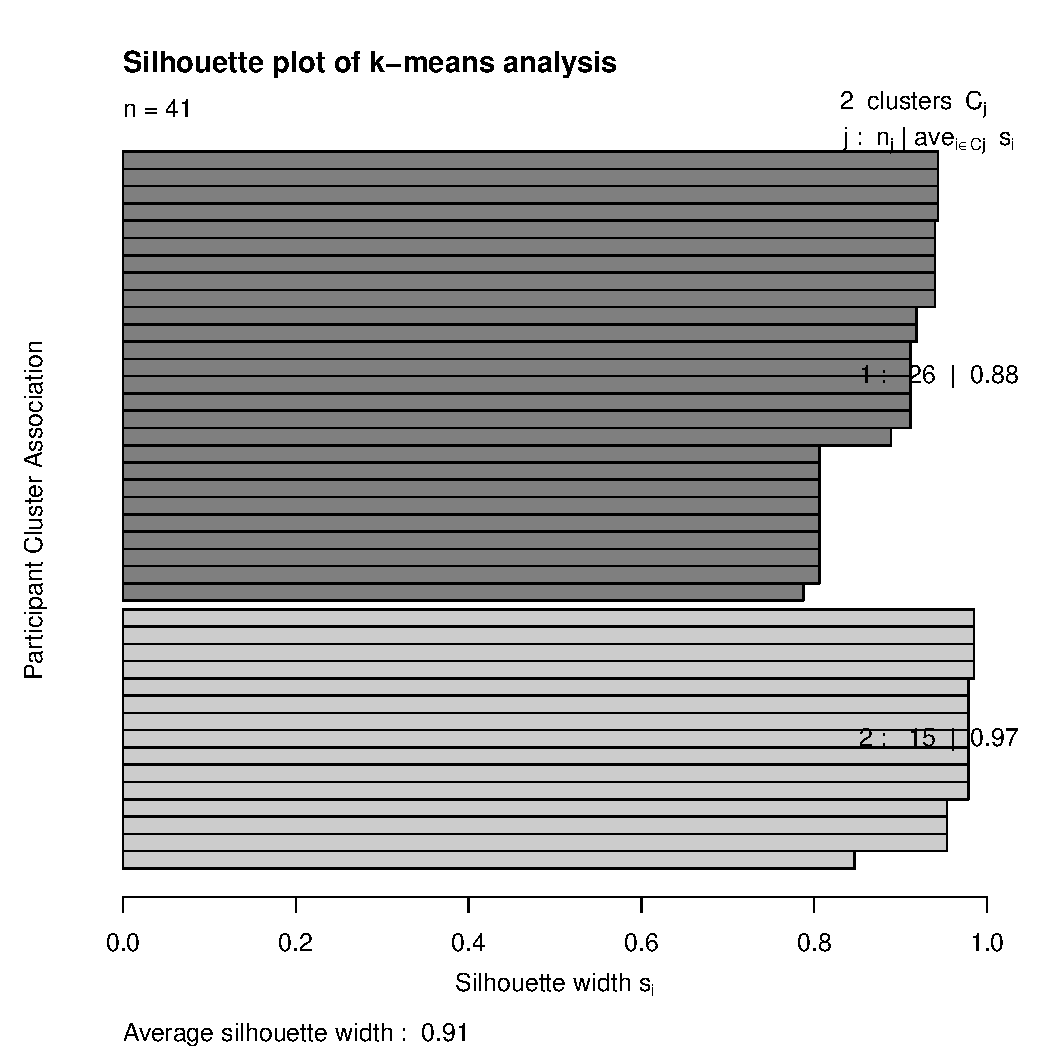
\includegraphics[width=0.69\linewidth]{silhouette.pdf}
    \caption{Silhouette plot of k-means analysis of participants by acceptability ratings}
    \labfig{silhouette plot}
\end{figure}

Subsequent one-tailed t-tests showed that there are no differences for each condition between population clusters except for the {\scshape dissimilar} condition with $t(69)=10.5, p<0.05$. For the {\scshape control} condition, we obtain $t(139)=-0.6, p>0.1$, for the {\scshape similar} condition, $t(69)=0.7, p>0.1$, and for the {\scshape disjoint} condition, $t(69)=0.3, p>0.1$.

For the {\scshape dissimilar} condition, the variance and acceptability is greatly reduced for Cluster 2, as shown in \reftab{average-results-pops} and \reffig{boxplot}:
\begin{table}[!htb]
    \caption{Average acceptability of each condition, divided by population cluster}
    \labtab{average-results-pops}
    \begin{tabular}{lrrrr}
    \toprule
        Condition & \multicolumn{2}{r}{Average Acceptability} & \multicolumn{2}{r}{Variance}\\\midrule
                        & Cluster 1       & Cluster 2       & Cluster 1 & Cluster 2\\\cmidrule[0.1pt](lr{0.1em}){2-3}\cmidrule[0.1pt](lr{0.1em}){4-5}
        {\scshape control}    & 1.50  & 1.44&   0.47      &  0.41\\
        {\scshape disjoint}   & 2.13  & 2.17 &   0.65     &  0.67\\
        {\scshape dissimilar} & 2.87  & 4.46 &   1.21     &  0.51\\
        {\scshape similar}    & 4.38  &   4.44  & 0.45  &  0.40\\
        \bottomrule
    \end{tabular}
\end{table}
\begin{figure}[!htb]
\begin{minipage}{\linewidth}
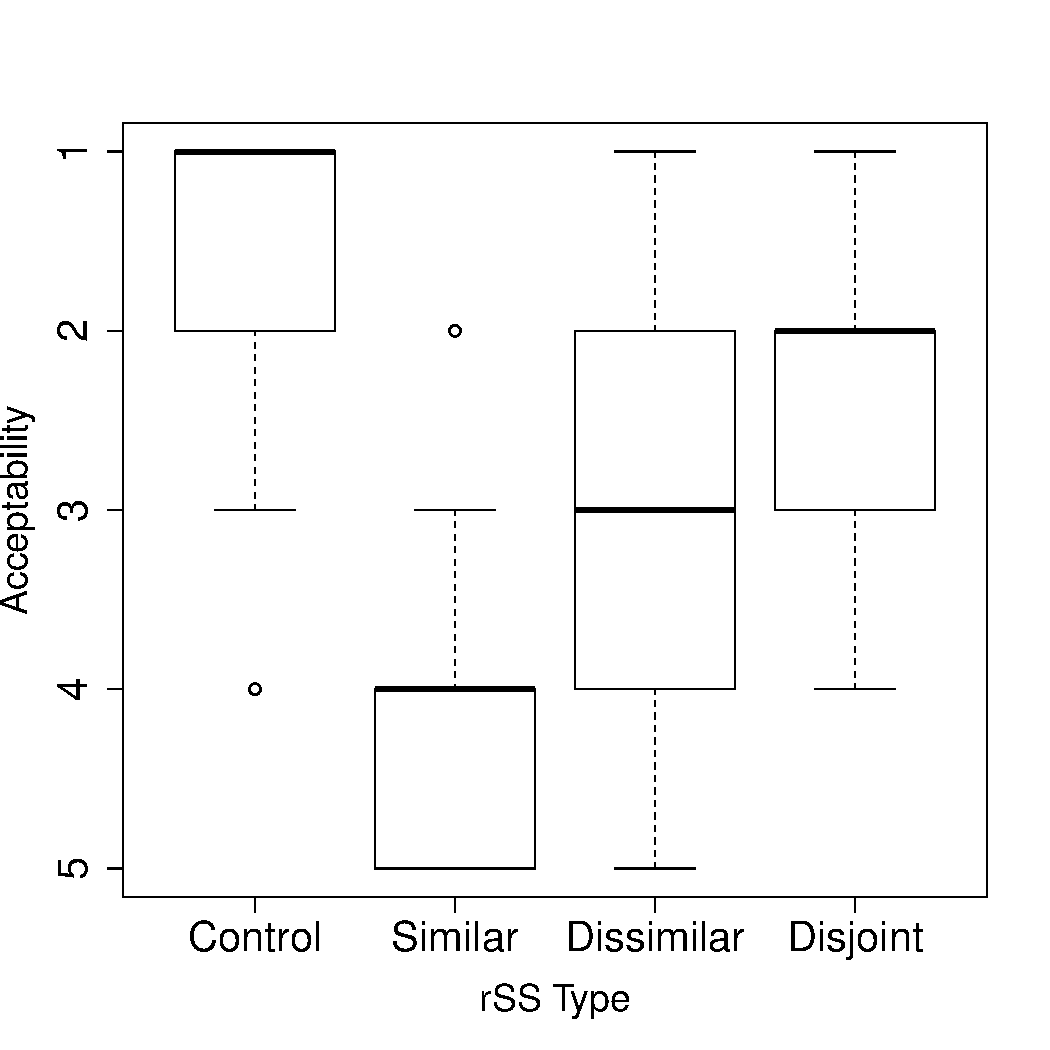
\includegraphics[page=1,width=0.425\linewidth]{boxplots.pdf}\hfill
\includegraphics[page=2,width=0.425\linewidth]{boxplots.pdf}
\end{minipage}
\caption{Boxplot for Cluster 1 (left) and Cluster 2 (right).}
\labfig{boxplot}
\end{figure}

One-tailed t-tests showed that, for Cluster 1, each condition is significantly different to every other condition. Comparing the {\scshape control} condition to the {\scshape disjoint} condition, we obtained $t(134)=-7.2, p<0.05$, to the {\scshape dissimilar} condition, $t(134)=-12.4, p<0.05$, and to the {\scshape similar} condition, $t(134)=-35.6, p<0.05$. Comparing the {\scshape similar} condition to the {\scshape dissimilar} condition, we obtain $t(134)=13.8, p<0.05$, and to the {\scshape disjoint} condition, $t(134)=23.6, p<0.05$. Comparing the {\scshape dissimilar} condition to the {\scshape disjoint} condition, we obtain $t(134)=6.4, p<0.05$.

For Cluster 2, the same one-tailed t-tests showed that each condition is significantly different to every other condition with the exception of the one-tailed t-test between {\scshape similarity} and {\scshape dissimilarity}, with $t(69)=-0.12, p>0.1$. Comparing the {\scshape control} condition to the {\scshape disjoint} condition, we obtained $t(69)=-5.1, p<0.05$, to the {\scshape dissimilar} condition, $t(69)=-23.6, p<0.05$, and to the {\scshape similar} condition, $t(69)=-27.7, p<0.05$. Comparing the {\scshape similar} to the {\scshape disjoint} condition, we obtained $t(69)=20.1, p<0.05$. Comparing the {\scshape dissimilar} condition to the {\scshape disjoint} condition, we obtain $t(69)=16.2, p<0.05$.


\subsection{Discussion}\labsec{discussion}
Our experiment set out to test two independent hypotheses, repeated below.
\begin{enumerate}
    \item If two reverse Sobel sequences are the same except for the degree of similarity between their conditionals' antecedent worlds, then the reverse Sobel sequence whose degree of similarity is more disparate should be considered more acceptable on average. (the \textit{dissimilar worlds hypothesis})
    \item If the domains of quantification of a reverse Sobel sequence are entirely disjoint, there should be no difference in acceptability between them and regular sentences (i.e. the control items). (the \textit{disjoint domain hypothesis})
\end{enumerate}
It is to be kept in mind that the second hypothesis mainly serves the purpose of establishing a positive baseline of acceptability for the results gathered from testing the first hypothesis.

\subsubsection{Disjoint Domain Hypothesis}\labsec{secondhypo}
Concerning the disjoint domain hypothesis, the results are quite clear: Since there is a significant difference between the {\scshape control} condition and the {\scshape disjoint} condition, and the latter is less acceptable on average, the null hypothesis has been falsified. However, the {\scshape disjoint} reverse Sobel sequences are, on average, only 0.67 points less acceptable than the control items. They are also far more acceptable than the other types of reverse Sobel sequences. We reckon that this slight---though significant---degradation in acceptability may be chalked up to the markedness of reverse Sobel sequences in general: The markedness of going from a specific case to a more general case that then seemingly contradicts the specific case, even if only on the surface. Generally speaking, in language, the reverse appears far more common (e.g. precisification). In the same line of reasoning, it appears, to us at least, quite difficult to find a natural occurrence of reverse Sobel sequences within any given corpus---written or spoken.

As such, we may consider the optimal reverse Sobel sequence acceptability to be below that of other, more typical utterances. The results of the dissimilar worlds hypothesis should therefore be contrasted against the results gathered from this hypothesis as a positive baseline, and not merely to the control items that consists of non-reverse Sobel sequences (amongst other utterance types).

\subsubsection{Dissimilar Worlds Hypothesis}\labsec{firsthypo}
For the dissimilar worlds hypothesis, the experiment yielded somewhat contradictory results. In \refsec{results}, it was shown that, for the undivided participant population, the {\scshape similar} condition is significantly different from the {\scshape dissimilar} condition and that the {\scshape dissimilar} condition yields higher values of acceptability than the {\scshape similar} condition by approximately one point of acceptability on average. As such, the hypothesis was technically confirmed, though the difference in acceptability was somewhat smaller and the variance of the {\scshape dissimilar} condition much higher than anticipated. However, the k-means cluster analysis has shown that there are actually two distinct population clusters within our group of participants. Cluster~1 continued to rate the {\scshape dissimilar} condition significantly higher in acceptability than the {\scshape similar} condition, now by approximately 1.5 points, but Cluster 2 appears to make no distinction between the two conditions whatsoever. Not only that, but the variance for the {\scshape dissimilar} condition in the first population cluster is still very high ($\sigma^2=1.21$) and the actual distribution of acceptability judgements disconcertingly even across the board, as seen in \reffig{boxplot}. As such, it seems that the participants in the first population cluster were unsure of what to do with these reverse Sobel sequence, rather than considering them a simple improvement on the {\scshape similar} condition's reverse Sobel sequence. Furthermore, both population clusters rate the {\scshape dissimilar} condition as less acceptable than the {\scshape disjoint} condition, meaning that even very dissimilar worlds do not automatically yield a reverse Sobel sequence whose acceptability rating could be considered as optimal.

These findings are unexpected by or contradictory to \citepos{Lewis2018} account, though to different degrees. If considered only on its own, Cluster 2 would directly falsify the dissimilar worlds hypothesis. The variance of Cluster 1 would suggest that dissimilarity---whilst clearly having a positive impact on acceptability in some cases---is not the sole deciding factor (aside from relevance) behind acceptability.

We must consider whether these two findings may be explained by \citepos{Lewis2018} model in its current state. Concerning Cluster 2, there are two explanations apparent to us: First, as the world closeness is an interaction between similarity and relevance, it might be the case that the participants of this population cluster consistently ascribe enough relevance to the $\phi\land\psi$-worlds s.t. they are always moved to be amongst the closest $\phi$-worlds irrespective of dissimilarity. The second possibility would be that they interpret the {\scshape dissimilar} $\phi\land\psi$-worlds as more similar than intended. The latter option would indicate that there might be an error in the experiment's design; more specifically, in how the {\scshape dissimilar} condition items were created. The former option would introduce the question why these participants would consistently go through the trouble of rearranging their world ordering -- even though most people would not, given the disparity in similarity -- if this leads to a contradictory reading. Both by principle of economy and charitability, it would be more suitable to leave the $\phi\land\psi$-worlds in their original place in the world ordering, given the vast distance they would have to cross to count amongst the closest $\phi$-worlds. Concerning the variance of the first population cluster, we have a similar option to argue in favour of \citepos{Lewis2018} model: If we were to assume that the $\phi\land\psi$-worlds of the {\scshape dissimilar} condition are regarded as more similar than intended, then the participants might be more inclined to provide them with lower acceptability ratings---the higher ratings would then be an act of charitable interpretation on their part. This would however raise the question why their charitability---a successful strategy---is only intermittently employed.

Excluding, for the sake of argument, the possibility of there being an inherent flaw in the design of the {\scshape dissimilar} reverse Sobel sequences and assuming that Cluster 2 is not that anti-charitable, we would argue that our results, whilst weakly supporting the dissimilar worlds hypothesis, are more contradictory to than supportive of \citepos{Lewis2018} model. Rather, the data would suggest to us that there is another main factor behind the acceptability of reverse Sobel sequence, as further explored in \refsec{introspection}.

\section{Felicity Factors for Reverse Sobel Sequences}\labsec{introspection}
In \refsec{firsthypo}, we argued that the experimental results suggest that relevance and dissimilarity may not be the only important factors for the acceptability of reverse Sobel sequences -- perhaps not even the main ones. What, then, renders reverse Sobel sequences acceptable in the rare instances when this is the case? From the results of the {\scshape disjoint} condition, we know that its ingredients are a recipe for (limited) success. Recalling the conditions for their creation from \refsec{materials}, we know them to be (i) establishing the $\phi\land\psi$-conditional as pertaining to epistemically excluded possibilities, whilst making the $\phi$-conditional a regular future-less-vivid conditional pertaining to live possibilities and (ii) having both sequence conditionals share a common discourse goal explicitly named by a sentence following the reverse Sobel sequence. As such, we tried to pin down what makes a reverse Sobel sequence acceptable by systematically creating reverse Sobel sequences with only one of these features or even neither of them whilst trying to keep the changes to a minimum. As we demonstrate on the following pages, native speaker acceptability judgements showed that (i) causal relations between the antecedent's propositions has the effect \textcite{Klecha2014} observed, (ii) reverse causal Sobel sequences are only felicitous if the relevance of $\phi\land\psi$ is denigrated or $\phi\land\psi$ is considered an epistemically excluded possibility, (iii) non-counterfactual reverse Sobel sequences are infelicitous unless the possibility of $\phi\land\psi$ is overtly denigrated, and that (iv) a unified discourse purpose is not required for felicity. 

First, we show that a unified discourse purpose is not required for felicity with the already existing example \refex{match}, repeated below as \refex{match-repeat3}:
\ex\phantomsection\context{Holding up a dry match, with no water around.}If I had struck this match and it had been soaked, it would not have lit. But if I \MakeUppercase{had} struck this match, it would have lit.\\%
\emptyfill(adapted from \textcite[p. 106]{Stalnaker1968} by \textcite[p. 487]{Lewis2018})\labex{match-repeat3}
\xe
Arguably, \refex{match-repeat3} is felicitous, even though there is no inherently clear discourse purpose shared by both conditionals. It could be argued that the shared purpose behind the sequence is to make the point that wet matches don't generally light when struck, but contexts are easily imaginable where the reverse Sobel sequence is merely uttered to reflect the reality of the match's dryness and what would have happened to it, if it had been struck. If this were to already count as a shared discourse purpose, it would be so broad in range that almost any non-incoherent discourse could be constructed as having a shared purpose in that sense, rendering it a non-factor anyhow.

Having excluded a shared discourse purpose as a relevant factor, we would posit the empirical breakdown in \reftab{ourdata}, where the corresponding example numbers that demonstrate this are given in brackets:%
\begin{table}[!htb]
\caption{Current empirical data on felicity distribution, broken down by causality, counterfactuality, and overt denigration of relevance (or implicit epistemic exclusion) of $\psi$, with example numbers that exemplify each reverse Sobel sequence condition. Contrastive stress on the auxiliary verb is assumed for all reverse Sobel sequences.}
\resizebox{\textwidth}{!}{
    \begin{tabular}{lcccccccc}\toprule
                &   \multicolumn{4}{c}{Acausal}     &  \multicolumn{4}{c}{Causal}\\
                & \multicolumn{2}{c}{Non-Counterfactual}  &   \multicolumn{2}{c}{Counterfactual}    & \multicolumn{2}{c}{Non-Counterfactual}  &   \multicolumn{2}{c}{Counterfactual}\\
                & Non-Denigrated & Denigrated  & Non-Denigrated & Denigrated   & Non-Denigrated & Denigrated & Non-Denigrated & Denigrated\\\midrule
          SS    &   \checkmark  & \checkmark &   \checkmark  &   \checkmark  &   \checkmark    &   \checkmark  &   \checkmark & \checkmark\\
          rSS   &   \#\refex{matchtomorrow}  & \checkmark\refex{acausalncfdenigrated}  & \checkmark\refex{match-repeat4}  &   \checkmark\refex{match-acausal-denigrated}  &   \#\refex{matchsnapnocf} & \checkmark\refex{causalncfdenigrated} &   \#\refex{matchsnapcf}    &   \checkmark\refex{match-causal-denigrated}\\
          \bottomrule
    \end{tabular}}\labtab{ourdata}
\end{table}

Crucially, it would appear that non-counterfactual and non-epistemically excluded possibility reverse Sobel sequences are typically infelicitous, as demonstrated with the reverse Sobel sequences in \refex{matchtomorrow} and \refex{matchsnapnocf}:
\ex\phantomsection\context{Concerning a dry match in a room with a large open source of water.}
    If I struck this match tomorrow and it was wet, it wouldn't light; \#but if I \MakeUppercase{were} to strike this match tomorrow, it would light.\labex{matchtomorrow}
\xe
\ex\phantomsection\context{Holding up a dry match (with no water around).}If I struck this match and it snapped, it would not light. \#But if I \MakeUppercase{were} to strike this match, it would light.\labex{matchsnapnocf}
\xe
This extends to all forms of non-counterfactual reverse Sobel sequences. As such, not only are future-less-vivid sequences infelicitous (as shown in \refex{matchtomorrow} and \refex{matchsnapnocf}), but their indicative counterparts as well, as shown in \refex{matchtomorrow-indicative} and \refex{matchsnapnocf-indicative}.
\ex\phantomsection\context{Concerning a dry match in a room with a large open source of water.}
    If I strike this match tomorrow and it is wet, it will not light; \#but if I \MakeUppercase{do} strike this match tomorrow, it will light.\labex{matchtomorrow-indicative}
\xe
\ex\phantomsection\context{Holding up a dry match (with no water around).}If I strike this match and it snaps, it will not light. \#But if I \MakeUppercase{do} strike this match, it will light.\labex{matchsnapnocf-indicative}
\xe

This may only be remedied by overtly questioning the relevance of $\phi\land\psi$ (or implicitly knowing of the quasi-impossibility and resulting irrelevance of $\psi$). If this is appropriately done, the reverse Sobel sequence is rendered felicitous, regardless of whether or not there is a causal relation between $\phi$ and $\psi$. This is demonstrated by \refex{acausalncfdenigrated}-\refex{causalncfdenigrated-indicative}.
\ex\phantomsection\context{Concerning a dry match in a room with a large open source of water.}
    If I struck this match tomorrow and it was wet, it wouldn't light. But there is little chance of this match becoming wet; so, if I \MakeUppercase{were} to strike this match tomorrow, it would light.\labex{acausalncfdenigrated}
\xe
\ex\phantomsection\context{Holding up a dry match (with no water around).}If I struck this match and it snapped, it would not light. But the chances of me snapping a match are really, really low; so, if I \MakeUppercase{were} to strike this match, it would light.\labex{causalncfdenigrated}
\xe
\ex\phantomsection\context{Concerning a dry match in a room with a large open source of water.}
    If I strike this match tomorrow and it is wet, it will not light. But there is little chance of this match becoming wet; so, if I \MakeUppercase{do} strike this match tomorrow, it will light.\labex{acausalncfdenigrated-indicative}
\xe
\ex\phantomsection\context{Holding up a dry match (with no water around).}If I strike this match and it snaps, it will not light. But the chances of me snapping a match are really, really low; so, if I \MakeUppercase{do} strike this match, it will light.\labex{causalncfdenigrated-indicative}
\xe

If a reverse Sobel sequence is counterfactual by nature, it would appear that they are always felicitous so long as $\phi$ and $\psi$ are causally unrelated (i.e., they are an acausal Sobel sequence), regardless of how dissimilar the worlds are to each other. This is demonstrated by \refex{match-repeat4} and \refex{match-similar}:
\ex\phantomsection\context{Holding up a dry match, with no water around.}If I had struck this match and it had been soaked, it would not have lit. But if I \MakeUppercase{had} struck this match, it would have lit.\\%
\emptyfill(adapted from \textcite[p. 106]{Stalnaker1968} by \textcite[p. 487]{Lewis2018})\labex{match-repeat4}
\xe
\ex\phantomsection\labex{match-similar}\context{Talking about a match that was dry but in a room with a large and open source of water; though the match did not get wet until being held by the speaker, it easily could have, had it moved even a little bit differently.}If I had struck this match and it had been soaked, it would not have lit. But if I \MakeUppercase{had} struck this match, it would have lit.
\xe

If there was some causal relation between $\phi$ and $\psi$, however, then, as \textcite{Klecha2014} already observed, the reverse Sobel sequence would be infelicitous, barring any intervention, as seen in \refex{matchsnapcf}:
\ex\phantomsection\context{Holding up a dry match (with no water around).}If I had struck this match and it had snapped, it would not have lit. \#But if I \MakeUppercase{had} struck this match, it would have lit.\labex{matchsnapcf}
\xe

Finally, causal and acausal reverse Sobel sequence may be rendered felicitous, if the relevance of $\phi\land\psi$ is appropriately denigrated via questioning its probability, as seen with the reverse Sobel sequences in \refex{match-acausal-denigrated} and \refex{match-causal-denigrated}:
\ex\phantomsection\context{Holding up a dry match, with no water around.}If I had struck this match and it had been soaked, it would not have lit. But, as we know, this match is dry, so if I \MakeUppercase{had} struck this match, it would have lit.\labex{match-acausal-denigrated}
\xe
\ex\phantomsection\context{Holding up a dry match (with no water around).}If I had struck this match and it had snapped, it wouldn't have lit. But the chances of the match breaking would've been very, very, \MakeUppercase{very} low, since I know what I'm doing. So, if I \MakeUppercase{had} struck this match, it would have lit.\labex{match-causal-denigrated}
\xe

With this, we may have identified the factor that threw off the results for the {\scshape similar} reverse Sobel sequences in \refsec{experiment}. In fact, considering the results from our experiment and that we have found no reverse Sobel sequences for which dissimilarity appears to play a role in felicity (short of the $\phi\land\psi$-worlds being so dissimilar that they ought to be considered excluded possibilities), we would argue that \citepos{Lewis2018} criterion of worlds having to be \enquote{similar enough} may be formally dropped: In the terminology of \textcite{Lewis2018}, any two sets of worlds appear similar enough so long as there is no counterfactuality or epistemically excluded possibility involved. Only if a reverse Sobel sequence involves a set of counterfactual or epistemically excluded worlds does similarity play a role in whether or not the sequence is rendered felicitous or infelicitous (in the sense of $\phi$ and $\phi\land\psi$ should not be equal in similarity). 

Having identified the criteria for reverse Sobel sequence felicity, we must now adopt some formal mechanism(s) whose predictions match the empirical data found within this chapter. We pursue this objective in \refch{pragmatics-SS}.
\cleardoublepage
\chapter{A Contrast-Based Model of Reverse Sobel Sequence (In-)Felicity}\labch{pragmatics-SS}
In the preceding chapter, we have isolated the criteria that render reverse Sobel sequences either felicitous or infelicitous. The pertinent data was gathered from the literature, an original experiment, and further introspection. The pertinent isolated empirical criteria are as follows: (i)~Contrastive stress in the second antecedent is required for felicity; (ii)~some form of stress obligatorily falls upon the auxiliary verb if no lexical item in the second conditional's antecedent is overtly different from the first conditional's antecedent; (iii)~despite assuming contrastive stress, a reverse Sobel sequence is always infelicitous, if the proposition $\phi$ precedes $\psi$ on some causal chain of events; (iv)~assuming felicity-enabling previous factors (including an acausal relationship between $\phi$ and $\psi$), a reverse Sobel sequence is always felicitous if the closest $\phi\land\psi$-worlds are counterfactual by nature; and (v)~assuming appropriate contrastive stress, the denigration of $\phi\land\psi$'s possibility renders any reverse Sobel sequence felicitous, regardless of all other previously mentioned factors (barring contrastive stress itself).%

To capture these intuitions, we propose to make use of the following ingredients and tools from the literature: (i)~The antecedent of a conditional sets the current aboutness topic \parencite{Ebert2008}, not only for indicative and future-less-vivid conditionals but also for counterfactual ones \parencite[cf.][p.~139]{Ebert2008}; (ii)~\textit{would} is sensitive to modal subordination \parencite{Klecha2011,Klecha2014,Klecha2015}; (iii)~the focus value for pro-forms may be a set of identity functions over alternative domains \parencite{Jacobson2004}; (iv)~differences to the actual world that causally stem from another initial change do not further decrease the similarity of the world in question \parencite{Bennett2003,Arregui2009}; (v)~imprecision and precisification may affect the evaluation of a conditional with respect to its set of antecedent worlds \parencite{Klecha2014,Klecha2015}; and (vi)~any domain of universal quantification is contextually restricted to exclude contextually irrelevant worlds \parencites{Fintel1994}{Reimer1998}{Stanley2000}{Klecha2014}[amongst many others]{Klecha2015}.

\section{The Effect of Contrastive Stress in a Variably-Strict Semantics}\labsec{contrast-vss}
The observation that some form of stress is required appears crucial: It is the only known factor that inevitably leads to infelicity should its requirement not be fulfilled. As such, the mechanisms surrounding contrastive stress must be at the centre of any explanation of reverse Sobel sequence (in-)felicity, including the one we present in this section.

As shown in \refsec{ASS}, there are two different strategies to derive a valid form of stress in the second conditional's antecedent of a reverse Sobel sequence: We either need to contrastively stress some lexical item that is overtly different from a counterpart in the preceding antecedent, or we have to stress the auxiliary verb of the reverse Sobel sequence's $\phi$-conditional. First, let us revisit the former case. Consider \refex{contrast-host}, repeated below as \refex{contrast-host-2}:
\pex\labex{contrast-host-2}\vspace{-9.5mm}
\a\speaker{Ben}If Karlos had hosted the party, it would not have been a good time.
\a\speaker{Martina}But if Karlos had \MakeUppercase{come} to the party, it would have been a good time.\hfill\parencite[p.~151]{Klecha2014}
\xe
As previously mentioned in \refsec{ASS}---as it was originally argued by \textcite[p.~52]{Klecha2014}---the contrastive stress on \textit{come} may lead to an exhaustified reading such as the one in \refex{contrast-host-exh}.
\pex
\a\speaker{Ben}If Karlos had hosted the party, it would not have been a
good time.
\a\speaker{Martina}But if Karlos had \MakeUppercase{come} to \textit{(but not hosted)} the party, it would have been a good time.\labex{contrast-host-exh}
\xe
Therefore, it is apparent why such reverse Sobel sequences might be felicitous: The set of the closest $\phi\land\psi$-worlds and the set of the closest $\phi\land\neg\psi$-worlds are, by definition, disjoint. This would prevent any inconsistent readings from arising from the semantics of the reverse Sobel sequence.

Now, let us revisit the second case: We have shown in \refsec{ASS} that some form of stress may occur even for reverse Sobel sequences where the second conditional's antecedent does not contain any lexical item that overtly differs from the first conditional's antecedent. In such cases, stress appears to obligatorily shift to the auxiliary verb, if present. The question would be why it is the auxiliary verb that is stressed. There appear to be three salient possibilities: 

First, an auxiliary verb is often contrastively stressed to contrast its clause's positive polarity against a preceding clause's negative polarity (see \citeauthor{Romero2004}, \citeyear{Romero2004}, p. 629; \citeauthor{Grimshaw2013}, \citeyear{Grimshaw2013}; \citeauthor{Wilder2013}, \citeyear{Wilder2013}; amongst others), as shown in \refex{positivepolarityfocus}
\ex
Everybody who didn't finish on time met with \MakeUppercase{John}, but everybody who \MakeUppercase{did} finish on {ti}me met with {Ma}ry.\\\emptyfill\parencite[adapted from][p.~630]{Romero2004}\labex{positivepolarityfocus}
\xe
It should be noted that---whilst the auxiliary verb is stressed to contrast positive polarity against negative polarity---the contrastive stress naturally falls upon the negation of its clause, if its negative polarity is to be contrasted against some preceding clause's positive polarity, as demonstrated by \refex{negativepolarityfocus}.
\ex
Everybody who finished on \MakeUppercase{ti}me met with \MakeUppercase{Ma}ry, and everybody who did \MakeUppercase{not} finish on time met with \MakeUppercase{John}.\hfill\parencite[p.~630]{Romero2004}\labex{negativepolarityfocus}
\xe
So, how does this fit into the antecedental stress exhibited by reverse Sobel sequences? It would seem that it does not. For starters, a reverse Sobel sequence does not exhibit a change in antecedent polarity between its $\phi\land\psi$-conditional and its subsequent $\phi$-conditional. The only difference is a difference in which worlds are explored and which consequences are predicted---there is no reason to assume that the $\phi$-conditional is contrasted against even an implicit $\neg\phi$-conditional. As such, we would rule out polarity focus as a potential option for reverse Sobel sequences.

Second, closely related to polarity focus, a stressed auxiliary verb may also signify verum focus \parencite{Hohle1992,Richter1993,Romero2004}. Contrary to the previous type of polarity focus, here, we do not contrast the positive polarity against a preceding clause's negative polarity, but rather emphasise that the speaker is certain that the proposition expressed by the clause should be added to the common ground \parencite{Hohle1992,Gutzmann2011,Romero2004,Romero2015,Gutzmann2020}. This intuition is shown in \refex{verumexample}, where the accented auxiliary verb appears to clarify the epistemic certainty of \textit{Kimiko went to the Himalayas}, after it was indirectly called into question by some previous speaker. In this sense, it is more akin to a contrast in epistemic certainty, rather than a contrast in polarity, compared to our examples \refex{positivepolarityfocus} and \refex{negativepolarityfocus}.
\pex\labex{verumexample}\vspace{-9.5mm}
\a \speaker{A} Peter claims Kimiko went to the Himalayas.\\
\speaker{S} She \MakeUppercase{did} go to the Himalayas.\\\emptyfill\parencite[adapted from][p.~630]{Romero2004}
\a \speaker{A} Peter doesn't think Kimiko went to the Himalayas.\\
\speaker{S} She \MakeUppercase{did} go to the Himalayas.\\\emptyfill\parencite[adapted from][p.~630]{Romero2004}
\xe
It is easy to see how a verum-based analysis might be attractive in terms of correctly deriving the (in-)felicity of certain reverse Sobel sequences: Let us assume that verum focus introduces a covert operator {\scshape verum}, as defined by \textcite{Romero2004}:
\ex
$\intension[gx/i]{{\scshape verum}\textsubscript{i}} = \lambda{p_{s,t}}.\lambda{w_s}.\forall{w'\in\text{Epi}_x(w)}[\forall{w''\in\text{Conv}_x(w')}[p\in CG_{w''}]]$
\xe
Here, $\text{Epi}_x(w)$ would be the set of worlds conforming to $x$’s knowledge in $w$; $\text{Conv}_x(w')$ is the set of worlds where all of $x$'s conversational goals in $w'$ are fulfilled (e.g., attaining maximal information whilst preserving truth); and where $\text{CG}_w''$ is the common ground; i.e.,~the set of propositions that the speakers assume in $w''$ to be true \parencite{Stalnaker1978}.

However, a {\scshape verum}-based analysis would present a number of issues: To know whether or not the stress on the auxiliary verb is actually a case of verum focus, we must look at the known effects of {\scshape verum} in the antecedents of conditionals. For example, \textcite[p.~533]{Romero2015} observed that {\scshape verum} appears to render conditionals that make use of counterfactual morphology to lead to a non-counterfactual conclusion (hereafter referred to as Anderson-style conditionals) infelicitous. This was demonstrated via two phenomena that, in conditionals, are nearly unambiguously known to be instances of {\scshape verum}: the particle \textit{really}---which is identical in meaning to {\scshape verum} \parencite[p.~625]{Romero2004}---and high negation in the antecedent. First, we demonstrate \citepos{Romero2015} observed effect of {\scshape verum} on Anderson-style conditionals with \textit{really} with the contrasting conditionals in \refex{anderson} and \refex{anderson-verum-really}:
\pex
\a If Jones had taken arsenic, he would have shown the symptoms that he indeed showed. So, it is likely that he took arsenic.\hfill\parencite{Anderson1951}\labex{anderson}
\a\ljudge{\#} If Jones really \MakeUppercase{had} taken arsenic, he would have shown the symptoms that he indeed showed. So, it is likely that he took arsenic.\labex{anderson-verum-really}
\xe
Second, we demonstrate \citepos{Romero2015} observed effect of {\scshape verum} on Anderson-style conditionals with high negation in the antecedent with the contrast between \refex{nevergonnausethisagain1} and \refex{nevergonnausethisagain2}:
\pex
\a If there hadn’t\textsubscript{Low} been any / had been no\textsubscript{Low} oil in the tank, the furnace would have made exactly the noise that it in fact did. So, it’s likely that the tank was empty.\hfill\parencite[p.~521]{Romero2015}\labex{nevergonnausethisagain1}
\a \ljudge{\#} If there hadn’t\textsubscript{High} been some\textsubscript{PPI} oil in the tank, the furnace would have made exactly the noise that it in fact did. So, it’s likely that the tank was empty.\hfill\parencite[p.~521]{Romero2015}\labex{nevergonnausethisagain2}
\xe
As such, if the stressed auxiliary verb in reverse Sobel sequences were to actually induce verum focus, it should follow that an Anderson-type reverse Sobel sequence should be infelicitous. However, if we consider the acausal counterfactual Anderson-type reverse Sobel sequence in \refex{anderson-rss}, this prediction does not bear out.
\ex\context{In a situation where the speaker tries to determine what caused Jones symptoms, where they disagree with another speaker's argument that arsenic could not be responsible if Jones was immune to its effects.}
Yes, if Jones had taken arsenic and he had been immune to its effects, he would not have shown the symptoms that he indeed showed; but if Jones \MakeUppercase{had} taken arsenic, he \MakeUppercase{would} have shown the symptoms that he indeed showed. So, it \MakeUppercase{is} likely that he \MakeUppercase{did} take arsenic.\labex{anderson-rss}
\xe
Therefore, we tentatively exclude verum focus as a possible candidate, as reverse Sobel sequences fail to pattern with other known cases of {\scshape verum}.%

The third focus option would be a contrastive tense-aspect-mood (hereafter TAM) focus, as is possible with stress on auxiliary verbs \parencite[p.~12f, footnote~3]{Goodhue2018}. Such contrastive focus is most frequently used to contrast a difference in tense: E.g., by emphasising that some proposition does not apply to the present, but to the past, as demonstrated by \refex{tensefocus}:
\pex
\speaker{A} Dinah is buying yogurt.\labex{tensefocus}
\a \speaker{B} No, she \MakeUppercase{was} buying yogurt.
\a \speaker{B} No, she (already) \MakeUppercase{did} buy yogurt.\\\emptyfill\parencite[p.~13, footnote~3]{Goodhue2018}
\xe
But how would this apply to reverse Sobel sequences? If we recall, the majority of reverse Sobel sequences use the same tense, aspect, and mood for both conditionals. Furthermore, most reverse Sobel sequences also refer to the same time interval, rather than, for example, two different points in the past. Instead, they rather refer to different possibilities for the same time interval---in the case of acausal counterfactual reverse Sobel sequences,  they refer to differently remote possibilities for the same time interval. Here, it is important to recall that TAM morphology in conditionals is connected to the properties of the world variable \parencites{Palmer1986}{Iatridou2000}{Arregui2009}{Romero2014}[amongst others]{Schulz2014}. We propose that the stress on the auxiliary verbs in reverse Sobel sequences targets exactly that part in meaning: the properties of the world variable $w$ which impact the quantificational domain of the conditional. If this is indeed the case, then \citepos{Klecha2014} general observation regarding the necessity of contrastive stress can be extended to these cases as well, and the underlying form of stress for all felicitous reverse Sobel sequences would be a form of contrastive stress/focus. However, before we further explore this concept in \refsec{proform}, we first take a look at modal subordination and aboutness topicality in \refsec{modal}.

\subsection{Modal Subordination}\labsec{modal}
First, we must answer the question of why reverse Sobel sequences tend to be infelicitous without contrastive stress, even if the two conditionals should, in theory, quantify over two differing levels of world closeness. Here, we would argue that \textcite{Klecha2014,Klecha2015} is correct with his suggestion that modal subordination might be the culprit.\footnote{Note that \textcite{Klecha2014,Klecha2015} only explicitly suggested modal subordination to apply to acausal reverse Sobel sequences. However, there is no reason not to apply it to all kinds of reverse Sobel sequences: After all, if \textit{would} is sensitive to modal subordination, it should occur regardless of causality.} That \textit{would} is actually sensitive to modal subordination is demonstrated by \refex{modalsubordination}, where the \textit{would} of the second sentence is interpreted with respect to the context established by the preceding sentence.
\ex 
My family used to go to Albion. We would drive through Ontario.\\\emptyfill\parencite[p.~378]{Klecha2011} \labex{modalsubordination}
\xe
\textcite{Klecha2014,Klecha2015} argues that this would affect the interpretation of a reverse Sobel sequence as follows: \enquote{If $\phi\land\psi$, $\neg\chi$; but if $\phi$, $\chi$} is interpreted as \enquote{If $\phi\land\psi$, $\neg\chi$; but if $\phi\land(\phi\land\psi)$, $\chi$}, which would render the $\phi$-conditional contradictory to the preceding $\phi\land\psi$-conditional. Essentially, this would mean that the $\phi$-conditional of a reverse Sobel sequence is interpreted with respect to the $\phi\land\psi$-conditional's domain of quantification, rather than establishing its own. 

First, we must ponder the question of when any conditional should be analysed with respect to a preceding conditional's antecedent: If we compare the subordinated example \refex{sobelesque} to the non-subordinated example \refex{nonsense-subordination}, there are two clear differences between them. 

\ex
\context{John is married to Mary. He is a good liar and a flirt. Because of this, Mary always suspected him of cheating and once contemplated hiring a very competent private investigator but ultimately decided against it. However, John has never actually cheated on Mary, unbeknownst to her. Sue knows all of this.}
\speaker{Sue}If John had cheated on Mary, she would've never found out about it; but if she had hired the private investigator, he would've brought her evidence of John's cheating.\labex{sobelesque}
\xe
\ex
\speaker{Sue}If John had killed his boss, he would've spent his summer in prison; but if John had won the lottery, he would've gone on a cruise around the world.\labex{nonsense-subordination}
\xe

The first difference is as follows: For \refex{sobelesque}, both conditionals appear to be topically related, as both can be interpreted as exploring the question of what would have happened had John cheated on his wife, going through different scenarios. For \refex{nonsense-subordination}, most people would have trouble coming up with a topical relation between the two conditionals: One explores what would have happened to John had he murdered his boss, whereas the other one explores what would have happened had he won the lottery.

The second difference is as follows: For \refex{sobelesque}, the consequent of the second conditional requires a modally subordinate reading. Without it, the conditional would be evaluated as false. For \refex{nonsense-subordination}, this is not the case. Traditional analyses would suggest, however, that modal subordination is not contingent upon the resulting reading's felicity \parencite{Roberts1987,Roberts1989}. Indeed, if we alter \refex{sobelesque} such that the second conditional's consequent is contradictory to the first conditional's antecedent, the modally subordinate reading appears to remain intact, yielding an infelicitous sequence, as seen below in \refex{sobelesque-bad}.
\ex
\context{John is married to Mary. He is a good liar and a flirt. Because of this, Mary always suspected him of cheating and once contemplated hiring a very competent private investigator but ultimately decided against it. However, John has never actually cheated on Mary, unbeknownst to her. Sue knows all of this.}
\speaker{Sue}If John had cheated on Mary, she would've never found out about it;\linebreak\ljudge{??} but if she had hired the private investigator, he would've told her that John didn't cheat on her.\labex{sobelesque-bad}
\xe
As such, modal subordination does not take into account whether or not its presence is advantageous or disadvantageous. Rather, modal subordination is solely determined by whether or not a conditional can be interpreted as topically related to the antecedent of its preceding conditional.

This observation fits well with \citepos{Ebert2008} claim that the antecedent of a conditional serves as an topic-introducing device. \textcite{Ebert2008,Ebert2014} argued that the antecedent of a fronted conditional sets the aboutness topic of the current discourse; i.e.,~it sets the topic by which the consequent is evaluated. We would argue that the first conditional's antecedent sets the aboutness topic as described by \textcite{Ebert2008,Ebert2014}, but that any subsequent conditional is interpreted as merely elaborating upon the previously established topic, if at all possible, thereby establishing a subordinating discourse relation between the two conditionals in question \parencite{Asher2005}.\footnote{An alternative approach in explaining this behaviour might lie with \textcite{Eckardt2021}, who proposes a DRT account which incorporates a world discourse referent that may be maintained over multiple sentences. We propose further research in that direction.}

This would explain (i)~why \refex{sobelesque} and \refex{sobelesque-bad} are modally subordinated, (ii)~why \refex{nonsense-subordination} is not, and (iii)~why reverse Sobel sequences are subjected to modal subordination by default: It is difficult to conceive that the $\phi$-antecedent's proposed topic could ever be considered incompatible to the pre-established aboutness topic of the $\phi\land\psi$-antecedent.

To establish a non-subordinating discourse relation in such cases, it would then appear necessary that the speaker provides some overt cue that clarifies that the new conditional should be interpreted with regards to its own particular aboutness topic, rather than the previously established one. We argue that this is accomplished via the contrastive stress that appears mandatory to felicitous reverse Sobel sequences. The reasoning concerning this is rather simple: Contrastive stress with regards to topic is referred to as contrastive topic in the literature \parencite{Buring1997,Buring2003,Krifka2007,Buring2016,Constant2012}, and contrastive topic, by definition, introduces a new topic that is clearly demarcated from any previous topic (that is, contrastive topic clarifies that its topic answers part of topical space that was hereto left unaddressed), cancelling the latter's actuality \parencite{Ebert2008,Krifka2007,Ebert2014,Lee2017,vanRooij2017,Yabushita2017} and thereby forces a non-subordinate discourse relation between itself and the previous sentence. \textcite[p.~44ff]{Krifka2007}, specifically, covers the use of contrastive topic for aboutness topics. An example of this is shown in \refex{krifka-cs}.
\pex\label{ex:krifka-cs}
\a \speaker{A}What do your siblings do?
\a \speaker{B}[My [\MakeUppercase{si}ster]\textsubscript{Focus}]\textsubscript{Topic} [studies \MakeUppercase{med}icine]\textsubscript{Focus},
and\\\phantom{\speaker{B}}[my [\MakeUppercase{bro}ther]\textsubscript{Focus}]\textsubscript{Topic} is [working on a \MakeUppercase{freight} ship]\textsubscript{Focus}.\\\emptyfill\parencite[adapted from][p.~44]{Krifka2007}
\xe
In order for the contrastive topic to be successful, however, we require that the two contrasted items do not topically overlap. E.g., for \refex{krifka-cs}, we would require that the topic of his sister and the topic of his brother are non-overlapping. If this is violated, as in \refex{krifka-cs-bad}, where the later topic is a subset of the earlier topic, its use is infelicitous.
\pex\label{ex:krifka-cs-bad}
\a \speaker{A}What do your siblings do?
\a \speaker{B}\phantom{\#}[My [\MakeUppercase{bro}thers]\textsubscript{Focus}]\textsubscript{Topic} [study \MakeUppercase{med}icine]\textsubscript{Focus},
and\\\phantom{\speaker{B}}\#[my [\MakeUppercase{lit}tle brother]\textsubscript{Focus}]\textsubscript{Topic} is [working on a \MakeUppercase{freight} ship]\textsubscript{Focus}.\\\emptyfill\parencite[p.~267]{Krifka2007}
\xe

In \refch{pragmatics-SS}, we have established that contrastive stress obligatorily falls upon the antecedent's auxiliary verb, should no other overtly different lexical item be available. Given reasoning concerning modal subordination above, we would assume that a contrastively stressed auxiliary verb must suffice to prevent a modally subordinate reading in order for such reverse Sobel sequences to be felicitous. Indeed, additional data supports the view that contrastive stress on the auxiliary verb cancels modally subordinate readings in conditionals. Compare \refex{sobelesque} and \refex{sobelesque-bad}, repeated below as respectively \hyperref[ex:nananana-batman1]{(\ref*{ex:nananana-batman1}-i)} and \hyperref[ex:nananana-batman1]{(\ref*{ex:nananana-batman1}-ii)}, to their respective counterparts in \hyperref[ex:nananana-batman3]{(\ref*{ex:nananana-batman3}-i)} and \hyperref[ex:nananana-batman3]{(\ref*{ex:nananana-batman3}-ii)}, where contrastive stress was added to the auxiliary verb.
\pex
\contextpex{John is married to Mary. He is a good liar and a flirt. Because of this, Mary always suspected him of cheating and once contemplated hiring a very competent private investigator but ultimately decided against it. However, John has never actually cheated on Mary, unbeknownst to her. Sue knows all of this.}
\a \pextitle{Without Contrastive Stress:}\beginsubsub
\b{i.} \speaker{Sue}If John had cheated on Mary, she would've never found out about it; but if she had hired the private investigator, he would've brought her evidence of John's cheating.\labex{nananana-batman1}
\b{ii.} \speaker{Sue}If John had cheated on Mary, she would've never found out about it; {??}but if she had hired the private investigator, he would've told her that John didn't cheat on her.\labex{nananana-batman2}
\endsubsub\pagebreak
\a \pextitle{With Contrastive Stress:}\beginsubsub
\b{i.} \speaker{Sue}If John had cheated on Mary, she would've never found out about it; {??}but if she \MakeUppercase{had} hired the private investigator, he would've brought her evidence of John's cheating.\labex{nananana-batman3}
\b{ii.} \speaker{Sue}If John had cheated on Mary, she would've never found out about it; but if she \MakeUppercase{had} hired the private investigator, he would've told her that John didn't cheat on her.
\endsubsub
\xe
Here, the acceptability of each sequence appears to be inverted by the introduction of contrastive stress\footnote{Again, it should be noted that the feedback I received on this from native speakers ($n=3$) was mixed. Whilst most considered the infelicitous sequences in \hyperref[ex:nananana-batman1]{(\ref*{ex:nananana-batman1}-ii)} and \hyperref[ex:nananana-batman3]{(\ref*{ex:nananana-batman3}-i)} significantly degraded, a minority found the sequence in \refex{nananana-batman3} only slightly less acceptable than \refex{nananana-batman1}. The trend appears clear regardless.}---which would be in line with a non-subordinated reading: After all, the private investigator cannot bring evidence of John's cheating if we do not carry over the previous conditional's counterfactual assumption that John had, in fact, cheated on Mary in \hyperref[ex:nananana-batman3]{(\ref*{ex:nananana-batman3}-i)}. As such, it is clear that a validly contrastively stressed auxiliary verb should suffice to prevent modal subordination within reverse Sobel sequences. However, not all contrastively stressed reverse Sobel sequences are actually felicitous. We must therefore face the question of what the formal semantics of contrastive stress in reverse Sobel sequences is---and how contrastive stress still derives infelicity in certain cases. We explore the former question in \refsec{proform}, before tackling the specifics of the latter question in \refsec{showitworks}.

\subsection{Auxiliary Verbs and the Focus Value of Pro-Forms}\labsec{proform}
In order to establish the felicity conditions for contrastive stress on auxiliary verbs, we must first take a look at the role auxiliary verbs play in the semantics of conditionals. At least in the English language, it is a generally uncontroversial claim to say that top-level auxiliary verbs encode the TAM information of their respective clause \parencites{Chomsky1957}{Akmajian1979}[amongst others]{Klein1994}, if present. It is furthermore generally accepted that TAM morphology is crucially connected to the domain world selection process of conditionals \parencites{Palmer1986}{Iatridou2000}{Arregui2009}{Romero2014}{Schulz2014}; e.g., by marking a conditional as either indicative, future-less-vivid, or counterfactual by nature. See the following minimal pair of example conditionals in \refex{kennedy}, due \textcite[p.~90]{Adams1970}:
\pex\label{ex:kennedy}
\a If Oswald didn't shoot Kennedy, someone else did.\labex{kennedy-indicative}
\a If Oswald hadn't shot Kennedy, someone else would have.\labex{kennedy-subjunctive}
\xe
The indicative in \refex{kennedy-indicative} makes an epistemic claim: The speaker may not be certain whether or not it was Oswald that shot Kennedy, but someones most certainly did. A statement that would be considered true by anyone who knows that Kennedy was, in fact, shot. The counterfactual subjunctive in \refex{kennedy-subjunctive}, on the other hand, makes a metaphysical claim about how the world would have worked: The speaker takes it for granted that it was, in fact, Oswald who shot Kennedy, but makes the claim that, had he not, someone else would have done so. Contrary to the indicative, this sentence would only be considered true by someone who believes that our world was structured in such a way that Kennedy's assassination was inevitable (e.g., by believing in a grand conspiracy or some such). As such, the TAM morphology---the only overtly differing factor between \refex{kennedy-indicative} and \refex{kennedy-subjunctive}---appears to impact the conditionals' domain of quantification: TAM morphology marks whether we quantify over a set of epistemic worlds or over a set of metaphysical worlds \parencite[see, amongst others,][p.~62]{Condoravdi2002}.


Despite a substantial amount of literature on the topic, there appear to be varying degrees of consensus on the specifics of the TAM morphology's semantic contribution; from which part of TAM semantics is actually present in any given conditional to which part of TAM morphology carries which specific semantics and what these specific semantics actually even are \parencite{Fintel1997,Fintel2001,Dudman1983,Dudman1984,Iatridou2000,Arregui2007,Anand2010,Schulz2014}. Originally, the semantics of TAM morphology was treated as a single, undifferentiated chunk \parencite{Stalnaker1975,Fintel1997}. Later work attempted to differentiate between the contribution of tense, mood, and aspect. Currently, the semantic contributions of aspect \parencite{Hacquard2006,Arregui2007,Anand2010} and mood \parencite{Romero2017}---for languages with proper mood---are relatively well-understood. Concerning tense, however, there are, at the moment, two different main lines of thought: One main line of thought is that tense morphology marks one form or another of \enquote{modal remoteness}, as pertaining to the world variable \parencite{Stalnaker1975,Palmer1986,Iatridou2000,Huddleston2002,Schulz2014}. In these cases, counterfactual TAM morphology may indicate that the antecedent worlds are not necessarily live possibilities of the conversants \parencite{Stalnaker1975,Fintel1997} or that the actual world is excluded from evaluation regardless of antecedent-compliance \parencite{Iatridou2000,Schulz2014}. The other main line of thought considers tense morphology to mark the \enquote{temporal remoteness} of the antecedent worlds---evaluating the conditional either with respect to present possibilities for non-counterfactual conditionals or with respect to possibilities of some earlier time for counterfactual conditionals \parencite{Dudman1983,Dudman1984,Ippolito2003,Arregui2009,Gronn2009,Romero2014,Romero2017}. For the purposes of this dissertation, we remain agnostic about the exact nature and distribution of the meaning of TAM morphology, but retain the common denominating factor---namely, that TAM morphology restricts and selects the set of evaluation worlds from the set of all compatible antecedent worlds in one way or another.

In reverse Sobel sequences, the TAM morphology of the auxiliary verbs would yield different semantic values that could be contrasted against: One auxiliary verb's TAM morphology restricts the domain of quantification to the closest $\phi\land\psi$-worlds, whereas the other auxiliary verb's TAM morphology restricts the domain of quantification to the closest $\phi$-worlds. As these two sets should always be non-identical so long as $\phi\neq\psi$, one could argue that the contrast should always succeed and that any reverse Sobel sequence with contrastive stress on the auxiliary verb be rendered felicitous (barring other intervening factors). It would appear, however, that non-identicality is insufficient, considering the plenitude of infelicitous reverse Sobel sequences seen in \refsec{introspection} (e.g., non-denigrated counterfactual causal reverse Sobel sequences and non-denigrated non-counterfactual reverse Sobel sequences are infelicitous regardless of contrastive stress). It would appear that the two contrasting domains must not only be non-identical but rather entirely disjoint for a successful contrast (as the reverse Sobel sequence would yield a logical contradiction otherwise). As such, we require a semantic mechanism that ideally not only enforces non-identicality but also facilitates disjointness to escape modal subordination and to thereby also escape contradictory readings. In other words, we require the $\phi$-conditional to be interpreted as using a $\phi\land\neg\psi$-domain (without overtly placing the $\neg\psi$ in the antecedent) to be disjoint to the preceding $\phi\land\psi$-domain. We previously saw this facilitated in, e.g., \refex{match}, repeated below as \refex{match-s2-repeat}, where the second antecedent is interpreted as restricting our claim to worlds in which the speaker had struck the match and where we maintain the fact that the match was dry.
\ex\labex{match-s2-repeat}\context{Holding up a dry match, with no water around.}If I had struck this match and it had been soaked, it would not have lit. But if I had struck this match, it would have lit.\\%
\emptyfill(adapted from \textcite[p.~106]{Stalnaker1968} by \textcite[p.~487]{Lewis2018})
\xe

In this regard, reverse Sobel sequences behave strikingly similar to contrastively stressed bound pro-nouns, which also not only require non-identical contrasting domains, but contrasting domains that are, in fact, disjoint \parencite{Sauerland1998,Sauerland1999,Sauerland2000,Jacobson2000,Jacobson2004,Mayr2012}. Therefore, we would argue that a successful analysis of contrastively stressed TAM moprhology patterns along the lines of analyses regarding contrastively stressed bound pro-forms.

To this end, we make a brief excursion to the semantics of bound pronouns with contrastive stress: \textcite{Sauerland1998,Sauerland1999} argued for the existence of indices in the grammar using sentences such as \refex{sauerland}, where bound pronouns were focused via contrastive stress.
\ex
Every fourth grade boy$_i$ called his$_i$ mother, but no \MakeUppercase{fifth} grade boy$_j$ called \MakeUppercase{his}$_j$ mother.\labex{sauerland}
\xe
However, as noted by \textcite{Jacobson2000,Jacobson2004} and \textcite{Sauerland2000} himself, this does not appear to be a case of simply contrasting differing indices: Contrastively bound pronouns appear to be illicit when their binders may be different but still overlapping in their domain, as demonstrated by \refex{sauerland-domain}.
\ex
\ljudge{*}I expected every student\textsubscript{i} to call his\textsubscript{i} father, but only every \MakeUppercase{young} student\textsubscript{j} called \MakeUppercase{his}\textsubscript{j} father.\hfill\parencite[p.~206]{Sauerland1998}\labex{sauerland-domain}
\xe
\textcite{Jacobson2000,Jacobson2004} used this to argue for an alternate analysis of focused pronouns: She argues that contrastively stressed pronouns may give rise to two different sets of alternatives:  When not contrasted against another bound pronoun, the set of alternatives typically consists of the pronoun function from an individual to self (i.e.,~the identity function) and functions that map that individual to someone else, deriving a contrast this way. An example of such a case can be seen in \refex{jacobson-contrast-identity}.
\ex
Every fourth grade boy loves Jack's mother, and every fifth grade boy$_j$ loves \MakeUppercase{his}$_j$ mother.\labex{jacobson-contrast-identity}
\xe
When a pronoun is contrasted against another bound pronoun, the set of alternatives consists of (partial) identity functions of different domains, mapping elements of their restricted domain to themselves, deriving an obligatory contrast in domains between the two pronouns.
\pex
\a $\intension[g,c]{his\textsubscript{1}}$ is defined if $g(1)\in{D_R}$, where $D_R$ is the domain that binds the pronoun. When defined, $\intension[g,c]{his\textsubscript{1}}=g(1)$.
\a $\intension[g,c]{his\textsubscript{1}}=\predicate{id\textsubscript{R}}(g(1))$
\a $\intension[f,g,c]{his\textsubscript{1}}=\{\predicate{id\textsubscript{R'}}(g(1))~|~\predicate{id\textsubscript{R'}}\subseteq \predicate{id}_{\langle e,e\rangle}\}$
\xe
Crucially, \textcite{Jacobson2000,Jacobson2004} posits that the two contrasting (partial) identity functions' domains of definition must be non-overlapping (i.e.,~there is no element that is mapped by both identity functions to either itself or any other defined value). An unsuccessful example of this type of contrast was already shown in \refex{sauerland-domain}, where one domain was the subset of the other, and a successful example of this type of contrast was shown in \refex{sauerland}. The corresponding LFs are shown in \refex{jacobsonex2}, where the contrasting elements are highlighted in boldface.
\pex\label{ex:jacobsonex2}
\a every 3\textsuperscript{rd}-grader $[\lambda x.\predicate{call}(x, \predicate{the-mother-of}(\predicate{\textbf{\color{black}id\textsubscript{3rd-graders}}}(x)))]$
\a every 4\textsuperscript{th}-grader $[\lambda x.\predicate{call}(x, \predicate{the-mother-of}(\predicate{\textbf{\color{black}id\textsubscript{4th-graders}}}(x)))]$
\xe

\textcite{Jacobson2000,Jacobson2004} further argues for the existence of these two readings using sentences where contrastive stress is placed upon a reflexive pronoun, where the two different readings manifest themselves as variant stress patterns: If the contrast between the mapping from an individual to self vs. others is desired, the contrastive stress falls upon the \textit{self} of the reflexive pronoun, as shown in \refex{identity-good}. If, on the other hand, the contrast between domains is required, then the contrastive stress falls upon the pro-form part of the reflexive pronoun, as shown in \refex{domain-good}.
\pex
\a Every third grade boy loves Mary, and every \MakeUppercase{fourth} grade boy loves him\MakeUppercase{self} (as opposed to someone else). \labex{identity-good}
\a Every third grade boy loves himself, and every \MakeUppercase{fourth} grade boy loves \MakeUppercase{him}self \labex{domain-good}
\emptyfill\parencite[adapted from][p.~68]{Jacobson2000}
\xe
This placement of contrastive stress appears obligatory, as using the opposite stress pattern for either case would yield illicit readings, as shown in \refex{identity-bad} and \refex{domain-bad}.
\pex
\a\ljudge* Every third grade boy loves Mary, and every \MakeUppercase{fourth} grade boy loves \MakeUppercase{him}self.\labex{domain-bad}
\a\ljudge* Every third grade boy loves himself, and every \MakeUppercase{fourth} grade boy loves him\MakeUppercase{self} (*as opposed to someone else).\labex{identity-bad}\\
\emptyfill\parencite[adapted from][p.~68]{Jacobson2000}
\xe
Of these two readings, only the contrast in domains is of any relevance to the topic of reverse Sobel sequences---we would, therefore, refer to \textcite{Jacobson2000} for information on the other type of contrast.

How does this relate to the contrastive stress placed upon the auxiliary verb for reverse Sobel sequences? As previously stated, we would argue that contrastive stress or focus on an antecedent's auxiliary verb's TAM morphology evokes a value akin to bound pronouns that are contrastively stressed against another bound pronoun. Tense, for example, is often treated as a type of pro-form, as shown in \refex{tense}---e.g., by \textcite{Partee1973} and \textcite{Kratzer1998} amongst many others.
\ex 
$\intension[g,c]{\scshape past\textsubscript{i}}$ is defined only if $g(i)$ temporally precedes $t_0$, where $g(i)$ refers to the event time and $t_0$ refers to the actual time.\footnote{This definition corresponds to an absolute tense reading for the sake of simplicity. For a relative treatment of tense, see \textcite{Kusumoto1999}.}\\If defined, $\intension[g,c]{\scshape past\textsubscript{i}}=g(i)$\hfill\parencite[adapted from][p.~378]{Romero2017}.\labex{tense}
\xe
In addition, mood has also been treated as a type of pro-form in the literature, as shown in \refex{mood}---e.g., by \textcite{Schlenker2004,Schlenker2005}, who treated mood as pro-worlds.
\ex
$\intension[g,c]{\scshape indicative\textsubscript{i}}$ is defined only if $g(i)\in\predicate{dox\textsubscript{speaker}}$, where $\predicate{dox\textsubscript{speaker}}$ is the speaker's doxastic set of possible worlds.\\If defined, $\intension[g,c]{\scshape indicative\textsubscript{i}}=g(i)$\hfill\parencite[adapted from][p.~379]{Romero2017}.\labex{mood}
\xe
Now, in relation to reverse Sobel sequences, we would argue that focus on TAM-inflected verbs does not yield a set of alternative TAM-inflected verbs but rather a set of alternative domains---i.e.,~focus actually targets the domains of bound pronouns and the inflected TAM morphology rather than the focused items' stem meanings themselves. %
Let us recall that TAM morphology appears to be (at least partially) responsible for the world selection function of conditionals. As such, a contrastively stressed TAM verb should generate a set of salient alternative domain assignments that could, conceivably, have been used in place of the original conditional's domain of quantification. We show this is \refdef{tam}.
\pex\label{def:tam}
\a $\intension[g,c]{TAM\textsubscript{i}}$ is defined if $g(i)\in{D_R}$, where $D_R$ is the domain that binds the pro-form. When defined, $\intension[g,c]{TAM\textsubscript{i}}=g(i)$.
\a $\intension[g,c]{TAM\textsubscript{i}}=\predicate{id\textsubscript{R}}(g(i))$
\a $\intension[f,g,c]{TAM\textsubscript{i}}=\{\predicate{id\textsubscript{R'}}(g(i))~|~\predicate{id\textsubscript{R'}}\subseteq \predicate{id}_{\langle s,s\rangle}\}$
\xe
This set of alternatives would include the domain that it is contrasted against, as well as containing a number of less maximally similar antecedent compatible worlds. We also posit a presupposition to the contrastive stress that the two contrasting domains must be disjoint, inheriting this presupposition from the analysis of contrastively stressed bound pro-forms.\footnote{Note that whilst \textcite{Jacobson2000,Jacobson2004} herself does not provide an independent analysis for as to why disjoint domains should be required, there have been formal models that attempt to do so. We would refer to \textcite[p.~321 ff.]{Mayr2012} for one such account. We content ourselves with a simple presupposition of disjointness here, since the exact implementation that derives the requirement of disjoint domains is of no further consequence to the overall analysis.}

Having established what the alternatives to the auxiliary verb might be and what is required for a felicitous contrast, we may turn our attention to how the contrastive stress affects a reverse Sobel sequence: For the sequence \enquote{If $\phi\land\psi$, $\neg\chi$; but if {\scshape aux}\textsubscript{\scshape ct}-$\phi$, $\chi$}, the contrastive stress would attempt to contrast the set of the closest $\phi$-worlds against the salient counterpart of the preceding conditional: the set of the closest $\phi\land\psi$-worlds. As previously mentioned, due to the nature of the contrast, we would require the two contrasting domains to be disjoint. This is only the case if the $\phi$-conditional does not quantify over any of the closest $\phi\land\psi$-worlds, which, in turn, may only be the case---given a standard variably-strict analysis---if the two domains represent subsets of differing levels of world closeness. The respective LFs for a standard reverse Sobel sequence would therefore correspond to the LFs display in \refex{identityw}, where the contrasting identity functions are highlighted in boldface:
\pex\label{ex:identityw}
\a If $[\lambda w_s. \phi(\text{\textbf{\color{black}\scshape id\textsubscript{domain-b}}}(w))\land \psi(\text{\color{black}\scshape id\textsubscript{domain-b}}(w))]$, (then) $[\lambda w_s.\neg\chi(w)]$.
\a If $[\lambda w_s. \phi(\text{\textbf{\color{black}\scshape id\textsubscript{domain-a}}}(w))]$, (then) $[\lambda w_s.\chi(w)]$.
\xe
Where, as previously stated, in a variably-strict semantics domain A and domain B would correspond to the set of the closest $\phi$-worlds and the set of the closest $\phi\land\psi$-worlds, respectively, as shown in \refex{identityw-variably-strict}.
\pex\label{ex:identityw-variably-strict}
\a If $[\lambda w_s. \phi(\text{\textbf{\color{black}\scshape id\textsubscript{closest-$\phi\land\psi$}}}(w))\land \psi(\text{\color{black}\scshape id\textsubscript{closest-$\phi\land\psi$}}(w))]$, (then) $[\lambda w_s.\neg\chi(w)]$.
\a If $[\lambda w_s. \phi(\text{\textbf{\color{black}\scshape id\textsubscript{closest-$\phi$}}}(w))]$, (then) $[\lambda w_s.\chi(w)]$.
\xe
The formal implementation of which is shown in \refex{identityw-variably-strict-demo}, where the accessibility function $f_\leqslant(p,w)$ returns the set of $p$-worlds closest to the evaluation world $w$.
\pex\label{ex:identityw-variably-strict-demo}
\a $\intension{If $\phi$ and $\psi$, not $\chi$}=[\lambda w_s.\forall v:v\in f_\leqslant([\lambda w'_s.\phi(\text{\textbf{\color{black}\scshape id\textsubscript{closest-$\phi\land\psi$}}}(w'))$\\\emptyfill$\land\psi(\text{\textbf{\color{black}\scshape id\textsubscript{closest-$\phi\land\psi$}}}(w'))],w)[\neg\chi(v)]]$
\a $\intension{If $\phi$, $\chi$}=[\lambda w_s.\forall v:v\in f_\leqslant([\lambda w'_s.\phi(\text{\textbf{\color{black}\scshape id\textsubscript{closest-$\phi$}}}(w'))],w)[\chi(v)]]$
\xe

With this, we have established the felicity conditions for reverse Sobel sequences where the TAM-inflected verb is contrastively stressed---and thereby determined the factor that dictates whether or not modal subordination can be escaped: disjoint quantificational domains. The specifics on which reverse Sobel sequences fulfil these conditions are treated in the next section---i.e.,~\refsec{showitworks}.




But first, to summarise our position: We posit (i)~that the antecedent of a conditional sets the aboutness topic of the current discourse \parencite{Ebert2008,Ebert2014}; (ii)~that, in a sequence of conditionals, non-initial conditionals do not replace the established aboutness topic if there is some sensible way for their antecedent to correlate to it---causing non-initial conditionals to be analysed as modally subordinate to said aboutness topic; (iii)~that, if this is the case, contrastive stress is required as a cue to terminate the current aboutness topic and establish a new one---thereby cancelling modally subordinate readings (as motivated in \refsec{modal}); and (iv)~that contrastive TAM stress in the antecedent of conditionals is only felicitous if the contrasting conditionals' domains of quantification are disjoint to one another (as motivated in this section). In addition to what we have established in these sections, we also posit (v)~\citepos{Klecha2014,Klecha2015} model on causal Sobel sequences, including a world similarity metric \`a la \textcite{Bennett2003} and \textcite{Arregui2009}, as described in \refsec{CSS}; and (vi)~that domains of quantification are contextually restricted to exclude all worlds that are considered irrelevant to the discourse purpose \parencites{Fintel1994}{Reimer1998}{Stanley2000}{Klecha2014}[amongst many others]{Klecha2015}. We show in \refsec{showitworks} that these assumptions suffice to account for all known data presented in \refsec{introspection}, allowing for a uniform analysis of all felicitous reverse Sobel sequences assuming a single type of stress/focus in the antecedent of the second conditional.

\subsection{Retrodiction: Accounting for All Available Data With a Variably-Strict Semantics}\labsec{showitworks}
In order to test whether or not the model posited in \refsec{modal} and \refsec{proform} makes accurate predictions concerning the (in-)felicity of reverse Sobel sequences and regularly ordered Sobel sequences, we must first recall two important patterns of (in-)felicity: First, that all regularly ordered Sobel sequences are felicitous. Second, that the felicity of reverse Sobel sequences is dependent upon contrastive stress and three subordinate factors: causality, counterfactuality, and denigration. We established and summarised this in \refsec{introspection} in \reftab{ourdata}, repeated below as \reftab{ourdata-repeat}.

\begin{table}[!htb]
\caption{Current empirical data on felicity distribution, broken down by causality, counterfactuality, and overt denigration of relevance (or implicit epistemic exclusion) of $\psi$, with example numbers that exemplify each reverse Sobel sequence condition. Contrastive stress on the auxiliary verb is assumed for all reverse Sobel sequences.}
\resizebox{\textwidth}{!}{
    \begin{tabular}{lcccccccc}\toprule
                &   \multicolumn{4}{c}{Acausal}     &  \multicolumn{4}{c}{Causal}\\
                & \multicolumn{2}{c}{Non-Counterfactual}  &   \multicolumn{2}{c}{Counterfactual}    & \multicolumn{2}{c}{Non-Counterfactual}  &   \multicolumn{2}{c}{Counterfactual}\\
                & Non-Denigrated & Denigrated  & Non-Denigrated & Denigrated   & Non-Denigrated & Denigrated & Non-Denigrated & Denigrated\\\midrule
          SS    &   \checkmark  & \checkmark &   \checkmark  &   \checkmark  &   \checkmark    &   \checkmark  &   \checkmark & \checkmark\\
          rSS   &   \#\refex{matchtomorrow}  & \checkmark\refex{acausalncfdenigrated}  & \checkmark\refex{match-repeat4}  &   \checkmark\refex{match-acausal-denigrated}  &   \#\refex{matchsnapnocf} & \checkmark\refex{causalncfdenigrated} &   \#\refex{matchsnapcf}    &   \checkmark\refex{match-causal-denigrated}\\
          \bottomrule
    \end{tabular}}\labtab{ourdata-repeat}
\end{table}

\noindent Due to the greater theoretical importance of reverse Sobel sequence compared to regularly ordered Sobel sequences, we first tackle the (in-)felicity conditions of the former and then proceed to tackle the general felicity of the latter.

\subsubsection{Reverse Sobel Sequences}\labsec{vs-retro-rss}
In \refsec{modal}, we have argued that modal subordination is the default for all reverse Sobel sequences, leading to a contradictory reading due to both conditional antecedents quantifying over the same domain of worlds, and that reverse Sobel sequences require a successful contrastive stress in the antecedent to escape the subordinate reading, and thereby escape the contradictory reading cause by modal subordination. As argued for in \refsec{proform}, in order for the contrastive stress to be successful, we must be able to construct a domain that is disjoint from the preceding conditional's domain of quantification. Or, in set theoretical terms, contrastive stress on the auxiliary verb of a reverse Sobel sequence is felicitous iff $D_1\cap D_2=\emptyset$, where $D_1\subseteq D_{\text{closest-}\phi}$ and $D_2\subseteq D_{\text{closest-}\phi\land\psi}$. Here, $D_{\text{closest-}\phi}$ refers to the domain of worlds consisting of all maximally close $\phi$-worlds and $D_{\text{closest-}\phi\land\psi}$ refers to the domain of worlds consisting of all maximally close $\phi\land\psi$-worlds.

First, let us examine the effect of counterfactuality of $\phi\land\psi$ (note that we loop back to the effect of non-counterfactuality only later on). The example reverse Sobel sequences contrasting non-counterfactual ones with counterfactual ones, \refex{matchtomorrow} and \refex{match-repeat4}, are repeated below as \refex{doomsday-x} and \refex{doomsday-y}, respectively.
\ex\context{Concerning a dry match in a room with a large open source of water.}
    If I struck this match tomorrow and it was wet, it wouldn't light; \#but if I \MakeUppercase{were} to strike this match tomorrow, it would light.\labex{doomsday-x}
\xe
\ex\context{Holding up a dry match, with no water around.}If I had struck this match and it had been soaked, it would not have lit. But if I \MakeUppercase{had} struck this match, it would have lit.\\%
\emptyfill(adapted from \textcite[p.~106]{Stalnaker1968} by \textcite[p.~487]{Lewis2018})\labex{doomsday-y}
\xe
Our prime directive is to ensure the disjointness of the two domains of quantification. In the case of counterfactuality, it can be easily guaranteed that two domains of quantification are disjoint. For this to be the case, $\phi\land\psi$ and $\phi$ merely must possess differing degrees of similarity to the evaluation world to ensure that the closest $\phi$-worlds are $\phi\land\neg\psi$-worlds, since the world closeness ordering of counterfactual worlds is a mostly immutable system\footnote{With standard variably-strict semantics in the tradition of \textcite{Stalnaker1968} and \textcite{Lewis1973}, given a world similarity metric in the tradition of \textcite{Bennett2003} or \textcite{Arregui2009}, the only way to affect the world closeness of counterfactual worlds is to reevaluate either the counterfactuality or the causal relatedness of the corresponding counterfactual propositions.} that is determined solely by cause-initial deviances to the evaluation world (i.e.,~deviances to the evaluation world that do not causally follow from another deviance to the evaluation world). As such, two domains with differing degrees of counterfactual world closeness may definitively be considered disjoint for all discourse participants---thereby allowing for the possibility of a successful contrastive stress between them. Whether or not the two domains are actually disjoint depends on whether or not there is some causal link between $\phi$ and $\psi$, leading us to the next felicity factor of reverse Sobel sequences: the causal or acausal relationship between $\phi$ and $\psi$.

As extensively covered in \refsec{CSS}, assuming a world similarity metric in the spirit of \textcite{Bennett2003} and \textcite{Arregui2009} would postulate that the closest $\phi\land\psi$-worlds and the closest $\phi$-worlds are equal in similarity if $\phi$ precedes $\psi$ on some causal chain of events. As such, the worlds quantified over by the $\phi\land\psi$-conditional of a causal reverse Sobel sequence would merely constitute a subset of the worlds quantified over by the subsequent $\phi$-conditional. This is illustrated in \reffig{klecha-causal-rss-mystuff}.
\begin{figure}[!htb]
\input{content/graphics/klecha-causal-rSS.tikz}
\caption{Quantificational domains for reverse counterfactual causal Sobel sequences, where antecedent worlds are in boldface, and where $\phi$ precedes $\psi$ on some causal chain of events. For all worlds $w_n$: If $n\geqslant1$, then $\phi=1$ is true for $w_n$, and if $n\geqslant 4$, then $\psi=1$ holds true for $w_n$. If $n\geqslant 7$, then some proposition $\omega=1$ such that $\omega\neq\phi$, $\omega\neq\psi$, and $\phi,\psi$ do not precede $\omega$ on some causal chain of events.}\labfig{klecha-causal-rss-mystuff}
\end{figure}

\noindent Here, the $\phi\land\psi$-conditional and the $\phi$-conditional quantify over the same degree of world closeness (the shaded sphere in grey), as they are considered equal in similarity to the evaluation world due to the causal link between $\phi$ and $\psi$ \parencite{Bennett2003,Arregui2009}. As such, the $\phi\land\psi$-conditional quantifies over a subset of the $\phi$-conditional's antecedent worlds---as they are equal in world closeness, but not necessarily equal in the total number of worlds quantified over due to former's added constraint of them being $\psi$-worlds as well as $\phi$-worlds (a property that is only fulfilled by $w_4$, $w_5$, and $w_6$ for that degree of world closeness in \reffig{klecha-causal-rss-mystuff}). The $\phi$-conditional, quantifying over the worlds $w_1$ to $w_6$, would then make a contradictory claim regarding the status of $\chi$ in these shared worlds---which is unavoidable due to the effect of causality on world similarity.

As such, any contrastive stress that attempts to contrast the two world domains would fail, since the domains in question are not at all disjoint, as would be required for a valid contrast. Or, put in set theoretical terms, since $D_{\text{closest-}\phi\land\psi}\subseteq D_{\text{closest-}\phi}$ if $\phi$ precedes $\psi$ on some causal chain of events, it follows that $D_{\text{closest-}\phi}\cap D_{\text{closest-}\phi\land\psi}\not=\emptyset$, so long as $D_{\text{closest-}\phi},D_{\text{closest-}\phi\land\psi}\not=\emptyset$. As a result, the $\phi$-conditional and the $\phi\land\psi$-conditional make a contradictory claim regarding the same subdomain of worlds; i.e., the closest $\phi\land\psi$-worlds.\footnote{Obviously, the fact that the closest $\phi\land\psi$-worlds are a subdomain of the closest $\phi$-worlds entails that regularly ordered causal Sobel sequences would also produce contradictory statements and thereby be infelicitous. We resolve this by adopting \citepos{Klecha2014} explanation for their felicity. We have previously shown his framework in \refsec{CSS}, and we show his explanation once more in the context of our framework in the next section (i.e., \refsec{showitworks-ss}).}
This would explain why non-denigrated causal reverse Sobel sequences, such as \refex{matchsnapcf}, repeated below as \refex{wonderwoman}, remain infelicitous even if they are counterfactual by nature.
\ex\context{Holding up a dry match (with no water around).}If I had struck this match and it had snapped, it would not have lit. \#But if I \MakeUppercase{had} struck this match, it would have lit.\labex{wonderwoman}
\xe

If, on the other hand, $\phi$ does not precede $\psi$ on some causal chain of events, then the closest $\phi\land\psi$-worlds and the closest $\phi$-worlds of a counterfactual causal reverse Sobel sequence would differ in similarity, as $\psi$ would introduce a second cause-initial deviance from the evaluation world. As such, contrastive stress would be easily accomplishable, as the domain of the $\phi\land\psi$-conditional and the domain of the $\phi$-conditional would possess differing degrees of similarity and would therefore be rendered, by definition, disjoint from one another. This is illustrated in \reffig{klecha-acausal-rss-mystuff}.
\begin{figure}[!htb]
\begin{tikzpicture}
	\coordinate (O) at (0,0);
    \node at (-2,2) {\textbf{Step 1}};
	\draw[fill=white] (O) circle (2.05);
	\draw[fill=gray!33] (O) circle (1.475);
	\draw[fill=white] (O) circle (0.9);
	\draw[fill=white] (O) circle (0.325)node {w\textsubscript{0}};

	\node at (0,0.6) {w\textsubscript{1}};
	\node at (0.5,-0.4) {w\textsubscript{2}};
	\node at (-0.5,-0.4) {w\textsubscript{3}};
	
	\node at (-0.85,0.825) {\textbf{w\textsubscript{4}}};
	\node at (0.85,0.825) {\textbf{w\textsubscript{5}}};
	\node at (0,-1.15) {\textbf{w\textsubscript{6}}};
	
	\node at (-0.85,-1.6) {w\textsubscript{7}};
	\node at (0.85,-1.6) {w\textsubscript{8}};
	\node at (0,1.75) {w\textsubscript{9}};
	
	\node at (0,-2.6) {If $(\phi\land\psi)$, $\neg\chi$};
	
	
	\begin{scope}[xshift=5.5cm]
		\coordinate (O) at (0,0);
        \node at (-2,2) {\textbf{Step 2}};
    \draw[fill=white] (O) circle (2.05);
	\draw[fill=white] (O) circle (1.475);
	\draw[fill=gray!33] (O) circle (0.9);
	\draw[fill=white] (O) circle (0.325)node {w\textsubscript{0}};

	\node at (0,0.6) {\textbf{w\textsubscript{1}}};
	\node at (0.5,-0.4) {\textbf{w\textsubscript{2}}};
	\node at (-0.5,-0.4) {\textbf{w\textsubscript{3}}};
	
	\node at (-0.85,0.825) {w\textsubscript{4}};
	\node at (0.85,0.825) {w\textsubscript{5}};
	\node at (0,-1.15) {w\textsubscript{6}};
	
	\node at (-0.85,-1.6) {w\textsubscript{7}};
	\node at (0.85,-1.6) {w\textsubscript{8}};
	\node at (0,1.75) {w\textsubscript{9}};
	
	\node at (0,-2.6) {If $\phi$, $\chi$};
	\end{scope}
\end{tikzpicture}
\caption{Quantificational domains for reverse counterfactual acausal Sobel sequences, where antecedent worlds are in boldface, and where $\phi$ does not precede $\psi$ on some causal chain of events. For all worlds $w_n$: If $n\geqslant1$, then $\phi=1$ is true for $w_n$, and if $n\geqslant 4$, then $\psi=1$ holds true for $w_n$. If $n\geqslant 7$, then some proposition $\omega=1$ such that $\omega\neq\phi$, $\omega\neq\psi$, and $\phi,\psi$ do not precede $\omega$ on some causal chain of events.}\labfig{klecha-acausal-rss-mystuff}
\end{figure}

\noindent Put in set theoretical terms: Assuming a variably-strict analysis, since $D_{\text{closest-}\phi\land\psi}\not\subseteq D_{\text{closest-}\phi}$ if $\phi$ does not precede $\psi$ on some causal chain of events, it follows that $D_{\text{closest-}\phi}\cap D_{\text{closest-}\phi\land\psi}=\emptyset$. As such, once the domains are understood to be disjoint and modal subordination is cancelled, no contradictory claims are made regarding any of the possible worlds quantified over. This would explain why acausal counterfactual non-denigrated reverse Sobel sequences, such as \refex{match-repeat4}, repeated below as \refex{greenlantern} are rendered felicitous.
\ex\context{Holding up a dry match, with no water around.}If I had struck this match and it had been soaked, it would not have lit. But if I \MakeUppercase{had} struck this match, it would have lit.\\%
\emptyfill(adapted from \textcite[p.~106]{Stalnaker1968} by \textcite[p.~487]{Lewis2018})\labex{greenlantern}
\xe

Next, we must consider the effect of non-counterfactuality. Here, however, the case is less clear, and it appears more sensible to reverse engineer the underlying framework from the predictions shown in \reftab{ourdata-repeat}---namely, that all non-counterfactual reverse Sobel sequences are infelicitous so long as the possibility of $\psi$ is not denigrated. This was shown with \refex{matchtomorrow} and \refex{matchsnapnocf}, repeated below as \refex{doomsday1} and \refex{doomsday2}, respectively.
\ex\context{Concerning a dry match in a room with a large open source of water.}
    If I struck this match tomorrow and it was wet, it wouldn't light; \#but if I \MakeUppercase{were} to strike this match tomorrow, it would light.\labex{doomsday1}
\xe
\ex\context{Holding up a dry match (with no water around).}
If I struck this match and it snapped, it would not light. \#But if I \MakeUppercase{were} to strike this match, it would light.\labex{doomsday2}
\xe
In our framework, this would mean that we cannot ensure the disjointness of domains for all indicative and future-less-vivid reverse Sobel sequences to avert contradiction. This, in turn, would require that the closest $\phi\land\psi$-worlds count amongst the closest $\phi$-worlds, or, in other terms, that $D_{\text{closest-}\phi\land\psi}\subseteq D_{\text{closest-}\phi}$ is true. To ensure this to be the case, there are three possible options to pursue: 

First, we abandon variably-strict semantics for non-counterfactual conditionals and adopt a system where $D_{\text{closest-}\phi\land\psi}\subseteq D_{\text{closest-}\phi}$ is ensured (e.g., some form of strict analysis). This would be in line with \citepos{Lewis1973} assumption that his variably-strict semantics does not apply to non-counterfactuals, but it would be contradicting \citepos{Stalnaker1975} assumption that his variably-strict semantics does. Whilst such an assumption would not be unprecedented---indeed it would not even be an uncommon assumption to make amongst philosophers---it would reduce the elegance of any system analysing conditionals in such a non-uniform manner.

Second, we maintain a variably-strict analysis, even for non-counterfactuals, but reduce the granularity of non-counterfactual world closeness orderings. That is to say, we assign only two possible similarity values to non-counterfactuals: indicative similarity (which corresponds to \citepos{Fintel2010} notion of epistemic kernel worlds) and future-less-vivid similarity (which corresponds to \citepos{Fintel2010} notion of epistemic non-kernel worlds). This would entail that each indicative conditional quantifies over the same degree of similarity as any other indicative conditional land that each future-less-vivid conditional quantifies over the same degree of similarity as any other future-less-vivid conditional.\footnote{Note that we remain agnostic about whether or not indicative similarity and future-less-vivid similarity are equal in similarity. As such, it might be that indicative conditionals and future-less-vivid conditionals quantify over the same degree of similarity, which would predict that heterogeneous non-counterfactual reverse Sobel sequences are just as infelicitous as homogeneous non-counterfactual reverse Sobel sequences. Preliminary testing indicates this to be the case, but this has not yet been extensively verified.} Naturally, this would then require additional semantics or pragmatics to deal with the fact that not all antecedent worlds are going to be consequent-worlds---as any non-counterfactual con. There would be multiple avenues for as to how to handle this issue. The easiest approach would be to posit that imprecision and loose talk account for the validity of non-counterfactual conditionals, identical to \citepos{Klecha2014} proposal regarding causal reverse Sobel sequences. Another approach would be to introduce some form of probabilistic threshold model. Regardless of which specific option is chosen, there are ways to counteract the negative impact the reduction in granularity has.

Third, if we desperately wanted to maintain a differentiated variably-strict semantics for non-counterfactual conditionals and still account for the infelicity of such reverse Sobel sequences, we would require an application of \citepos{Lewis2016,Lewis2018} dynamic world ordering system for non-counterfactual worlds (or something along these lines), as previously proposed by \textcite{Krassnig2017}, as previously explained in \refch{SS}, in \refsec{karenlewis}. In such a system, we would have a differentiated internal structure for non-counterfactuals where world closeness is determined by both world similarity and world relevance. This would also ensure that non-counterfactual reverse Sobel sequences are nearly always disjoint: Mentioning the possibility of $\phi\land\psi$ would raise these worlds' relevance, thereby moving them closer to the evaluation world, rendering them equal in world closeness as the closest $\phi$-worlds if they are otherwise similar enough to one another. However, as shown with our experiment conducted in \refch{SS}, \citepos{Lewis2016,Lewis2018} framework would yield a number of contradicted predictions. We would therefore exclude this possibility as an option in this section. We refer to \refsec{karenlewis} for details on her account and to \refsec{discussion} for why we would exclude her framework as a possibility.

As such, we proceed with the second option and assume that our framework requires an undifferentiated treatment of non-counterfactual worlds such that indicative and future-less-vivid conditionals respectively quantify over one singular degree of world similarity. We would therefore argue that the contrastive stress in non-counterfactual reverse Sobel sequences fails due to the reason that all non-counterfactual conditionals of the same type share a single domain of world closeness that they quantify over, disallowing the possibility of disjoint domains, deriving the infelicity of non-counterfactual non-denigrated reverse Sobel sequences.\footnote{Naturally, the fact that the closest $\phi\land\psi$-worlds are a subdomain of the closest $\phi$-worlds entails that regularly ordered non-counterfactual Sobel sequences would also produce contradictory statements and thereby be infelicitous. We resolve this by adopting \citepos{Klecha2014} explanation for causal Sobel sequences to also apply to non-counterfactual Sobel sequences. We show this in the next section (i.e., \refsec{showitworks-ss}).}

With this, we may take stock of the data accounted so far. We can accurately predict that non-counterfactual reverse Sobel sequences and causal reverse Sobel sequences are infelicitous, as either factor would ensure that both conditionals' domains could never be disjoint. Acausal counterfactual reverse Sobel sequences are the only conditionals whose domains of quantification are ensured to be disjoint by the very nature of how we rank worlds according to their closeness to some evaluation world. This is summarised in \reftab{less-confused-maribel-table-rssonly}.
\begin{table}[!htb]
    \caption{Currently accounted for empirical data regarding reverse Sobel sequences, broken down by causality and counterfactuality, omitting denigration as a factor, with example numbers that exemplify each reverse Sobel sequence condition. Contrastive stress on the auxiliary verb is assumed for all reverse Sobel sequences.}
\begin{tabular}{lcccc}\toprule
                &   \multicolumn{2}{c}{Acausal}     &  \multicolumn{2}{c}{Causal}\\
                & \multicolumn{1}{c}{Non-Counterfactual}  &   \multicolumn{1}{c}{Counterfactual}    & \multicolumn{1}{c}{Non-Counterfactual}  &   \multicolumn{1}{c}{Counterfactual}\\\midrule
                rSS   &   \#\refex{matchtomorrow}  & \checkmark\refex{match-repeat4}  &    \#\refex{matchsnapnocf} & \#\refex{matchsnapcf}  \\
                \bottomrule
\end{tabular}\labtab{less-confused-maribel-table-rssonly}
\end{table}
With this, we may finally consider the factor of denigration of $\psi$, which appears to ensure validity, regardless of all other factors, with the notable exception of contrastive stress. This was shown by reverse Sobel sequences such as \refex{acausalncfdenigrated}, \refex{causalncfdenigrated}, \refex{match-acausal-denigrated}, and \refex{match-causal-denigrated}, which are repeated below as \refex{superman1}, \refex{superman2}, \refex{superman3}, and \refex{superman4}, respectively.
\pex
\a \context{Concerning a dry match in a room with a large open source of water.}
    If I struck this match tomorrow and it was wet, it wouldn't light. But there is little chance of this match becoming wet; so, if I \MakeUppercase{were} to strike this match tomorrow, it would light.\labex{superman1}
\a\context{Holding up a dry match (with no water around).}If I struck this match and it snapped, it would not light. But the chances of me snapping a match are really, really low; so, if I \MakeUppercase{were} to strike this match, it would light.\labex{superman2}
\a\context{Holding up a dry match, with no water around}If I had struck this match and it had been soaked, it would not have lit. But, as we know, this match is dry, so if I \MakeUppercase{had} struck this match, it would have lit.\labex{superman3}
\a\context{Holding up a dry match (with no water around).}If I had struck this match and it had snapped, it wouldn't have lit. But the chances of the match breaking would've been very, very, \MakeUppercase{very} low, since I know what I'm doing. So, if I \MakeUppercase{had} struck this match, it would have lit.\labex{superman4}
\xe
This introduces the question of why all other factors subservient to contrastive stress are eliminated once denigration of $\psi$ occurs---i.e.,~how denigration may function as a sort of rescue operation for reverse Sobel sequences. We would argue that the denigration of $\psi$-worlds marks these worlds as irrelevant, thereby removing them from the domain of any subsequent quantification that does not specifically attempt to refer to the closest $\phi\land\psi$-worlds themselves (in the context of reverse Sobel sequences). Their exclusion would then be a simple example of context-/relevance-based restriction of the domain of quantification, as it has previously and extensively been argued for in the literature \parencites[see][]{Fintel1994}{Reimer1998}[amongst many others]{Stanley2000}.\footnote{Another possible view to take is that the denigration of $\psi$ marks said proposition as requiring an additional deviance from the evaluation world, effectively suspending any direct causal relation between $\phi$ and $\psi$ (if such a relation existed) and marking all $\psi$-worlds as counterfactual worlds (if they were not marked as such already) for the purpose of the current discourse. This would effectively achieve the same effect as simply eliminating them from the domain of quantification, as this would ensure that $\phi$ and $\phi\land\psi$ must always be considered as belonging to two different degrees of world similarity, thereby ensuring the disjointness of their domains. As it makes no difference, however, which line of thought is followed here, we proceed with the less complex assumption that the presence of $\phi\land\psi$-worlds is simply ignored for any conditional that does not directly evaluate the antecedent of $\phi\land\psi$ due to $\psi$ being marked as irrelevant.} As such, the set of the closest $\phi$-worlds would exclude any equally close $\phi\land\psi$-worlds (if any exist) due to relevance-based domain restriction, rendering the set of the closest $\phi$-worlds and the set of the closest $\phi\land\psi$-worlds disjoint, thereby rendering the contrast felicitous . Therefore, regardless of what other factors persist (a causal link between $\phi$ and $\psi$ or non-counterfactuality of $\phi$ and $\psi$), denigration is guaranteed to render the contrast felicitous ---as, once all co-occurring worlds are excluded from one of the two sets, any two sets are bound to be disjoint to each other---by negating the typical effects of causality or non-counterfactuality. Or, in more formal notation, since $D_{\text{closest-}\phi\land\psi}\cap(D_{\text{closest-}\phi}\setminus D_{\psi})=\emptyset$ is a set theoretical tautology, the disjointness of the domains in question is ensured under any circumstances. This would explain the universal felicity of denigrated reverse Sobel sequences such as \refex{superman1}, \refex{superman2}, \refex{superman3}, and \refex{superman4}.

\noindent However, a last point to consider is why contrastive stress is required even if $\psi$ is overtly denigrated. We would argue that denigrating the possibility or relevance of $\psi$ is not enough to cancel the aboutness topic of \enquote{If $\phi\land\psi$, what would happen?}. After all, when discussing what were to follow from $\phi\land\psi$, it is of no direct import whether or not $\psi$ was actually possible (and, if so, to which degree of possibility). As such, simply questioning the relevance of $\psi$ does not suffice to cancel the subordinating relation between the two conditionals in a reverse Sobel sequence. To this end, the contrastive accent in the second conditional's antecedent remains mandatory. The denigration of $\psi$ presents a final rescue path towards achieving the disjointness of the two domains in question: It ensures that we can remove the $\psi$-worlds from the domain of the $\phi$-conditional even when causality or non-counterfactuality would, in principle, would include them in the domain of the closest $\phi$-worlds. The contrastive stress is then required to actually do so. Naturally, we would extend this same explanation in its entirety to implicitly denigrated reverse Sobel sequences, where the context suffices to exclude the possibility of $\psi$, such as the one in \refex{moss1}.
\pex\label{ex:moss1}
\contextpex{Suppose John and Mary are our mutual friends. John was going to ask Mary to marry him, but chickened out at the last minute. I know Mary much better than you do, and you ask me whether Mary might have said yes if John had proposed. I tell you that I swore to Mary that I would never tell anyone that information, which means that strictly speaking, I cannot answer your question. But I say that I will go so far as to tell you two facts:}
\a If John had proposed to Mary and she had said yes, he would have been really happy.
\a But if John \MakeUppercase{had} proposed, he would have been really unhappy.\\\emptyfill\parencite[adopted from][p.~577]{Moss2012}
\xe

With this, we would yield correct predictions for all currently known cases of reverse Sobel sequences, as categorised by \reftab{ourdata-repeat}---be they felicitous or infelicitous reverse Sobel sequences. This is summarised below in \reftab{ourdata-rssonly}.
\begin{table}[!htb]
\caption{Current accounted for empirical data regarding reverse Sobel sequences, broken down by causality, counterfactuality, and either implicit or explicit denigration, with example numbers that exemplify each reverse Sobel sequence condition. Contrastive stress on the auxiliary verb is assumed for all reverse Sobel sequences.}
\resizebox{\textwidth}{!}{
    \begin{tabular}{lcccccccc}\toprule
                &   \multicolumn{4}{c}{Acausal}     &  \multicolumn{4}{c}{Causal}\\
                & \multicolumn{2}{c}{Non-Counterfactual}  &   \multicolumn{2}{c}{Counterfactual}    & \multicolumn{2}{c}{Non-Counterfactual}  &   \multicolumn{2}{c}{Counterfactual}\\
                & Non-Denigrated & Denigrated  & Non-Denigrated & Denigrated   & Non-Denigrated & Denigrated & Non-Denigrated & Denigrated\\\midrule
          rSS   &   \#\refex{matchtomorrow}  & \checkmark\refex{acausalncfdenigrated}  & \checkmark\refex{match-repeat4}  &   \checkmark\refex{match-acausal-denigrated}  &   \#\refex{matchsnapnocf} & \checkmark\refex{causalncfdenigrated} &   \#\refex{matchsnapcf}    &   \checkmark\refex{match-causal-denigrated}\\
          \bottomrule
    \end{tabular}}\labtab{ourdata-rssonly}
\end{table}

\noindent As such, we move on to consider regularly ordered Sobel sequences and how they are evaluated in our model.

\subsubsection{Regularly Ordered Sobel Sequences}\labsec{showitworks-ss}
For the majority of cases, none of the changes we have introduced causes any deviation from the standard variably-strict analysis of Sobel sequences. 
First, modal subordination does not hinder the evaluation of regularly ordered Sobel sequences. If the $\phi\land\psi$-conditional was modally subordinated by the preceding $\phi$-conditional, then it would be evaluated as \enquote{If $\phi\land(\phi\land\psi)$, $\neg\chi$}---which would, of course, be equal in meaning to \enquote{If $\phi\land\psi$, $\neg\chi$}. Since modal subordination does not affect the interpretation of the second conditional, we do not require contrastive stress to escape it, correctly deriving the lack of contrastive stress in Sobel sequences.

As such, any Sobel sequence which quantifies over different degrees of world similarity would be predicted to be felicitous, since no contradictory claims are made, as demonstrated in \reffig{stalnakerlewis-SS-repeat}. As previously explained, in our model, the only Sobel sequences that fulfil this criterion are counterfactual causal Sobel sequences.
\begin{figure}[ht]
    \begin{tikzpicture}
	\coordinate (O) at (0,0);
    \node at (-2,2) {\textbf{Step 1}};
	\draw[fill=white] (O) circle (2.05);
	\draw[fill=white] (O) circle (1.475);
	\draw[fill=gray!33] (O) circle (0.9);
	\draw[fill=white] (O) circle (0.325)node {w\textsubscript{0}};

	\node at (0,0.6) {\textbf{w\textsubscript{1}}};
	\node at (0.5,-0.4) {\textbf{w\textsubscript{2}}};
	\node at (-0.5,-0.4) {\textbf{w\textsubscript{3}}};
	
	\node at (-0.85,0.825) {w\textsubscript{4}};
	\node at (0.85,0.825) {w\textsubscript{5}};
	\node at (0,-1.15) {w\textsubscript{6}};
	
	\node at (-0.85,-1.6) {w\textsubscript{7}};
	\node at (0.85,-1.6) {w\textsubscript{8}};
	\node at (0,1.75) {w\textsubscript{9}};
	
	\node at (0,-2.6) {If $\phi$, $\chi$};
	
	
	\begin{scope}[xshift=5.5cm]
		\coordinate (O) at (0,0);
        \node at (-2,2) {\textbf{Step 2}};
    \draw[fill=white] (O) circle (2.05);
	\draw[fill=gray!33] (O) circle (1.475);
	\draw[fill=white] (O) circle (0.9);
	\draw[fill=white] (O) circle (0.325)node {w\textsubscript{0}};

	\node at (0,0.6) {w\textsubscript{1}};
	\node at (0.5,-0.4) {w\textsubscript{2}};
	\node at (-0.5,-0.4) {w\textsubscript{3}};
	
	\node at (-0.85,0.825) {\textbf{w\textsubscript{4}}};
	\node at (0.85,0.825) {\textbf{w\textsubscript{5}}};
	\node at (0,-1.15) {\textbf{w\textsubscript{6}}};
	
	\node at (-0.85,-1.6) {w\textsubscript{7}};
	\node at (0.85,-1.6) {w\textsubscript{8}};
	\node at (0,1.75) {w\textsubscript{9}};
	
	\node at (0,-2.6) {If $(\phi\land\psi)$, $\neg\chi$};
	\end{scope}
\end{tikzpicture}
\caption{Quantificational domains for counterfactual acausal Sobel sequences, where antecedent worlds are in boldface, and where $\phi$ does not precede $\psi$ on some causal chain of events. For all worlds $w_n$: If $n\geqslant1$, then $\phi=1$ is true for $w_n$, and if $n\geqslant 4$, then $\psi=1$ holds true for $w_n$. If $n\geqslant 7$, then some proposition $\omega=1$ such that $\omega\neq\phi$, $\omega\neq\psi$, and $\phi,\psi$ do not precede $\omega$ on some causal chain of events.}
\labfig{stalnakerlewis-SS-repeat}
\end{figure}

However, counterfactual acausal Sobel sequences are not the only felicitous Sobel sequences. In fact, all other subtypes of regular Sobel sequences are evaluated as felicitous, too.
\begin{table}[!htb]
    \caption{Current empirical data regarding regularly ordered Sobel sequences, broken down by causality and counterfactuality, omitting denigration as a factor.}
\begin{tabular}{lcccc}\toprule
                &   \multicolumn{2}{c}{Acausal}     &  \multicolumn{2}{c}{Causal}\\
                & \multicolumn{1}{c}{Non-Counterfactual}  &   \multicolumn{1}{c}{Counterfactual}    & \multicolumn{1}{c}{Non-Counterfactual}  &   \multicolumn{1}{c}{Counterfactual}\\\midrule
          SS    &   \checkmark  & \checkmark &   \checkmark  &   \checkmark   \\
          \bottomrule
    \end{tabular}\labtab{less-confused-maribel-table-ssonly}
\end{table}
As such, we need to account for the felicity of the other subtypes of Sobel sequences as well. First, we consider counterfactual causal Sobel sequences, such as \refex{CSS}, and then we consider all non-counterfactual kinds of Sobel sequences.
\ex\context{Holding up a dry match.}If I had struck this match, it would have lit; but if I had struck this match and it had snapped, it would not have lit.\labex{CSS}
\xe
Let us recall why counterfactual causal Sobel sequences only quantify over a single degree of world similarity: Having adopted \textcite{Bennett2003} and \citepos{Arregui2009} view on world similarity, causal Sobel sequences would quantify over $\phi$-worlds and $\phi\land\psi$-worlds that are equally similar to the evaluation world since $\psi$ does not decrease the world similarity value of $\phi$-worlds if $\phi$ precedes $\psi$ on some causal chain of events (see \refsec{css-bennett-explanation} for \citepos{Bennett2003} motivation regarding \citepos{Bennett2003} view on how world similarity is affected by causal relations between counterfactual propositions). As such, these causal Sobel sequences should make contradictory claims regarding the status of $\chi$ in the worlds that are quantified over, as illustrated in \reffig{klecha-causal-ss}.
\begin{figure}[!htb]
\begin{tikzpicture}
	\coordinate (O) at (0,0);
    \node at (-2,2) {\textbf{Step 1}};
	\draw[fill=white] (O) circle (2.05);
	\draw[fill=white] (O) circle (1.475);
	\draw[fill=gray!33] (O) circle (0.9);
	\draw[fill=white] (O) circle (0.325)node {w\textsubscript{0}};

	\node at (0,0.6) {\textbf{w\textsubscript{1}}};
	\node at (0.5,-0.4) {\textbf{w\textsubscript{2}}};
	\node at (-0.5,-0.4) {\textbf{w\textsubscript{3}}};
	
\node at (0.025,-0.6) {\textbf{w\textsubscript{6}}};
		\node at (-0.5,0.4) {\textbf{w\textsubscript{4}}};
		\node at (0.5,0.4) {\textbf{w\textsubscript{5}}};
		
	\node at (-0.85,0.825) {w\textsubscript{7}};
	\node at (0.85,0.825) {w\textsubscript{8}};
	\node at (0,-1.15) {w\textsubscript{9}};
	
	\node at (-0.85,-1.6) {w\textsubscript{10}};
	\node at (0.85,-1.6) {w\textsubscript{11}};
	\node at (0,1.75) {w\textsubscript{12}};
	
		\node at (0,-2.6) {If $\phi$, $\chi$};

	
	\begin{scope}[xshift=5.5cm]
		\coordinate (O) at (0,0);
        \node at (-2,2) {\textbf{Step 2}};
    \draw[fill=white] (O) circle (2.05);
	\draw[fill=white] (O) circle (1.475);
	\draw[fill=gray!33] (O) circle (0.9);
	\draw[fill=white] (O) circle (0.325)node {w\textsubscript{0}};

	\node at (0,0.6) {w\textsubscript{1}};
	\node at (0.5,-0.4) {w\textsubscript{2}};
	\node at (-0.5,-0.4) {w\textsubscript{3}};
	
\node at (0.025,-0.6) {\textbf{w\textsubscript{6}}};
		\node at (-0.5,0.4) {\textbf{w\textsubscript{4}}};
		\node at (0.5,0.4) {\textbf{w\textsubscript{5}}};
		
	\node at (-0.85,0.825) {w\textsubscript{7}};
	\node at (0.85,0.825) {w\textsubscript{8}};
	\node at (0,-1.15) {w\textsubscript{9}};
	
	\node at (-0.85,-1.6) {w\textsubscript{10}};
	\node at (0.85,-1.6) {w\textsubscript{11}};
	\node at (0,1.75) {w\textsubscript{12}};
	
		\node at (0,-2.6) {If $(\phi\land\psi)$, $\neg\chi$};

	\end{scope}
\end{tikzpicture}
\caption{Quantificational domains for counterfactual causal Sobel sequences, where antecedent worlds are in boldface, and where $\phi$ precedes $\psi$ on some causal chain of events. For all worlds $w_n$: If $n\geqslant1$, then $\phi=1$ is true for $w_n$, and if $n\geqslant 4$, then $\psi=1$ holds true for $w_n$. If $n\geqslant 7$, then some proposition $\omega=1$ such that $\omega\neq\phi$, $\omega\neq\psi$, and $\phi,\psi$ do not precede $\omega$ on some causal chain of events.}\labfig{klecha-causal-ss}
\end{figure}

\noindent To account for their felicity, \textcite{Klecha2014} argues that counterfactual causal Sobel sequences are only interpreted as felicitous due to a lowered standard of precision (as previously and more extensively covered in \refsec{CSS}). In other words, \textcite{Klecha2014} argues that felicitous counterfactual causal Sobel sequences are a form of loose talk; i.e.,~a statement that is only evaluated as true enough for the current discourse context rather than a statement that is strictly true in a detailed and objective sense. As such, the $\phi$-conditional is evaluated as true enough because the majority of the closest $\phi$-worlds are also $\chi$-worlds (though the minority of its $\phi\land\psi$-worlds are not). He backs this categorisation up by pointing out the similarities in behaviour between counterfactual causal Sobel sequences and other forms of loose talk. These similarities are, namely, unidirectionality, a sense of pedantry, and partial concessions.

First, let us cover unidirectionality. The level of precision can only ever be raised without much effort; never reversed. As such, if loose talk is followed by precisification of some kind, then the original imprecise statement cannot be re-uttered without concessions. This is analogous to counterfactual causal Sobel sequences---once the $\phi$-conditional has been uttered and the level of precision was increased via the $\phi\land\psi$-conditional's utterance, the original $\phi$-conditional cannot simply be re-uttered. This was demonstrated by \refex{table-imprecision} and \refex{klecha2-repeat} in \refsec{CSS}, repeated below as \refex{table-imprecision-yyy} and \refex{klecha2-repeat-yyy}, respectively.
\pex\labex{table-imprecision-yyy}\contextpex{Katie and Lelia stand around a table made by humans.}
\a\speaker{Katie}This table is flat.
\a\speaker{Lelia}Not really. Nothing made by humans is actually flat.
\a\speaker{Katie}\#Exactly. But what I said is still right: This table is flat.\\
\emptyfill\parencite[adapted from][p.~113]{Klecha2014}
\xe
\pex\labex{klecha2-repeat-yyy}\contextpex{Construction workers Daryl, Aaron, and Ida, stand around a construction site.  Daryl is not wearing a helmet.  A large beam falls from above them and lands where no one was standing, but near to Daryl.}
			\a	\speaker{Aaron}Daryl, if you had been standing there, you would have been killed.
			\a	\speaker{Ida}But if he had been standing there and he saw the shadow of the falling beam and managed to jump out of the way in time, he would not have.
			\a	\speaker{Aaron}\#Exactly. But what I said is still right:  If you had been
standing there, you would have been killed.\hfill\parencite[adapted from][p.~153f]{Klecha2014}
\xe

The attempt at precisification in \refex{table-imprecision-yyy} and \refex{klecha2-repeat-yyy} may also serve to show the sense of pedantry that is often accompanies unnecessary attempts to increase the level of precision. In \refex{table-imprecision-yyy}, for example, Lelia's statement is typically evaluated as unnecessarily uncooperative and pedantic: The majority of possible discourse participants would agree that man-made objects may be described as perfectly flat if there are no macro-scale blemishes visible to the human eye, even if they may not be perfectly flat on a microscopic level. Whether or not an attempt at precisification is considered pedantic depends on whether or not other discourse participants consider the discourse move to be justified. This is most easily demonstrated and compared to Sobel sequences by examining an instance of imprecision that affects the same underlying mechanism as the analysis of conditionals: universal quantification.
\pex\labex{plate}\contextpex{John and Henry discuss whether Mary ate everything on her plate.}
			\a	\speaker{John}Mary ate all of the food we put on her plate!\labex{platea}
			\a	\speaker{Henry}Actually, she left that piece over there.\labex{plateb}
\xe
Whether or not \refex{plateb} is evaluated as pedantic depends upon how far removed from total universal quantification John's statement was. If, for example, Mary hadn't eaten one out of a total of ten chicken nuggets, most would argue that Henry's interjection was justified. If, on the other hand, Mary only hadn't eaten a total of one grain of rice, then most would argue that Henry's interjection was incredible uncharitable and pedantic.

In \refex{klecha2-repeat-yyy}, a similar observation can be made: Ida's interjection of an unlikely scenario where Daryl manages to evade the source of danger may be interpreted as similarly uncharitable towards Aaron and the point Aaron attempted to make. Whether or not a sense of pedantry actually arises depends on whether or not we judge Aaron's omission of the worlds described by Ida's scenario as justifiable. The omission's justifiability, in turn, would depend on the perceived average probability and importance of all of the closest $\phi\land\psi$-worlds. If, for example, the $\phi\land\psi$-worlds were to represent a high-probability chunk of all of the closest $\phi$-worlds, most would agree that Aaron's statement was simply false and that Ida's interjection was justified and not pedantic at all (e.g., due to Aaron being an incredibly athletic person with cat-like reflexes). If, on the other hand, the $\phi\land\psi$-worlds quantified over by the $\phi$-conditional represent only a minuscule fraction of all of the closest $\phi$-worlds (e.g., due to Aaron being an incredibly unathletic person), then most would argue that Ida was being uncharitable and pedantic. In this regard, \refex{klecha2-repeat-yyy} and \refex{plate} behave exactly alike.

Having covered unidirectionality and pedantry, we are left to cover the remaining characteristic of imprecision and precisification: partial concessions. Both phenomena allow for partial concessions, insofar as that the original asserter acknowledges the rebuttal but maintains the underlying motivation behind their original assertion. In \refsec{CSS}, this was demonstrated by \refex{flat} and \refex{moreklechastuffzzz}, repeated below as \refex{flat-yyy} and \refex{moreklechastuffzzz-yyy}, respectively.
\pex\labex{flat-yyy}\contextpex{Katie and Lelia stand around a table made by humans.}
\a\speaker{Katie}This table is flat.\hfill{\scshape loose claim}
\a\speaker{Lelia}Not really. Nothing made by humans is actually flat.\hfill{\scshape rebuttal}
\a\speaker{Katie}Well, okay, whatever. But you get my drift.\hfill{\scshape concession}\labex{yetanotherconcession}\\
\emptyfill\parencite[p.~113]{Klecha2014}
\xe
\pex\labex{moreklechastuffzzz-yyy}\contextpex{Construction workers Daryl, Aaron, and Ida, stand around a construction site.  Daryl is not wearing a helmet.  A large beam falls from above them and lands where no one was standing, but near to Daryl.}
			\a	\speaker{Aaron}Daryl, if you had been standing there, you would have been killed.
			\a	\speaker{Ida}But if he had been standing there and he saw the shadow of the falling beam and managed to jump out of the way in time, he would not have.\labex{moreklechastuffzzz-yyy-pedantic}
			\a	\speaker{Aaron}Well, okay, whatever. But you get my drift: It's not safe, so he should really be wearing a helmet.\hfill\parencite[adapted from][p.~139]{Klecha2015}\labex{moreklechastuffzzz-yyy-partialconcession}
\xe

\noindent As such, the felicity of counterfactual causal Sobel sequences is easily accounted for by adopting \citepos{Klecha2014} analysis of these sequences.

With this, we may turn to non-counterfactual Sobel sequences. Recall that our model requires indicative and future-less-vivid to quantify over a single level of world similarity each. As such, a non-counterfactual $\phi$-conditional would also quantify over any non-counterfactual $\phi\land\psi$-worlds of its type. Naturally, this would cause the very same issues already described for the evaluation of counterfactual causal Sobel sequences: Namely, the $\phi$-conditional and the $\phi\land\psi$-conditional would make contradictory claims concerning the status of $\chi$ for all non-counterfactual $\phi\land\psi$-worlds of their type. As such, we require some mechanism to render all non-counterfactual Sobel sequences felicitous. We would argue that non-counterfactual Sobel sequences make use of the same mechanisms that counterfactual causal Sobel sequences do: imprecision and precisification. To see whether their usage is justifiable for non-counterfactual Sobel sequences of all types, however, we must verify whether or not non-counterfactual Sobel sequences exhibit the same behaviour as other instances of loose talk. Recall that loose talk is characterised by unidirectionality, a sense of pedantry, and partial concessions. For the sake of simplicity, we only explicitly cover the case of non-counterfactual Sobel sequences furthest removed from counterfactual causal Sobel sequences: non-counterfactual acausal Sobel sequences.

First, let us consider the issue of unidirectionality. The irreversibility of non-counterfactuals was well-documented in \refsec{introspection}: There are no non-denigrated non-counterfactual reverse Sobel sequences that are evaluated as felicitous. Furthermore, even in embedded contexts akin to \refex{klecha2-repeat-yyy}, non-counterfactuals behave exactly like causal reverse Sobel sequences. This is demonstrated with \refex{nocfoverlapstuff-unidirectionality}
\pex\labex{nocfoverlapstuff-unidirectionality}\contextpex{John and Henry discuss whether or not their daughter Mary should attend a party. Mary and Nicole hate each other.}
			\a	\speaker{John}If Mary went to the party tomorrow, she'd have a good time.
			\a	\speaker{Henry}But if Mary went to the party tomorrow and Nicole was there, too, she'd have a terrible time!
			\a	\speaker{John}\#Exactly. But what I said is still right: If Mary went to the party tomorrow, she'd have a good time.
\xe
Having established the unidirectionality of non-counterfactual Sobel sequences, we may turn to the second and third criterion: a possible sense of pedantry and partial concessions. Consider the overlapping non-counterfactual Sobel sequence and reverse Sobel sequence in \refex{nocfoverlapstuff}.
\pex\labex{nocfoverlapstuff}\contextpex{John and Henry discuss whether or not their daughter Mary should attend a party. Mary and Nicole hate each other.}
			\a	\speaker{John}If Mary went to the party tomorrow, she'd have a good time.
			\a	\speaker{Henry}But if Mary went to the party tomorrow and Nicole was there, too, she'd have a terrible time!
			\a	\speaker{John}Well, okay, whatever. But you get my drift: She'd probably have a good time, so she should go.\labex{nocfoverlapstuff-partialconcession}
\xe
As evidenced by \refex{nocfoverlapstuff-partialconcession}, non-counterfactual Sobel sequences may make use of partial concessions---just like counterfactual causal Sobel sequences and other forms of loose talk (previously shown in \refex{yetanotherconcession} and \refex{moreklechastuffzzz-yyy-partialconcession}). A sense of pedantry may also be established: Consider \refex{nocfoverlapstuff} and imagine that Nicole was an extroverted party animal---most would agree that Henry's interjection would be valid and not pedantic at all. If, on the other hand, Nicole was an introverted bookworm who very rarely attends any party at all, then most would agree that Henry's interjection was rather uncharitable, showing a certain sense of being pedantic, similarly to \refex{plateb} and \refex{moreklechastuffzzz-yyy-pedantic}. In other words, same as before, whether or not the interjection is perceived as pedantic depends upon how far removed the non-counterfactual Sobel sequence's $\phi$-conditional is from actual universal quantification. If a sizeable fraction of all quantified-over $\phi$-worlds are $\phi\land\psi$-worlds, the interjection would not be considered pedantic. If, on the other hand, only a minuscule fraction of all quantified-over $\phi$-worlds are $\phi\land\psi$-worlds, the interjection appears uncharitable and pedantic, even if technically true. As such, we would argue that non-counterfactual Sobel sequences make use imprecision and precisification for their interpretation. Therefore, all causal and all non-counterfactual Sobel sequences would make use of the same mechanisms to derive their felicity. Only counterfactual acausal Sobel sequences may be evaluated as true without imprecision, as they are the only type of Sobel sequence that actually quantifies over two distinct levels of world similarity, preventing contradictory readings.

As such, our proposal would not only account for the correct felicity and infelicity distribution of reverse Sobel sequences, as shown in \refsec{vs-retro-rss}, we would also derive the universal felicity of regularly ordered Sobel sequences, as shown in this section. This is summarised in the table in \reftab{ourdata-anotherrepeat}.
\begin{table}[!htb]
\caption{Current accounted for empirical data regarding regularly ordered Sobel sequences and reverse Sobel sequences, broken down by causality, counterfactuality, and either implicit or explicit denigration, with example numbers that exemplify each reverse Sobel sequence condition. Contrastive stress on the auxiliary verb is assumed for all reverse Sobel sequences.}
\resizebox{\textwidth}{!}{
    \begin{tabular}{lcccccccc}\toprule
                &   \multicolumn{4}{c}{Acausal}     &  \multicolumn{4}{c}{Causal}\\
                & \multicolumn{2}{c}{Non-Counterfactual}  &   \multicolumn{2}{c}{Counterfactual}    & \multicolumn{2}{c}{Non-Counterfactual}  &   \multicolumn{2}{c}{Counterfactual}\\
                & Non-Denigrated & Denigrated  & Non-Denigrated & Denigrated   & Non-Denigrated & Denigrated & Non-Denigrated & Denigrated\\\midrule
          SS    &   \checkmark  & \checkmark &   \checkmark  &   \checkmark  &   \checkmark    &   \checkmark  &   \checkmark & \checkmark\\
          rSS   &   \#\refex{matchtomorrow}  & \checkmark\refex{acausalncfdenigrated}  & \checkmark\refex{match-repeat4}  &   \checkmark\refex{match-acausal-denigrated}  &   \#\refex{matchsnapnocf} & \checkmark\refex{causalncfdenigrated} &   \#\refex{matchsnapcf}    &   \checkmark\refex{match-causal-denigrated}\\
          \bottomrule
    \end{tabular}}\labtab{ourdata-anotherrepeat}
\end{table}
Not only that, but the requirement that our account places upon the nature of non-counterfactual conditionals correctly predicts similar properties for causal and non-counterfactual reverse Sobel sequences: By restricting indicative and future-less-vivid conditionals to one level of world closeness each, necessitating the use of imprecision and precisification for a felicitous evaluation of non-counterfactual Sobel sequences, we may account for why non-counterfactuals exhibit a similar sense of pedantry and the ability to do partial concessions as counterfactual causal sequences (which must make use of the same mechanisms for a felicitous evaluation for the very same reason as non-counterfactuals). Furthermore, in contrast, neither a sense of pedantry nor unidirectionality nor the ability to do partial concessions are present with counterfactual acausal reverse Sobel sequences, as shown in \refex{moreklechastuff-bonga} and \refex{klecha1-exactly}, the latter being repeated below as \refex{klecha1-exactly-repeatsobel2}.
\pex\labex{moreklechastuff-bonga}\contextpex{Construction workers Daryl, Aaron, and Ida, stand around a construction site.  Daryl is not wearing a helmet.  A large beam falls from above them and lands where no one was standing, but near to Daryl.}
			\a	\speaker{Aaron}Daryl, if you had been standing there, you would have been killed.
			\a	\speaker{Ida}But if he had been standing there wearing a helmet, he would not have.
			\a	\speaker{Aaron}\#Well, okay, whatever. But you get my drift: It's not safe, so he should really be wearing a helmet.\hfill\parencite[adapted from][p.~139]{Klecha2015}
\xe
\pex\labex{klecha1-exactly-repeatsobel2}\contextpex{Construction workers Daryl, Aaron, and Ida, stand around a construction site.  Daryl is not wearing a helmet.  A large beam falls from above them and lands where no one was standing, but near to Daryl.}
			\a	\speaker{Aaron}Daryl, if you had been standing there, you would have been killed.
			\a	\speaker{Ida}And if you had been standing there and wearing a helmet, you would not have.
			\a	\speaker{Aaron}Exactly.\hfill\parencite[p.~150]{Klecha2015}
\xe
Here, the attempt at a partial concession in \refex{moreklechastuff-bonga} fails and only a total agreement as in \refex{klecha1-exactly-repeatsobel2} is acceptable. Furthermore, there appears to be no sense of pedantry given Ida's response. As such, it seems clear that causal and non-counterfactual reverse Sobel sequences share a common underlying cause for infelicity which only counterfactual acausal reverse Sobel sequences are lacking: i.e., the former are internally quantifying over a single degree of similarity whereas the former quantify over multiple degrees of world similarity.

\section{The Effect of Contrastive Stress in a Dynamic Strict Semantics}
Having established a viable variably-strict model for conditionals that incorporates the effect of contrastive stress to correctly derive the distribution of (in-)felicity for (reverse) Sobel sequences, we must consider whether such a thing would also be possible within a (semi-)dynamic strict semantic framework. Having established the effects of contrastive stress in \refsec{proform}, we may simply apply the described effects to a (semi-)dynamic strict semantics instead. But first, we must recall how (semi-)dynamic strict semantics differ from our variably-strict semantics. We do this in \refsec{strict-horizon}. We then see how our analysis of contrastively-stressed TAM morphology may interact with this differing framework in \refsec{strict-aux}. Finally, we examine whether or not such a system could derive the desired distribution of (in-)felicity for (reverse) Sobel sequences in \refsec{strict-retrodiction}---i.e.,~we show the retrodiction of all available data.

\subsection{A Modal Horizon Instead of Modal Subordination}\labsec{strict-horizon}
In a (semi-)dynamic strict semantics in the likes of \textcite{Fintel2001} or \textcite{Gillies2007}, we do not merely quantify over the closest antecedent worlds, but quantify over the entirety of an expanding modal horizon. Said modal horizon starts off containing all non-counterfactual worlds and expands whenever it does not contain any suitable antecedent world for the evaluation of the current conditional. If it does expand, it only does so to encompass all worlds up to the closest antecedent worlds. The relevant formal semantics of this process were given in \refdef{fintel}, as repeated below as \refdef{fintel-repeat}:
\pex\label{def:fintel-repeat}\resizebox{395pt}{!}{\pextitle{Modal Horizon and Counterfactual Semantics by \citet{Fintel2001} for `If p, q'}}
\a\extitle{Context Change Potential}$f_\sigma+\intension[]{would}_{KvF}(q)(p)(w) = f^p_\sigma = [\lambda w_s.f_\sigma(w)\cup\{w':\forall w''\in p[w'\leqslant_w w'']\}]$
\a\extitle{Truth Conditions}$\intension[\sigma]{would}_{KvF}=[\lambda q_{<s,t>}.[\lambda p_{<s,t>}.[\lambda w_s.\hspace{1mm}\forall v\in f^p_\sigma(w)\cap p\hspace{0.5mm}[q(v)]\hspace{1mm}]]]$\xe
This process can be illustrated as in \reffig{fintel-contextchange}, as repeated below in \reffig{fintel-contextchange-repeat}.
\begin{figure}[!htb]
\resizebox{\textwidth}{!}{\begin{tikzpicture}
	\coordinate (O) at (0,0);
    \node at (-2,2) {\textbf{Step 1}};
	\draw[fill=white] (O) circle (2.05);
	\draw[fill=white] (O) circle (1.475);
	\draw[fill=white] (O) circle (0.9);
	\draw[fill=gray!33] (O) circle (0.325)node {w\textsubscript{0}};

	\node at (0,0.6) {w\textsubscript{1}};
	\node at (0.5,-0.4) {w\textsubscript{2}};
	\node at (-0.5,-0.4) {w\textsubscript{3}};
	
	\node at (-0.85,0.825) {w\textsubscript{4}};
	\node at (0.85,0.825) {w\textsubscript{5}};
	\node at (0,-1.15) {w\textsubscript{6}};
	
	\node at (-0.85,-1.6) {w\textsubscript{7}};
	\node at (0.85,-1.6) {w\textsubscript{8}};
	\node at (0,1.75) {w\textsubscript{9}};
	
	\node at (0,-2.6) {Context-Initial};
	\node at (0,-3.1) {Modal Horizon};
	
	
	\begin{scope}[xshift=5.5cm]
		\coordinate (O) at (0,0);
        \node at (-2,2) {\textbf{Step 2}};
    \draw[fill=white] (O) circle (2.05);
	\draw[fill=white] (O) circle (1.475);
	\draw[fill=gray!33] (O) circle (0.9);
	\draw[fill=gray!33] (O) circle (0.325)node {w\textsubscript{0}};

	\node at (0,0.6) {w\textsubscript{1}};
	\node at (0.5,-0.4) {w\textsubscript{2}};
	\node at (-0.5,-0.4) {w\textsubscript{3}};
	
	\node at (-0.85,0.825) {w\textsubscript{4}};
	\node at (0.85,0.825) {w\textsubscript{5}};
	\node at (0,-1.15) {w\textsubscript{6}};
	
	\node at (-0.85,-1.6) {w\textsubscript{7}};
	\node at (0.85,-1.6) {w\textsubscript{8}};
	\node at (0,1.75) {w\textsubscript{9}};
	
	\node at (0,-2.6) {Modal Horizon};
	\node at (0,-3.1) {Expansion};
	
	
	\begin{scope}[xshift=5.5cm]
		\coordinate (O) at (0,0);
        \node at (-2,2) {\textbf{Step 3}};
    \draw[fill=white] (O) circle (2.05);
	\draw[fill=white] (O) circle (1.475);
	\draw[fill=gray!66] (O) circle (0.9);
	\draw[fill=gray!33] (O) circle (0.325)node {w\textsubscript{0}};

	\node at (0,0.6) {\textbf{w\textsubscript{1}}};
	\node at (0.5,-0.4) {\textbf{w\textsubscript{2}}};
	\node at (-0.5,-0.4) {\textbf{w\textsubscript{3}}};
	
	\node at (-0.85,0.825) {w\textsubscript{4}};
	\node at (0.85,0.825) {w\textsubscript{5}};
	\node at (0,-1.15) {w\textsubscript{6}};
	
	\node at (-0.85,-1.6) {w\textsubscript{7}};
	\node at (0.85,-1.6) {w\textsubscript{8}};
	\node at (0,1.75) {w\textsubscript{9}};
	
	\node at (0,-2.6) {Evaluation of};
	\node at (0,-3.1) {`If p, q'};
	\end{scope}
	\end{scope}
	
\end{tikzpicture}}
\caption{Modal horizon (all shades of grey) and antecedent worlds quantified over (dark grey) for the conditional \enquote{If p, q}, according to \citepos{Fintel2001} semi-dynamic strict analysis, when the context initial modal horizon does not contain any suitable antecedent worlds. For all worlds $w_n$: If $n\geqslant1$, then $p=1$ is true for $w_n$.}\labfig{fintel-contextchange-repeat}
\end{figure}

\noindent For regularly ordered Sobel sequences with no preceding context, this would entail a two-step modal horizon expansion: first, to encompass the closest $\phi$-worlds, then, to encompass the closest $\phi\land\psi$-worlds. This process was illustrated in \reffig{fintel-SS}, as repeated below in \reffig{fintel-SS-repeat}.
\begin{figure}[!htb]
\begin{tikzpicture}
	\coordinate (O) at (0,0);
    \node at (-2,2) {\textbf{Step 1}};
	\draw[fill=white] (O) circle (2.05);
	\draw[fill=white] (O) circle (1.475);
	\draw[fill=gray!66] (O) circle (0.9);
	\draw[fill=gray!33] (O) circle (0.325)node {w\textsubscript{0}};

	\node at (0,0.6) {\textbf{w\textsubscript{1}}};
	\node at (0.5,-0.4) {\textbf{w\textsubscript{2}}};
	\node at (-0.5,-0.4) {\textbf{w\textsubscript{3}}};
	
	\node at (-0.85,0.825) {w\textsubscript{4}};
	\node at (0.85,0.825) {w\textsubscript{5}};
	\node at (0,-1.15) {w\textsubscript{6}};
	
	\node at (-0.85,-1.6) {w\textsubscript{7}};
	\node at (0.85,-1.6) {w\textsubscript{8}};
	\node at (0,1.75) {w\textsubscript{9}};
	
	\node at (0,-2.6) {$\phi\cf\chi$};
	
	
	\begin{scope}[xshift=5.5cm]
		\coordinate (O) at (0,0);
        \node at (-2,2) {\textbf{Step 2}};
    \draw[fill=white] (O) circle (2.05);
	\draw[fill=gray!66] (O) circle (1.475);
	\draw[fill=gray!33] (O) circle (0.9);
	\draw[fill=gray!33] (O) circle (0.325)node {w\textsubscript{0}};

	\node at (0,0.6) {{w\textsubscript{1}}};
	\node at (0.5,-0.4) {{w\textsubscript{2}}};
	\node at (-0.5,-0.4) {{w\textsubscript{3}}};
	
	\node at (-0.85,0.825) {\textbf{w\textsubscript{4}}};
	\node at (0.85,0.825) {\textbf{w\textsubscript{5}}};
	\node at (0,-1.15) {\textbf{w\textsubscript{6}}};
	
	\node at (-0.85,-1.6) {w\textsubscript{7}};
	\node at (0.85,-1.6) {w\textsubscript{8}};
	\node at (0,1.75) {w\textsubscript{9}};
	
	\node at (0,-2.6) {$(\phi\land\psi)\cf\neg\chi$};
	\end{scope}
\end{tikzpicture}
\caption{Quantificational domains for Sobel sequences according to \citepos{Fintel2001} semi-dynamic strict conditional analysis. For all worlds $w_n$: If $n\geqslant1$, then $\phi=1$ is true for $w_n$, and if $n\geqslant 4$, then $\psi=1$ holds true for $w_n$. Non-antecedent worlds present within the modal horizon are shaded in the lighter grey.}\labfig{fintel-SS-repeat}
\end{figure}

\noindent Crucially, the modal horizon does not shrink easily. As such, any world that is incorporated into the modal horizon stays there for future evaluations until the modal horizon is either reset or shrunk (with some considerable effort). In this manner, the modal horizon fulfils the role handled by modal subordination for variably-strict semantics (as previously laid out in \refsec{modal}). For reverse Sobel sequences, this would entail that the $\phi$-conditional quantifies over the $\phi\land\psi$-worlds that were introduced into the modal horizon by the preceding $\phi\land\psi$-conditional. It should be noted, however, that contrary to a variably-strict semantics with modal subordination, the conditional does not quantify merely over the closest $\phi\land\psi$-worlds, but also over any other equally close or closer $\phi$-worlds.\footnote{Note, however, that this makes little difference, since the $\phi\land\psi$-worlds are the critical worlds that cause contradictory readings.} This process was illustrated in \reffig{fintel-rSS}, as repeated below in \reffig{fintel-rSS-repeat}.
\begin{figure}[!htb]
\begin{tikzpicture}
	\coordinate (O) at (0,0);
    \node at (-2,2) {\textbf{Step 1}};
	\draw[fill=white] (O) circle (2.05);
	\draw[fill=gray!66] (O) circle (1.475);
	\draw[fill=gray!33] (O) circle (0.9);
	\draw[fill=gray!33] (O) circle (0.325)node {w\textsubscript{0}};

	\node at (0,0.6) {{w\textsubscript{1}}};
	\node at (0.5,-0.4) {{w\textsubscript{2}}};
	\node at (-0.5,-0.4) {{w\textsubscript{3}}};
	
	\node at (-0.85,0.825) {\textbf{w\textsubscript{4}}};
	\node at (0.85,0.825) {\textbf{w\textsubscript{5}}};
	\node at (0,-1.15) {\textbf{w\textsubscript{6}}};
	
	\node at (-0.85,-1.6) {w\textsubscript{7}};
	\node at (0.85,-1.6) {w\textsubscript{8}};
	\node at (0,1.75) {w\textsubscript{9}};
	
	\node at (0,-2.6) {If $(\phi\land\psi)$, $\neg\chi$};
	
	
	\begin{scope}[xshift=5.5cm]
		\coordinate (O) at (0,0);
        \node at (-2,2) {\textbf{Step 2}};
    \draw[fill=white] (O) circle (2.05);
	\draw[fill=gray!66] (O) circle (1.475);
	\draw[fill=gray!66] (O) circle (0.9);
	\draw[fill=gray!33] (O) circle (0.325)node {w\textsubscript{0}};

	\node at (0,0.6) {\textbf{w\textsubscript{1}}};
	\node at (0.5,-0.4) {\textbf{w\textsubscript{2}}};
	\node at (-0.5,-0.4) {\textbf{w\textsubscript{3}}};
	
	\node at (-0.85,0.825) {\textbf{w\textsubscript{4}}};
	\node at (0.85,0.825) {\textbf{w\textsubscript{5}}};
	\node at (0,-1.15) {\textbf{w\textsubscript{6}}};
	
	\node at (-0.85,-1.6) {w\textsubscript{7}};
	\node at (0.85,-1.6) {w\textsubscript{8}};
	\node at (0,1.75) {w\textsubscript{9}};
	
	\node at (0,-2.6) {If $\phi$, $\chi$};
	\end{scope}
\end{tikzpicture}
\caption{Quantificational domains for reverse Sobel sequences according to \citepos{Fintel2001} semi-dynamic strict conditional analysis. For all worlds $w_n$: If $n\geqslant1$, then $\phi=1$ is true for $w_n$, and if $n\geqslant 4$, then $\psi=1$ holds true for $w_n$. Non-antecedent worlds present within the modal horizon are shaded in the lighter grey.}\labfig{fintel-rSS-repeat}
\end{figure}

As such, for a (semi-)dynamic strict semantics, the modal horizon effectively takes the place of aboutness topics and modal subordination to derive the contradictory readings of infelicitous reverse Sobel sequences. It should be noted that neither \textcite{Fintel2001} nor \textcite{Gillies2007} differentiated between causal and acausal (reverse) Sobel sequences. We would posit, however, that this distinction is easily incorporated by simply adopting \textcite{Bennett2003} and \citepos{Arregui2009} view on how causality impacts world similarity orderings. This has only one immediate consequence: We require \citepos{Klecha2014,Klecha2015} imprecision-based semantics for a felicitous analysis of regularly ordered Sobel sequences, as the expansion to include $\phi$-worlds would already include $\phi\land\psi$-worlds since they are of equal world similarity to the evaluation world.

However, with this basic framework, we are left with all reverse Sobel sequences being rendered infelicitous---similar to our status at the end of \refsec{modal}. As such, we must introduce the role contrastive stress plays into this system.

\subsection{The Effect of Contrastively Stressed Auxiliary Verbs}\labsec{strict-aux}
In this section, we do not motivate our treatment of contrastively stressed TAM morphology in the antecedent along the lines of contrastively stressed bound pro-forms. For the appropriate motivation, we refer back to \refsec{proform}. In addition to our assumptions regarding the nature of TAM morphology and its interaction with contrastive stress, we additionally inherit the assumption from \refsec{showitworks} that non-counterfactual conditional semantics do not make use of a differentiated world closeness ordering beyond the separation of indicative worlds from future-less-vivid worlds.

Recall that a contrast in TAM-morphology in the antecedent actually corresponds to a contrast in quantificational domains. It does this by contrasting two identity functions who are restricted in their domain to the appropriate set of antecedent worlds. A contrast is successful iff the two contrasted domains are entirely disjoint. The abstract LFs of a reverse Sobel sequences were given in \refex{identityw} and are repeated below as \refex{identityw-repeat}.
\pex\label{ex:identityw-repeat}
\a If $[\lambda w_s. \phi(\text{\textbf{\color{black}\scshape id\textsubscript{domain-b}}}(w))\land \psi(\text{\color{black}\scshape id\textsubscript{domain-b}}(w))]$, (then) $[\lambda w_s.\neg\chi(w)]$.
\a If $[\lambda w_s. \phi(\text{\textbf{\color{black}\scshape id\textsubscript{domain-a}}}(w))]$, (then) $[\lambda w_s.\chi(w)]$.
\xe
Here, the question is what domain A and domain B should correspond to. In a variably-strict semantics, the answer was quite apparent: They correspond to the set of the closest $\phi$-worlds and the set of the closest $\phi\land\psi$-worlds, respectively, as these were the respective standard domains of quantification if modal subordination were to be dismissed as a factor. For our (semi-)dynamic strict semantics, the answer is a bit more muddled and a few possible candidates come to mind. 

One of the most intuitive ones would be that they correspond to the respective states of the modal horizon. Here, two sub-possibilities come into play: The first option would be to contrast the two states of the modal horizon as they should be according to standard (semi-)dynamic strict semantics. The second option would be to contrast the two minimal states of the modal horizon as they would be if the reverse Sobel sequence's conditionals were found in contextless isolation. However, neither option has any chance at succeeding. Due to the nature of how the modal horizon expands, one state of the modal horizon must always be either subset of or superset to any other state of the modal horizon. As such, they may never be disjoint.

Another intuitive candidate would be that they correspond to the respective states of the modal horizon intersected by all worlds compatible with the concurrent antecedent. Here, the same two sub-possibilities come into play. The first option---that we intersect the antecedent worlds with the standard respective states of the modal horizon---would fail for the same reason as why our first intuitive candidate could not succeed: The $\phi$-conditional's modal horizon state intersected by all $\phi$-worlds would contain the $\phi\land\psi$-worlds introduced by the previous conditional. Therefore, the two contrasting domains could never be disjoint, as one would always be a subset of the other. This can easily be seen by comparing the areas shaded in a dark grey in \reffig{fintel-rSS-repeat}. The second option---that we intersect the antecedent worlds with the states of the modal horizon as if the conditionals were found in contextless isolation---is more promising however. In that case, the two contrasting domains would merely correspond to the closest $\phi$-worlds and the closest $\phi\land\psi$-worlds (i.e.,~the areas shaded in a dark grey in \reffig{fintel-SS-repeat}).

As such, the contrasted domains A and B would correspond to the same domains as in the variably-strict semantics in \refsec{proform} in \refex{identityw-variably-strict}, as repeated below in \refex{identityw-variably-strict-repeat}.
\pex\label{ex:identityw-variably-strict-repeat}
\a If $[\lambda w_s. \phi(\text{\textbf{\color{black}\scshape id\textsubscript{closest-$\phi\land\psi$}}}(w))\land \psi(\text{\color{black}\scshape id\textsubscript{closest-$\phi\land\psi$}}(w))]$, (then) $[\lambda w_s.\neg\chi(w)]$.
\a If $[\lambda w_s. \phi(\text{\textbf{\color{black}\scshape id\textsubscript{closest-$\phi$}}}(w))]$, (then) $[\lambda w_s.\chi(w)]$.
\xe
The formal implementation of which is shown in \refex{strict-contrast-demo}:
\pex\label{ex:strict-contrast-demo}
\a $\intension{If $\phi$ and $\psi$, not $\chi$}=[\lambda w_s.\hspace{1mm}\forall v\in f^{\phi\land\psi}_\sigma(w)\cap [\lambda w'_s.\phi(\text{\textbf{\color{black}\scshape id\textsubscript{closest-$\phi\land\psi$}}}(w'))$\\\emptyfill$\land\psi(\text{\textbf{\color{black}\scshape id\textsubscript{closest-$\phi\land\psi$}}}(w'))]\hspace{0.5mm}[\neg\chi(v)]\hspace{1mm}]]]$
\a $\intension{If $\phi$, $\chi$}=[\lambda w_s.\hspace{1mm}\forall v\in f^{\phi}_\sigma(w)\cap [\lambda w'_s.\phi(\text{\textbf{\color{black}\scshape id\textsubscript{closest-$\phi$}}}(w'))]\hspace{0.5mm}[\neg\chi(v)]\hspace{1mm}]]]$
\xe

This would mean that the contrastive stress, in a (semi-)dynamic strict semantics, can only work if it is to be taken as a command to shrink the modal horizon. Intuitively speaking, one can think of it in the following way: After having spoken about some possibility of $\phi\land\psi$, you wish to discard the notion of $\phi\land\psi$ as a relevant topic of conversation. To do this, you contrast the worlds of $\phi\land\psi$ against the worlds you now wish to speak about: The $\phi$-worlds that are closer to the evaluation world than the closest $\phi\land\psi$-worlds. To establish this contrast, the contrasting domains must be disjoint, which is only possible if the modal horizon were to shrink to exclude any worlds less similar than the closest $\phi$-worlds. This prompts the discourse participants to either accommodate this request---and shrink their modal horizon for the evaluation of the current conditional---or not. The latter would yield a contradiction and is therefore the dispreferred solution, as a more charitable and non-contradictory discourse move has been proposed.

Having shown how our assumptions regarding how contrastive stress on TAM morphology in the antecedent of conditionals interact with the basic principles of a (semi-)dynamic strict semantics, we now explore in the next section (i.e.,~\refsec{strict-retrodiction}) if and how we derive the desired patterns of (in-)felicity for reverse Sobel sequences.

\subsection{Retrodiction: Accounting for All Available Data With a Dynamic Strict Semantics}\labsec{strict-retrodiction}
In order to test whether or not the model posited in \refsec{strict-horizon} and \refsec{strict-aux} makes accurate predictions concerning the (in-)felicity of reverse Sobel sequences and regularly ordered Sobel sequences, we must first recall two important patterns of (in-)felicity: First, that all regularly ordered Sobel sequences are felicitous. Second, that the felicity of reverse Sobel sequences is dependent upon contrastive stress and three subordinate factors: causality, counterfactuality, and denigration. We established and summarised this in \refsec{introspection} in \reftab{ourdata}, repeated below as \reftab{ourdata-repeat2}.
\begin{table}[!htb]
\caption{Current empirical data on felicity distribution, broken down by causality, counterfactuality, and overt denigration of relevance (or implicit epistemic exclusion) of $\psi$, with example numbers that exemplify each reverse Sobel sequence condition. Contrastive stress on the auxiliary verb is assumed for all reverse Sobel sequences.}
\resizebox{\textwidth}{!}{
    \begin{tabular}{lcccccccc}\toprule
                &   \multicolumn{4}{c}{Acausal}     &  \multicolumn{4}{c}{Causal}\\
                & \multicolumn{2}{c}{Non-Counterfactual}  &   \multicolumn{2}{c}{Counterfactual}    & \multicolumn{2}{c}{Non-Counterfactual}  &   \multicolumn{2}{c}{Counterfactual}\\
                & Non-Denigrated & Denigrated  & Non-Denigrated & Denigrated   & Non-Denigrated & Denigrated & Non-Denigrated & Denigrated\\\midrule
          SS    &   \checkmark  & \checkmark &   \checkmark  &   \checkmark  &   \checkmark    &   \checkmark  &   \checkmark & \checkmark\\
          rSS   &   \#\refex{matchtomorrow}  & \checkmark\refex{acausalncfdenigrated}  & \checkmark\refex{match-repeat4}  &   \checkmark\refex{match-acausal-denigrated}  &   \#\refex{matchsnapnocf} & \checkmark\refex{causalncfdenigrated} &   \#\refex{matchsnapcf}    &   \checkmark\refex{match-causal-denigrated}\\
          \bottomrule
    \end{tabular}}\labtab{ourdata-repeat2}
\end{table}

We would like to note that, due to the similarities between the modes proposed in \refsec{proform} and \refsec{strict-aux}, much of the reasoning here is near duplicate to the reasoning found in \refsec{showitworks}. As such, most of the explanations are kept briefer than the explanations found in \refsec{showitworks}.

In fact, since our explanations for the felicity of regularly ordered Sobel sequences are virtually identical, we see no need to duplicate them here. Instead, we refer to \refsec{showitworks-ss} for details. In essence, we simply keep \citepos{Fintel2001} standard semantics for Sobel sequences but must introduce imprecision and precisification to account for any non-counterfactual or causal Sobel sequences due to the restrictions we set upon non-counterfactual semantics in \refsec{stric-rss-demo}, having inherited the structural restrictions we have placed upon non-counterfactual semantics from \refsec{showitworks} (i.e.,~that indicative and future-less-vivid conditionals each quantify over a domain of worlds that is internally unstructured and not subdivided into further degrees of world closeness).

\subsubsection{Reverse Sobel Sequences}\labsec{stric-rss-demo}
First, let us examine the effect of counterfactuality of $\phi\land\psi$ (again, we loop back to the effect of non-counterfactuality only later on). The example reverse Sobel sequences contrasting counterfactual reverse Sobel sequences with non-counterfactual ones, \refex{matchtomorrow} and \refex{match-repeat4}, are repeated below as \refex{doomsday-z} and \refex{doomsday-zz}, respectively.
\ex\context{Concerning a dry match in a room with a large open source of water.}
    If I struck this match tomorrow and it was wet, it wouldn't light; \#but if I \MakeUppercase{were} to strike this match tomorrow, it would light.\labex{doomsday-z}
\xe
\ex\context{Holding up a dry match, with no water around.}If I had struck this match and it had been soaked, it would not have lit. But if I \MakeUppercase{had} struck this match, it would have lit.\\%
\emptyfill(adapted from \textcite[p.~106]{Stalnaker1968} by \textcite[p.~487]{Lewis2018})\labex{doomsday-zz}
\xe

In order derive a felicitous reverse Sobel sequence, we require two disjoint domains when we intersect the modal horizon with the closest antecedent worlds. In the case of counterfactual conditionals, this is determined by whether or not the closest $\phi\land\psi$-worlds and the closest $\phi$-worlds are of unequal world similarity. Whether or not this is actually the case is dependent upon the factor of causality.

As extensively covered in \refsec{CSS}, assuming a world similarity metric in the spirit of \textcite{Bennett2003} and \textcite{Arregui2009} would postulate that the closest $\phi\land\psi$-worlds and the closest $\phi$-worlds are equal in similarity if $\phi$ precedes $\psi$ on some causal chain of events. As such, if $\phi$ does precede $\psi$ on some causal chain of events, then $f^{\phi\land\psi}_\sigma(w)\cap D_{\text{closest-}\phi\land\psi}\subseteq f^{\phi}_\sigma(w)\cap D_{\text{closest-}\phi}$ necessarily holds true, which would entail $(f^{\phi\land\psi}_\sigma(w)\cap D_{\text{closest-}\phi\land\psi})\cap(f^{\phi}_\sigma(w)\cap D_{\text{closest-}\phi})\neq\emptyset$.\footnote{In fact, as we attempt to evaluate reverse Sobel sequences in a felicitous manner by rendering their domains disjoint via the shrinking of the modal horizon---shifting from $f^{\phi\land\psi}$ to $f^{\phi}$---these inferences also hold true for the general domains $D_\phi$ and $D_{\phi\land\psi}$. Whilst the use of $D_\phi$ and $D_{\phi\land\psi}$ would be truer to the underlying mechanism of the (semi-)dynamic strict semantics, we have opted for the domains being restricted to the closest available antecedent worlds to emphasise the shrinking process. This remains true for all inferences and entailments in this section.} As such, no successful contrast is possible, preventing the shrinking of the modal horizon. That is, even if the modal horizon were to shrink, we would still arrive at a contradictory statement. As such, a causal counterfactual reverse Sobel sequence is necessarily infelicitous. This was exemplified with the causal counterfactual reverse Sobel sequence in \refex{matchsnapcf}, repeated below as \refex{wonderwoman-repeat}.
\ex\context{Holding up a dry match (with no water around).}If I had struck this match and it had snapped, it would not have lit. \#But if I \MakeUppercase{had} struck this match, it would have lit.\labex{wonderwoman-repeat}
\xe

If, on the other hand, $\phi$ does not precede $\psi$ on some causal chain of events, the closest $\phi\land\psi$-worlds would not count amongst the closest $\phi$-worlds, as $\psi$ would introduce an additional level of world dissimilarity. Therefore, for acausal counterfactual reverse Sobel sequences, $f^{\phi\land\psi}_\sigma(w)\cap D_{\text{closest-}\phi\land\psi}\not\subseteq f^{\phi}_\sigma(w)\cap D_{\text{closest-}\phi}$ necessarily holds true, which, in turn, taking into account how world similarity orderings work, would entail that $(f^{\phi\land\psi}_\sigma(w)\cap D_{\text{closest-}\phi\land\psi})\cap(f^{\phi}_\sigma(w)\cap D_{\text{closest-}\phi})=\emptyset$. As such, as the two domains of quantification are necessarily disjoint, the modal horizon may be shrunk, ensuring that contrastively stressed acausal counterfactual reverse Sobel sequences are typically felicitous. This explains why acausal counterfactual reverse Sobel sequence such as \refex{match-repeat4}, repeated below as \refex{greenlantern-repeat} are rendered felicitous.
\ex\context{Holding up a dry match, with no water around.}If I had struck this match and it had been soaked, it would not have lit. But if I \MakeUppercase{had} struck this match, it would have lit.\\%
\emptyfill(adapted from \textcite[p.~106]{Stalnaker1968} by \textcite[p.~487]{Lewis2018})\labex{greenlantern-repeat}
\xe

With this, we turn towards the factor of non-counterfactuality. Similarly to the variably-strict semantics variant of this model, this part makes less of a prediction for indicative reverse Sobel sequences rather than it imposes restrictions on how indicative semantics are to implemented. As \textcite{Fintel2001} did not extend his analysis to non-counterfactuals, any extensions to this effect must be such that all indicative worlds and all future-less-vivid worlds each occupy a single sphere of world similarity, respectively. This is needed to ensure that $(f^{\phi\land\psi}_\sigma(w)\cap D_{\text{closest-}\phi\land\psi})\cap(f^{\phi}_\sigma(w)\cap D_{\text{closest-}\phi})\neq\emptyset$ holds true for any non-counterfactual reverse Sobel sequence, as all (non-denigrated) non-counterfactual reverse Sobel sequences have been shown to be infelicitous, as demonstrated with \refex{matchtomorrow} and \refex{matchsnapnocf}, repeated below as \refex{doomsday1-repeat} and \refex{doomsday2-repeat}, respectively.
\ex\context{Concerning a dry match in a room with a large open source of water.}
    If I struck this match tomorrow and it was wet, it wouldn't light; \#but if I \MakeUppercase{were} to strike this match tomorrow, it would light.\labex{doomsday1-repeat}
\xe
\ex\context{Holding up a dry match (with no water around).}
If I struck this match and it snapped, it would not light. \#But if I \MakeUppercase{were} to strike this match, it would light.\labex{doomsday2-repeat}
\xe 
We refer to \refsec{showitworks} for further details. With this, we may take stock of the data accounted so far. We can accurately predict that non-counterfactual reverse Sobel sequences and causal reverse Sobel sequences are infelicitous, as either factor would ensure that both conditionals' domains could never be disjoint. Acausal counterfactual reverse Sobel sequences are the only conditionals whose domains of quantification are ensured to be disjoint by the very nature of how we rank worlds according to their closeness to some evaluation world. This is summarised in \reftab{less-confused-maribel-table-rssonly-fintel}.
\begin{table}[!htb]
    \caption{Currently accounted for empirical data regarding reverse Sobel sequences, broken down by causality and counterfactuality, omitting denigration as a factor, with example numbers that exemplify each reverse Sobel sequence condition. Contrastive stress on the auxiliary verb is assumed for all reverse Sobel sequences.}
\begin{tabular}{lcccc}\toprule
                &   \multicolumn{2}{c}{Acausal}     &  \multicolumn{2}{c}{Causal}\\
                & \multicolumn{1}{c}{Non-Counterfactual}  &   \multicolumn{1}{c}{Counterfactual}    & \multicolumn{1}{c}{Non-Counterfactual}  &   \multicolumn{1}{c}{Counterfactual}\\\midrule
                rSS   &   \#\refex{matchtomorrow}  & \checkmark\refex{match-repeat4}  &    \#\refex{matchsnapnocf} & \#\refex{matchsnapcf}  \\
                \bottomrule
\end{tabular}\labtab{less-confused-maribel-table-rssonly-fintel}
\end{table}

With this, we move on to the factor of denigration, which serves as a catch-all rescue operation that renders any contrastively stressed reverse Sobel sequence felicitous. Here, we, again, reason along the lines of the respective part of \refsec{showitworks}. We would argue that denigration along the lines of \refex{acausalncfdenigrated}, \refex{causalncfdenigrated}, \refex{match-acausal-denigrated}, and \refex{match-causal-denigrated}, which are repeated below as \refex{superman1-repeat}, \refex{superman2-repeat}, \refex{superman3-repeat}, and \refex{superman4-repeat}, respectively, causes felicity in reverse Sobel sequences by imposing context-/relevance-based restrictions on the reverse Sobel sequences' domains of quantification \parencites[see][]{Fintel1994}{Reimer1998}[amongst many others]{Stanley2000}.
\pex
\a\context{Concerning a dry match in a room with a large open source of water.}
    If I struck this match tomorrow and it was wet, it wouldn't light. But there is little chance of this match becoming wet; so, if I \MakeUppercase{were} to strike this match tomorrow, it would light.\labex{superman1-repeat}
\a\context{Holding up a dry match (with no water around).}If I struck this match and it snapped, it would not light. But the chances of me snapping a match are really, really low; so, if I \MakeUppercase{were} to strike this match, it would light.\labex{superman2-repeat}
\a\context{Holding up a dry match, with no water around}If I had struck this match and it had been soaked, it would not have lit. But, as we know, this match is dry, so if I \MakeUppercase{had} struck this match, it would have lit.\labex{superman3-repeat}
\a\context{Holding up a dry match (with no water around).}If I had struck this match and it had snapped, it wouldn't have lit. But the chances of the match breaking would've been very, very, \MakeUppercase{very} low, since I know what I'm doing. So, if I \MakeUppercase{had} struck this match, it would have lit.\labex{superman4-repeat}
\xe

Effectively, denigrating the possibility of $\psi$ removes all $\psi$-worlds from any conditional not actively evaluating the consequences of $\psi$. As all $\psi$-worlds are removed from the closest $\phi$-worlds (if, in fact, there were any), there cannot be an overlap between the closest $\phi\land\psi$-worlds and the closest $\phi$-worlds. Formally speaking, $(f^{\phi\land\psi}_\sigma(w)\cap D_{\text{closest-}\phi\land\psi})\cap((f^{\phi}_\sigma(w)\cap D_{\text{closest-}\phi})\setminus D_\psi)=\emptyset$ is a tautology, which ensures that any denigrated reverse Sobel sequence is felicitous, as the contrastive stress succeeds and all worlds that might cause a contradictory reading are removed from the proverbial and non-proverbial equation.

With this, we would yield correct predictions for all currently known cases of reverse Sobel sequences, as categorised by \reftab{ourdata-repeat}---be they felicitous or infelicitous reverse Sobel sequences. This is summarised below in \reftab{ourdata-rssonly-fintel}.
\begin{table}[!htb]
\caption{Current accounted for empirical data regarding reverse Sobel sequences, broken down by causality, counterfactuality, and either implicit or explicit denigration, with example numbers that exemplify each reverse Sobel sequence condition. Contrastive stress on the auxiliary verb is assumed for all reverse Sobel sequences.}
\resizebox{\textwidth}{!}{
    \begin{tabular}{lcccccccc}\toprule
                &   \multicolumn{4}{c}{Acausal}     &  \multicolumn{4}{c}{Causal}\\
                & \multicolumn{2}{c}{Non-Counterfactual}  &   \multicolumn{2}{c}{Counterfactual}    & \multicolumn{2}{c}{Non-Counterfactual}  &   \multicolumn{2}{c}{Counterfactual}\\
                & Non-Denigrated & Denigrated  & Non-Denigrated & Denigrated   & Non-Denigrated & Denigrated & Non-Denigrated & Denigrated\\\midrule
          rSS   &   \#\refex{matchtomorrow}  & \checkmark\refex{acausalncfdenigrated}  & \checkmark\refex{match-repeat4}  &   \checkmark\refex{match-acausal-denigrated}  &   \#\refex{matchsnapnocf} & \checkmark\refex{causalncfdenigrated} &   \#\refex{matchsnapcf}    &   \checkmark\refex{match-causal-denigrated}\\
          \bottomrule
    \end{tabular}}\labtab{ourdata-rssonly-fintel}
\end{table}

\noindent Furthermore, given that the account for the felicity of regularly ordered Sobel sequences in this (semi-)dynamic strict framework does not meaningfully differ from the account provided for the variably-strict framework in \refsec{showitworks-ss}, as previously mentioned, we would also correctly derive the universal felicity of regularly ordered Sobel sequences. This is summarised in \reftab{ourdata-anotherrepeat-fintel}.
\begin{table}[!htb]
\caption{Current accounted for empirical data regarding regularly ordered Sobel sequences and reverse Sobel sequences, broken down by causality, counterfactuality, and either implicit or explicit denigration, with example numbers that exemplify each reverse Sobel sequence condition. Contrastive stress on the auxiliary verb is assumed for all reverse Sobel sequences.}
\resizebox{\textwidth}{!}{
    \begin{tabular}{lcccccccc}\toprule
                &   \multicolumn{4}{c}{Acausal}     &  \multicolumn{4}{c}{Causal}\\
                & \multicolumn{2}{c}{Non-Counterfactual}  &   \multicolumn{2}{c}{Counterfactual}    & \multicolumn{2}{c}{Non-Counterfactual}  &   \multicolumn{2}{c}{Counterfactual}\\
                & Non-Denigrated & Denigrated  & Non-Denigrated & Denigrated   & Non-Denigrated & Denigrated & Non-Denigrated & Denigrated\\\midrule
          SS    &   \checkmark  & \checkmark &   \checkmark  &   \checkmark  &   \checkmark    &   \checkmark  &   \checkmark & \checkmark\\
          rSS   &   \#\refex{matchtomorrow}  & \checkmark\refex{acausalncfdenigrated}  & \checkmark\refex{match-repeat4}  &   \checkmark\refex{match-acausal-denigrated}  &   \#\refex{matchsnapnocf} & \checkmark\refex{causalncfdenigrated} &   \#\refex{matchsnapcf}    &   \checkmark\refex{match-causal-denigrated}\\
          \bottomrule
    \end{tabular}}\labtab{ourdata-anotherrepeat-fintel}
\end{table}\vspace{-10mm}

\section{Intermediate Conclusion}
With this, we can account for the entire (in-)felicity distribution concerning reverse Sobel sequences with either a variably-strict semantics (as shown in \refsec{showitworks}) or a (semi-)dynamic strict semantics (as shown in \refsec{strict-retrodiction}). Naturally, this poses an interesting issue: As the variably-strict semantics and and the (semi-)dynamic strict semantics are equally capable of accounting for the infelicity and felicity of the appropriate reverse Sobel sequences, there is no inherent advantage of one account over the other. As such, it would appear Sobel sequences and reverse Sobel sequences turn into a non-issue for the debate between the two fundamental approaches to modelling conditional semantics. As such, the debate must focus on other deciding phenomena in the future to reach a final verdict.
\cleardoublepage
\chapter{Comparing Our Contrasting-Domain Model with Ippolito's (2020) Specificity-Based Model}\labch{ippolito}
How does the model we constructed in \refsec{contrast-vss} compare with other state-of-the-art accounts of reverse Sobel sequence felicity and infelicity? One of the most recent, more successful, and independently motivated attempts to accurately account for the felicity distribution of reverse Sobel sequences was proposed by \textcite{Ippolito2020}: She follows \citepos{Singh2008} original idea in proposing an overarching, pragmatic explanation for the infelicity of reverse Sobel sequences and the unidirectionality or universal infelicity of some disjunctive sequences.

Here, \textcite{Ippolito2020} distinguishes between two kinds of disjunctions: The first type consists of disjunctions where at least one of the non-scalar disjuncts entails the other and which are considered to be universally infelicitous, as shown in \refex{hurford}.
\pex\label{ex:hurford}
\a\ljudge{\#}John is from Rome or Italy.
\a\ljudge{\#}John is from Italy or Rome.
\xe
These are referred to as \textit{Hurford disjunctions}---as the observation is due \textcite{Hurford1974}---and gave rise to the proposed \textit{Hurford's constraint}, as it is defined in \refdef{hurford}.
\ex
\extitle{Hurford’s Constraint (HC)}
A disjunction of the form $X_1\lor X_2$ is odd if $X_1$ entails $X_2$ or vice versa.\\\emptyfill\parencite[p. 202]{Katzir2014}\labdef{hurford}
\xe

The second type consists of disjunctions where only one of the disjunct entails the other but where the disjuncts are scalar terms. Here, \textcite{Gazdar1979} observed that such constructions are typically felicitous and thereby invalidate Hurford's constraint, as evidenced by \refex{scalardisjunction1-good} and \refex{scalardisjunction2-good}. As the original observation here is due \textcite{Gazdar1979}, these kinds of disjunctive sequences are also known as \enquote{Gazdar's disjunctions}.
\pex\label{ex:scalardisjunction-good}
\a John ate some of the cookies or all of them.\labex{scalardisjunction1-good}
\a Mafalda will invite Felipe or [Felipe and Susanita].\labex{scalardisjunction2-good}
\xe
However, \textcite{Singh2008} notes that, similarly to the case of reverse Sobel sequences, this felicity is unidirectional: If the disjunction is to be felicitous, the entailed disjunct must be the first disjunct in the sequence: If the entailed disjunct is the second disjunct in the sequence, the disjunction is considered infelicitous. Examples of this are shown in \refex{scalardisjunction1-bad} and \refex{scalardisjunction2-bad}.
\pex\label{ex:scalardisjunction-bad}
\a\ljudge{\#}John ate all of the cookies or some of them.\labex{scalardisjunction1-bad}
\a\ljudge{\#}Mafalda will invite [Felipe and Susanita] or Felipe.\labex{scalardisjunction2-bad}
\xe
Here, the parallelism between \refex{scalardisjunction-good}+\refex{scalardisjunction-bad} and \refex{SS-nuclear}+\refex{rSS-nuclear}, repeated below as \refex{yetanotherusrss}, gave rise to \citepos{Singh2008} proposal to treat these disjunctions and reverse Sobel sequences as being rendered infelicitous by a single, underlying pragmatic mechanism.
\pex\label{ex:yetanotherusrss}
\a\labex{SS-nuclear-repeat1000}If the USA threw its weapons into the sea tomorrow, there would be war;\linebreak but if the USA and the other nuclear powers all threw their weapons into the sea tomorrow, there would be peace.\hfill\parencite[p. 10]{Lewis1973}
\a\labex{rSS-nuclear-repeat1000}If the USA and the other nuclear powers all threw their weapons into the sea tomorrow, there would be peace; \#but if the USA threw its weapons into the sea tomorrow, there would be war.\hfill\parencite{Heim1994}
\xe
\textcite{Ippolito2020} put forth one such a unified pragmatic proposal. We summarise the specifics of her proposal's framework in \refsec{ippolito-frame}, before applying it to the disjunctive sequences in \refsec{ippolito-disjunction} and to reverse Sobel sequences in \refsec{ippolito-rss}. Finally, we explore how her account compares to our proposal from \refsec{contrast-vss} in terms of empirical coverage and accuracy in \refsec{ippolito-comparison} before attempting to improve upon \citepos{Ippolito2020} account in \refsec{awesome}.

\section{Basic Framework}\labsec{ippolito-frame}
\citepos{Ippolito2020} account rests upon five vital pillars: (i) The way she forms structured sets of alternatives, (ii) how she determines which propositions and alternatives are made salient by the discourse, (iii) that sequences of sentences belonging to the same structured set of alternatives are subject to a specificity constraint, (iv) that an overt violation of the aforementioned specificity constraint can be avoided by covertly strengthening the weaker alternative, and (v) that covert strengthening is subject to an economy constraint s.t. covert strengthening is only a valid option if the result of said strengthening is not already part of the previous utterance's salient alternatives. We will cover each of the aforementioned pillars in turn.

\subsection{Alternatives and Structured Sets of Alternatives}\labsec{ippolito-alternatives}
First, let us explore how \textcite{Ippolito2020} views alternatives. Here, she adopts well-accepted ideas from the literature on the semantics of focus \parencite{Rooth1992,Rooth1996}, questions under discussion \parencite{Buring2003,Roberts1996}, and questions \parencite{Groenendijk1999} and takes alternatives to (i) be possible answers to a question under discussion and (ii) requiring a focus feature on some constituent at some syntactic level of representation to be constructed. An example: Let us take \enquote{John read some\textsubscript{F} books.} to be the sentence $S$. Here, focus on the quantifier \textit{some} determines that all alternatives to $S$ must be a possible answer to the underlying question under discussion of \enquote{How many books did John read?} that is constructed by replacing \textit{some} in $S$ with an expression $\beta$ in the focus value of \textit{some}. The focus value of \textit{some}, in turn, is determined by her to be a set that contains expressions whose denotations have the same semantic type as the denotation of \textit{some}; namely \textit{some}, \textit{all}, \textit{no}, and \textit{some but not all}.\footnote{Note that \textcite{Ippolito2020} makes no commitment on how the set of alternatives is constrained to just \textit{some} and \textit{all} for the calculation of quantity implicatures. She considers---and we would agree---the so-called \textit{symmetry problem} of focus semantics to be orthogonal to the question of what generally counts as an alternative, and refers to independent attempts at a solution to this problem \textcite[e.g.,][]{Katzir2007,Fox2011}.\label{footnote:symmetry}}

Adding to a hereto fairly standard Roothian account of focus semantics, \textcite{Ippolito2020} assumes the existence of structured sets of alternatives that codify the logical relation amongst the generated alternatives. \textcite{Ippolito2020} defines her notion of structured sets of alternatives as follows: \enquote{For a given sentence $S$ of the form $[_S\ldots\alpha_F\ldots]$, where $\alpha_F$ is a focused constituent in $S$, $T_{\mathbbm{A}_\alpha}$ is a \textit{structured set of alternatives} for $\alpha$ iff (i) $\mathbbm{A}_\alpha=\{\beta:\intension[]{$\beta$}\in\intension[f]{$\alpha$}\}$ (where $\intension[f]{$\alpha$}$ is the focus value of an expression $\alpha$, and for any $x,y\in\intension[f]{$\alpha$}, x,y\in D_\tau$), and (ii) $T_{\mathbbm{A}_\alpha}$ satisfies \textit{Strength}, \textit{Disjointness}, and \textit{Exhaustivity} [\dots].}~\parencite[p. 640]{Ippolito2020} These three conditions, in turn, are defined as follows by \textcite{Ippolito2020}:
\pex\label{def:alternativeconstruction}
\pextitle{Well-Formedness Conditions for Structured Sets of Alternatives}\\
$T_\mathbbm{A}$ is well-formed iff all of the following conditions are met:
\a \pextitle{Strength:} for any two alternatives $\alpha,\beta\in\mathbbm{A}$, $\beta$ is the daughter of $\alpha$ in $T_\mathbbm{A}$ just in case $\intension[]{$\beta$}\subset\intension[]{$\alpha$}$.
\a \pextitle{Disjointness:} for any two alternatives $\beta_1,\beta_2\in\mathbbm{A}$, if $\beta_1$ and $\beta_2$ are sisters in $T_\mathbbm{A}$, then $\intension[]{$\beta_1$}\cap\intension[]{$\beta_2$}=\emptyset$.
\a \pextitle{Exhaustivity:} for any alternative $\alpha$ with daughters $\beta_1,\ldots,\beta_n$ in $T_\mathbbm{A}$, $\intension[]{$\beta_1$}\cup\ldots\cup\intension[]{$\beta_n$}=\intension[]{$\alpha$}$.\hfill\parencite[p. 640]{Ippolito2020}
\xe
In more prosaic form, the condition of strength stipulates that an alternative is considered a daughter node of another alternative iff the former is a proper subset of the latter (i.e.,~they may not be identical and the daughter alternative's proposition must only consist of a fraction of the mother node's proposition's worlds). The condition of disjointness stipulates that any two direct daughters to the same mother node must consist of propositions that do not share any of the same worlds. Lastly, exhaustivity stipulates that the denotation of an alternative mother node is the union of all of its daughter nodes' denotations. Together, all of these assumptions ensure that any structured set of alternatives covers the entirety of logical space. It also ensures that any two direct sibling nodes possess the same degree of granularity and specificity and that the weakest propositions are placed at the top of the hierarchy (as a mother node would always be a logically weaker proposition than its daughter nods).

To exemplify how this derives a structured set of alternatives, reconsider our example \enquote{John read some\textsubscript{F} books}: The set of alternatives generated by \textit{some} is as follows: $\{\intension[]{some},\intension[]{all},\intension[]{no},\intension[]{some but not all}\}$. Since $\intension[]{some}$ and $\intension[]{no}$ are direct antonyms, $\intension[]{some}\cap\intension[]{no}=\emptyset$, fulfilling the condition of disjointness, thereby ensuring that they are in a lateral relation to one another. As $\intension[]{some}\cup\intension[]{no}=D_s$ (i.e.,~the union of the two denotations is equal to the set of all possible worlds), also fulfils the condition of exhaustivity, we can conclude that $\intension[]{some}$ and $\intension[]{no}$ are direct sister nodes and at the top of the structured set of alternatives' hierarchy. As $\intension[]{all}\subset\intension[]{some}$ and $\intension[]{some but not all}\subseteq\intension[]{some}$, fulfilling the condition of strength, we can establish $\intension[]{all}$ and $\intension[]{some but not all}$ as daughter nodes to $\intension[]{some}$. Since $\intension[]{all}\cap\intension[]{some but not all}=\emptyset$ and $\intension[]{all}\cup\intension[]{some but not all}=\intension[]{some}$, we can conclude that $\intension[]{all}$ and $\intension[]{some but not all}$ are valid sister nodes directly subordinate to the mother node of $\intension[]{some}$. The resulting structured set of alternatives may be visually represented as \reffig{ippolito-someall}.
\begin{figure}[!htb]
    \centering\hspace{-7cm}
    \Tree [.{} [.some {all} {some and not all} ] no ]
    \caption{The structured set of alternatives generated by \textit{some\textsubscript{F}} according to \textcite{Ippolito2020}.}
    \labfig{ippolito-someall}
\end{figure}

\noindent Overall, the structured set of alternatives in \reffig{ippolito-someall} may be considered well-formed as (i) each sister nodes fulfil the conditions of disjointness and exhaustivity and (ii) each daughter node fulfils the condition of strength in relation to its mother node.

\subsection{Salience of Alternatives}
With this, we may turn our attention to the second pillar of \citepos{Ippolito2020} proposal: How to determine which alternatives $S'$ are made salient by the utterance of any given sentence $S$. To this end, \textcite[p. 642]{Ippolito2020} defined the \textit{dynamic salience principle}, which governs which alternatives are included in the set of discourse-salient alternatives for the focus-carrying constituent $\alpha$ (symbolised as $\Delta_\alpha$). To determine which alternatives are made salient, \textcite{Ippolito2020} makes use the Stalnakerian view on the context set and how it is updated: Rather than adding worlds to the context set as the discourse continues, worlds that are incompatible with the uttered propositions are removed. E.g., our example \textit{John read some books} would eliminate from the context set all worlds where John read no books at all. As such, the complement of $\intension[]{John read some books}$, namely $\intension[]{John read no books}$ is made salient in the process of removing the latter's worlds from the context set. Incidentally, due to the condition of disjointness in structured sets of alternatives, this corresponds to the union of all of its sister nodes (or to just its sister node in case it has only one of them). Furthermore, any mother node, if present, is made salient as the context set must also be in compliance with it, since the mother node is entailed by our original utterance. As such, \textcite{Ippolito2020} first defined the dynamic salience principle as shown in \refdef{salience-simple}:
\ex\labdef{salience-simple}\pextitle{Dynamic Salience Principle} (to be revised)\\
Uttering a sentence $S=[_S\ldots\alpha_F\ldots]$ makes salient a subset $\Delta_\alpha$ of the set of alternatives in $T_{\mathbbm{A}_\alpha}$ such that $\Delta_\alpha=\{\beta\in T_{\mathbbm{A}_\alpha}: \beta$ is $\alpha$’s sister or $\alpha$’s mother\}.\\\emptyfill\parencite[p. 641]{Ippolito2020}
\xe

\textcite{Ippolito2020} attempted to further formalise and abstract this definition. She argues that the following definition in \refdef{salience}---where $\leqslant_\alpha$ refers to the function of \textit{logically equally close or closer to $\alpha$ than}, as it is also defined in \refdef{salience}\footnote{It should be noted that, in \citepos{Ippolito2020} paper, the function of \textit{logically equally close or closer to $\alpha$ than} is represented by $\geqslant_\alpha$. We reversed the direction of this function so that its functionality is in line with the world-closeness and world-similarity functions used throughout this dissertation.}---achieves the desired result of rendering any sister node and mother node salient. 
\ex
\extitle{Dynamic Salience Principle, revised}
Uttering a sentence $S=[_S\ldots\alpha_F\ldots]$ makes salient a subset $\Delta_\alpha$ of the set of alternatives in $T_{\mathbbm{A}_\alpha}$ such that $\forall\alpha'\in\Delta_\alpha[\forall\alpha''\in T_{\mathbbm{A}_\alpha}: \alpha'\leqslant_\alpha \alpha'']$, where $\forall\alpha',\alpha'':\alpha'\leqslant_\alpha \alpha''$ just in case $\{p\in\wp(W):[_S\ldots\alpha_F\ldots]\subseteq p~\&~[_{S''}\ldots\alpha''\ldots]\subseteq p\}\subseteq\{p\in\wp(W):[_S\ldots\alpha_F\ldots]\subseteq p~\&~[_{S'}\ldots\alpha'\ldots]\subseteq p\}$.\\\emptyfill\parencite[p. 642]{Ippolito2020}\labdef{salience}
\xe

Explained in a more prosaic fashion, \textcite{Ippolito2020} proposes that the following alternatives are made salient via utterance: If some utterance $S=[_S\ldots\alpha_F\ldots]$ is uttered, the generated alternatives $\alpha'$ logically closest to the original $\alpha$ are made salient, where the logical closeness of the alternatives is determined by the number of entailments that are shared between $S=[_S\ldots\alpha_F\ldots]$ and $S'=[_{S'}\ldots\alpha'\ldots]$ (i.e.,~the original utterance and the alternative utterance). As such, if the number of entailments $S'=[_{S'}\ldots\alpha'\ldots]$ shares with $S=[_{S}\ldots\alpha_F\ldots]$ is greater than the number of entailments $S''=[_{S''}\ldots\alpha''\ldots]$ shares with $S=[_{S}\ldots\alpha_F\ldots]$, then \textcite{Ippolito2020} considers $\alpha'$ to be logically closer to $\alpha$ than $\alpha''$. According to \textcite{Ippolito2020}, this definition ensures that both the sister nodes and the mother node of $\alpha$ are made salient, if such nodes exist, as any $\alpha$ has at least two entailments: That it entails itself and that, due to the condition strength, it entails its mother node. Consider the tree in \reffig{ippolito-baretree}:
\begin{figure}[!htb]
    \centering
    \hspace{-7cm}\Tree [.{$\boldsymbol{\gamma}$} {\underline{$\alpha$}} {$\boldsymbol\beta$} ]
    \caption{A nondescript, minimal structured set of alternatives as according to \textcite{Ippolito2020}. The original utterance is underlined, and all salient alternatives are in boldface.}
    \labfig{ippolito-baretree}
\end{figure}

\noindent Due to the condition of disjointness and strength, it is a certainty that any sister $\beta$ does not entail $\alpha$ and that $\beta$ also entails their shared mother node $\gamma$ (and any shared nodes above $\gamma$). As such $\beta$ should always be one entailment removed from $\alpha$. For the mother node of $\alpha$, the situation is identical, though for different reasons. Since $\alpha$ entails any mother node $\gamma$, and any node entails itself, the mother node shares the entailment of $\gamma$ with $\alpha$ (and any other nodes above $\gamma$). As such, the mother would also always be one entailment removed from $\alpha$. This would render $\beta$ and $\gamma$ the closest alternatives to $\alpha$ according to \textcite{Ippolito2020}; i.e., $\Delta_{\alpha}=\{\beta,\gamma\}$.

However, we would disagree that \citepos{Ippolito2020} definition in \refdef{salience} is functionally equivalent to \refdef{salience-simple}. There are two reasons for this: First, \textcite{Ippolito2020} did not exclude the possibility of the original utterance itself being considered as an alternative to be evaluated even though it is an alternative contained within $T_{\mathbbm{A}_\alpha}$. Since no alternative is going to have as much entailments in common with $\alpha$ as $\alpha$ itself, we would have to assume that $\Delta_\alpha=\{\alpha\}$ (i.e., neither the sister nor the mother node is salient). We would assume, of course, that \textcite{Ippolito2020} implicitly assumed for this limitation to be imposed upon the definition, and, as such, this may seem as an uncharitable and pedantic objection. However, we only noted this issue because it leads us to a less trivial objection to \refdef{salience}: If $\Delta_\alpha$ consists only of the logically closest alternatives to $\alpha$ in $T_{\mathbbm{A}_\alpha}$, then it must also follow that any and all daughter nodes of $\alpha$ are logically closer to $\alpha$ in terms of shared entailments than any sister node $\beta$ or parent node $\gamma$ (since they would entail both $\alpha$ and $\gamma$). As such, if $\alpha$ has any daughter nodes at all, this would prevent the desired sister and parent nodes to rise to salience. As such, this must also be accounted for. To this effect, we would propose the added restriction that any alternatives that logically entail $\alpha$ are also excluded from the comparison function. To this end, we would propose the following more restrictive definition of the dynamic salience principle in \refdef{salience-my}:
\ex
\extitle{Dynamic Salience Principle, revised and restricted}
Uttering a sentence $S=[_S\ldots\alpha_F\ldots]$ makes salient a subset $\Delta_\alpha$ of the set of alternatives in $T_{\mathbbm{A}_\alpha}$ such that $\forall\alpha'\in\Delta_\alpha[\forall\alpha''\in T_{\mathbbm{A}_\alpha}: \alpha'\leqslant_\alpha \alpha''$ and $[_{S}\ldots\alpha_F\ldots]\not\supseteq[_{S'}\ldots\alpha'\ldots]]$, where $\forall\alpha',\alpha'':\alpha'\leqslant_\alpha \alpha''$ just in case $\{p\in\wp(W):[_S\ldots\alpha_F\ldots]\subseteq p~\&~[_{S''}\ldots\alpha''\ldots]\subseteq p\}\subseteq\{p\in\wp(W):[_S\ldots\alpha_F\ldots]\subseteq p~\&~[_{S'}\ldots\alpha'\ldots]\subseteq p\}$.\labdef{salience-my}
\xe
With this, the sister and mother nodes are the only alternatives that are made salient. 


\subsection{Specificity Constraint}\labsec{specificity}
As such, we may turn our attention to the third pillar of \citepos{Ippolito2020} framework: the specificity constraint she lays upon sequences of sentences that have the form of $<[_{S_1}\ldots\alpha_F\ldots],[_{S_2}\ldots\beta_F\ldots]>$, where $\beta\in T_{\mathbbm{A}_\alpha}$, and where $S_1$ and $S_2$ both answer the same question under discussion. According to \textcite{Ippolito2020}, a sequence of this type is intuitively expected to contain sentences that are maximally informative with respect to one another (i.e., the are equal in specificity). Naturally, $\alpha$ and $\beta$ would be maximally informative to one another if they are disjoint. Due to the condition of disjointness, this characterises propositions that are sister nodes in a structured set of alternatives. As such, \textcite{Ippolito2020} proposes the specificity condition in \refdef{specificity} to codify, in her framework of structured sets of alternatives, that sentences in such sequences must be maximally informative by being disjoint to one another.
\pex
\extitle{Specificity Condition}\labdef{specificity}
A sequence $\Sigma<[_{S_i}\ldots\alpha_F\ldots],[_{S_j}\ldots\beta_F\ldots]>$, s.t. both
$S_i$ and $S_j$ are answers to the same QUD and $\beta\in T_{\mathbbm{A}_\alpha}$, is felicitous if either \dots
\a \dots $\alpha$ or $\beta$ is the only node on its branch in $T_{\mathbbm{A}_\alpha}$, or \dots \labdef{specificity-klecharelevant}
\a \dots $\alpha$ and $\beta$ are dominated by the same number of nodes in $T_{\mathbbm{A}_\alpha}$.\\\emptyfill\parencite[p.~643]{Ippolito2020}\labdef{specificity-sister}
\xe
With this, the denotations of the sequence's sentences are ensured to be maximally informative---i.e., disjoint---to one another, as \refdef{specificity-sister} ensures that the two denotations are either (i) sisters and thereby disjoint or (ii) cousins of the same level of embeddedness elsewhere in the structure and thereby also disjoint due to the fact that some of their mother nodes (or above) must be sisters to one another. The condition in \refdef{specificity-klecharelevant} achieves the same result but allows for greater leniency as to the relationship between two sentences if one of them is the sole member of its branch in the structured set of alternatives. We further explore the reason for its existence in \refsec{ippolito-disjunction} and \refsec{ippolito-rss}.

\subsection{Covert Strengthening and Economic Constraint}
Finally we may turn to the last two pillars of \citepos{Ippolito2020} framework: the covert strengthening of propositions and the economic constraint placed upon cover strengthening operations. \textcite{Ippolito2020} stipulates that, if some sequence $\Sigma=<S_i,S_j>$ appears to overtly violate the specificity condition introduced in \refsec{specificity}, we attempt to covertly strengthen the weaker member of the sequence via some operator in an attempt to satisfy the specificity condition. However, this covert strengthening is only a valid option if the result of said strengthening is not equivalent to some item in the set of salient discourse alternatives ($\Delta$) (i.e., that no previous utterance has already made the overt equivalent of the covert strengthening process salient). If that was the case, \textcite{Ippolito2020} argues that the covert strengthening operation would be too costly, due to the overt equivalent already being in the forefront of our minds and must therefore be preferred to the alternative that requires covert strengthening. In such a scenario, choosing the overtly weaker alternative results in infelicity. This was codified by \textcite{Ippolito2020} in \refdef{economy}:
\ex\labdef{economy}
\extitle{Economy}
For any sequence $\Sigma=<[_{S_{n-1}}\ldots\alpha_F\ldots],[_{S_{n}}\ldots cs(\beta_F)\ldots]>$, where $cs$ is a covert strengthening operator and $\beta\in T_{\mathbbm{A}_\alpha}$:\\
$\#\Sigma$ if $\exists\gamma\in\Delta_\alpha$ s.t. the sentence $S'_n$ obtained by replacing $cs(\beta)$ in $S_n$ with $\gamma$ is equivalent to $S_n$.\hfill\parencite[p.~643]{Ippolito2020}
\xe
It is this principle of economy that \citepos{Ippolito2020} main factor for deciding on and deriving the infelicity of sequences---disjunctive or conditional.

Two things are of note in \refdef{economy}: First, \textcite{Ippolito2020} wrote that the covert strengthening operator is directly applied to $\beta$, but uses this as shorthand for $cs$ being applied to the smallest sentential node in the utterance's LF that contains $\beta$---as $cs$-operators are sentential operators and therefore require some proposition $\phi\in D_{\langle s,t\rangle}$ as input. Second, it should also be noted that the covert strengthening operator in \refdef{economy} is intentionally kept abstract as \textcite{Ippolito2020} argues that there are two different strengthening mechanisms at play for disjunctive sequences and conditional sequences, as is discussed, respectively, in \refsec{ippolito-disjunction} and \refsec{ippolito-rss}. 

\section{Disjunctive Sequences}\labsec{ippolito-disjunction}
Having established \citepos{Ippolito2020} framework, we may turn our attention to how it derives the infelicity of infelicitous disjunctive sequences. Here, there are two types of sequences to account for: Hurford disjunctions (which are the universally infelicitous disjunctive sequences) and Gazdar's disjunctions (which are the unidirectional disjunctive sequences).

Let us consider the traditional Hurford disjunctions in \refex{hurford}, repeated in \refex{hurford-repeat1}:
\pex\label{ex:hurford-repeat1}
\a\ljudge{\#}John is from Rome or Italy.
\a\ljudge{\#}John is from Italy or Rome.
\xe
Assuming that the disjuncts carry focus, \textcite{Ippolito2020} would construct the same structured set of alternatives for either of the Hurford disjunctive sequence in \reffig{ippolito-romeitaly}.
\begin{figure}[!htb]
    \centering\hspace{-2cm}
    \Tree [ [.{Europe} [.Italy {Rome} {Milan} {\dots} ] [.France {Paris} {Marseille} {\dots} ] {\dots} ] {\ldots} ]
    \caption{The structured set of alternatives generated by either \textit{John is from Rome or Italy} or by \textit{John is from Italy or Rome} according to \textcite{Ippolito2020}}
    \labfig{ippolito-romeitaly}
\end{figure}
Here, it is obvious that either direction would overtly violate the specificity constraint in \refdef{specificity}. As such, either direction would predicted to be infelicitous unless covert strengthening may bring at least on of the sequences to conformity with the specificity constraint---whilst adhering to the economic constraint in \refdef{economy}. As such, we must ask ourselves what covert strengthening operators may take place here: \textcite{Ippolito2020} assumes that the covert strengthening operator in typical declaratives such as in disjunctive sequences corresponds to the covert exhaustivity operator {\scshape exh} proposed by \textcite{Chierchia2012}, as defined in \refdef{exh}, repeated below as \refdef{exh-repeat}.
\ex\labdef{exh-repeat}$\intension[g,c]{\scshape{exh}}(C)(\phi)(w)=\textiff\phi(w)=1\land\forall\psi\in{C}[\psi\not\subseteq\phi\land\psi(w)=0]$%
\xe
That is to say, the covert exhaustification of any proposition $\phi$ asserts the implicature that any alternative $\psi$ that is not entailed by $\phi$ is negated (that is, if the focused constituent of $\phi$ corresponds to a scalar term, as exhaustification requires scalarity). Here, it should be noted that the negated alternatives correspond to only a subset of what \textcite{Ippolito2020} considers to be all possible alternatives (as described in \refsec{ippolito-alternatives})---related to the symmetry problem in alternative semantics (as referenced and given thought to in Footnote~\ref{footnote:symmetry} on Page~\pageref{footnote:symmetry}). For the purpose of this chapter, we make the simplistic assumption that {\scshape exh} negates only atomic alternatives (e.g., it would negate \textit{all} but not \textit{some but not all}, as shown later).

Now, the issue with the Hurford disjunctions in \refex{hurford} is that they do not contain any scalar term and as such are not eligible for covert exhaustification. As such, the logically weaker alternative cannot be strengthened, resulting in an inevitable violation of the specificity constraint, resulting in the infelicity of any Hurford disjunction.

With this, we turn our attention to the unidirectional, scalar Gazdar's disjunctions in \refex{scalardisjunction-good} and \refex{scalardisjunction-bad}, repeated below as \refex{scalardisjunction-good-repeat1} and \refex{scalardisjunction-bad-repeat1}, respectively.
\pex\label{ex:scalardisjunction-good-repeat1}
\a John ate some of the cookies or all of them.\labex{scalardisjunction1-good-repeat1}
\a Mafalda will invite Felipe or [Felipe and Susanita].\labex{scalardisjunction2-good-repeat1}
\xe
\pex\label{ex:scalardisjunction-bad-repeat1}
\a\ljudge{\#}John ate all the cookies or some of them.\labex{scalardisjunction1-bad-repeat1}
\a\ljudge{\#}Mafalda will invite [Felipe and Susanita] or Felipe.\labex{scalardisjunction2-bad-repeat1}
\xe
Starting with \refex{scalardisjunction1-good-repeat1},  and assuming that each disjunct's scalar term carries focus (i.e.,~\refex{scalardisjunction1-good-repeat1} is rendered as \textit{John ate some\textsubscript{F} cookies or all\textsubscript{F} of them}), \textcite{Ippolito2020} would assume the structured set of alternatives in \reffig{ippolito-someall-nosalience}.
\begin{figure}[!htb]
    \centering\hspace{-6cm}
    \Tree [.{} [.some {all} {some and not all} ] no ]
    \caption{The structured set of alternatives generated by either \textit{some\textsubscript{F}} or \textit{all\textsubscript{F}} according to \textcite{Ippolito2020}.}
    \labfig{ippolito-someall-nosalience}
\end{figure}
Here, \textit{some} and \textit{all} are neither the only node on their branch in their structured set of alternatives nor are they dominated by the same number of nodes. As such, \refex{scalardisjunction1-good-repeat1} would overtly fail to adhere to the specificity condition. To rectify this, we may attempt to covertly strengthen the logically weaker disjunction. Since the weaker disjunct in \refex{scalardisjunction1-good-repeat1} is context-initial, it is guaranteed that any strengthening would not violate any economic constraints, as the salient set of alternatives is empty due to a lack of relevant previous utterances. Since $\Delta_\emptyset=\emptyset$, no strengthened alternative can be identical with any alternative in $\Delta_\emptyset$, fulfilling the principle of economy in \refdef{economy}. If \textit{some} is strengthened via covert exhaustification, the alternative of \textit{all} is negated, resulting in the strengthened reading of \textit{some and not all}. As such, the sequence would read as $\Sigma_\text{\refex{scalardisjunction1-good-repeat1}}=<\text{{John ate some and not all cookies}},\text{{John ate all cookies}}>$, which no longer violates the specificity constraint in \refdef{specificity}, as both alternatives are dominated by the same number of nodes, as is shown in \reffig{ippolito-someall-nosalience}.

What if we were to reverse the sequence, as in \refex{scalardisjunction1-bad-repeat1}? In that case, the logically weaker term \textit{some} is no longer faced with an empty set of salient alternatives and, as such, may be subject to a violation of economy. To check whether or not this is the case, we must identify which alternatives are made salient by the utterance of \textit{John ate all of the cookies}. To this end, we must identify the logically closest alternatives (that do not entail the original) in the terms of shared entailments, as detailed in \refdef{salience-my}. In our case, \textit{all} entails two alternatives: \textit{some} and \textit{all}. The alternatives \textit{some and not all} and \textit{some} each share the former entailment and are, therefore, one entailment removed from the \textit{all}, making them the closest alternatives, raising them to salience, as shown in \reffig{ippolito-someall-salience}.
\begin{figure}[!htb]
    \centering\hspace{-6cm}
    \Tree [.{} [.\textbf{some} {\underline{all}} {\textbf{some and not all}} ] no ]
    \caption{The structured set of alternatives generated by \textit{all\textsubscript{F}} according to \textcite{Ippolito2020}. The original utterance is underlined, and all salient alternatives are in boldface.}
    \labfig{ippolito-someall-salience}
\end{figure}

\noindent As such, since $\Delta_\text{all}=\{\text{some},\text{some and not all}\}$, the covert strengthening of \textit{some} to \textit{some and not all} via exhaustification would violate the principle of economy, making it too costly in face of its overt alternative, rendering the disjunctive sequence in \refex{scalardisjunction1-bad-repeat1} infelicitous. This difference in the set of salient alternatives and its corresponding impact on the economy of covert strengthening is what explains the unidirectionality of Gazdar's disjunctive sequences in \citepos{Ippolito2020} framework. The explanation for \refex{scalardisjunction2-good-repeat1} and \refex{scalardisjunction2-bad-repeat1} are perfectly analogous, as \textcite{Ippolito2020} considers \textit{Felipe} and \textit{Felipe and Susanita} to be part of a conjunctive scale, making the sentence subject to covert exhaustification.

Moving away from Hurford disjunctions and Gazdar's disjunctions, there are two noteworthy types of disjuncts that \textcite{Ippolito2020} also accounts for. First, \citepos{Ippolito2020} framework makes sure to account for why \textit{no} may be partnered with any other scalar term in a disjunctive sequence, as shown in \refex{ippolito-showoff}:
\pex\label{ex:ippolito-showoff}
\a John ate no cookies or all of them.
\a John ate all of the cookies or none of them.
\a John ate no cookies or some of them.
\a John ate some cookies or none at all.
\xe
This is accomplished with the hereto unused condition for specificity in \refdef{specificity-klecharelevant} that allows for two items to not be dominated by the same number of nodes in the structured set of alternatives under singular condition that either of the sequence's members is the only node on its branch. This is the case for \textit{no}, as easily becomes apparent consulting either \reffig{ippolito-someall-nosalience} or \reffig{ippolito-someall-salience}.

The second other type of disjunction that \textcite{Ippolito2020} may account for are vaguely related to Gazdar's disjuncts: Disjunctive sequences that do not entail each other but are also not equal in granularity \parencite[p.~648, Footnote~12]{Ippolito2020}. See the following example discourse in \refex{ippolito-showoff2}:
\pex\label{ex:ippolito-showoff2}
\speaker{Q}~\enquote{Where does John come from?}
\a \speaker{A\textsubscript{1}}{\#}He is from Rome or France.
\a \speaker{A\textsubscript{2}}{\#}He is from France or Rome.
\xe
Here, the disjuncts answer the same question under discussion but they do not entail one another and they are not dominated by an equal number of nodes. As such, they would violate the specificity constraint's condition in \refdef{specificity-sister}, correctly predicting that these sequences should be infelicitous.

\section{(Reverse) Sobel Sequences}\labsec{ippolito-rss}
Having accounted for the felicity and infelicity of Gazdar's disjunctions as well as the universal infelicity of Hurford's disjunctions, we may turn our attention to how \textcite{Ippolito2020} accounts for the felicity of Sobel sequences and for the varying degrees of (in-)felicity of reverse Sobel sequences.

In order to see how \textcite{Ippolito2020} accounts for reverse Sobel sequences, we must first cover how she handles the basic semantics of conditionals: First, it must be noted that \textcite{Ippolito2020} completely restricts her analysis to counterfactual conditionals and makes no definitive claims about non-counterfactuals. Second, for counterfactuals, she adopts a fairly standard variably-strict semantics for conditionals.
\ex\labdef{variablystrict-repeat666}For all contexts $c$, \enquote{If $\phi$, $\psi$} is true at $w$ in $c$ iff all the closest $\phi$-worlds to $w$ are $\psi$-worlds, where closeness is determined by similarity.%

\xe
However, contrary to the standard \textcite{Stalnaker1968} and \textcite{Lewis1973} framework, she considers the world similarity function to be relativised to the focus value of a conditional's antecedent (i.e., the similarity ranking only takes worlds into account that correspond to the alternatives of the antecedent currently being evaluated). To this end, she constructs the set of propositions $\mathbbm{P}$ that is defined as equal in meaning to the focus value of the antecedent $\phi$ containing the focused constituent $\alpha_F$, as shown in \refdef{ippolito-relativealts}, and relativises the similarity ranking function $sim_{\leqslant,w_c}$, that rates how similar worlds are to the actual world $w_c$, to aforementioned set of propositions as $sim_{\leqslant,w_c,\mathbbm{P}_\phi}$, as defined in \refdef{ippolito-similarity}.
\pex\label{def:ippolito-vs}
\a $\mathbbm{P}_{[_\phi\ldots\alpha_F\ldots]}=\intension[f]{$[_\phi\ldots\alpha_F\ldots]$}=\{\psi:\exists{x}[x\in\mathbbm{A}_\alpha\land\psi=\lambda{w}.[\ldots{x}\ldots]]\}$\labdef{ippolito-relativealts}
\a $sim_{\leqslant,w_c,\mathbbm{P}_\phi}(\phi)=\\$\emptyfill$\{w:\phi(w)=1\land\forall{w'}[\exists\psi\in\mathbbm{P}_\phi[\psi(w')=1\land\phi(w')=1]\rightarrow w\leqslant_{w_c}w']\}$\labdef{ippolito-similarity}
\xe
Essentially, \citepos{Ippolito2020} variably-strict account is identical to the traditional accounts from \textcite{Stalnaker1968} and \textcite{Lewis1973} with the exception of what worlds are being compared in similarity relative to the evaluation world. Where the traditional account select the closest antecedent worlds as compared to all other possible worlds, \textcite{Ippolito2020} selects the closest antecedent worlds as compared to the subset of all possible worlds that (i) answer the same conditional question under discussion and (ii) correspond to some of the alternative antecedent values generated by the original antecedent that is being evaluated. The reason for this restriction is mostly due to \citepos{Ippolito2020} need for parallelism between the covert strengthening via exhaustification and what she pictures as covert strengthening via the world similarity restriction of conditionals.\footnote{After all, the relativisation of the similarity comparison function to the alternatives generated by the antecedent would have no consequence on the final selection of the closest antecedent world since this relativisation does not affect the ordering of worlds itself but merely restricts the ordering to a subset of all possible worlds. This subset must, by necessity, contain the objectively closest antecedent world in general (as this is guaranteed to be an alternative to the antecedent), ensuring its selection either way. As such, it is not a process required for correct predictions concerning the evaluation of conditionals. It is nevertheless not an unrealistic proposal, especially from a psycholinguistic economy perspective. It seems far more realistic to us that an antecedent is only compared with respect to related worlds rather than being compared to all possible worlds.} The relativisation of the similarity comparison function achieves this parallelism in the following manner: By restricting the world similarity ranking to the alternatives of the antecedent which answer the same conditional question under discussion, the variably-strict semantics chooses the logically strongest reading available that still conforms to the antecedent by eliminating all unnecessary but possible deviance to the evaluation world. In this sense, this is identical to the process of covert exhaustification of focused elements in disjunctive sequences, where the weak reading was covertly strengthened to the logically stronger alternative---in comparison to the alternatives generated by the disjuncts that answer the same question under discussion.

We demonstrate this with how \textcite{Ippolito2020} accounts for Sobel sequences and reverse Sobel sequences, comparing it to a functionally identical disjunctive sequence.

\pex
\a If [the USA]\textsubscript{F} had thrown their weapons into the sea, there would have been war.
\a But if [all nuclear powers]\textsubscript{F} had thrown their weapons into the sea, there would have been peace.
\xe

\ex
Either [the USA]\textsubscript{F} has thrown its weapons into the sea and there is war or [all nuclear powers]\textsubscript{F} have thrown their weapons into the sea and there is peace.
\xe

Now, \citepos{Ippolito2020} framework would create the structured set of alternatives $T_{\mathbbm{A}_\text{USA}}$ in \reffig{ippolito-usa} for either the conditional sequence or the disjunctive sequence, though to different questions under discussion: The disjunctive sequence is likely an answer to the possible example question under discussion \enquote{What happened to the world after the US-nuclear disarmament conference?} whereas the conditional sequence answers the conditional question under discussion \enquote{If who had thrown their weapons into sea, would there have been peace?}.

\begin{figure}[!htb]
    \centering\hspace{-2cm}
    \Tree [ [.{USA} {all nuclear powers} {USA but no other nuclear power} ] {not USA} ]
    \caption{The structured set of alternatives generated by \textit{[the USA]\textsubscript{F}} according to \textcite{Ippolito2020}.}
    \labfig{ippolito-usa}
\end{figure}

For the disjunctive sequence, it is clear that \textit{the USA} must be covertly strengthened to \textit{the USA but no other nuclear power} such that it and its co-disjunct fulfill the specificity constraint of being dominated by an equal amount of nodes in the structured set of alternatives.

For the conditional sequence, \textcite[p. 651]{Ippolito2020} reasons as follows: In a variably-strict semantics, the similarity function restricts the evaluated worlds to those that introduce the least amount of change to the evaluation world whilst being antecedent worlds. Given that---as of yet---no nuclear powers have thrown their weapons into the sea tomorrow, the closest antecedent worlds would be worlds where only the USA have thrown their weapons into the sea tomorrow.\footnote{We find that conclusion debatable, as previously mentioned, as it is rather ambiguous under which conditions the USA would throw their weapons into the sea. It could be argued that it might require fewer changes to the laws and facts our worlds to imagine a world where all nuclear powers agreed to nuclear disarmament in comparison to the global superpower of our day unilaterally deciding to simply get rid of their nuclear arsenal. Either way, we continue under the assumption that \textcite{Ippolito2020} is correct for the sake of argument.} As such, the overt form of \textit{the USA} causes the similarity function to select for \textit{the USA but no other nuclear power} by virtue of maximal similarity to the evaluation world. As such, \textcite{Ippolito2020} considers the similarity function of counterfactual conditionals to be a form of covert strengthening that is subject to the same conditions as any other form of covert strengthening: i.e., being subject to the economy principle in \refdef{economy}. Naturally, as the strengthening occurs context-initially, the principle of economy is impossible to violate for the first conditional. In addition, as both conditionals answer the same conditional under discussion, this Sobel sequence is also subject to the specificity constraint. In the case of our regularly ordered Sobel sequence, with the covert strengthening via the similarity function, this constraint is adhered to, as \textit{USA but no other nuclear power} and \textit{all nuclear powers} are dominated by the same number of nodes in $T_{\mathbbm{A}_\text{USA}}$.

For reverse Sobel sequences, the reasoning is accordingly parallel to the reasoning used for the infelicitous disjunctive sequences in \refsec{ippolito-disjunction}: The infelicity is derived by the necessity for covert strengthening to satisfy the specificity constraint in a situation where doing so would violate the principle of economy, making the process too costly, causing an infelicitous reading. Consider the reverse disjunctive sequence in \refex{ippolito-reverseSSdisjunct} and compare it with the reverse Sobel sequence in \refex{ippolito-reverseSS}:
\ex
\ljudge{\#}Either [all nuclear powers]\textsubscript{F} have thrown their weapons into the sea and there is peace or [the USA]\textsubscript{F} has thrown its weapons into the sea and there is war.\labex{ippolito-reverseSSdisjunct}
\xe
\pex\label{ex:ippolito-reverseSS}
\a If [all nuclear powers]\textsubscript{F} had thrown their weapons into the sea, there would have been peace.
\a \ljudge{\#}But if [the USA]\textsubscript{F} had thrown their weapons into the sea, there would have been war.
\xe
For either sequence type the same reasoning holds true; the only difference between them is the type of covert strengthening, where the disjunctive sequence makes use of the {\scshape exh} operator and the conditional sequence makes use of the relativised similarity function $sim_{\leqslant,w_c,\mathbbm{P}_\phi}$. As both disjuncts and both conditionals answer the same respective question under discussion (as previously lined out for the regularly ordered sequences), either sequence type is subject to the specificity constraint---and the use of covert strengthening to the principle of economy. Let us review how \textcite{Ippolito2020} would derive the infelicity of \refex{ippolito-reverseSSdisjunct}. First, either sequence would derive the structured set of alternatives in \reffig{ippolito-usa-salience}.
\begin{figure}[!htb]
    \centering\hspace{-2cm}
    \Tree [ [.{\textbf{USA}} {\underline{all nuclear powers}} {\textbf{USA but no other nuclear power}} ] {not USA} ]
    \caption{The structured set of alternatives generated by \textit{[the USA]\textsubscript{F}} according to \textcite{Ippolito2020}. The original utterance is underlined, and all salient alternatives are in boldface.}
    \labfig{ippolito-usa-salience}
\end{figure}
Since the logically weaker disjunct is the second one, we must take into consideration which alternatives have been rendered salient by the first disjunct in $\Delta_\text{all-nuclear-powers}$. The alternative \textit{all nuclear powers} carries two entailments: First, it entails itself, and, second, it entails its mother node. The entailment of the mother node is shared by two alternatives: its sister node \textit{the USA but no other nuclear power} and its mother node. Therefore, these alternatives are made salient such that $\Delta_\text{all-nuclear-powers}=\{\text{USA},\text{USA but no other nuclear power}\}$. The covert logical strengthening of \textit{the USA} to \textit{the USA but no other nuclear power} would therefore violate the principle of economy, considering that its overt equivalent is a possibility made salient by the previous relevant discourse. As such, \textcite{Ippolito2020} would correctly predict the disjunctive sequence in \refex{ippolito-reverseSSdisjunct} to be infelicitous.

Concerning the reverse Sobel conditional sequence, the same reasoning would apply. The initial conditional would render the alternative \textit{the USA but no other nuclear power} salient. The world similarity function would, according to \textcite{Ippolito2020}, select the closest antecedent worlds for the second conditional, which are, in turn, worlds in which the USA has thrown its weapons into the sea but no other nuclear power did likewise. As such, the overt form of \textit{the USA} is strengthened to \textit{the USA but no other nuclear power} via the similarity function. As \textcite{Ippolito2020} considers the similarity function to be subject to the principle of economy, she would deem its use too costly in this instance, predicting the reverse Sobel sequence to be infelicitous.

\begin{figure}[!htb]
    \centering\hspace{-6cm}
    \Tree [ [.{$\boldsymbol{\phi}$} {\underline{$\phi\land\psi$}} {$\boldsymbol{\phi\land\neg\psi}$} ] {$\neg\phi$} ]
    \caption{The generic structured set of alternatives generated by a reverse Sobel sequence's $\phi\land\psi$-conditional and subsequent strengthened $\phi$-conditional.}
    \labfig{ippolito-generic}
\end{figure}
This reasoning may be abstracted to all (reverse) Sobel sequences, as shown in \reffig{ippolito-generic}. For any conditional sequence containing the conditionals \enquote{If $\phi$, $\chi$} and \enquote{If $\phi\land\psi$, $\neg\chi$}, their conditional question under discussion as identified by some focused constituent in their antecedents must be \enquote{If what, $\chi$?} \parencite[p. 650]{Ippolito2020} Being a sequence of conditionals that pertains to a single question under discussion, any (reverse) Sobel sequence is subject to the specificity constraint in \refdef{specificity}. Any reverse Sobel sequence that violates the specificity constraint in \refdef{specificity} or the principle of economy in \refdef{economy}---that is, covertly strengthens its $\phi$-conditional such that it is identical to an alternative made salient by the preceding $\phi\land\psi$-conditional---is rendered infelicitous. Regularly ordered cannot violate the principle of economy if they are uttered discourse-initially, and, as such, are typically rendered felicitous.


\subsection{Accounting for the Empirical Data and Comparison}\labsec{ippolito-comparison}
Having established what criteria \textcite{Ippolito2020} uses to determine the infelicity of reverse Sobel sequences, we may turn our attention to the varying factors that affect the felicity of reverse Sobel sequences. We established and summarised this in \refsec{introspection} in \reftab{ourdata}. Having established what criteria \textcite{Ippolito2020} uses to determine the infelicity of reverse Sobel sequences, we may turn our attention to the varying factors that affect the felicity of reverse Sobel sequences. We established and summarised this in \refsec{introspection} in \reftab{ourdata}, repeated below as \reftab{ourdata-repeat666}.
\begin{table}[!htb]
\caption{Current empirical data on felicity distribution, broken down by causality, counterfactuality, and overt denigration of relevance (or implicit epistemic exclusion) of $\psi$, with example numbers that exemplify each reverse Sobel sequence condition. Contrastive stress on the auxiliary verb is assumed for all reverse Sobel sequences.}
\resizebox{\textwidth}{!}{
    \begin{tabular}{lcccccccc}\toprule
                &   \multicolumn{4}{c}{Acausal}     &  \multicolumn{4}{c}{Causal}\\
                & \multicolumn{2}{c}{Non-Counterfactual}  &   \multicolumn{2}{c}{Counterfactual}    & \multicolumn{2}{c}{Non-Counterfactual}  &   \multicolumn{2}{c}{Counterfactual}\\
                & Non-Denigrated & Denigrated  & Non-Denigrated & Denigrated   & Non-Denigrated & Denigrated & Non-Denigrated & Denigrated\\\midrule
          SS    &   \checkmark  & \checkmark &   \checkmark  &   \checkmark  &   \checkmark    &   \checkmark  &   \checkmark & \checkmark\\
          rSS   &   \#\refex{matchtomorrow}  & \checkmark\refex{acausalncfdenigrated}  & \checkmark\refex{match-repeat4}  &   \checkmark\refex{match-acausal-denigrated}  &   \#\refex{matchsnapnocf} & \checkmark\refex{causalncfdenigrated} &   \#\refex{matchsnapcf}    &   \checkmark\refex{match-causal-denigrated}\\
          \bottomrule
    \end{tabular}}\labtab{ourdata-repeat666}
\end{table}

Here, we have four factors to account for: (i) the obligatory need for contrastive stress in the antecedent that is required for felicity; (ii) that non-counterfactuality renders reverse Sobel sequences infelicitous; (iii) that a causal relation between $\phi$ and $\phi\land\psi$ causes reverse Sobel sequences to be infelicitous; and (iv) that the factor of counterfactuality and causality can be neutralised with the overt or contextual denigration of $\psi$ as a possibility (i.e., the questioning or denigration of $\psi$ may serve as a rescue operation to contrastively stressed reverse Sobel sequences).

In general terms, \textcite{Ippolito2020} accounts for the need of contrastive stress. In \citepos{Ippolito2020} account, the construction of the conditional question under discussion and the construction of the structured set of alternatives is dependent on the focus feature that \textcite{Ippolito2020} requires to be present in either antecedent. This focus feature is typically indicated via the stressing of some syntactic constituent. As the focus must be placed on the differing features in the antecedent to properly isolate the conditional question under discussion, \textcite{Ippolito2020} makes the same general prediction for the presence of (contrastive) stress in the antecedent as we do in \refsec{contrast-vss}. Where \textcite{Ippolito2020} and we differ is that we have posited the contrastive stressing of the antecedent's TAM morphology in the antecedent as a last resort possibility for stress placement (i.e., contrastively stressing the auxiliary verb in a counterfactual). However, \textcite{Ippolito2020} merely omits and does not contradict this possibility. As such, her account may be extended by our proposed semantics with no greater difficulty. We discuss the specifics of this in \refsec{awesome}, but concentrate on evaluating her unmodified proposal in this section.

As such, we may move on to the next factor: The factor of counterfactuality that renders (acausal) counterfactual reverse Sobel sequences possibly felicitous but non-counterfactual reverse Sobel sequences infelicitous, as demonstrated by \refex{matchtomorrow} and \refex{match-repeat4}, repeated below as \refex{doomsday-x-repeat666} and \refex{doomsday-y-repeat666}.
\ex\context{Concerning a dry match in a room with a large open source of water.}
    If I struck this match tomorrow and it was wet, it wouldn't light; \#but if I \MakeUppercase{were} to strike this match tomorrow, it would light.\labex{doomsday-x-repeat666}
\xe
\ex\context{Holding up a dry match, with no water around.}If I had struck this match and it had been soaked, it would not have lit. But if I \MakeUppercase{had} struck this match, it would have lit.\\%
\emptyfill(adapted from \textcite[p. 106]{Stalnaker1968} by \textcite[p. 487]{Lewis2018})\labex{doomsday-y-repeat666}
\xe
Unfortunately, \textcite{Ippolito2020} has explicitly restricted her analysis to counterfactual reverse Sobel sequences. As such, we cannot properly evaluate what her model would predict for non-counterfactual sequences. However, it should be noted that \textcite{Ippolito2020} entertained the notion of possibly extending her account to non-counterfactual conditionals. To this end, she presupposed that such an extension would only be possible if the analysis of counterfactuals and the analysis of non-counterfactuals are identical in the requirement of some kind of ordering, as her analysis rests on the use of similarity as a form of covert strengthening subject to economy. If indicatives did not have any similarity-ordering-like function that restricts their evaluation to some specific subset of the antecedent worlds, her framework could not be applied to them \parencite[p.~655,~Footnote~16]{Ippolito2020}. I.e., \citepos{Ippolito2020} framework requires a variably-strict indicative and subjunctive semantics for it to be applied to non-counterfactuals. In this regard, \textcite{Ippolito2020} makes a prediction on the semantics of non-counterfactuals opposite to ours in \refsec{showitworks}, where we posited that any non-counterfactual semantics must evaluate conditionals with respect to the entirety of possible antecedent worlds. As such, our approaches to (reverse) Sobel sequences would be incompatible with one another if \citepos{Ippolito2020} framework were to extend to non-counterfactual conditionals in the way envisioned by \textcite{Ippolito2020}.

As such, we would move on to the next factor: causality. As \textcite{Klecha2014} has observed, reverse Sobel sequences where $\phi$ precedes $\psi$ on some causal chain of events are infelicitous, whereas reverse Sobel sequences where no causal relation exists may be felicitous, as shown by the acausal sequence in \refex{doomsday-y-repeat666} above and by the causal sequence \refex{matchsnapcf}, repeated below in \refex{wonderwoman-repeat666}. 
\ex\context{Holding up a dry match (with no water around).}If I had struck this match and it had snapped, it would not have lit. \#But if I \MakeUppercase{had} struck this match, it would have lit.\labex{wonderwoman-repeat666}
\xe
Here it should be noted that \citepos{Ippolito2020} framework does not, on any fundamental level, differentiate between causal and acausal reverse Sobel sequences. Her explanation for the infelicity of causal reverse Sobel sequences is therefore either identical or very similar to her explanation on infelicitous acausal reverse Sobel sequences (depending on her views on how causality affects world similarity). The reason behind this is simple: Since \textcite{Ippolito2020} does not assume stress on the TAM morphology but places focus elsewhere in the antecedent, she never compares alternative domains with one another but individual propositions. As such, any additional specification $\psi$ to $\phi$ would put $\phi\land\psi$ in a subset relation to $\phi$, rendering $\phi\land\psi$ as, at least, a daughter node of $\phi$ according to \citepos{Ippolito2020} rules on how structured sets of alternatives are to be constructed. As such, the covert strengthening of world similarity would affect causal and acausal reverse Sobel sequences equally, violating the principle of economy in just the same fashion. Let us exemplify this with \refex{doomsday-y-repeat666} and \refex{wonderwoman-repeat666} with relocated focus, as shown in \refex{relocationfocus}:
\pex\label{ex:relocationfocus}\contextpex{Holding up a dry match (with no water around).}
\a If I had [struck this match and it had been soaked]\textsubscript{F}, it would not have lit. But if I {had} [struck this match]\textsubscript{F}, it would have lit.
\a If I had [struck this match and it had snapped]\textsubscript{F}, it would not have lit. \#But if I had [struck this match]\textsubscript{F}, it would have lit.
\xe
Assuming, respectively, that each conditional shares the same conditional question under discussion, as previously elaborated, \textcite{Ippolito2020} would construct the following structured set of alternatives in \reffig{ippolito-matchsoak} for the acausal reverse Sobel sequence.
\begin{figure}[!htb]
    \centering
    \Tree [ [.{\textbf{strike match}} {\underline{strike match and it is wet}} {\textbf{strike match and it is dry}} ] {not strike match} ]
    \caption{The structured set of alternatives generated by \textit{[struck this match and it had been soaked]\textsubscript{F}} according to \textcite{Ippolito2020}. The original utterance is underlined, and all salient alternatives are in boldface.}
    \labfig{ippolito-matchsoak}
\end{figure}

For the acausal reverse Sobel sequence, the source of infelicitous is therefore abundantly clear: The $\phi$-conditional similarity function returns the closest $\phi$-worlds, which are, in turn, $\phi\land\neg\psi$-worlds due to the counterfactuality of $\psi$. As such, the overt $\phi$ is, by \citepos{Ippolito2020} standards, covertly strengthened to $\phi\land\neg\psi$, which has, in turn, as a sister node to $\phi\land\psi$ (sharing one entailment with $\phi\land\psi$), been raised to salience by the preceding $\phi\land\psi$-conditional, violating economic constraints.

For the causal reverse Sobel sequence, \textcite{Ippolito2020} would construct the structured set of alternatives in \reffig{ippolito-matchsnap}, which is identical in its hierarchy to \reffig{ippolito-matchsoak}.
\begin{figure}[!htb]
    \centering
    \resizebox{\linewidth}{!}{\Tree [ [.{\textbf{strike match}} {\underline{strike match and it snaps}} {\textbf{strike match and it does not snap}} ] {not strike match} ]}
    \caption{The structured set of alternatives generated by \textit{[struck this match and it had snapped]\textsubscript{F}} according to \textcite{Ippolito2020}. The original utterance is underlined, and all salient alternatives are in boldface.}
    \labfig{ippolito-matchsnap}
\end{figure}
For the causal reverse Sobel sequence, we have two differing ways on how infelicity may be derived, depending on how we assume causality impacts world similarity. Either we assume that the fact that $\phi$ precedes $\psi$ on some causal chain of events does not factor into the world similarity order or we follow \textcite{Bennett2003} and \citepos{Arregui2009} assumption that this would render $\phi$ and $\phi\land\psi$ equal in similarity to the evaluation world. If we go with the former approach, infelicity is derived in an identical fashion to the acausal reverse Sobel sequence: an economy-violating covert strengthening of $\phi$ to $\phi\land\neg\psi$ due to the nearest worlds being non-snapping worlds (since the match has not snapped in the evaluation world). If we go with \textcite{Bennett2003} and \citepos{Arregui2009} approach, the world similarity function would not strengthen $\phi$ to $\phi\land\neg\psi$, as the closest $\phi\land\neg\psi$-worlds and the closest $\phi\land\psi$-worlds would be equal in similarity to the evaluation world. As such, causal reverse Sobel sequences would not violate economy. However, they are still predicted to be infelicitous due to (i) making contradictory statements regarding the status of $\chi$ in some of the same worlds and (ii) them violating the specificity constraints proposed by \textcite{Ippolito2020}: \textit{strike match and it snaps} and \textit{strike match} are neither dominated by an equal number of nodes in the structured set of alternatives nor is either of them the only member of its branch. As such, the infelicity of causal reverse Sobel sequence is predicted either way.

It should be noted that going with \textcite{Bennett2003} and \textcite{Arregui2009} superficially appears to have the unfortunate consequence of the same issue applying to regularly ordered causal Sobel sequence: After all, the specificity constraint applies in either direction. As such, if $\phi$ was evaluated as the direct mother node of $\phi\land\psi$ from the start, it would lead to the same violation of the two conditionals' antecedents not being dominated by the same number of nodes in $T_{\mathbbm{A}_\textit{strike-match}}$. However, the solution to this issue lies in the nature of how the structured sets of alternatives represent the level of specificity. Following the reasoning of \textcite{Klecha2014,Klecha2015}, as explained and demonstrated in \refsec{CSS}, we may assume that a causal Sobel sequence's initial $\phi$-conditional is a form of loose talk, where the level of imprecision is high enough for the conditional to be evaluated as true enough. This lack of granularity, translated into \citepos{Ippolito2020} framework, would be equivalent to $T_{\mathbbm{A}_\text{strike-match}}$ not subdividing the $\phi$-node into $\phi\land\psi$ and $\phi\land\neg\psi$, as shown in \reffig{ippolito-matchsnap-less}.
\begin{figure}[!htb]
    \centering\hspace{-4cm}
    \Tree [ {\underline{strike match}} {\textbf{not strike match}} ]
    \caption{The imprecise structured set of alternatives generated by \textit{[struck this match]\textsubscript{F}} according to \citepos{Ippolito2020} model, assuming \textcite{Bennett2003} and \citepos{Arregui2009} world similarity metric. The original utterance is underlined, and all salient alternatives are in boldface.}
    \labfig{ippolito-matchsnap-less}
\end{figure}

\noindent This way, the specificity constraint, repeated as \refdef{specificity-repeat1}, does not come into effect.
\pex
\extitle{Specificity Condition}\labdef{specificity-repeat1}
A sequence $\Sigma<[_{S_i}\ldots\alpha_F\ldots],[_{S_j}\ldots\beta_F\ldots]>$, s.t. both
$S_i$ and $S_j$ are answers to the same QUD and $\beta\in T_{\mathbbm{A}_\alpha}$, is felicitous if either \dots
\a \dots $\alpha$ or $\beta$ is the only node on its branch in $T_{\mathbbm{A}_\alpha}$, or \dots \labdef{specificity-klecharelevant-repeat1}
\a \dots $\alpha$ and $\beta$ are dominated by the same number of nodes in $T_{\mathbbm{A}_\alpha}$.\\\emptyfill\parencite[p.~643]{Ippolito2020}\labdef{specificity-sister-repeat1}
\xe
This is because the specificity constraint only applies to sequences that answer the same question under discussion and where the second item of the sequence is a member of the first item's structured set of alternatives, and the less granular $T_{\mathbbm{A}_\text{strike-match}}$ does not contain a node pertaining to such an alternative, as previously shown in \reffig{ippolito-matchsnap-less}. Only when the $\phi\land\psi$-conditional is uttered does the granularity increase and $\phi$ must be partitioned into disjoint sub-alternatives for the sake of evaluating the conditional which would ensure a violation of the specificity condition (this is functionally analogous to a formalised variant of \citepos{Klecha2014,Klecha2015} assumption of imprecision and precisification).

With this we may turn to our final factor: the overt or implicit denigration of the possibility of $\psi$. Incidentally, this is the only way a reverse Sobel sequence may be evaluated as felicitous in \citepos{Ippolito2020} current framework. When discussing the possibility of felicitous reverse Sobel sequences, \textcite[p.~663]{Ippolito2020} proposes that such sequences are only possible via eliminating the possibility of $\psi$---either overtly or via context. The reason for this is that we need to shift between two differing structured sets of alternatives. This is only possible, in the context of reverse Sobel sequences, if we re-partition logical space into a different number of disjoint alternatives compared to the previous structured set of alternatives. This, in turn, is only possible if we exclude the possibility of some worlds (which would be the $\psi$-worlds in case of Sobel sequences). \textcite{Ippolito2020} illustrated this process via \citepos{Moss2012} example shown in \refex{moss}.
\pex\label{ex:moss}
\contextpex{Suppose John and Mary are our mutual friends. John was going to ask Mary to marry him, but chickened out at the last minute. I know Mary much better than you do, and you ask me whether Mary might have said yes if John had proposed. I tell you that I swore to Mary that I would never tell anyone that information, which means that strictly speaking, I cannot answer your question. But I say that I will go so far as to tell you two facts:}
\a If John had proposed to Mary and she had said yes, he would have been really happy.
\a But if John had proposed, he would have been really unhappy.\\\emptyfill\parencite[p. 577]{Moss2012}
\xe
Here, \textcite{Ippolito2020} argues that the $\phi\land\psi$-conditional constructs the following structured set of alternatives $T_{\mathbbm{A}_\text{propose-and-yes}}$ in \reffig{ippolito-marryyes}, where we allow for the possibility of Mary agreeing to John's proposal for the sake of evaluating whether or not the consequent would follow from the antecedent---despite knowing that Mary agreeing to it is actually impossible.
\begin{figure}[!htb]
    \centering
    \Tree [.{} [.{John proposes} {J proposes and M says yes} {J proposes and M says no} ] [.{John does not propose} ] ]
    \caption{The structured set of alternatives generated by \textit{[John proposed to Mary and she said yes]\textsubscript{F}} according to \textcite{Ippolito2020}.}
    \labfig{ippolito-marryyes}
\end{figure}

But, when we proceed to the evaluation of the $\phi$-conditional, knowing of the impossibility of $\psi$ and having no need to even entertain the possibility of such worlds, the speaker re-partitions the logical space so as to exclude the possibility of Mary saying yes to John's proposal. In other words, we would re-partition logical space into the two possibilities of \textit{John proposes and Mary says no} and \textit{John does not propose}, as shown by the structured set of alternatives in \reffig{ippolito-marryno}.
\begin{figure}[!htb]
    \centering\hspace{-4cm}
    \Tree [.{} [.{John proposes and Mary says no} ] [.{John does not propose} ] ]
    \caption{The structured set of alternatives generated by \textit{[John proposed to Mary]\textsubscript{F}} according to \textcite{Ippolito2020}.}
    \labfig{ippolito-marryno}
\end{figure}

This way, economy is not violated as $\phi$ is not strengthened to $\phi\land\neg\psi$ by competing against some $\phi\land\psi$-worlds in terms of similarity---the closest $\phi$-worlds simply happen to be $\phi\land\neg\psi$-worlds and there are no $\phi\land\psi$ in our world similarity ordering (since our similarity function is relativised to the set of alternatives, which no longer includes any alternative corresponding to $\phi\land\psi$). Whether or not this process is done implicitly, as in \refex{moss}, or explicitly, as in \refex{moss-explicit} as well as in the majority of our own examples for denigrated reverse Sobel sequences, does not matter from a formal point of view, as the process and results are perfectly identical.
\pex\label{ex:moss-explicit}
\a If John had proposed to Mary and she had said yes, he would have been really happy.
\a But if John had proposed, Mary would not have said yes.
\a So, if John had proposed, he would have been really unhappy.\\\emptyfill\parencite[p. 663]{Ippolito2020}
\xe

With this, we may summarise our findings concerning \citepos{Ippolito2020} basic and unmodified framework. We had four factors to account for: (i) contrastive stress, (ii) infelicity of non-counterfactuality, (iii) infelicity of causality, and (iv) felicity of $\psi$-denigrated reverse Sobel sequences. 

In reverse order, \textcite{Ippolito2020} completely accounts for (iv) the felicity of denigration (within the counterfactual limits of her framework). The stress is still required---despite denigration---due to the need to identify the conditional question under discussion for the construction of the structured sets of alternatives. Causal reverse Sobel sequences may be accounted for by re-partitioning the structured set of alternatives such that neither specificity nor economy is violated.

Concerning (iii), the complete infelicity of (non-denigrated) causal reverse Sobel sequences, \textcite{Ippolito2020} accounts for this by virtue of her account rendering all reverse Sobel sequences infelicitous short of denigration. As an unfortunate side-effect of this, there is no reason to expect---using \citepos{Ippolito2020} framework---that acausal reverse Sobel sequences are any likelier to be felicitous. Since \textcite{Ippolito2020} does not place stress on the auxiliary verb of counterfactuals, however, this is not altogether wrong, as counterfactuals who are not contrastively stressed via the auxiliary verb are stereotypically infelicitous (see \refch{SS} for details).

Concerning (ii), the infelicity of non-counterfactual reverse Sobel sequences, \textcite{Ippolito2020} has nothing explicit to say due to her framework being strictly limited to counterfactual conditionals. However, she noted that any direct translation of her framework into the realm of non-counterfactuality would require a variably-strict semantics where we only evaluate a subset of the indicative or future-less-vivid antecedent worlds. This prediction concerning the nature of non-counterfactual conditional semantics run directly counter to the predictions we ourselves have made in \refsec{showitworks}, where we showed that our model requires both indicative and future-less-vivid conditionals to quantify over all possible antecedent worlds of their respective domains (differentiating between an indicative and a future-less-vivid domain).

As such, we would tentatively conclude that our approach, outlined in \refch{pragmatics-SS}, has an advantage concerning the empirical coverage as well as accuracy in comparison to \citepos{Ippolito2020} unmodified account: Namely, \textcite{Ippolito2020} does not account for why contrastive stress typically falls upon the auxiliary verb if no other overtly contrastable lexical items exist. However, this is not an inherent error in her system but simply a piece of data that she did not have access to and therefore did not account for. As we show in the next section (i.e., \refsec{awesome}), her account can easily be extended to account for this phenomenon as well by adopting some of our own assumptions. As such, both of our accounts would be on par with one another with regards to retrodicting all of the known data (as we show in the next section). However, there are some components that we entirely disagree with. Let us consider the purpose of economic constraint as described in \refdef{economy}, repeated below as \refdef{economy-satan}.
\ex\labdef{economy-satan}
\extitle{Economy}
For any sequence $\Sigma=<[_{S_{n-1}}\ldots\alpha_F\ldots],[_{S_{n}}\ldots cs(\beta_F)\ldots]>$, where $cs$ is a covert strengthening operator and $\beta\in T_{\mathbbm{A}_\alpha}$:\\
$\#\Sigma$ if $\exists\gamma\in\Delta_\alpha$ s.t. the sentence $S'_n$ obtained by replacing $cs(\beta)$ in $S_n$ with $\gamma$ is equivalent to $S_n$.
\xe
In linguistics, we typically place constraints upon voluntary mechanisms on basis of their relative cost to other possible alternatives. In the context of implicatures that means that we do not generate them if doing so would incur too great a cost (e.g., when their overt counterparts are already made salient due to previous discourse). This makes sense as implicatures are, by and large, a non-compulsory cancellable process. As such, it makes sense that not generating them at all---even at the cost of infelicity, as seen with Gazdar's disjuncts in \refsec{ippolito-disjunction}---is an option in the face of easier alternatives. The issue here is that \textcite{Ippolito2020} is extending these economic constraints to an obligatory hard-coded part of the grammar: the similarity function of conditionals. It seems unlikely to us that an obligatory process such as this is subject to the very same constraints as voluntary processes. After all, if something is an obligatory process, you would, by definition, still be compelled to commit to it, regardless of the costs that may occur (as you cannot simply exclude the similarity function from conditional semantics).

\section{Merging Our Account With Ippolito (2020)}\labsec{awesome}
Nevertheless, setting aside the debatable issue of economy, we attempt to incorporate our own findings and semantics regarding contrastively stressed TAM morphology into \citepos{Ippolito2020} framework in this section, in an attempt to improve the coverage of \citepos{Ippolito2020} account. Conversely, this can also be seen as further formalising the process of imprecision and precisification which our proposal has inherited from \textcite{Klecha2014,Klecha2015} along the lines of \citepos{Ippolito2020} more specific and formally more complex system of specificity.

First, let us briefly review the semantics of contrastively stressed TAM morphology in antecedents as detailed in \refsec{contrast-vss}. We assume that TAM morphology is connected to the properties of the world variable \parencites{Palmer1986}{Iatridou2000}{Arregui2009}{Romero2014}[amongst others]{Schulz2014} such that the stress placed upon the auxiliary verb carrying the TAM information actually targets the quantificational domain that is derived by the antecedent in relation to its consequent. We modelled this along the lines of \citepos{Jacobson2000} account for contrastively stressed pronouns, where the pronouns were rendered as partial identity functions restricted to the domain of its binder, where the actual contrast was accomplished by comparing the two necessarily disjoint identity functions. As such, 
the LF of a reverse Sobel sequence would correspond to the form given in \refex{identityw-variably-strict}, repeated below as \refex{identityw-variably-strict-repeat666}.
\pex\label{ex:identityw-variably-strict-repeat666}
\a If $[\lambda w_s. \phi(\text{\textbf{\color{black}\scshape id\textsubscript{closest-$\phi\land\psi$}}}(w))\land \psi(\text{\color{black}\scshape id\textsubscript{closest-$\phi\land\psi$}}(w))]$, (then) $[\lambda w_s.\neg\chi(w)]$.
\a If $[\lambda w_s. \phi(\text{\textbf{\color{black}\scshape id\textsubscript{closest-$\phi$}}}(w))]$, (then) $[\lambda w_s.\chi(w)]$.
\xe
The formal implementation of which was shown in \refex{identityw-variably-strict-demo}, where the accessibility function $f_\leqslant(p,w)$ returns the set of $p$-worlds closest to the evaluation world $w$, as repeated below in \refex{identityw-variably-strict-demo-repeat666}.
\pex\label{ex:identityw-variably-strict-demo-repeat666}
\a $\intension{If $\phi$ and $\psi$, not $\chi$}=[\lambda w_s.\forall v:v\in f_\leqslant([\lambda w'_s.\phi(\text{\textbf{\color{black}\scshape id\textsubscript{closest-$\phi\land\psi$}}}(w'))$\\\emptyfill$\land\psi(\text{\textbf{\color{black}\scshape id\textsubscript{closest-$\phi\land\psi$}}}(w'))],w)[\neg\chi(v)]$
\a $\intension{If $\phi$, $\chi$}=[\lambda w_s.\forall v:v\in f_\leqslant([\lambda w'_s.\phi(\text{\textbf{\color{black}\scshape id\textsubscript{closest-$\phi$}}}(w'))],w)[\chi(v)]$
\xe
The contrast between the two identity functions was deemed to be successful iff the two domains covered by them were entirely disjoint. In addition to this, we had two further important assumptions: First, we adopt \textcite{Bennett2003} and \citepos{Arregui2009} assumption that a causal relation between two propositions $\phi$ and $\psi$ prevents a change in world similarity from $\phi$ to $\phi\land\psi$. Second, we mandated the assumption that non-counterfactual conditionals quantify over domains that are not further subdivided into different levels of world closeness, but that indicative and future-less-vivid worlds each represent a single degree of world similarity.

How would our proposed model interact with \citepos{Ippolito2020} system? In order to answer this question, we must first consider what alternatives are generated by putting focus on the identity function. To this end, we would propose that the alternatives generated by {\scshape id\textsubscript{closest-$\phi$}} correspond to identity functions whose domains represent different levels of world similarity and granularity. As such, we would argue that the focus value of {\scshape id\textsubscript{closest-$\phi$}} corresponds to \refex{alternativeids}.
\ex\label{ex:alternativeids}
$\intension[f]{{\scshape id\textsubscript{closest-$\phi$}}}=\{\intension[]{{\scshape id\textsubscript{closest-$\phi$}}},\intension[]{{\scshape id\textsubscript{closest-$\phi\land\psi$}}},\intension[]{{\scshape id\textsubscript{closest-$\phi\land\psi'$}}},\ldots\}$
\xe
In order to implement {{\scshape id\textsubscript{closest-$\phi$}}} into \citepos{Ippolito2020} system, these alternatives then construct a structured set of alternatives $T_{\mathbbm{A}_\text{{\scshape id\textsubscript{closest-$\phi$}}}}$ such that (i) the denotation of each daughter node is a proper subset of the denotation of its mother node (condition of strength), (ii) the denotation of each alternative is disjoint to the denotations of all of its sister nodes (condition of disjointness), and (iii) the union of the denotations of all sister nodes are equal to the denotation of their mother node (condition of exhaustivity), as specified in the construction rules for structured sets of alternatives in \refdef{alternativeconstruction}, and as repeated below in \refdef{alternativeconstruction-repeat1}.
\pex\label{def:alternativeconstruction-repeat1}
\pextitle{Well-Formedness Conditions for Structured Sets of Alternatives}\\
$T_\mathbbm{A}$ is well-formed iff all of the following conditions are met:
\a \pextitle{Strength:} for any two alternatives $\alpha,\beta\in\mathbbm{A}$, $\beta$ is the daughter of $\alpha$ in $T_\mathbbm{A}$ just in case $\intension[]{$\beta$}\subset\intension[]{$\alpha$}$.
\a \pextitle{Disjointness:} for any two alternatives $\beta_1,\beta_2\in\mathbbm{A}$, if $\beta_1$ and $\beta_2$ are sisters in $T_\mathbbm{A}$, then $\intension[]{$\beta_1$}\cap\intension[]{$\beta_2$}=\emptyset$.
\a \pextitle{Exhaustivity:} for any alternative $\alpha$ with daughters $\beta_1,\ldots,\beta_n$ in $T_\mathbbm{A}$, $\intension[]{$\beta_1$}\cup\ldots\cup\intension[]{$\beta_n$}=\intension[]{$\alpha$}$.\hfill\parencite[p. 640]{Ippolito2020}
\xe

As such, due to the nature of similarity, we can establish the following rules for the construction of the structured set of alternatives: (i) The supreme mother node would be the evaluation of the antecedent with respect to all $\phi$-worlds; (ii) since any decrease in world similarity enforces disjoint sets in relation to all other possible values of world similarity, each degree of similarity is represented as a daughter node of the supreme mother node, cumulatively covering all $\phi$-worlds, thereby satisfying the conditions of strength, disjointness, and exhaustivity; (iii) since there is no decrease in world similarity for $\phi\land\psi'$ if $\phi$ causally precedes $\psi'$ on some causal chain events or $\phi$ is non-counterfactual by nature, causal or non-counterfactual $\phi\land\psi'$ domains both exhaustively partition the mother node of their world similarity value with a suitable complement domain. This way, we arrive at the structured set of alternatives $T_{\mathbbm{A}_\text{{\scshape id\textsubscript{closest-$\phi$}}}}$ in \reffig{ippolito-awesome}.
\begin{figure}[!htb]
    \centering
    \resizebox{\textwidth}{!}{\Tree [.{{\scshape id\textsubscript{$\phi$}}} [.{{\scshape id\textsubscript{closest-$\phi$}}} {{\scshape id\textsubscript{closest-$\phi\land\psi_3$}}} {{\scshape id\textsubscript{closest-$\phi\land\neg\psi_3$}}} ] [.{{\scshape id\textsubscript{closest-$\phi\land\psi_1$}}} {\dots} {\dots} ] [.{{\scshape id\textsubscript{closest-$\phi\land\psi_2$}}} {\dots} {\dots} ] {\dots} ]}
    \caption{The proposed structured set of alternatives generated by focus on TAM morphology in the antecedent within \citepos{Ippolito2020} framework, where $\psi_1,\psi_2$ represent some counterfactual propositions with no causal link to $\phi$, and where $\psi_3$ represents some proposition that is causally linked to $\phi$ or is non-counterfactual by nature.}
    \labfig{ippolito-awesome}
\end{figure}

Given this structured set of alternatives, we have two possible avenues for further implementation. The first avenue is a parsimonious implementation of \citepos{Ippolito2020} account. Here, we would assume that the world identity function behaves just like any other focused item when it comes to covert strengthening: i.e., a $\phi$-conditional is covertly strengthened from $\predicate{id}_\phi$ to $\predicate{id}_{\text{\scshape closest-}\phi}$ and, likewise, a $\phi\land\psi$-conditional is covertly strengthened from $\predicate{id}_{\phi\land\psi}$ to $\predicate{id}_{\text{\scshape closest-}\phi\land\psi}$. This would cause obvious issues: As can be seen in \reffig{ippolito-awesome}, the utterance of the $\phi$-conditional would raise its sibling nodes in $T_{\mathbbm{A}_\text{{\scshape id\textsubscript{closest-$\phi$}}}}$ to salience, which would include $\predicate{id}_{\text{\scshape closest-}\phi\land\psi}$. As such, covertly strengthening anything to $\predicate{id}_{\text{\scshape closest-}\phi\land\psi}$ would violate the principle of economy---and any sensible alterations to the structured set of alternatives to prevent the raising to salience would entail a violation of the specificity constraint.\footnote{One such alternative structure of alternatives would be to have an intermediary $\predicate{id}_{\phi\land\psi}$ node such that it is a sibling node to $\predicate{id}_{\text{\scshape closest-}\phi}$ and a mother node to $\predicate{id}_{\text{\scshape closest-}\phi\land\psi}$. This would, however, entail that $\predicate{id}_{\text{\scshape closest-}\phi\land\psi}$ and $\predicate{id}_{\text{\scshape closest-}\phi}$ are of different levels of specificity, ensuring that any (reverse) Sobel sequence would violate \citepos{Ippolito2020} specificity constraint.} This would predict that regularly ordered Sobel sequences are universally infelicitous, which is obviously contrary to fact. As such, our proposed model from \refch{pragmatics-SS} would be incompatible with this parsimonious adaptation of \textcite{Ippolito2020}. The second avenue is a less parsimonious implementation of \textcite{Ippolito2020}. Here, we would assume that the covert strengthening takes place prior to the pragmatic determination of the range of the antecedent's world identity function. This way, the $\phi$-conditional would start off at $\predicate{id}_{\text{\scshape closest-}\phi}$ rather than $\predicate{id}_{\phi}$. Likewise, the $\phi\land\psi$-conditional would start off at $\predicate{id}_{\text{\scshape closest-}\phi\land\psi}$ rather than $\predicate{id}_{\phi\land\psi}$. Given this assumption, it is not possible to violate the principle of economy, as it is impossible that the overt form covertly deviates from its node in the structured set of alternatives---as it already represents the end result of the covert strengthening in the antecedent. Therefore, the only possible violations for (reverse) Sobel sequences are ones of specificity. In the context of our structured set of alternatives, this would entail that any vertical movements introduced via causality or non-counterfactuality immediately makes a reverse Sobel sequence violate the specificity constraint, rendering it infelicitous. The only possible discourse moves that do not result in a violation of this constraint are moves where $\psi$ represents a counterfactual proposition that is causally independent of $\phi$ such that $\phi\land\psi$ represents a lateral movement in the structured set of alternatives. This is due to how \citepos{Ippolito2020} system would construct our set of alternatives, as shown in \reffig{ippolito-awesome}, given our assumptions regarding world similarity from \refch{pragmatics-SS}. We cover this in a more detailed fashion in the next section (i.e., \refsec{showitworks-withippolito}).

\subsection{Retrodiction: Accounting for All Available Data With Specificity}\labsec{showitworks-withippolito}
We inherit \citepos{Ippolito2020} reasoning for reverse Sobel sequences where the contrastive stress is not placed upon the TAM-morphology of the antecedent. We do not repeat that part of her account here, but refer to \refsec{ippolito-rss} for details. We now focus exclusively on how \citepos{Ippolito2020} framework merged with our own assumptions and how it can derive all of the known empirical data pertaining to reverse Sobel sequence where the contrastive stress falls upon TAM morphology. 

Incorporating the semantics of contrastively stressed TAM morphology as described in the previous section, \citepos{Ippolito2020} framework is capable of deriving all of the required empirical observations. We had four factors to account for: (i) contrastive stress, (ii) infelicity of non-counterfactuality, (iii) infelicity of causality, and (iv) felicity of $\psi$-denigrated reverse Sobel sequences. The distribution of felicity for Sobel sequences and reverse Sobel sequences was shown in \reftab{ourdata}, repeated below as \reftab{ourdata-repeat999}.
\begin{table}[!htb]
\caption{Current empirical data on felicity distribution, broken down by causality, counterfactuality, and overt denigration of relevance (or implicit epistemic exclusion) of $\psi$, with example numbers that exemplify each reverse Sobel sequence condition. Contrastive stress on the auxiliary verb is assumed for all reverse Sobel sequences.}
\resizebox{\textwidth}{!}{
    \begin{tabular}{lcccccccc}\toprule
                &   \multicolumn{4}{c}{Acausal}     &  \multicolumn{4}{c}{Causal}\\
                & \multicolumn{2}{c}{Non-Counterfactual}  &   \multicolumn{2}{c}{Counterfactual}    & \multicolumn{2}{c}{Non-Counterfactual}  &   \multicolumn{2}{c}{Counterfactual}\\
                & Non-Denigrated & Denigrated  & Non-Denigrated & Denigrated   & Non-Denigrated & Denigrated & Non-Denigrated & Denigrated\\\midrule
          SS    &   \checkmark  & \checkmark &   \checkmark  &   \checkmark  &   \checkmark    &   \checkmark  &   \checkmark & \checkmark\\
          rSS   &   \#\refex{matchtomorrow}  & \checkmark\refex{acausalncfdenigrated}  & \checkmark\refex{match-repeat4}  &   \checkmark\refex{match-acausal-denigrated}  &   \#\refex{matchsnapnocf} & \checkmark\refex{causalncfdenigrated} &   \#\refex{matchsnapcf}    &   \checkmark\refex{match-causal-denigrated}\\
          \bottomrule
    \end{tabular}}\labtab{ourdata-repeat999}
\end{table}

\noindent First, we account for reverse Sobel sequences in \refsec{ourippolito-rss}. Then we account for regularly ordered Sobel sequences in \refsec{ourippolito-ss}.

\subsubsection{Reverse Sobel Sequences}\labsec{ourippolito-rss}
Regarding contrastive stress, not only does our combined framework account for obligatory stress on TAM morphology in absence of other viable constituents, it also retains \citepos{Ippolito2020} independent motivation for the need for stress---i.e., we need stress in the antecedent of conditionals in order to construct the conditional question under discussion, which, in turn, is required to construct the set of alternatives. Furthermore, the way \textcite{Ippolito2020} constructs structured sets of alternatives gives another independent motivation for why the partial identity functions must be disjoint in domains, as all nodes in her structured sets of alternatives must be exhaustively and disjointly partitioned amongst its daughter nodes.

Regarding non-counterfactuality, we are capable of explaining why reverse Sobel sequences such as \refex{matchtomorrow} and \refex{match-repeat4}, repeated below as \refex{doomsday-z666} and \refex{doomsday-zz666}, are infelicitous.
\ex\context{Concerning a dry match in a room with a large open source of water.}
    If I struck this match tomorrow and it was wet, it wouldn't light; \#but if I \MakeUppercase{were} to strike this match tomorrow, it would light.\labex{doomsday-z666}
\xe
\ex\context{Holding up a dry match, with no water around.}If I had struck this match and it had been soaked, it would not have lit. But if I \MakeUppercase{had} struck this match, it would have lit.\\%
\emptyfill(adapted from \textcite[p. 106]{Stalnaker1968} by \textcite[p. 487]{Lewis2018})\labex{doomsday-zz666}
\xe
\begin{figure}[!htb]
    \centering
    \resizebox{\textwidth}{!}{\Tree [.{{\scshape id\textsubscript{$\phi$}}} [.{\textbf{\scshape id\textsubscript{closest-$\boldsymbol{\phi}$}}} {\underline{\scshape id\textsubscript{closest-$\phi\land\psi_3$}}} {\textbf{\scshape id\textsubscript{closest-$\boldsymbol{\phi\land\neg\psi_3}$}}} ] [.{{\scshape id\textsubscript{closest-$\phi\land\psi_1$}}} {\dots} {\dots} ] [.{{\scshape id\textsubscript{closest-$\phi\land\psi_2$}}} {\dots} {\dots} ] {\dots} ]}
    \caption{The proposed structured set of alternatives generated by focus on TAM morphology in the antecedent of the $\phi\land\psi$-conditional of either a causal reverse Sobel sequence or a non-counterfactual reverse Sobel sequence, where $\psi_1,\psi_2$ represent some counterfactual propositions with no causal link to $\phi$, and where $\psi_3$ represents some proposition that is causally linked to $\phi$ or is non-counterfactual by nature.}
    \labfig{ippolito-awesome-causalornoncf}
\end{figure}
As we consider them to quantify over a single domain for indicatives and future-less-vivids each, any specification of $\phi$ via some $\psi$ introduces a vertical move between $\phi$ and $\phi\land\psi$ in the hierarchy of our structured alternative set. In \reffig{ippolito-awesome-causalornoncf}, we see that the utterance of a non-counterfactual reverse Sobel sequence's $\phi\land\psi$-conditional quantifies over a subdomain of the closest $\phi$-worlds---the closest $\phi\land\psi_3$ worlds. The subsequent $\phi$-conditional would quantify over the former conditionals mother node---all closest $\phi$-worlds---since $\phi$ would not be strengthened to $\phi\land\neg\psi_3$ as the closest $\phi\land\neg\psi_3$-worlds are equally close to the evaluation world as the closest $\phi$-worlds and the closest $\phi\land\psi_3$-worlds. This automatically violates the constraint of specificity, rendering such reverse Sobel sequences infelicitous.\footnote{Naturally, this reasoning would also extend to regularly ordered Sobel sequences, predicting non-counterfactual Sobel sequences to be as infelicitous as their reverse counterparts. We explain how this issue is circumvented in \refsec{ourippolito-ss}.} 

Regarding causality, we are also capable of accounting for their universal infelicity which was demonstrated with \refex{matchsnapcf}, repeated below as \refex{wonderwoman-repeat999}.
\ex\context{Holding up a dry match (with no water around).}If I had struck this match and it had snapped, it would not have lit. \#But if I \MakeUppercase{had} struck this match, it would have lit.\labex{wonderwoman-repeat999}
\xe
As any proposition $\psi$ that is causally preceded by $\phi$ on some causal chain of events is formally treated identical to how non-counterfactuals are treated. We would derive the same situation illustrated in \reffig{ippolito-awesome-causalornoncf}. As causal reverse Sobel sequences therefore involve a vertical movement in the structured set of alternatives, we automatically violate the constraint of specificity.\footnote{Naturally, this reasoning would also extend to regularly ordered Sobel sequences, predicting causal Sobel sequences to be as infelicitous as their reverse counterparts, same as with non-counterfactual Sobel sequences. We explain how this issue is circumvented in \refsec{ourippolito-ss} with a single explanation for both Sobel sequence variants.} 

With this, we come to the universal felicity of acausal counterfactual reverse Sobel sequences, demonstrated with \refex{match-repeat4}, repeated below as \refex{greenlantern-repeat999}.
\ex\context{Holding up a dry match, with no water around.}If I had struck this match and it had been soaked, it would not have lit. But if I \MakeUppercase{had} struck this match, it would have lit.\\%
\emptyfill(adapted from \textcite[p. 106]{Stalnaker1968} by \textcite[p. 487]{Lewis2018})\labex{greenlantern-repeat999}
\xe
Assuming the structured set of alternatives generated in \reffig{ippolito-awesome}, where each level of similarity is a separate daughter node to the set's supreme mother node, an acausal counterfactual reverse Sobel sequence would obligatorily quantify over sibling nodes. This is shown in \reffig{ippolito-awesome-acausal}.
\begin{figure}[!htb]
    \centering
    \resizebox{\textwidth}{!}{\Tree [.{\textbf{\scshape id\textsubscript{$\boldsymbol{\phi}$}}} [.{\textbf{\scshape id\textsubscript{closest-$\boldsymbol{\phi}$}}} {{\scshape id\textsubscript{closest-$\phi\land\psi_3$}}} {{\scshape id\textsubscript{closest-$\phi\land\neg\psi_3$}}} ] [.{\underline{\scshape id\textsubscript{closest-$\phi\land\psi_1$}}} {\dots} {\dots} ] [.{\textbf{\scshape id\textsubscript{closest-$\boldsymbol{\phi\land\psi_2}$}}} {\dots} {\dots} ] {\textbf{\dots}} ]}
    \caption{The proposed structured set of alternatives generated by focus on TAM morphology in the antecedent of the $\phi\land\psi$-conditional of an acausal reverse Sobel sequence, where $\psi_1,\psi_2$ represent some counterfactual propositions with no causal link to $\phi$, and where $\psi_3$ represents some proposition that is causally linked to $\phi$ or is non-counterfactual by nature.}
    \labfig{ippolito-awesome-acausal}
\end{figure}
Here, the $\phi\land\psi$-conditional would quantify over the closest $\phi\land\psi_1$-worlds, and the $\phi$-conditional would quantify over the closest $\phi$-worlds; i.e., a sister node to the closest $\phi\land\psi_1$-worlds. As such, the principle of specificity would be adhered to, ensuring that acausal reverse Sobel sequences are universally predicted to be felicitous.

Finally, we examine the rescue operation of covert and overt denigration, which guarantees felicity regardless of the factors of causality and counterfactuality, as shown in \refex{acausalncfdenigrated}, \refex{causalncfdenigrated}, \refex{match-acausal-denigrated}, and \refex{match-causal-denigrated}, which are repeated below as \refex{superman1-repeat999}, \refex{superman2-repeat999}, \refex{superman3-repeat999}, and \refex{superman4-repeat999}, respectively.
\pex
\a\context{Concerning a dry match in a room with a large open source of water.}
    If I struck this match tomorrow and it was wet, it wouldn't light. But there is little chance of this match becoming wet; so, if I \MakeUppercase{were} to strike this match tomorrow, it would light.\labex{superman1-repeat999}
\a\context{Holding up a dry match (with no water around).}If I struck this match and it snapped, it would not light. But the chances of me snapping a match are really, really low; so, if I \MakeUppercase{were} to strike this match, it would light.\labex{superman2-repeat999}
\a\context{Holding up a dry match, with no water around}If I had struck this match and it had been soaked, it would not have lit. But, as we know, this match is dry, so if I \MakeUppercase{had} struck this match, it would have lit.\labex{superman3-repeat999}
\a\context{Holding up a dry match (with no water around).}If I had struck this match and it had snapped, it wouldn't have lit. But the chances of the match breaking would've been very, very, \MakeUppercase{very} low, since I know what I'm doing. So, if I \MakeUppercase{had} struck this match, it would have lit.\labex{superman4-repeat999}
\xe
Here, we retain \citepos{Ippolito2020} reasoning from the previous section, and therewith an explanation for their universal felicity: Implicit or explicit denigration of $\psi$ causes a restructuring of the structured set of alternatives such that all instances pertaining to $\psi=1$ are eliminated, which disables the infelicity-deriving mechanisms of \citepos{Ippolito2020} framework. This way, the structured set of alternatives in \reffig{ippolito-awesome} would be restructured to \reffig{ippolito-awesome-denigration}, where the possibility of $\psi_3$ was denigrated for illustrative purposes, explaining the universal felicity of denigrated sequences.
\begin{figure}[!htb]
    \centering
    \Tree [.{{\scshape id\textsubscript{$\phi$}}} {{\scshape id\textsubscript{closest-$\phi\land\neg\psi_3$}}}  [.{{\scshape id\textsubscript{closest-$\phi\land\psi_1\land\neg\psi_3$}}} {\dots} {\dots} ] [.{{\scshape id\textsubscript{closest-$\phi\land\psi_2\land\neg\psi_3$}}} {\dots} {\dots} ] {\dots} ]
    \caption{The proposed structured set of alternatives generated by focus on TAM morphology in the antecedent within \citepos{Ippolito2020} framework, where $\psi_1,\psi_2$ represent some counterfactual propositions with no causal link to $\phi$, and where $\psi_3$, which represented some proposition that is causally linked to $\phi$ or is non-counterfactual by nature, was denigrated.}
    \labfig{ippolito-awesome-denigration}
\end{figure}

With this, \citepos{Ippolito2020} framework is capable of deriving the entire felicity distribution of reverse Sobel sequences correctly.

\subsubsection{Regularly Ordered Sobel Sequences}\labsec{ourippolito-ss}
For regularly ordered Sobel sequences, we need to account for two general cases: The felicity of acausal counterfactual Sobel sequences and the felicity of all other Sobel sequences (i.e., acausal ones and non-counterfactual ones).

For acausal counterfactual Sobel sequences, the felicity is explained in an identical fashion to the felicity of reverse Sobel sequences. As the only discourse moves available to us in such situations are lateral in the structured set of alternatives, their felicity is guaranteed. We refer to the previous section (i.e., \refsec{ourippolito-rss}) for details.

For causal and non-counterfactual Sobel sequences, we require a slightly more complicated story---a story, however, that is functionally equivalent to how we accounted for the felicity of causal Sobel sequences using \textcite{Bennett2003} and \textcite{Arregui2009} in \refsec{ippolito-comparison}. The issue here is that, given the structured set of alternatives in \reffig{ippolito-awesome}, a causal or non-counterfactual Sobel sequence would violate the principle of specificity in the same way its reverse counterpart does: One conditional quantifies over a daughter node of the other conditional. To prevent this, we would propose that---in the spirit of \citepos{Klecha2014,Klecha2015} proposal of imprecision---the $\phi$-conditional does not actually generate the structured set of alternatives in \reffig{ippolito-awesome}, but a less granular version of it, where the daughter nodes of the supreme mother node are not subdivided into further subdomains. This is shown in the upper half of \reffig{ippolito-awesome-imprecise}.
\begin{figure}[!htb]
    \centering
    \Tree [.{\textbf{\scshape id\textsubscript{$\boldsymbol{\phi}$}}} {\underline{\scshape id\textsubscript{closest-$\phi$}}}  {\textbf{\scshape id\textsubscript{closest-$\boldsymbol{\phi\land\psi_1}$}}} {\textbf{\scshape id\textsubscript{closest-$\boldsymbol{\phi\land\psi_2}$}}}  {\textbf{\dots}} ]

\hbox{}\vspace{2.5mm}
\hspace{55mm}\begin{tikzpicture}
\coordinate (O) at (0,0);
\draw [-{Stealth[scale=1]},line width=0.8mm](0,-0.5) -- (0,-2);
\node at (2,-1.25) {\textbf{\scshape Restructure}};
\end{tikzpicture}

\resizebox{\linewidth}{!}{\Tree [.{{\scshape id\textsubscript{$\phi$}}} [.{\textbf{\scshape id\textsubscript{closest-$\boldsymbol{\phi}$}}} {\underline{\scshape id\textsubscript{closest-$\phi\land\psi_3$}}} {\textbf{\scshape id\textsubscript{closest-$\boldsymbol{\phi\land\neg\psi_3}$}}} ] [.{{\scshape id\textsubscript{closest-$\phi\land\psi_1$}}} {\dots} {\dots} ] [.{{\scshape id\textsubscript{closest-$\phi\land\psi_2$}}} {\dots} {\dots} ] {\dots} ]}
    \caption{The proposed structured set of alternatives generated by focus on TAM morphology in the antecedent of an imprecise $\phi$-conditional within \citepos{Ippolito2020} framework, where $\psi_1,\psi_2$ represent some counterfactual propositions with no causal link to $\phi$, and where all further non-counterfactual or causal subdivisions of each daughter node is omitted. This is followed by a precisification-based restructuring of said structured set of alternatives where the non-counterfactual or causal subdivisions of each daughter node are represented.}
    \labfig{ippolito-awesome-imprecise}
\end{figure}
Only when the $\phi\land\psi$-conditional must be evaluated is the granularity of the structure increased such that it becomes equivalent to the structure in \reffig{ippolito-awesome}, as shown in the lower half of \reffig{ippolito-awesome-imprecise}. This way, the node that represents the $\phi\land\psi$-conditional is not part of the structure generated by the $\phi$-conditional. This renders the Sobel sequence non-subject to the specificity condition, explaining their felicity. Furthermore, this system---which is functionally equivalent to \citepos{Klecha2014,Klecha2015} imprecision and precisification model---also accounts for the imprecision-based flavour of causal and non-counterfactual reverse Sobel sequences that were respectively observed by \textcite{Klecha2014,Klecha2015} and by us in \refsec{showitworks-ss}.

\section{Intermediate Conclusion}
With this, we can account for the entire (in-)felicity distribution concerning reverse Sobel sequences and regularly ordered Sobel sequences with a variably-strict semantics where we make use of \citepos{Ippolito2020} framework to formalise the process of imprecision and precisification. In an improvement over our account from \refch{pragmatics-SS}, we can---in addition to deriving the need for contrastive stress, the appropriate felicity distribution, and the flavour of imprecision for acausal and non-counterfactual sequences---also provide an independent motivation and explanation from \citepos{Ippolito2020} framework for why the contrasting domains must be disjoint.\cleardoublepage
\ChapterOutsidePart
\chapter{Conclusion}\labch{conclusion}
The overall aim of this thesis was to contribute to the debate on whether or not conditionals should be modelled in a variably-strict or in a (semi-)dynamic strict manner. We did this by examining two phenomena that provide a window into what is required of an accurate conditional semantics: We examined the issue of negative polarity items in \refch{npi} and \refch{npi-conditionals} as well as the issue of (reverse) Sobel sequences in \refch{SS}, \refch{pragmatics-SS}, and \refch{ippolito}.

In \refch{npi}, we examined the two main approaches to NPI licensing: The traditional environment-/monotonicity-based approach to NPI licensing \parencite{Fauconnier1975a,Fauconnier1975b,Ladusaw1980,Giannakidou1998,Fintel1999} as well as the operator-based approach to NPI licensing that posits that NPIs are licensed by an \textit{even}-like presuppositional particle \parencite{Lee1994,Lahiri1998,Crnic2011,Crnic2014-dogma,Crnic2014-nm,Jeong2021}. We have shown that the former is unable to account for the contextually changing felicity of NPIs in non-monotone constructions \parencite{Crnic2014-nm}. We then examined the \textit{even}-based licensing theory, showing that it possess a higher accuracy in predicting the felicity status of NPI constructions. We more closely examined the negative bias that over \textit{even} and focused weak NPIs induce in polar questions, evaluating some of the proposed solutions by \textcite{Crnic2014-dogma,Crnic2014-nm} and \textcite{Jeong2020,Jeong2021}. We showed that either proposed solution, by itself, is unable to account for both the lack of bias of unfocused NPI questions and the negative bias of focused NPI questions at the same time. We then showed that the negative bias as well as the difference in negative bias can be accounted for by selectively merging both accounts together. By discarding the inquisitive semantic framework of \textcite{Jeong2020,Jeong2021} but retaining their proposed focus-triggered additive inference of {\scshape even} in combination with a question semantics along the lines of \textcite{Guerzoni2014-enviro}, we can uniformly explain not only why overt \textit{even ONE} and focused NPI questions exhibit differing degrees of negative bias but why unfocused NPI questions do not exhibit any negative bias by themselves whatsoever.

In \refch{npi-conditionals}, having had improved upon the operator-based approach in the previous chapter, we then applied the account to the two competing conditional semantic frameworks: the variably-strict and the (semi-)dynamic strict account. There, we showed that the (semi-)dynamic strict conditional semantics yields more accurate predictions for NPI felicity than the regular static variably-strict conditional semantics. We also showed that this disparity can be ameliorated to a very high degree by using a dynamic semantics in conjunction with a variably-strict semantics along the lines of \parencite{vanRooij2006} and \parencite{Walker2015}. However, the (semi-)dynamic strict approach retains a slight edge over the variably-strict approach even under those circumstances. Ultimately, however, we postulated that the variably-strict account may be further modified, though we were unable to do so ourselves, to also account for this last remaining discrepancy.

In \refch{SS}, we examined the empirical felicity distribution of reverse Sobel sequences. We examined the model proposed by \textcite{Klecha2014,Klecha2015} that tries to separate Sobel sequences into two independent phenomena with identical surface structures: the True Sobel sequences and the Lewis sequences, which we refer to as acausal and causal Sobel sequences, respectively, having later rejected this proposed separation. We then evaluated a proposed felicity factor of \textcite{Lewis2018}: that the distance in world similarity between the closest $\phi$-worlds and the closest $\phi\land\psi$-worlds directly correlates to reverse Sobel sequence felicity. To this end, we conducted an experiment that showed the following results: First, two populations exist. The more agreeable population rated reverse Sobel sequences with more dissimilar worlds as more acceptable than ones with less dissimilar worlds. The less agreeable population did not distinguish between the two types of reverse Sobel sequences. Both populations, however, rated reverse Sobel sequences as acceptable when the possibility of $\psi$ is epistemically excludable.  In the end, we postulated that world dissimilarity is not a deciding factor beyond the fact that the two sets of worlds must simply be of different degrees of world similarity---the more agreeable population was simply more willing to deem $\psi$ epistemically excludable for the sake of cooperativity. In the end, in this chapter, we isolated the following empirical factors: the presence of contrastive stress (either on an overtly different lexical item or on the auxiliary verb of the second antecedent), whether or not $\phi$ and $\psi$ are causally independent from one another, whether or not $\psi$ was counterfactual by nature, and whether or not the possibility of $\psi$ can be epistemically excluded via either overt or covert means.

In \refch{pragmatics-SS}, we then constructed a formal model for reverse Sobel sequences that centred around contrastive stress. We argued that contrastively stressed auxiliary verbs in the antecedent of conditionals should be treated as a type of contrastively stressed bound pro-forms, where the auxiliary verb is a bound pro-world that is bound by their conditional's domain of quantification. In order for the contrast to then be successful, the two domains in question must be entirely disjoint \parencite{Sauerland1998,Sauerland1999,Sauerland2000,Jacobson2000,Jacobson2004,Mayr2012}. We then showed that this requirement automatically explains why causal reverse Sobel sequences are typically infelicitous, assuming a world similarity metric along the lines of \textcite{Bennett2003} and \textcite{Arregui2009}. We also postulated that non-counterfactual reverse Sobel sequences are infelicitous for identical reasons, predicting that non-counterfactual conditionals quantify over a single degree of world similarity. We then showed that the epistemic exclusion of $\psi$ as a possibility rescues any reverse Sobel sequence by virtue of eliminating all $\psi$-worlds from otherwise non-empty domains of quantification before comparing whether or not the set of $\phi$-worlds and the set of $\phi\land\psi$-worlds are disjoint. We motivated the need for contrastive stress (and the resulting domain comparison) by either obligatory modal subordination for the variably-strict account or the expanding modal horizon for the (semi-)dynamic strict account. Finally, we concluded that our model is able to account for the presented empirical data on reverse Sobel sequences equally well with either approach to conditionals. We therefore tentatively eliminated reverse Sobel sequences from being a deciding factor in the debate between the two approaches to conditional semantics.

In \refch{ippolito}, we compared the model we constructed in \refch{pragmatics-SS} to another account for reverse Sobel sequence infelicity proposed by \textcite{Ippolito2020}. We showed that the two approaches are not completely incompatible with one another, how we can use \citepos{Ippolito2020} model to formalise the process of imprecision and precisification, and how \textcite{Ippolito2020} can use our model to independently motivate her claim why the two domains of quantification ought to be disjoint from one another---in addition to also then being able to explain the similar flavour of non-counterfactual and causal reverse Sobel sequences as well as why contrastive stress is needed in the first place for reverse Sobel sequence felicity.

In general, our thesis has advanced a number of different semantic topics. We advanced the operator-based approach by providing an explanation for negative bias in polar NPI questions, showed how the two approaches interact with the {\scshape even} that licenses NPIs, identified the factors that determine reverse Sobel sequence (in-)felicity (an issue that has long since confounded the role they play in formal semantics and pragmatics), and provided a formal account that accurately predicts all of the currently available empirical data on reverse Sobel sequences (not only their felicity distribution but also the pragmatic flavour that some of them exhibit).

For the general aim of our thesis, furthering the debate between the two competing approaches to conditional semantics, we would overall conclude that either approach can by and large accurately account for all of the data presented in this thesis. It is true, at this point in time, that the (semi-)dynamic strict semantic approach advocated for by \textcite{Fintel2001} and \textcite{Gillies2007} has a slight explanatory advantage over the variably-strict approach. We predict, however, that this advantage can likely be eliminated with further modifications of the variably-strict approach.

For future research, we propose that the empirical distribution of NPIs/\textit{even ONE} in conditionals should be empirically settled via a separate experiment.\cleardoublepage
\appendix
\part*{Appendix}
\chapter{Domain-Based Readings of Focused Weak NPIs in the Restrictor of Universal Quantification}\labapp{appendix-crnic}
In this appendix, we briefly sketch out how covert exhaustification and its various possible applications do not work out for a domain-based reading of focused weak negative polarity items, assuming an \textit{even}-based framework along the lines of \citet{Crnic2011,Crnic2014-dogma,Crnic2014-nm}.
\section{No Exhaustification}
\pex
\a Every student who read \MakeUppercase{any} book, CP.\labex{appendix-sentence1}
\a $\intension[g,c]{\refex{appendix-sentence1}}=\forall{x}[S(x)\land\exists{y\in D^c}[R(x,y)\land B(y)]\rightarrow CP(x)]$
\a $\intension[g,c]{\refex{appendix-sentence1}}$ is defined only if for all $D'\subset D^c$:\\$\forall{x}[S(x)\land\exists{y\in D^c}[R(x,y)\land B(y)]\rightarrow CP(x)]\lprob_c$\\\emptyfill$\forall{x}[S(x)\land\exists{y\in D'}[R(x,y)\land B(y)]\rightarrow CP(x)]$\labex{appendix-scalar1}
\xe
\citepos{Kolmogorov1933} third axiom of probability would guarantee the fulfilment of \refex{appendix-scalar1}. No context-sensitivity is derived. Not a viable candidate.\pagebreak
\section{Exhaustification}
\pex
\a Every student who\textsubscript{1} {\scshape exh} t\textsubscript{1} read \MakeUppercase{any} book, CP.\labex{appendix-sentence2}
\a $\intension[g,c]{t\textsubscript{1} read ANY book}=\exists{y\in D^c}[R(g(1),y),\land B(y)]$
\a $\intension[f,g,c]{t\textsubscript{1} read ANY book}=\{\exists{y\in D'}[R(g(1),y),\land B(y)]|D'\subseteq D^c\}$
\a $\intension[g,c]{{\scshape exh} t\textsubscript{1} read ANY book}=\intension[g,c]{t\textsubscript{1} read ANY book}=$\\\emptyfill$\exists{y\in D^c}[R(g(1),y),\land B(y)]$
\a $\intension[g,c]{\refex{appendix-sentence2}}=\forall{x}[S(x)\land\exists{y\in D^c}[R(x,y)\land B(y)]\rightarrow CP(x)]$
\a $\intension[g,c]{\refex{appendix-sentence2}}$ is defined only if for all $D'\subset D^c$:\\$\forall{x}[S(x)\land\exists{y\in D^c}[R(x,y)\land B(y)]\rightarrow CP(x)]\lprob_c$\\\emptyfill$\forall{x}[S(x)\land\exists{y\in D'}[R(x,y)\land B(y)]\rightarrow CP(x)]$\labex{appendix-scalar2}
\xe
Since no alternatives are innocently excludable, the covert exhaustification has no notable impact upon the semantics of the sentence. As \refex{appendix-scalar2} are therefore the same definedness as \refex{appendix-scalar1}, \citepos{Kolmogorov1933} third axiom of probability would guarantee the fulfilment of \refex{appendix-scalar1}. No context-sensitivity is derived. Not a viable candidate.
\section{Double Exhaustification}
\pex
\a Every student who\textsubscript{1} {\scshape exh} {\scshape exh} t\textsubscript{1} read \MakeUppercase{any} book, CP.\labex{appendix-sentence3}
\a $\intension[g,c]{t\textsubscript{1} read ANY book}=\exists{y\in D^c}[R(g(1),y),\land B(y)]$
\a $\intension[f,g,c]{t\textsubscript{1} read ANY book}=\{\exists{y\in D'}[R(g(1),y),\land B(y)]|D'\subseteq D^c\}$
\a $\intension[g,c]{{\scshape exh} t\textsubscript{1} read ANY book}=\exists{y\in D^c}[R(g(1),y),\land B(y)]$
\a $\intension[f,g,c]{{\scshape exh} t\textsubscript{1} read ANY book}=$\\\emptyfill$\{\predicate{exh}(\exists{y\in D'}[R(g(1),y),\land B(y)])|D'\subseteq D^c\}$
\a Assuming for simplicity $D^c=\{a,b\}$:\\$\intension[g,c]{{\scshape exh} {\scshape exh} t\textsubscript{1} read ANY book}=\predicate{exh}(\exists{y\in D^c}[R(g(1),y),\land B(y)])\land$\\$\neg\predicate{exh}(\exists{y\in \{a\}}[R(g(1),y),\land B(y)])\land\neg\predicate{exh}(\exists{y\in \{b\}}[R(g(1),y),\land B(y)])$\\
$=\exists{y\in D'}[R(g(1),y),\land B(y)]\land$\\\emptyfill$\neg(\exists{y\in\{a\}}[R(g(1),y),\land B(y)]\land\neg\exists{y\in\{b\}}[R(g(1),y),\land B(y)])\land$\\\emptyfill$\neg(\exists{y\in\{b\}}[R(g(1),y),\land B(y)]\land\neg\exists{y\in\{a\}}[R(g(1),y),\land B(y)])\phantom{\land}$\\
$=\exists{y\in D'}[R(g(1),y),\land B(y)]\land\exists{y\in\{a\}}[R(g(1),y),\land B(y)]\land$\\\emptyfill$\exists{y\in\{b\}}[R(g(1),y),\land B(y)]$\\
$=\forall{y\in D'}[R(g(1),y),\rightarrow B(y)]$
\a $\intension[g,c]{\refex{appendix-sentence3}}=\forall{x}[S(x)\land\forall{y\in D^c}[R(x,y)\rightarrow B(y)]\rightarrow CP(x)]$
\a $\intension[g,c]{\refex{appendix-sentence3}}$ is defined only if for all $D'\subset D^c$:\\$\forall{x}[S(x)\land\forall{y\in D^c}[R(x,y)\rightarrow B(y)]\rightarrow CP(x)]\lprob_c$\\\emptyfill$\forall{x}[S(x)\land\forall{y\in D'}[R(x,y)\rightarrow B(y)]\rightarrow CP(x)]$\labex{appendix-scalar3}
\xe
As monotonicity is reversed, this definedness condition is impossible to satisfy due to \citepos{Kolmogorov1933} third axiom of probability. Not a viable candidate.

\section{{\scshape exh} uses a numerical scale of alternatives but {\scshape even} uses domain-based alternatives}
\pex
\a Every student who\textsubscript{1} {\scshape exh} t\textsubscript{1} read \MakeUppercase{any} book, CP.\labex{appendix-sentence4}
\a $\intension[g,c]{t\textsubscript{1} read ANY book}=\exists{y\in D^c}[R(g(1),y),\land B(y)]$
\a $\intension[f,g,c]{t\textsubscript{1} read ANY book}=\{\exists_n{y\in D^c}[R(g(1),y),\land B(y)]|n\in\mathbb{N}\}$
\a $\intension[g,c]{{\scshape exh} t\textsubscript{1} read ANY book}=\exists!_1{y\in D^c}[R(g(1),y),\land B(y)]$
\a $\intension[g,c]{\refex{appendix-sentence4}}=\forall{x}[S(x)\land\exists!_1{y\in D^c}[R(x,y)\land B(y)]\rightarrow CP(x)]$
\a $\intension[g,c]{\refex{appendix-sentence1}}$ is defined only if for all $D'\subset D^c$:\\$\forall{x}[S(x)\land\exists!_1{y\in D^c}[R(x,y)\land B(y)]\rightarrow CP(x)]\lprob_c$\\\emptyfill$\forall{x}[S(x)\land\exists!_1{y\in D'}[R(x,y)\land B(y)]\rightarrow CP(x)]$\labex{appendix-scalar4}
\xe
This definedness condition is context-sensitive. However, this scalar presupposition yields highly unintuitive predictions. Not a viable candidate.\cleardoublepage
\chapter{List of Experimental Items}\labapp{items}
\section{Similar Reverse Sobel Sequences}
\ex\context{For her lunch break, Mary often goes to a restaurant around the corner whose staff is always friendly. When she returns to work, she is often very happy, due to the excellent food and service. Today, Mary is having a bad day and has to work through her lunch break. One of her colleagues, Paul, ponders whether or not he should substitute for her, so she can go to the restaurant and hopefully come back in a better mood. He discusses this with their manager, who points out that his sacrifice might be useless, if her mood should not improve.}\speaker{Paul}Well, sure, if Mary went to the restaurant and the staff there was in a foul mood and mean to her, she would not come back happy; but if Mary \MakeUppercase{did} go to the restaurant, she would come back happy.\xe
\ex\context{In Japan, a teacher and his well-behaved class visit the zoo. The only rowdy student of his is disappointed that the zoo's panda is asleep and not doing anything. The student asks the teacher whether or not he should bang against the glass and shout at the panda to wake it up. Loath to fruitlessly explain to the student why that would be an uncouth thing to do, he tries to convince the student to give up his idea as a useless endeavour.}\speaker{Teacher}Sure, if you banged against the glass and the rest of the class decided to do the same thing, the panda would wake up; but if you \MakeUppercase{did} bang against the glass, the panda would continue sleeping. So, there's no point in even trying.\xe
\ex\context{Alone in the wilderness, Marc is forced to march through rainy weather. Six hours before dusk, he finds a cave and seeks shelter in it. As the sun sets, Marc is freezing and his only hope for survival is the one remaining match he still has to light a fire. Unfortunately, the match got a bit wet in the rain; he noticed that immediately after he found the cave and let it air out the remainder of the day. Having only one try, John still waits half an hour after dusk for the match to dry, until he can no longer stomach the cold. Just when he is about to strike the match, he ponders whether or not the match would light.}\speaker{Marc}If I struck this match and it was still wet, it would die in here; but if I \MakeUppercase{did} strike this match, it would light and I would survive the night.\xe
\ex\context{Nicole is madly in love with a guy from her class. She planned on asking him out today. Sadly, however, she made a bad joke earlier this week and her crush was deeply offended by its content. If she explained to him that she didn't really mean it, he might be mollified and her hopes not crushed. Luckily, Sarah is a reasonable person and is capable of apologizing for her wrongdoings. Her friend Sarah lays out the situation for her.}\speaker{Sarah}If you apologized to him and asked him out, he would say yes; but if you \MakeUppercase{did} ask him out, he would say no.\xe
\ex\context{Andy's friend Michael plans to go to a cabin in the woods during the semester break. He is not convinced, however, that it will be a fun trip, because he is terrified of storms and he would have no way out if one took place. His trip would be during an average month of the year and Andy thinks that a storm would be possible but not too likely.}\speaker{Andy}If you went to the cabin and a storm came, your trip would be horrible; but if you \MakeUppercase{did} go to the cabin, it would be a pretty good trip.\xe

\section{Dissimilar Reverse Sobel Sequences}
\ex\context{For her lunch break, Mary often goes to a restaurant around the corner, whose service varies wildy from day to day. On their good days, when she returns to work, she is usually very happy, due to the excellent food and service. Today, Mary is having a bad day and has to work through her lunch break. One of her colleagues, Paul, ponders whether or not he should substitute for her, so she can go to the restaurant and hopefully come back in a better mood. He discusses this with their manager, who points out that his sacrifice might be useless, if her mood should not improve.}\speaker{Paul}Well, sure, if Mary went to the restaurant and the staff there was in a foul mood and mean to her, she would not come back happy; but if Mary \MakeUppercase{did} go to the restaurant, she would come back happy.\xe
\ex\context{In Texas, a teacher and his rowdy class visit the zoo. One of his students is disappointed that the zoo's panda is asleep and not doing anything. The student asks the teacher whether or not he should bang against the glass and shout at the panda to wake it up. Loath to fruitlessly explain to the student why that would be an uncouth thing to do, he tries to convince the student to give up his idea as a useless endeavour.}\speaker{Teacher}Sure, if you banged against the glass and the rest of the class decided to do the same thing, the panda would wake up; but if you \MakeUppercase{did} bang against the glass, the panda would continue sleeping. So, there's no point in even trying.\xe
\ex\context{Alone in the wilderness, Marc is forced to march through rainy weather.\linebreak Shortly before dusk, he finds a cave and seeks shelter in it. As the sun sets, Marc is freezing and his only hope for survival is the one remaining match he still has to light a fire. Unfortunately, the match got a bit wet in the rain. Having only one try, John waits half an hour for the match to dry, until he can no longer stomach the cold. Just when he is about to strike the match, he ponders whether or not the match would light.}\speaker{Marc}If I struck this match and it was still wet, I would die in here; but if I \MakeUppercase{did} strike this match, it would light and I would survive the night.\xe
\ex\context{Nicole is madly in love with a guy from her class. She planned on asking him out today. Sadly, however, she made a bad joke earlier this week and her crush was deeply offended by its content. If she explained to him that she didn't really mean it, he might be mollified and her hopes not crushed. Sadly, Nicole is very headstrong and proud, and she rarerly if ever apologizes for the things she does. Even her friend Sarah thinks it unlikely that she would so so, even though it would get her the desired result. Her friend Sarah lays out the situation for her.}\speaker{Sarah}If you apologized to him and asked him out, he would say yes; but if you \MakeUppercase{did} ask him out, he would say no.\xe
\ex\context{Andy's friend Michael plans to go to a cabin in the woods during the semester break. He is not convinced, however, that it will be a fun trip, because he is terrified of storms and he would have no way out if one took place. His trip would be during the driest month of the year and Andy thinks that a storm would be impossible or at the very least extremely unlikely.}\speaker{Andy}If you went to the cabin and a storm came, your trip would be horrible; but if you \MakeUppercase{did} go to the cabin, it would be a pretty good trip.\xe
\section{Disjoint Reverse Sobel Sequences}
\ex\context{Alex and her friend Steve enter a construction site. Steve doesn't wear his helmet, but carries it around in his hand. This annoys Alex, since it's a dangerous site.}\speaker{Alex}If some construction material fell on your head right now and you wore a helmet, you would probably survive the incident; but if some construction material \MakeUppercase{did} fall on your head right now, you would certainly die. So, wear your goddamn helmet.\xe
\ex\context{Michael is driving a car with his daughter Sarah next to him. Whenever they drive in a car, Sarah forgets to fasten her seat belt, and Michael continuously reminds her to do so by explaining what gruesome fates could befall her, if she didn't.}\speaker{Michael}If I had to pull the emergency brake right now and you wore your seat belt, you would be fine; but if I \MakeUppercase{did} have to pull the emergency brake right now, you would crash through the windshield. So be a good girl and fasten your seat belt. Safety first.\xe
\ex\context{Olga has a son. Olga has tried for a long time to get him to learn how to dance, because she thinks that every man should be able to dance. Having learnt that he has a crush on a girl and that there is a school dance in two weeks, she sees an opportunity to get him to learn how to dance.}\speaker{Olga}If your crush asked you to dance and you actually knew how to, you would leave her deeply impressed; but if your crush \MakeUppercase{did} ask you to dance, you would be pretty embarrassed. So, like I always said junior, learn how to dance.\xe
\ex\context{Mary has a fellow student named John. John is notorious for never paying attention, never leaning anything and never understanding anything. The professor has informed him that she would fail him, should he ever not pay attention again. The professor is currently deciding who she should pick to solve an equation on the blackboard that was given as homework. Mary is trying to make it clear to John that he cannot go on like this.}\speaker{Mary}If the professor asked you right now, whether you could solve the problem at the board, and you knew the answer, she would give you another chance. But if the professor \MakeUppercase{did} ask you right now, whether you could solve the answer, she would fail you. You should start to take this seriously; your future career depends on it.\xe
\ex\context{Steven sees Henry eating one of Olga's sandwiches. Olga is extremely hungry and, to the best of Steven's knowledge, that might've been Olga's last sandwich. As such, he starts berating Henry for just eating other people's stuff without asking.}\speaker{Steven}If you ate her last sandwich right now and gave her something else to eat in return, she would forgive you. But if you \MakeUppercase{did} eat her last chips right now, she will hate your guts. So, be more considerate and ask before you take stuff – you might lose friends over it.\xe
\cleardoublepage
\nocite{Eckardt2021}
\cleardoublepage\phantomsection\addcontentsline{toc}{chapter}{\protect Bibliography}%
\printbibliography
\end{document}
